%% File: Draft-39-PhD-Proposal-WRY.tex

%% IMPORTANT ===> MUST RUN BASH SCRIPT PROVIDED ( ./run-glossaries-acronym.sh)

%% NOTES. http://en.wikibooks.org/wiki/LaTeX

%% TeX is a computer program for typesetting documents, while LaTeX takes care of all the formatting process.
%% wruslan@HP-EliteBook-8470p:~$ sudo apt-get install texlive-full
%% [sudo] password for wruslan: 

%% =========================================================
% BEGIN PREAMBLE SECTION
%% =========================================================
% REPORT TEMPLATE WITH STANDARD PACKAGES
\documentclass[12pt,a4paper,openany,scrartcl,english]{report}
%% \documentclass[10pt,a4paper,oneside]{report}

% ENCODING PACKAGES
\usepackage{fontenc}
\usepackage[latin1]{inputenc}

%% The two packages are not connected, though it is best to call fontenc first 
%% inputenc = LaTeX/TeX engine expects pure ASCII input. Any other
%% characters, the inputenc package specify how to process symbols.

%% fontenc = Standard package for selecting font encodings. 
%% Can select font encodings, and for each encoding provides an 
%% interface to 'font-encoding-specific' commands for each font. 

% LANGUAGES SUPPORT PACKAGES
%% babel = multilingual support for Plain TeX or LaTeX
%% polyglossia = multilingual typesetting with X(E)LATEX and LuaLATEX. 
\usepackage[english]{babel} 

% STANDARD SECTIONING SPECIFICATIONS 
%% AUTOMATICALLY PICKED UP IN TABLE OF CONTENTS
\usepackage{titlesec}
\titlespacing*{\chapter}{0pt}{0pt}{20pt}

% FOR DEPTH OF SECTIONING IN DOCUMENT
% DEFAULT DEPTH value for 'report' class is "2"
\setcounter{secnumdepth}{4} 

% ACTIVATE HYPERLINK AND HYPERTARGET
%% hyperref = hypertext and cross-referencing commands in LaTeX. 
\usepackage{hyperref}
\usepackage{blindtext}
\hypersetup{
	colorlinks   = true,    % Colours links instead of ugly boxes
	urlcolor     = blue,    % Colour for external hyperlinks
	linkcolor    = blue,    % Colour of internal links
	citecolor    = blue     % Colour of citations
							% backref		 = true
							% pdfpagemode	 = FullScreen
}

% FOR PAGE NUMBERING MANIPULATION
\usepackage{pageslts}
\usepackage{multirow}
\usepackage{color}
\usepackage{array}

% FOR PAGE LAYOUT LANDSCAPE (geometry)
\usepackage{pdflscape}  %% Autorotate the orientation
\usepackage{geometry}
\setlength\voffset{-0.5in}
\setlength\hoffset{-0.5in}
\setlength\textwidth{6.5in}
\setlength\textheight{10.0in}

% GLOBAL HEADER AND FOOTER
\usepackage{lastpage}
\usepackage{fancyhdr}
\pagestyle{fancyplain}
\fancyhf{}

% HEADER SPECIFICATION CODES 
%%(L=Left, C=Center, R=Right, O=Odd page, E=Even page)
% ODD PAGES HEADER
\fancyhead[LO]{\small \leftmark}
\fancyhead[CO]{}
\fancyhead[RO]{\small Page \small \thepage \space \small of \small \pageref{LastPage}}
\renewcommand{\headrulewidth}{0.5pt} %% 0pt to remove line
% EVEN PAGES HEADER
\fancyhead[LE]{\small \leftmark}
\fancyhead[CE]{}
\fancyhead[RE]{\small Page \small \thepage \space \small of \small \pageref{LastPage}}
\renewcommand{\headrulewidth}{0.5pt}

% FOOTER SPECIFICATION CODES
%% (L=Left, C=Center, R=Right, O=Odd page, E=Even page)
% ODD PAGES FOOTER
\renewcommand{\footrulewidth}{0.5pt} %% 0pt to remove line
\fancyfoot[LO]{\small \jobname}
\fancyfoot[CO]{\small Page \small \thepage \space \small of \small \pageref{LastPage}}
\fancyfoot[RO]{\small \today}
% EVEN PAGES FOOTER
\renewcommand{\footrulewidth}{0.5pt}
\fancyfoot[LE]{\small \jobname}
\fancyfoot[CE]{\small Page \small \thepage \space \small of \small \pageref{LastPage}}
\fancyfoot[RE]{\small \today}

% SET BACKGROUND COLOR OF TEXT (LIGHTGRAY)
%% https://tex.stackexchange.com/questions/136742/changing-background-color-of-text-in-latex
%% AVAILABLE COLORS: 
\usepackage[most]{tcolorbox}
\tcbset{
	frame code={}
	center title,
	left=0pt,
	right=0pt,
	top=0pt,
	bottom=0pt,
	colback=lightgray!30,
	colframe=white,
	width=\dimexpr\textwidth\relax,
	enlarge left by=0mm,
	boxsep=5pt,
	arc=0pt,outer arc=0pt,
}

% FOR INSERTING PICTURES/IMAGES IN-SITU
%% AUTOMATIC FIGURE NUMBERING
%% http://en.wikibooks.org/wiki/LaTeX/Importing_Graphics
%% http://en.wikibooks.org/wiki/LaTeX/Floats,_Figures_and_Captions
\usepackage{graphicx}
\usepackage{float}

% FOR INSERTING TABLES IN-SITU
%% AUTOMATIC TABLE NUMBERING
\usepackage{supertabular}
\usepackage{hhline}
\usepackage{tabu}

% FOR INSERTING DRAWINGS INLINE IN-SITU (USING tikz PACKAGE)
% http://tex.stackexchange.com/questions/106647/simple-draw-in-latex
% http://www.texample.net/tikz/examples/  <=== EXCELLENT
% USE QTikZ APPLICATION FOR GUI IN Office GROUP
\usepackage{tikz}

% WRY TESTED ALL THESE LIBRARIES EXIST
\usetikzlibrary{arrows, automata, backgrounds, calendar, 
	fit, chains, matrix, mindmap, patterns, petri, shadows, 
	shapes.geometric, shapes.misc, spy, trees
	} 
	
\usepackage[europeanresistors,americaninductors]{circuitikz}

% FOR INSERTING MATH EQUATIONS IN-SITU
%% AUTOMATIC EQUATION NUMBERING
\usepackage{amsmath}
\usepackage{amsfonts}
\usepackage{amssymb}
\usepackage{amsthm}
\numberwithin{equation}{section}
\numberwithin{equation}{subsection}

% FOR PARAGRAPH JUSTIFICATION
\usepackage[document]{ragged2e}
%% \usepackage[none]{hyphenat}
%% WRAPPING HAPPENS IN LISTING TOO
\usepackage[htt]{hyphenat} 

% FOR LISTING SOFTWARE CODES
%% AUTOMATIC SOURCE CODE LINE NUMBERING
%% AVAILABLE PROGRAMMING LANGUAGE LISTINGS
%% http://tug.ctan.org/tex-archive/macros/latex/contrib/listings/listings.pdf
\usepackage{listings}
\usepackage{caption}

% FOR COLORING TABLES
	%% \definecolor{name}{system}{definition}
	\usepackage{color, colortbl}
	\definecolor{RED}{rgb}{1,0,0}
	\definecolor{LIGHTRED}{rgb}{0.5,0,0}
	\definecolor{GREEN}{rgb}{0,1,0}
	\definecolor{BLUE}{rgb}{0,0,1}
	\definecolor{LIGHTCYAN}{rgb}{0.6,1,1}
	
	\newcolumntype{r}{>{\columncolor{LIGHTRED}}c}
	\newcolumntype{l}{>{\columncolor{LIGHTCYAN}}c}

% FOR CUSTOMIZINE ENUMERATION ITEMS
%% https://tex.stackexchange.com/questions/229540/customized-enumerate-items
	\usepackage{enumerate}
	\usepackage[shortlabels]{enumitem}


% FOR APPENDIX FOR EACH CHAPTER
% FOR DOCUMENT APPENDIX TESTED GOOD
	\usepackage{tocbibind}
	\usepackage[toc,page]{appendix}

% FOR USING GLOSSARIES AND ACRONYMS (IN SEPARATE FILES)
% FOR DOCUMENT LOADING FROM EXTERNAKL FILE
	%% http://en.wikibooks.org/wiki/LaTeX/Glossary

	% PACKAGES THAT MUST BE LOADED BEFORE glossaries are
	%% hyperref, babel, polyglossia, inputenc and fontenc.
	%% USE TEX FILE TO ADD INTO Abbreviation-List.tex
	%% The base {glossaries} package replaces the original {glossary} package.
	%% Later, the {glossaries-extra} package already internally loads the base package {glossaries}

% FOR (1) GLOSSARY LIST, USE {glossaries-extra} PACKAGE
	%\usepackage[nonumberlist, toc, nopostdot, style=altlist, acronym, nogroupskip]{glossaries-extra}
	\usepackage[nonumberlist, toc, nopostdot, acronym, nogroupskip, automake]{glossaries-extra}
	\makeglossaries   %% GIVES SORTED LIST

	% FOR GLOSSARY LIST, LOAD A SEPARATE EXTERNAL FILE
	% ALL ENTRIES ADDED INTO [main] TYPE
	\loadglsentries[main]{./00-preliminaries/Glossary-List}
	\glsaddall   

% FOR (2) ACRONYM LIST, USE {glossaries} PACKAGE
	\usepackage[acronym]{glossaries}
	\makeglossaries   %% GIVES SORTED LIST	

	% FOR ACRONYM LIST, LOAD SEPARATE EXTERNAL FILE 
	% ALL ENTRIES ADDED INTO [acronym] TYPE
	\loadglsentries[acronym]{./00-preliminaries/Acronym-List}
	\glsaddall  


% FOR DOCUMENT INDEX, TO USE XINDY PACKAGE
	%% http://www.xindy.org/doc/tutorial-1.html
	%% http://www.xindy.org/doc/manual.html
	%% xindy means flexible indexing system. It is an indexing system 
	%% that can be used to generate book-like indexes for arbitrary 
	%% document preparation systems. 
	%% xindy: A general-purpose index processor

% PACKAGE XINDY DOES NOT WORK YET, CONFLICTING 
% TO SOLVE PROBLEM
	%% \usepackage[xindy]{glossaries}
	%% \usepackage[xindy]{glossaries-extra}
	%% \usepackage[English]{xindy}
	%% \texindy

% PACKAGE BELOW WORKS FOR PRINTING INDEX
% NOTE ON PACKAGE SPELLING imakeidx NOT makeidx
	\usepackage{imakeidx} 
	\makeindex

%% =======================================
% END OF PREAMBLE SECTION
%% =======================================

%% =======================================
% BEGIN DOCUMENT SECTION
%% =======================================
\begin{document}
\pagenumbering{arabic}

% REPORT FRONT COVER PAGE : PRELIMINARIES
\phantomsection
\addcontentsline{toc}{chapter}{Cover Page}
\begin{titlepage}
\begin{center}

%\begin{figure}[htbp]
%	\begin{center}
%		\includegraphics[width=0.80\linewidth]{./images/WRY-Associates-Consulting.png}
		%%\caption{Software Design in overall Software Engineering process}
%		\label{fig:WRY-Associates-Consulting.png}
%	\end{center}
% \end{figure}

% \renewcommand{\headrulewidth}{0.5pt} %% 0pt to remove line

\vspace{4.0cm}

{\LARGE\bfseries 
   	PhD Proposal Writeup\\
   
} 
\vspace{2.0cm}
\begin{tcolorbox}
{\Large 
	
	\begin{center}
   	\textbf{A realtime and parallel look-ahead control and feedrate compensation strategy for CNC reference-pulse interpolation.}
   	\end{center}	
  
}
\end{tcolorbox}

\vspace{2.0cm}
{\Large 
   	\textbf{Faculty of Mechanical Engineering},\\
   	Universiti Malaysia Pahang (UMP), \\
   	26600 Pekan, Pahang Darul Makmur,\\
   	Malaysia.\\    	
}
\end{center}

\vspace{1.0cm}


\begin{table}[ht]
	\begin{center}
		\begin{tabular}{ |p{0.5cm}|p{5.4cm}|p{10.0cm}| }
			\rowcolor{LIGHTCYAN}			
			\hline \multicolumn{3}{|c|}{\textbf{PhD Program Registration Details}} \\ [1.0ex]
	
			\hline 1 & Name of Student    & \textbf{Wan Ruslan bin W Yusoff} \\ 
			\hline 2 & Student ID         & \textbf{PFD18001} \\ 
			\hline 3 & National Reg. ID   & \textbf{560911-03-5067} \\ 
			\hline 4 & Faculty            & \textbf{Faculty of Mechanical Engineering} \\ 
			\hline 5 & Program            & \textbf{Doctor of Philosophy (PhD)} \\ 
			\hline 6 & Field of Research  & \textbf{Mechatronics and System Design} \\ 
			\hline 7 & Type of Study      & \textbf{Research}\\ 
			\hline 8 & Mode of Study      & \textbf{Full Time} \\ 
			\hline 9 & Registration Date  & \textbf{Tue, 03 April 2018} \\ 
			\hline 10 & Supervisor         & \textbf{Dr. Fadhlur Rahman bin Mohd Romlay} \\ 
			\hline 12 & External Advisor  & \textbf{Prof. Yashwant Prasad Singh} \\ 
			\hline 13 & Document Date     & \textbf{\today} \\ 
			\hline 14 & Research Title    & \textbf{A realtime and parallel look-ahead control and feedrate compensation strategy for CNC reference-pulse
				 interpolation} \\ 
			\hline 15 & Contact EMail     & \textbf{wruslandr@gmail.com} \\
			\hline 16 & Contact Mobile    & \textbf{6012-3218120} \\
			\hline
		\end{tabular}
		% \caption{PhD Program Registration Details}		
		\label{table:PhD Program Registration Details}
	\end{center}
\end{table}  


\vspace{1.0cm}
\begin{flushleft}
{\normalsize	
Reference: \textbf{Draft-44-Report-Latex-PhD-Proposal-WRY.tex}\\
Date: \textbf{\today} \\
Version: \textbf{Draft-44}\\
}

\end{flushleft} 
\end{titlepage}

\pagebreak

% ABSTRACT : PRELIMINARIES 
%% ABSTRACT OR MANAGEMENT SUMMARY 
\phantomsection
\addcontentsline{toc}{chapter}{Abstract}
\justifying
\vspace*{4\baselineskip}
{\LARGE\bfseries 
	Abstract\\
} 

\vspace*{1\baselineskip}

\begin{tcolorbox}	
\textit{\textbf{TO REMOVE LATER}: The abstract is a brief summary of your Ph.D. Research Proposal, and should be no longer than 200 words. It starts by describing in a few words the knowledge domain where your research takes place and the key issues of that domain that offer opportunities for the scientific or technological innovations you intend to explore. Taking those key issues as a background, you then present briefly your research statement, your proposed research approach, the results you expect to achieve, and the anticipated implications of such results on the advancement of the knowledge domain.}
\vspace*{1\baselineskip}

\textit{\textbf{TO REMOVE LATER}: To keep your abstract concise and objective, imagine that you were looking for financial support from someone who is very busy. Suppose that you were to meet that person at an official reception and that she would be willing to listen to you for no more than two minutes. What you would say to that person, and the pleasant style you would adopt in those two demanding minutes, is what you should put in your abstract. The guidelines provided in this template are meant to be used creatively and not, by any means, as a cookbook recipe for the production of research proposals.}
\end{tcolorbox}

\vspace*{1\baselineskip}
\normalsize
\textbf{Keywords}
\vspace*{1\baselineskip}

CNC, interpolation, reference-pulse, look-ahead control, feedrate compensation, realtime, realtime processing, parallel computing, parallel algorithm. 
\vspace*{1\baselineskip}

\begin{tcolorbox}
\textit{\textbf{TO REMOVE LATER}: This section is an alphabetically ordered list of the more appropriate words or expressions (up to twelve) that you would introduce in a search engine to find a research proposal identical to yours. The successive keywords are separated by comas.}
\end{tcolorbox}

%% =======================================================
\pagebreak

% ACKNOWLEDGEMENT : PRELIMINARIES
\phantomsection
\addcontentsline{toc}{chapter}{Acknowledgement}
\justifying
\vspace*{4\baselineskip}
{\LARGE\bfseries 
	Acknowledgement\\
} 

\begin{tcolorbox}
\justifying
\textit{Bismillahir-Rahmanir-Rahim. Innal hamdulillah, wa nahmaduhu, wa nasta'ienuhu, wa nastaghfiruhu. Wa na'udzubihi, min syururi anfusina, wa min sayyita a'qmalina. Man yahdhihillahu, fala mudhillalah. Wa man yudhlil, fala ha diyalah. Assalamualaikum Warahmatullah Hiwabarokatuh.}
\vspace{0.5cm}

In the name of Allah, the Most Merciful and Most Compassionate. Indeed all praises be unto Allah, and we praise Him, and we seek help from Him, and we seek forgiveness from Him. We seek refuge from Him from the evil of ourselves, and from the evil of our actions. Whomsoever Allah guides, none can misguide. And whomsoever He leaves astray, none can guide. May the Peace, Mercy and Blessings of Allah be upon you.  
\end{tcolorbox} 

Foremost, I thank Allah, the Most Glorious and Most High, for granting me the opportunity to tread down the unknown trail on this research journey. I wish to also convey my sincerest gratitude to all people who have directly or indirectly, or will be involved with me on this journey. There are just too many people to mention.   
\vspace*{1\baselineskip}
 
Specially to Prof Yashwant Prasad Singh, perceived as many personalities to me: As my guru, teacher, mentor, advisor, supervisor and a dear friend, I am very grateful to him for his unimaginable faith, persistence and enthusiasm in encouraging, guiding, and sharing with me knowledge throughout the many wonderful years of our academic acquaintance. As my Supervisor, his advice was simple, "Your PhD study should be exciting and fun." We spent long hours and fruitful discussions on almost unlimited topics, from philosophy, politics, religion, and family to the hard sciences, computer science, and engineering. We also made a pact to remain as lifelong friends, Insya Allah, God Willing. With internet facilities today, we are constantly in communication.
\vspace*{1\baselineskip}

As a tribute to Dr. Fadhlur Rahman, my direct supervisor, I am eternally indebted to him for his sincere trust, unbelievable patience, constant guidance and timely assistance with research equipment, resources and many other administrative needs of the university. To my brother, Prof Ir Dr Wan Azhar, I undyingly appreciate his challenge that I should eventually get a doctorate. To my son, Abdulazeez, I thank him adoringly for his unequivocal faith, continuous encouragement and financial assistance in my endeavor.
\vspace*{1\baselineskip}
  
To my family, especially my wife, my sons and daughter, I thank them affectionately for their unshakable love, utmost patience, undivided support and unwavering understanding during the long hours and sleepless nights I went through. The coffee and snacks were never interrupted. For smooth English writing, my wife is also my bouncer and editor.
\vspace*{1\baselineskip}

To those in my extended family with PhDs, I thank them admiringly for their strange looks and jokes. One senior poked fun with a comment at me, considered as being the most intelligent among them but does not have a doctorate. My cynical response was, "Is it not inspiring that for many years I have been doing work of people with PhDs but without a doctorate myself? I feel, it is certainly humbling but yet assuring being accorded with that kind of trust and responsibility."
\vspace*{1\baselineskip}

To my friends, I kindly thank them for all support and encouragement rendered to me during my research journey. To Multimedia University (MMU), I thank them for the opportunity provided to me for teaching, conducting research and the unforgettable interactions with Prof Singh and staff at the university. To University Malaysia Pahang (UMP), I thank them for accepting me as a research student and for the generosity of providing research equipment and resources.
\vspace*{1\baselineskip}

Finally, I again praise Allah, for the invaluable gifts of health, time and clear state of mind, without which, I would not have been able to go through this arduous and exhausting journey. There is always a purpose in everything. Thinking of it, I recalled the motto of a local university, "To Allah and Mankind". Without hesitation, I say, this is exactly the one for me. God Willing, may Allah grant me this deserving wish. In closing, I wish to share the following passages from Allah, the All-Knowing and All-Mighty. 
\vspace*{1\baselineskip}

\begin{tcolorbox}
\justifying
And in His Providence are the keys of the Unseen; none knows them except He. And He knows whatever is in the land and the sea. And in no way does a leaf fall down, except that He knows it, and not a grain in the darkness of the earth, not a thing wet or dry, except that it is in an evident Book.\\

Whoever submits his whole self to God and is a doer of good, he has grasped indeed the most trustworthy handhold. And with God rests the end and decision of all affairs.\\ 

Verily, When He (Allah) intends a thing, his command is "Be ! and it is !". \\

(\textit{Al-Quran, Al-An'am 6:59, Lukman 31:22 and Ya-Sin 36:82})
\end{tcolorbox}
\pagebreak

%% =======================================
% AUTOMATIC TABLE OF CONTENTS
%% =======================================
\phantomsection
%\addcontentsline{toc}{chapter}{Table of Contents}
\tableofcontents
\pagebreak

%% AUTOMATIC LIST OF FIGURES
\phantomsection
%\addcontentsline{toc}{chapter}{List of Figures}
\listoffigures
\pagebreak

%% AUTOMATIC LIST OF TABLES
\phantomsection
%\addcontentsline{toc}{chapter}{List of Tables}
\listoftables
\pagebreak

%% AUTOMATIC LIST OF LISTINGS
\phantomsection
%\addcontentsline{toc}{chapter}{Listings}
\lstlistoflistings
\pagebreak

%% ======================================
% MAIN CONTENTS OF DOCUMENT BEGINS
%% ======================================

% AUTOMATIC TITLES AND SETTINGS IN EVERY SECTION
\titleformat{\chapter}{\Large\bfseries}{}{0pt}{\huge} %% NO NUMBERING
\titleformat{\section}{\normalfont\large\bfseries\color{black}}{}{0pt}{\thesection\quad}
\titleformat{\subsection}{\normalfont\large\bfseries\color{black}}{}{0pt}{\thesubsection\quad}
\titleformat{\subsubsection}{\normalfont\large\bfseries\color{black}}{}{0pt}{\thesubsubsection\quad}

% THE MAIN DOCUMENT CHAPTERS
%% USE SEPARATE TEX FILES AS INPUTS
%% OR SINGLE MAIN STRUCTURE

%% COMMENT zzAdvice FILES AFTER ENTIRE COMPLETION
%	\pagebreak
%% ===========================================
\begin{tcolorbox}

\section{zzAdvice-on-Abbreviations}

\textbf{ABBREVIATIONS HOW TO Guidelines - TO REMOVE LATER}	
% \vspace*{1\baselineskip}

% ==========================================================
\lstset{basicstyle=\footnotesize, numberstyle=\tiny\color{blue}, frame=single, numbers=left, firstnumber=1, stepnumber=1, numbersep=1pt, xleftmargin=2.0em, framexleftmargin=1.5em, xrightmargin=0.0em, breaklines=true, breakatwhitespace=false, breakindent=5pt, prebreak=\space, postbreak=\space }
% ==========================================================
\begin{lstlisting}[caption={zzAdvice-on-Abbreviations}, label=zzAdvice-on-Abbreviations]
	
% (1) INFO FOR ABBREVIATIONS USE GLOSSARIES

%% PACKAGES THAT MUST BE LOADED BEFORE glossaries are hyperref, babel, polyglossia, inputenc and fontenc.

%% USE EXTERNAL TEX FILE TO ADD INTO Abbreviation-List.TEX

%% Place \usepackage{glossaries} and \makeglossaries in your preamble. The glossaries package supports multiple glossaries, acronyms, and symbols. This glossaries package replaces the glossary package.

% (2) PLACED INSIDE PREAMBLE SECTION

%% USING glossaries-extra.sty
	\usepackage[nonumberlist, acronym, automake=true]{glossaries-extra}
	\setabbreviationstyle{long-short-sc}

%% COMMAND FOR LOADING OF EXTERNAL ABBREVIATION TEX FILE
	\loadglsentries[main]{Abbreviation-List}  
	\makeglossaries   %% GIVES SORTED LIST

% (3) PLACED INSIDE DOCUMENT SECTION

%% FOR AUTO SORTED ABBREVIATION, THE SETTING IN GLOSSARIES 
%% FIRST MUST RUN PROVIDED BASH SCRIPT IN TERMINAL
%% RUN: makeglossaries "Draft-29-PhD-Proposal-WRY"

%% HERE IS LOCATION IN DOCUMENT SECTION WHERE Appendix WILL BE PRINTED
	\printglossary[title=Abbreviations, toctitle=Abbreviations] \glsaddall

% (4) EXAMPLES 

%% CONTENT LINES IN EXTERNAL Abbreviation-List.TEX FILE

%% \newabbreviation{svm}{SVM}{Support Vector Machine}
%% \newabbreviation{cnc}{CNC}{Computer Numerical Control}
%% \newabbreviation{svm}{CAD}{Computer Aided Design}

....
....
\end{lstlisting}
\end{tcolorbox}

%	\pagebreak
%% ===========================================
\begin{tcolorbox}

\section{zzAdvice-on-Appendices}

\textbf{APPENDICES HOW TO Guidelines - TO REMOVE LATER}	
% \vspace*{1\baselineskip}

% ==========================================================
\lstset{basicstyle=\footnotesize, numberstyle=\tiny\color{blue}, frame=single, numbers=left, firstnumber=1, stepnumber=1, numbersep=1pt, xleftmargin=2.0em, framexleftmargin=1.5em, xrightmargin=0.0em, breaklines=true, breakatwhitespace=false, breakindent=5pt, prebreak=\space, postbreak=\space }
% ==========================================================
\begin{lstlisting}[caption={zzAdvice-on-Appendices}, label=zzAdvice-on-Appendices]

% (1) INFO FOR APPENDICES


% (2) PLACED INSIDE PREAMBLE SECTION

%% FOR APPENDIX FOR EACH CHAPTER
%% FOR DOCUMENT APPENDIX TESTED GOOD
	\usepackage{tocbibind}
	\usepackage[toc,page]{appendix}

% (3) PLACED INSIDE DOCUMENT SECTION

%% PLACED AT THE END JUST ABOVE INDEXING
%% FOR APPENDIX FOR EACH CHAPTER TEX FILE SEPARATELY
	\appendix
	\renewcommand{\thechapter}{\arabic{chapter}}
	\chapter{Appendices}
	\input{Chapter-8-Chapters-for-Appendices}

% (4) EXAMPLES

CONTENTS FOR Chapter-8-Chapters-for-Appendices TEX FILE
The contents of the appendices are organized according to chapters presented in the text. The appendices are as follows: 

\begin{enumerate}[start=1,label={(\bfseries \arabic*):}]
\item Chapter-1 Appendices (Introduction) [\ref{sec:App1-Introduction}] 
\item Chapter-2 Appendices (Literature Survey)[\ref{sec:App2-Literature-Survey}] 
\item Chapter-3 Appendices (Research Methodology)[\ref{sec:App3-Research-Methodology}] 
\item Chapter-4 Appendices (Related Research Work)[\ref{sec:App4-Related-Research-Work}] 
\item Chapter-5 Appendices (Research Implementation Plan)[\ref{sec:App5-Research-Implementation-Plan}] 
\end{enumerate}

\clearpage
\pagebreak
	
	%% SEPARATE FILES AS INPUT
	
	% ==========================================================
\clearpage
\pagebreak
\justifying
\renewcommand{\thesection}{A \arabic{section}}

\titleformat{\section}{\normalfont\LARGE\bfseries\color{black}}{\thesection}{10pt}{\LARGE}
\section{Appendix-A1 Introduction}\label{sec:App1-Introduction}

% ==========================================================	
\subsection{App1-CNC Milling Machine}
\begin{figure}[htbp]
	\begin{center}
		\frame{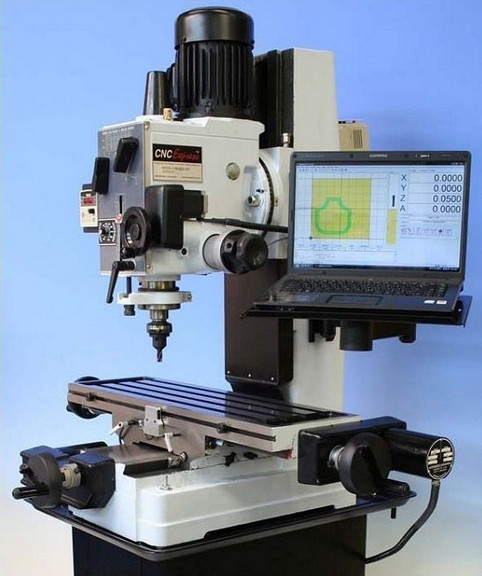
\includegraphics[width=0.5\textwidth]{./07-images/img-Ch1App/CNC-Milling-Machine.jpg}}
		\caption{App1-CNC Milling Machine}
		\label{fig:App1-CNC-Milling-Machine.jpg}
	\end{center}
\end{figure}

% ==========================================================
\subsection{App1-CNC Lathe Machine}
\begin{figure}[htbp]
	\begin{center}
		\frame{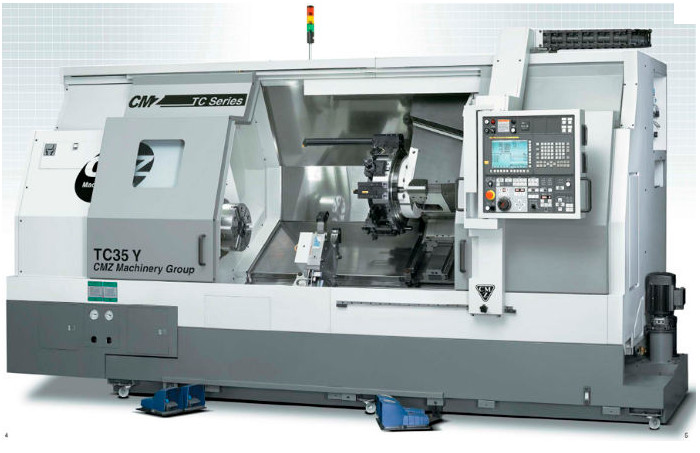
\includegraphics[width=0.5\textwidth]{./07-images/img-Ch1App/CNC-Lathe-Machine.jpg}}
		\caption{App1-CNC Lathe Machine}
		\label{fig:App1-CNC-Lathe-Machine.jpg}
	\end{center}
\end{figure}

% ==========================================================
\clearpage
\pagebreak
\subsection{App1-CNC Routing Machine}
\begin{figure}[htbp]
	\begin{center}
		\frame{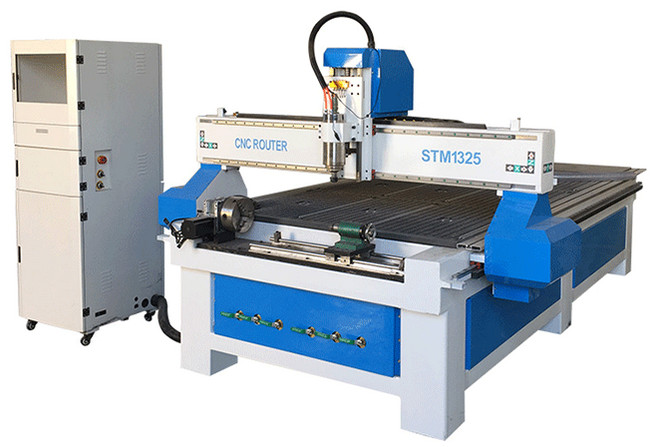
\includegraphics[width=0.50\textwidth]{./07-images/img-Ch1App/CNC-Routing-Machine.jpg}}
		\caption{App1-CNC Routing Machine}
		\label{fig:App1-CNC-Routing-Machine.jpg}
	\end{center}
\end{figure}

% ===========================================================
\subsection{App1-CNC 3D Printing Machine}
\begin{figure}[htbp]
	\begin{center}
		\frame{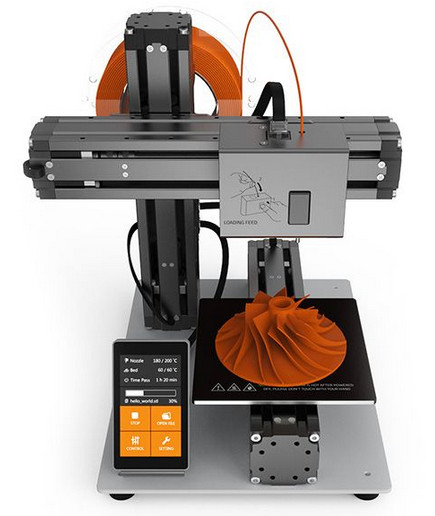
\includegraphics[width=0.5\textwidth]{./07-images/img-Ch1App/CNC-3D-Printing-Machine.jpg}}
		\caption{App1-CNC 3D Printing Machine}
		\label{fig:App1-CNC-3D-Printing-Machine.jpg}
	\end{center}
\end{figure}

% ==========================================================
 %% Introduction
	% ==========================================================
\clearpage
\pagebreak
\justifying
\renewcommand{\thesection}{B \arabic{section}}

\titleformat{\section}{\normalfont\LARGE\bfseries\color{black}}{\thesection}{10pt}{\LARGE}
\section{Appendix-B2 Literature Survey}\label{sec:App2-Literature-Survey}

% ==========================================================
\clearpage
\begin{landscape}
\subsection{App2-Ha Scilab NURBS versus Octave NURBS}
	
	\begin{table}[ht]
		\begin{center}
			\caption{App2-Scilab NURBS versus Octave NURBS}		
			\label{table:App2-Scilab NURBS versus Octave NURBS}	
			
			\begin{tabular}{ |p{0.5cm}|p{5.0cm}|p{9.0cm}|p{9.0cm}|}
				\rowcolor{gray!10}			
				\hline \multicolumn{4}{|c|}{\textbf{Scilab NURBS versus Octave NURBS}} \\ [1.0ex]
				\rowcolor{gray!10}
				\hline \textbf{No} & \textbf{Specifications}    & \textbf{Hewlett Packard EliteBook 8470p} & \textbf{Hewlett Packard ProBook 440G}\\ 
				
				\hline 1 & Name of Student    & Wan Ruslan bin W Yusoff & hello\\ 
				\hline 2 & Student ID         &  aaa & Hello\\ 
				\hline 3 & National Reg. ID   & bbb  & Hello\\ 
				\hline 4 & Faculty            & ccc  & Hello\\ 
				
				\hline
			\end{tabular}
		\end{center}
	\end{table}  
	
	
\end{landscape}
% ==========================================================
% ==========================================================
\clearpage
\begin{landscape}
	\subsection{App2-Scilab NURBS versus Octave NURBS}
	
	\begin{table}[ht]
		\begin{center}
			\caption{App2-Computer Notebook Specifications}		
			\label{tabl2:App2-Computer Notebook Specifications}	
			
			\begin{tabular}{ |p{0.5cm}|p{5.0cm}|p{9.0cm}|p{9.0cm}|}
				\rowcolor{gray!10}			
				\hline \multicolumn{4}{|c|}{\textbf{Computer Notebook Specifications}} \\ [1.0ex]
				\rowcolor{gray!10}
				\hline \textbf{No} & \textbf{Specifications}    & \textbf{Hewlett Packard EliteBook 8470p} & \textbf{Hewlett Packard ProBook 440G}\\ 
				
				\hline 1 & Name of Student    & Wan Ruslan bin W Yusoff & hello\\ 
				\hline 2 & Student ID         &  aaa & Hello\\ 
				\hline 3 & National Reg. ID   & bbb  & Hello\\ 
				\hline 4 & Faculty            & ccc  & Hello\\ 
				
				\hline
			\end{tabular}
		\end{center}
	\end{table}  
	
	
\end{landscape}
% ==========================================================
% ==========================================================

\clearpage
\begin{landscape}
	\subsection{App2-Bla bla bla}
	
	\begin{table}[ht]
		\begin{center}
			\caption{App2-Computer Notebook Specifications}		
			\label{table:App2-Computer Notebook Specifications}	
			
			\begin{tabular}{ |p{0.5cm}|p{5.0cm}|p{9.0cm}|p{9.0cm}|}
				\rowcolor{gray!10}			
				\hline \multicolumn{4}{|c|}{\textbf{Computer Notebook Specifications}} \\ [1.0ex]
				\rowcolor{gray!10}
				\hline \textbf{No} & \textbf{Specifications}    & \textbf{Hewlett Packard EliteBook 8470p} & \textbf{Hewlett Packard ProBook 440G}\\ 
				
				\hline 1 & Name of Student    & Wan Ruslan bin W Yusoff & hello\\ 
				\hline 2 & Student ID         &  aaa & Hello\\ 
				\hline 3 & National Reg. ID   & bbb  & Hello\\ 
				\hline 4 & Faculty            & ccc  & Hello\\ 
				
				\hline
			\end{tabular}
		\end{center}
	\end{table}  
	
	
\end{landscape}
% ==========================================================
% ========================================================== %% Literature Survey
	% ==========================================================
\clearpage
\pagebreak
\justifying
\renewcommand{\thesection}{C \arabic{section}}

\titleformat{\section}{\normalfont\LARGE\bfseries\color{black}}{\thesection}{10pt}{\LARGE}
\section{Appendix-C3 Research Methodology}\label{sec:App3-Research-Methodology}

% ==========================================================
\subsection{App3-Pico Universal PWM Servo Controller}\label{sec:C-3.1-Universal PWM Servo Controller Board}
				
\begin{figure}[htbp]
	\begin{center}
		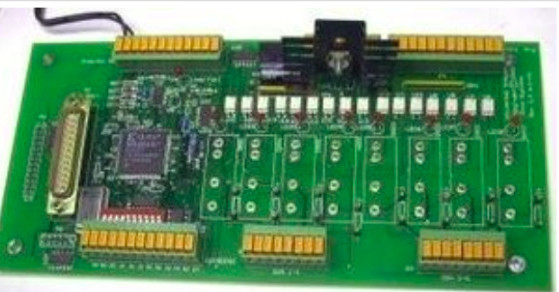
\includegraphics[width=0.85\textwidth]{./07-images/img-Ch3App/Universal-PWM-Servo-Controller.jpg}
		\caption{App3-Universal PWM Servo Controller Parallel Port Interface Board}
		\label{fig:App3-Universal-PWM-Servo-Controller.jpg}
	\end{center}
\end{figure}

\subsection{App3-Specifications Pico Universal PWM Servo Controller}

Reference: \url{http://www.pico-systems.com/motion.html}
\vspace{0.5cm}

The Universal PWM Servo Controller is a small board with everything needed to control a 2-axis, 3-axis or 4-axis machine tool with PWM-driven servo amplifiers. It contains 4 PWM generators with variable PWM drive frequency, 4 digital encoder counters to follow the machine position, 16 channels of opto-isolated digital inputs, and 8 positions for Solid State Relays of your choice to be mounted. It is connected to a computer by the parallel port. The parallel port must be at least capable of bi-directional exchange of data, but EPP or ECP modes give the best data transfer rate. The digital I/O section also implements emergency stop logic. There is an on board watchdog timer, which can be set to cause an emergency stop in case the computer fails to update the PWM generators in a timely fashion. This could shut off the servo amps, spindle motor, coolant, etc. For machines with more than 4 axes, 2 or more boards can be used together.
\vspace{0.5cm}

The computer reads the position from the encoder counters and computes a new PWM duty cycle to send to the PWM generators. This takes only about 50 uS on a 333 MHz Pentium II, so that reasonable servo update rates of 10 KHz could be made on such a machine. I usually use 1 KHz, because that is all that seems needed for machine-tool type applications.
\vspace{0.5cm}

The PWM generators divide a 10 MHz crystal clock by a minimum of 2 up to 216-1, which comes out to 5 MHz down to 153 Hz. A PWM frequency of 1 to 100 KHz is practical, and can be selected to suit the servo amplifiers. The duty cycle of the PWM waveform can be programmed in 100 nS steps, which is 1 percent at 100 KHz, but 0.2 percent at 20 KHz. The PWM and direction outputs can source or sink 12 mA to drive opto-coupled amplifier inputs.
\vspace{0.5cm}

The encoder counters keep a continuous watch over the encoder signals and can count up to 300,000 encoder counts/second, per channel. (The rev 5.x and later boards have an adjustable digital filter so that counting above 5 MHz can be performed.) They can also sense the index pulse from an encoder which has this feature. This can be used to more precisely locate the home position. If the encoder has no index channel, connect the index input (Z) to A.
\vspace{0.5cm}

The digital input section has 16 opto-isolators which can sense the condition of switches, relays, pressure switches, float sensors, etc. to allow the machine to be stopped if a fault condition occurs, sense when an axis is close to the travel limit or home position, etc. The board provides isolated 5V power to power the switches and/or sensors.
\vspace{0.5cm}

The digital output section provides sockets for up to 8 Opto-22 compatible Solid State Relays to be mounted directly onto the board. These sites are left unpopulated to allow the user to select SSRs with the output configuration and current capacity needed. A terminal strip is provided for connection to the outputs of the SSRs. LEDs monitor the command signal to each of the SSRs.
\vspace{0.5cm}

The last digital input is configured to monitor an emergency stop chain. A series circuit of normally-closed switches breaks the continuity of the circuit when an unsafe condition or problem develops (ie. spindle motor stall, servo amp overheat, lube level low, manual E-stop switch activated, etc.) An analog timer circuit can also monitor the flow of commands from the computer, and if the computer ceases updating the rate generators, then an E-stop can be caused. The E-stop condition turns off all signals to the solid state relays, as well as stopping the PWM generators, to bring the machine to a safe stop.
\vspace{0.5cm}

This boards contains a power regulator that produces all power needed by it from a provided 'wall-wart' type plug-in power supply.
\vspace{0.5cm}

The Universal PWM Controller takes advantage of the IEEE-1284 hardware signalling protocol, allowing multiple register addresses to be selected and transfers accomplished with minimum CPU overhead, and maximum data transfer rate. This requires a parallel port that can operate in the ECP or EPP mode. A male-female DB-25 cable specifically designed for IEEE-1284 compatability is required. Note: You MUST use a cable marked "IEEE-1284 compliant" for this system to work reliably.

% ==========================================================
\pagebreak
\subsection{App3-MCU Microchip 28-Pin LIN Development Board}\label{sec:C-3.3-MCU Microchip 28-Pin LIN Development Board}
				
\begin{figure}[htbp]
	\begin{center}
		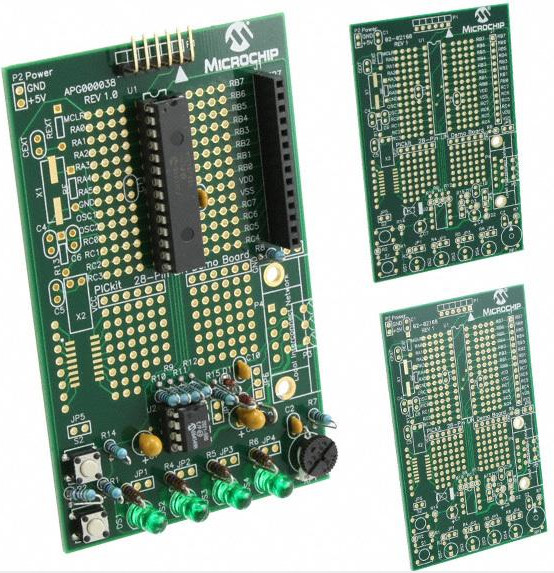
\includegraphics[width=0.95\textwidth]{./07-images/img-Ch3App/MCU-Microchip-Dev-Demo-Board.jpg}
		\caption{App3-MCU Microchip 28-Pin LIN Development Demo Interface Board}
		\label{fig:App3-MCU-Microchip-Dev-Demo-Board.jpg}
	\end{center}
\end{figure}

\subsection{App3-Specifications MCU Microchip 28-Pin LIN Development Board}

Reference: \url{https://www.digikey.my/products/en?keywords=DM164130-3-ND\%20\%20}\\
28-Pin LIN DEMO BOARD USER'S GUIDE\\
2009 Microchip Technology Inc.DSxxxxx\\
\vspace{0.5cm}

The 28-Pin LIN (Local Interconnect Network) Demo Board is a small and simple demonstration PCB for Microchip's 28-pin Dual Inline Package (DIP) PIC Microcontroller Units (MCU). It is populated with a PIC16F886 MCU, a MCP2021 LIN Transceiver with voltage regulator, four LEDs, 2 push buttons and a potentiometer. The demo board has several test points to access the I/O pins of the MCU and a generous prototyping area. The MCU can be programmed with the PICkit 2 Microcontroller Programmer or the MPLAB ICD 2 using the RJ-11 to 6-pin inline adapter (AC164110).
\vspace{0.5cm}

LIN (Local Interconnect Network) is an automotive networking technology, a sub-bus system based on a serial communications protocol. The bus is a single master/multiple slave bus that uses a single wire to transmit data.
\vspace{0.5cm}

The 28-Pin LIN Demo Board can be used with virtually any 28-pin Dual Inline Package (DIP) PIC MCU. The assembled 28-Pin LIN Demo Board is populated with a PIC16F886-I/P microcontroller. Additional 28-Pin LIN Demo Boards can be ordered from Microchip technology and distributors. Part number, DM164120-3, comes with one assembled and two blank 28-Pin LIN Demo Boards. 
\vspace{0.5cm}

The blank demo board can be used for evaluating or prototyping circuits using any of the 28-pin devices listed below.

\begin{figure}[htbp]
	\begin{center}
		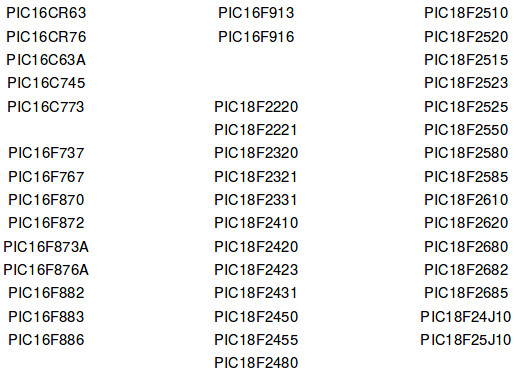
\includegraphics[width=0.85\textwidth]{./07-images/img-Ch3App/MCU-Chips-Supported-for-Dev-Demo-Board.jpg}
		\caption{App3-MCU Chips Supported-for Dev Demo Interface Board}
		\label{fig:App3-MCU-Chips-Supported-for-Dev-Demo-Board.jpg}
	\end{center}
\end{figure}

The 28-Pin LIN Demo Board is populated with a PIC16F886 MCU (U1), a MCP2021 LIN Transceiver with Voltage Regulator (U2), four LEDs (DS1-DS4), Two push buttons (SW1 and SW2), 32 KHz crystal (X2) and potentiometer (RP1). The board layout is shown in the figure below. The demo board has several test points to access the I/O pins of the MCU and a generous prototyping area. The MCU can be programmed with the PICkit 2 Microcontroller Programmer from header P1.
\vspace{0.5cm}

\pagebreak
\begin{figure}[htbp]
	\begin{center}
		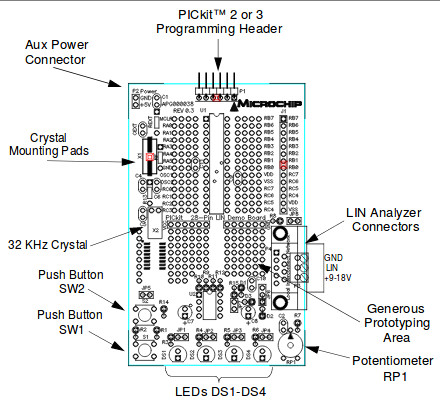
\includegraphics[width=0.95\textwidth]{./07-images/img-Ch3App/MCU-Microchip-28-Pin-LIN-Dev-Demo-Board.jpg}
		\caption{App3-MCU Microchip 28-Pin LIN Dev Demo Board Layout Diagram}
		\label{fig:App3-MCU-Microchip-28-Pin-LIN-Dev-Demo-Board.jpg}
	\end{center}
\end{figure}



% ==========================================================
\pagebreak
\subsection{App3-MCU Microchip Curiosity Development Board}\label{sec:C-3.5-Curiosity-Development-Board}

\begin{figure}[htbp]
	\begin{center}
		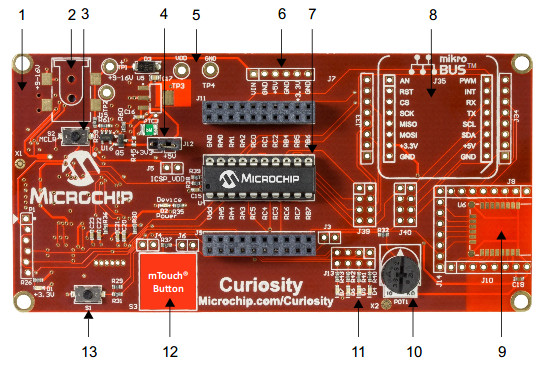
\includegraphics[width=0.85\textwidth]{./07-images/img-Ch3App/MCU-Curiosity-Dev-Board-Layout.jpg}
		\caption{App3-MCU Microchip Curiosity Demo Board Layout Diagram}
		\label{fig:App3-MCU-Curiosity-Dev-Board-Layout.jpg}
	\end{center}
\end{figure}
\begin{figure}[htbp]
	\begin{center}
		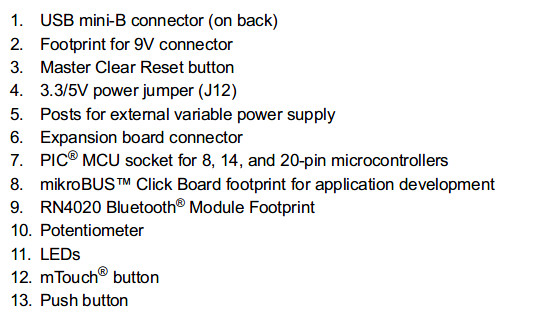
\includegraphics[width=0.65\textwidth]{./07-images/img-Ch3App/MCU-Curiosity-Dev-Board-Layout-Legend.jpg}
		\caption{App3-MCU Microchip Curiosity Demo Board Layout Legend}
		\label{fig:App3-MCU-Curiosity-Dev-Board-Layout-Legend.jpg}
	\end{center}
\end{figure}

\pagebreak
\subsection{App3-Specifications MCU Microchip Curiosity Development Board}
Reference: Curiosity Development Board User's Guide\\
2015-2016 Microchip Technology Inc. DS40001804B\\
\vspace{0.5cm}

The Curiosity Development Board supports Microchip's 8-pin, 14-pin and 20-pin 8-bit PIC MCUs. Dual-row expansion headers on either side of the socket offer flexibility of connectivity to all pins on the PIC MCUs. This board provides flexibility for 
experimentation through an application header with ground (GND) and supply voltage (VDD) connections. It also includes
a set of indication LEDs, mTouch button and push-button switches, and a variable potentiometer. Additionally, it features a 
Bluetooth low-energy footprint and a mikroBUS footprint to accommodate a variety of plug-in Click Board sensors that can be used in application development.
\vspace{0.5cm}

The Curiosity Development Board can be powered in one of three ways, depending on its usage.
\vspace{0.5cm}

\textbf{Power1 via USB Connector (J2)}\\

The USB connector (J2) will power the entire Curiosity Development Board. A shunt jumper must be placed onto jumper J12. The right two pins of J12 will connect +5V from the USB connector J2. The left two pins of J12 will connect +3.3V from the USB voltage regulator on the back side of the development board. With USB power connected to J2, power LED D1 will always be ON to indicate that +3.3V is available on the board. 
\vspace{0.5cm}

\textbf{Power2 via 9V External Power Supply (J15)}\\
%\vspace{0.5cm}

The 9V external power supply (J15) will also power the entire Curiosity Development Board. A shunt jumper must be placed onto jumper J12. The right two pins of J12 will connect +5V from the on-board voltage regulator circuitry connected to connector J15. The left two pins of J12 will connect +3.3V from the on-board voltage regulator circuitry. With 9V external power connected to J15, power LED D1 will always be ON to indicate that +3.3V is available on the board. Power LED D2 will only be ON when power (+3.3V or +5V) is applied to VDD via a shunt jumper placed on J12.
\vspace{0.5cm}

\textbf{Power3 via Variable External Power Supply (TP3, TP4)}\\
%\vspace{0.5cm}

A variable external power supply connected to TP3 and TP4 will power the entire Curiosity Development Board. A shunt jumper is not needed on J12, thus either +3.3V or +5V can be directly applied via a variable external power supply to VDD.
\vspace{0.5cm}


\textbf{Getting Started on Curiosity Board}\\
%\vspace{0.5cm}

The Curiosity Development Board must be used with MPLAB X Integrated Development Environment (IDE), available free on Microchip's web site, www.microchip.com. Use version v3.05 or later. The Curiosity Development Board, through MPLAB X, is a low-voltage in-circuit debugger, as well as a low-voltage programmer, for all supported devices. In-circuit debugging allows the user to run, examine and modify programs for the supported device embedded in the Curiosity hardware. This facilitates
the debugging of firmware and hardware concurrently. Use the Curiosity Development Board with MPLAB X IDE to run, stop and single-step through programs breakpoints can be set and the processor can be reset. When the processor stops, the contents of the register are available for examination and modification.
\vspace{0.5cm}

\textbf{Programming the Curiosity Board}\\
%\vspace{0.5cm}

After connecting the Curiosity Development Board to the computer using the on-board USB connector (J2 on the back of the board), open the MPLAB X IDE. Then create a new project or open an existing project. Click on the Project Properties icon located in the project's Dashboard window.
\vspace{0.5cm}

Alternatively, the Project Properties window can be opened by clicking on File, Project Properties, or by right-clicking on 
the project name in the Projects window and clicking Properties.
\vspace{0.5cm}

And it goes on.

% ==========================================================
 %% Research Methodology
	% ==========================================================
\clearpage
\pagebreak
\justifying
\renewcommand{\thesection}{D \arabic{section}}

\titleformat{\section}{\normalfont\LARGE\bfseries\color{black}}{\thesection}{10pt}{\LARGE}
\section{Appendix-D4 Related Research Work}\label{sec:App4-Related-Research-Work}

%% PORTRAIT
%\pagebreak
%\clearpage
% ==========================================================
\clearpage
\pagebreak
\section{Some Results on Previous Projects}

Bismillah



%% PORTRAIT
\pagebreak
\clearpage
% ==========================================================
\clearpage
\pagebreak
%% \section{Images of Devices for Previous Projects}

\subsection{App4-Parallel Port Devices}. 
				
		\begin{figure}[htbp]
			\begin{center}
				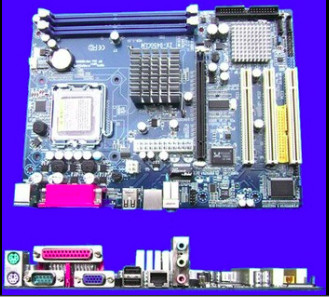
\includegraphics[width=0.700\textwidth]{./07-images/img-Ch4/Captured-Parallel-Port-Built-in-Motherboard.jpg}
				\caption{App4-Parallel Port device built-in on Motherboard (purple)}
				\label{fig:App4-Captured-Parallel-Port-Built-in-Motherboard.jpg}
			\end{center}
		 \end{figure}
		 
		
		\begin{figure}[htbp]
			\begin{center}
\frame{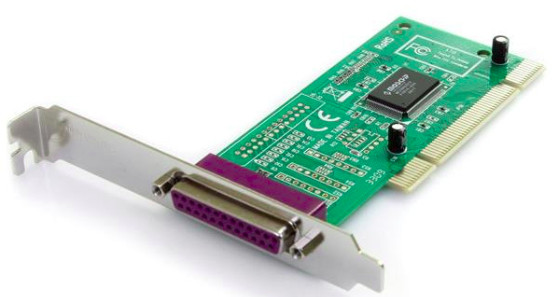
\includegraphics[width=0.65\textwidth]{./07-images/img-Ch4/Captured-Parallel-Port-PCI-Adapter-Card.jpg}}
				\caption{App4-Parallel Port PCI Adapter Card}
				\label{fig:App4-Captured-Parallel-Port-PCI-Adapter-Card.jpg}
			\end{center}
		\end{figure}
The Netmos Nm9805 is a IEEE 1284 parallel port controller with PCI bus interface. Nm9805 fully supports the existing Centronics printer interface as well as PS/2, EPP, and ECP modes. Single 5V operation. Low power. PCI compatible 1284 printer port. Multi-mode compatible controller (SPP, PS2, EPP, ECP). Fast data rates up to 1.5 Mbytes/s (parallel port). Microsoft and Linux compatible. 

% ==================
\clearpage
\pagebreak
		\begin{figure}[htbp]
			\begin{center}
\frame{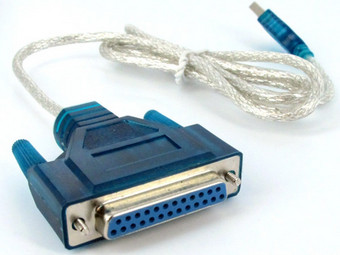
\includegraphics[width=0.65\textwidth]{./07-images/img-Ch4/Captured-USB-to-Parallel-Port-PL2305-Converter.jpg}}
				\caption{App4-USB to Parallel Port PL2305 Converter Cable}
				\label{fig:App4-Captured-USB-to-Parallel-Port-PL2305-Converter.jpg}
			\end{center}
		\end{figure}

		\begin{figure}[htbp]
			\begin{center}
\frame{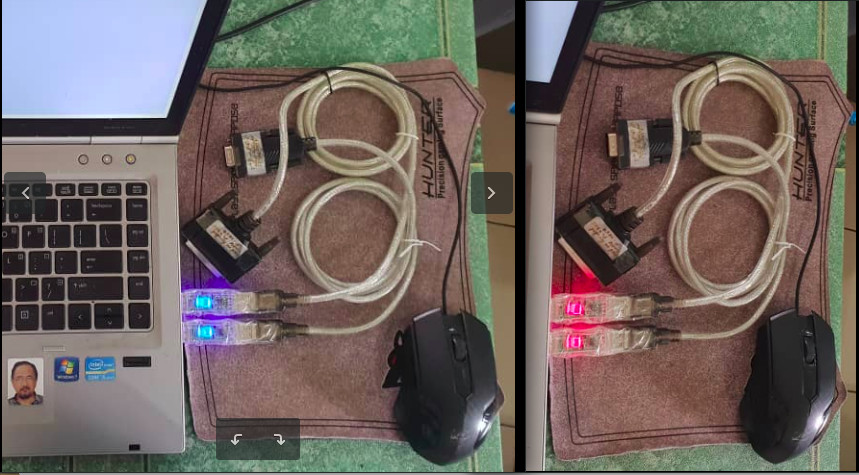
\includegraphics[width=0.75\textwidth]{./07-images/img-Ch4/USB-to-Serial-Parallel-Idle-and-Writing-Modes.jpg}}
				\caption{App4-USB to-Serial and to-Parallel Idle(Left) and Writing(Right) Modes}
				\label{fig:App4-USB-to-Serial-Parallel-Idle-and Writing-Modes.jpg}
			\end{center}
		\end{figure}
		
LEFT PICTURE: The blue color LED status is for cable device idle and ready.\\
RIGHT PICTURE: The red color LED status is for cable device busy during active reading and writing modes.  
	
\lstset{basicstyle=\ttfamily\small}
%% \lstset{basicstyle=\ttfamily\tiny}
\begin{lstlisting}[breaklines, frame=single, caption={App4-Detection of USB-to-Parallel Cable}, label=App4-usb-to-paralle-PL2305-cable-detected]
Bus 001 Device 021: ID 067b:2305 Prolific Technology, Inc. 
PL2305 Parallel Port  <=== FOUND 
[ 3978.848284] usb 1-1.6: Manufacturer: Prolific Technology Inc.
[ 3978.855271] usblp 1-1.6:1.0: usblp0: USB Bidirectional 
printer dev 21 if 0 alt 1 proto 2 vid 0x067B pid 0x2305
\end{lstlisting}

		
% ==================
\clearpage
\pagebreak
		
\subsection{App4-Velleman K8000 Parallel Interface Board}

	\begin{figure}[htbp]
		\begin{center}
\frame{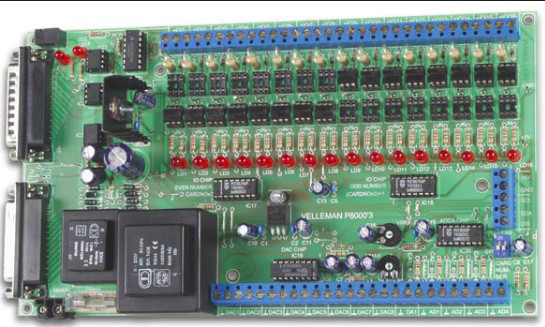
\includegraphics[width=0.85\textwidth]{./07-images/img-Ch4/Captured-Velleman-K8000-Parallel-Port-Extension-Board.jpg}}
			\caption{App4-Velleman K8000 Parallel Port Extension Board}
			\label{fig:App4-Captured-Velleman-K8000 Parallel-Port-Extension-Board.jpg}
		\end{center}
	\end{figure}
	
\lstset{basicstyle=\ttfamily\small}
%% \lstset{basicstyle=\ttfamily\tiny}
\begin{lstlisting}[breaklines, frame=single, caption={App4-Specifications of Velleman K8000 Parallel Interface Board}, label=App4-Specifications-Velleman-K8000-Interface-Board]
DIGITAL OUTPUTS:
    optocoupler, open collector output: 50mA - max. 30VDC
DIGITAL INPUTS:
    optocoupler input: 5V/5mA, max. 20V/40mA
ANALOG OUTPUTS:
    8 outputs DAC1 to DAC8, resolution: 64 steps
    minimum output voltage: 0.1V at 2mA
    maximum output voltage: 11.5V adjustable at 2mA
    resolution per step from 0.1 to 11.5V: 160mV +/- 90mV
    1 precision output DA1, resolution: 256 steps
    minimum output voltage: 0V
    maximum output voltage: 4.5V adjustable at 0.5mA
    resolution per step from 0 to 4.5V: 17.5mV
ANALOG INPUTS:
    4 analogue inputs AD1 to AD4, resolution: 256 steps
    minimum input voltage: 0V
    maximum input voltage: 5V
    input impedance: 50Mohm
    resolution: 19.5mV
    communication protocol: I2Cbus
    LED indication for each I/O
BOARD:
    25 pin D series connector for computer
    25 pin D series connector for printer
    supply voltage: 230Vac
    PCB dimensions: 237 x 133mm (9.3" x 5.2")
\end{lstlisting}			
			
%================================================		
\clearpage
\pagebreak		
		
\subsection{App4-Velleman K8055 USB Interface Board}
	
\begin{figure}[htbp]
	\begin{center}
\frame{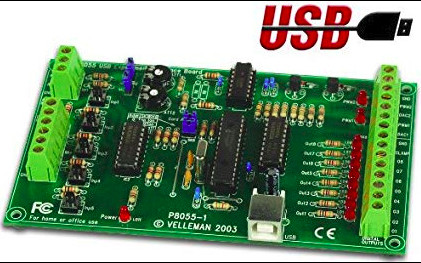
\includegraphics[width=0.85\textwidth]{./07-images/img-Ch4/Captured-Velleman-K8055-USB-Extension-Board.jpg}}
\caption{App4-Velleman K8055 USB Port Extension Board}
\label{fig:App4-Captured-Velleman-K8055-USB-Extension-Board.jpg}
	\end{center}
\end{figure}

\lstset{basicstyle=\ttfamily\small}
%% \lstset{basicstyle=\ttfamily\tiny}
\begin{lstlisting}[breaklines, frame=single, caption={App4-Specifications of Velleman K8055 USB Interface Board}, label=App4-Specifications-Velleman-K8055-USB-Interface-Board]
DIGITAL INPUTS:
    5 digital inputs (0 = ground, 1 = open) 
    (on board test buttons provided)
ANALOG INPUTS:
    2 analogue inputs with attenuation and amplification 
    option (internal test +5V provided)
DIGITAL OUTPUTS:
    8 digital open collector output switches 
    (max. 50V/100mA) (on board LED indication)
ANALOG OUTPUTS:
    2 analogue outputs:
    0 to 5V, output resistance 1K5
    PWM 0 to 100% open collector outputs 
    max 100mA / 40V (on board LED indication)
    general conversion time: 20ms per command
BOARD:    
    power supply through USB: approx. 70mA
    dimensions: 145 x 88 x 20mm / 5.7 x 3 x 0.8"
\end{lstlisting}


%================================================		
\clearpage
\pagebreak

\subsection{App4-Heber X10i USB Board}.

\begin{figure}[htbp]
	\begin{center}
		\frame{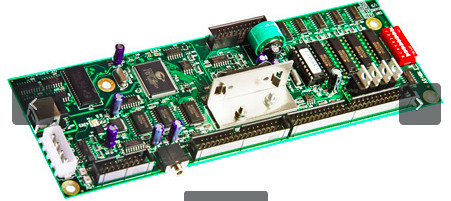
\includegraphics[width=0.85\textwidth]{./07-images/img-Ch4/Captured-Heber-X10i-USB-Extension-Board.jpg}}
		\caption{App4-Heber X10i USB Port Extension Board}
		\label{fig:App4-Captured-Heber-X10i-USB-Extension-Board.jpg}
	\end{center}
\end{figure}


\lstset{basicstyle=\ttfamily\small}
%% \lstset{basicstyle=\ttfamily\tiny}
\begin{lstlisting}[breaklines, frame=single, caption={App4-Specifications of Heber-X10i USB Interface Board}, label=App4-Specifications-Heber-X10i-USB-Interface-Board]
Heber X10i = USB real-time PC I/O controller
HARDWARE:
	64 Switched Inputs / Outputs
	Real-time I/O processor
	Battery backed SRAM
	Secure data retention
	DALLAS unique identifier
	Audio amp 5W RMS, Stereo audio amplifier
	Serial I/O
	SEC meter
	ccTalk
	LED control
	EEPROM 32KB
	Real time clock
	Current sensing 12v supply
	Open drain outputs for lamps and meters
	High current outputs
SOFTWARE:
	Serial I/O: RS232, TTL, ccTalk
	On-board security device
	Program in C, C+, C# or BlitzMax
	Microsoft Windows XPe / Linux / Raspberry Pi drivers
\end{lstlisting}

%================================================		
\clearpage
\pagebreak		
		
\subsection{App4-Arduino Due USB Board}. 

\begin{figure}[htbp]
	\begin{center}
		\frame{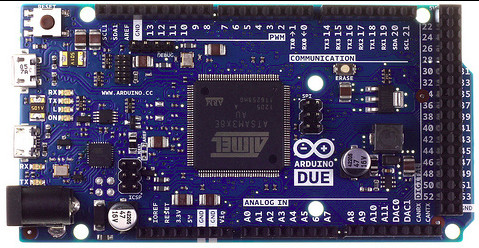
\includegraphics[width=0.85\textwidth]{./07-images/img-Ch4/Captured-Arduino-Due-USB-Extension-Board.jpg}}
		\caption{App4-Arduino Due USB Port Extension Board}
		\label{fig:App4-Captured-Arduino-Due-USB-Extension-Board.jpg}
	\end{center}
\end{figure}

Unlike most Arduino boards, the Arduino Due board runs at 3.3V. The maximum voltage that the I/O pins can tolerate is 3.3V. Applying voltages higher than 3.3V to any I/O pin could damage the board. 
\vspace*{1\baselineskip}

The SAM3X provides one hardware UART and three hardware USARTs for TTL (3.3V) serial communication.

\lstset{basicstyle=\ttfamily\small}
%% \lstset{basicstyle=\ttfamily\tiny}
\begin{lstlisting}[breaklines, frame=single, caption={App4-Specifications of Arduino Due USB Interface Board}, label=App4-Specifications-Arduino-Due-USB-Interface-Board]
Microcontroller 	AT91SAM3X8E
Operating Voltage 	3.3V
Input Voltage (recommended) 7-12V
Input Voltage (limits) 	6-16V
Digital I/O Pins 	54 (of which 12 provide PWM output)
Analog Input Pins 	12
Analog Output Pins 	2 (DAC)
Total DC Output Current on all I/O lines 	130 mA
DC Current for 3.3V Pin 	800 mA
DC Current for 5V Pin 	800 mA
Flash Memory 	512 KB all available for the user applications
SRAM 	96 KB (two banks: 64KB and 32KB)
Clock Speed 	84 MHz
Length 	101.52 mm
Width 	53.3 mm
Weight 	36 g
\end{lstlisting}

%================================================		
\clearpage
\pagebreak
		
\subsection{App4-Nexys-3 Spartan-6 FPGA USB Board}. 


\begin{figure}[htbp]
	\begin{center}
\frame{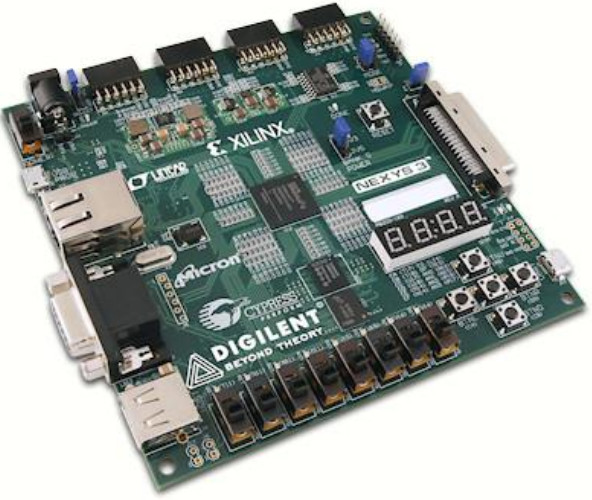
\includegraphics[width=0.80\textwidth]{./07-images/img-Ch4/Captured-Nexys3-Spartan6-FPGA-USB-Extension-Board.jpg}}
		\caption{App4-Nexys-3 Spartan-6 FPGA USB Port Extension Board}
		\label{fig:App4-Captured-Nexys3-Spartan6-FPGA-USB-Extension-Board.jpg}
	\end{center}
\end{figure}

Nexys 3 is compatible with all Xilinx CAD tools, including ChipScope, EDK, and the free WebPack. The Nexys 3 uses Digilent's newest Adept USB2 system that offers FPGA and ROM programming, automated board tests, virtual I/O, and simplified user data transfer facilities. In our project we used the Adept USB2 system.

\lstset{basicstyle=\ttfamily\small}
%% \lstset{basicstyle=\ttfamily\tiny}
\begin{lstlisting}[breaklines, frame=single, caption={App4-Specifications of Nexys-3 Spartan-6 FPGA USB Interface Board}, label=App4-Specifications-Nexys-3-Spartan-6-FPGA-USB-Interface-Board]
Xilinx Spartan-6 LX16 FPGA in a 324 pin BGA package
16 Mbyte Cellular RAM (x16)
16Mbytes SPI (quad mode) PCM non volatile memory
16Mbytes parallel PCM non volatile memory
10/100 Ethernet PHY
On board USB2 port for programming and data xfer
USB UART and USB
HID port (for mouse/keyboard)
8 bit VGA port
100 MHz CMOS oscillator
72 I/Os routed to expansion connectors
GPIO includes 8 LEDs, 5 buttons, 8 slide switches and 
4-digit seven segment display
USB v2 - programming cable included
\end{lstlisting}


%================================================		
\clearpage
\pagebreak

\subsection{App4-Raspberry Pi-3 Model-B Single Board Computer}. 

\begin{figure}[htbp]
	\begin{center}
		\frame{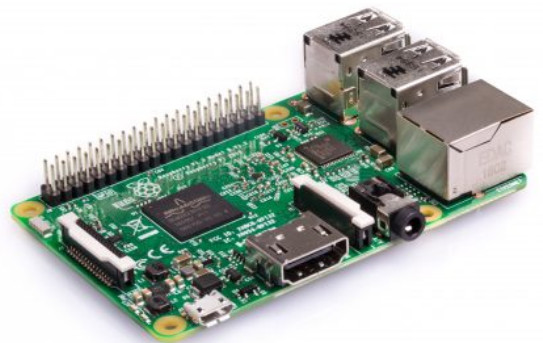
\includegraphics[width=0.85\textwidth]{./07-images/img-Ch4/Captured-Raspberry-Pi3-ModelB-SBC.jpg}}
		\caption{App4-Raspberry Pi-3 Model-B Single Board Computer}
		\label{fig:App4-Captured-Raspberry-Pi3-ModelB-SBC.jpg}
	\end{center}
\end{figure}

\subsection{App4-Raspberry Pi-2 Model-B Single Board Computer}.

\begin{figure}[htbp]
	\begin{center}
		\frame{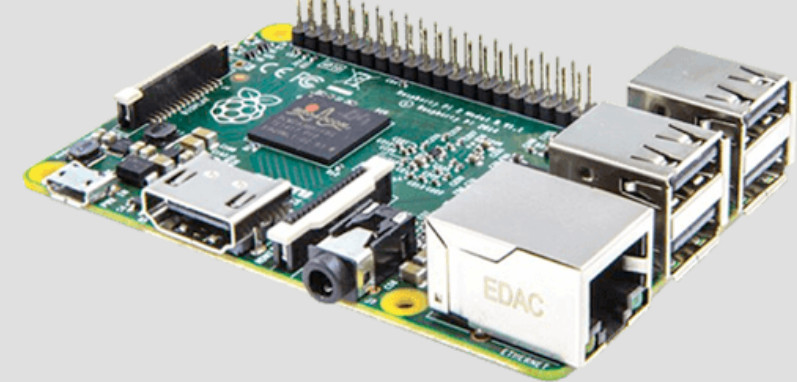
\includegraphics[width=0.85\textwidth]{./07-images/img-Ch4/Captured-Raspberry-Pi2-ModelB-SBC.jpg}}
		\caption{App4-Raspberry Pi-2 Model-B Single Board Computer}
		\label{fig:App4-Captured-Raspberry-Pi2-ModelB-SBC.jpg}
	\end{center}
\end{figure}

%================================================		
\clearpage
\pagebreak

\lstset{basicstyle=\ttfamily\small}
%% \lstset{basicstyle=\ttfamily\tiny}
\begin{lstlisting}[breaklines, frame=single, caption={App4-Specifications of Raspberry Pi 3 SBC Board}, label=App4-Specifications-of -Raspberry-Pi-3-SBC-Board]
SoC: Broadcom BCM2837
CPU: 4 x ARM Cortex-A53, 1.2GHz
GPU: Broadcom VideoCore IV
RAM: 1GB LPDDR2 (900 MHz)
Networking: 10/100 Ethernet, 2.4GHz 802.11n wireless
Bluetooth: Bluetooth 4.1 Classic, Bluetooth Low Energy
Storage: microSD
GPIO: 40-pin header, populated
Ports: HDMI, 3.5mm analogue audio-video jack, 
4 x USB 2.0, Ethernet, Camera Serial Interface (CSI), 
Display Serial Interface (DSI)
And more ....
\end{lstlisting}

\lstset{basicstyle=\ttfamily\small}
%% \lstset{basicstyle=\ttfamily\tiny}
\begin{lstlisting}[breaklines, frame=single, caption={App4-Specifications of Raspberry Pi 2 SBC Board}, label=App4-Specifications-of -Raspberry-Pi-2-SBC-Board]
SoC: Broadcom BCM2836 (CPU, GPU, DSP, SDRAM)
CPU: 900 MHz quad-core ARM Cortex A7 (ARMv7 instruction set)
GPU: Broadcom VideoCore IV @ 250 MHz
More GPU info: OpenGL ES 2.0 (24 GFLOPS); 1080p30 MPEG-2 
and VC-1 decoder (with license), h.264/MPEG-4 AVC 
high-profile decoder and encoder
Memory: 1 GB (shared with GPU)
USB ports: 4
Video input: 15-pin MIPI camera interface (CSI) connector
Video outputs: HDMI, composite video (PAL and NTSC)
via 3.5 mm jack
Audio input: I2S
Audio outputs: Analog via 3.5 mm jack; digital 
via HDMI and I2S
Storage: MicroSD
Network: 10/100Mbps Ethernet
Peripherals: 17 GPIO plus specific functions, and HAT ID bus
Power rating: 800 mA (4.0 W)
Power source: 5 V via MicroUSB or GPIO header
Size: 85.60mm x 56.5mm
Weight: 45g (1.6 oz)
\end{lstlisting}


%================================================		
\clearpage
\pagebreak

\subsection{App4-Banana Pi M2U Single Board Computer}.

\begin{figure}[htbp]
	\begin{center}
		\frame{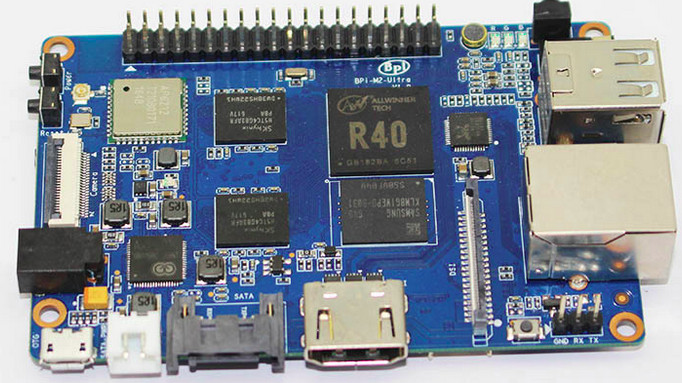
\includegraphics[width=0.85\textwidth]{./07-images/img-Ch4/Banana-PI-M2U-SBC.jpg}}
		\caption{App4-Banana Pi M2U Single Board Computer}
		\label{fig:App4-Banana-PI-M2U-SBC.jpg}
	\end{center}
\end{figure}

\lstset{basicstyle=\ttfamily\small}
%% \lstset{basicstyle=\ttfamily\tiny}
\begin{lstlisting}[breaklines, frame=single, caption={App4-Specifications of Banana Pi M2U SBC Board}, label=App4-Specifications-of -Banana-Pi-M2U-SBC-Board]
Soc 	Allwinner R40/V40
CPU 	quad-core cortex-A7,the most power efficient CPU core 
GPU 	dual-core MALI-400 MP2 and runs at 500MHz, 
GPU provides OpenGL ES 2.0, hardware-accelerated OpenVG, 
1080p45 H.264 high-profile encode and decode.
SDRAM 	2 GB DDR3 with 733MHz\(shared with GPU\)
SATA 	suppoort SATA interface
GPIO 40 Pins Header, 28 x GPIO, for UART, I2C, SPI, PWM, I2S.
On board Network 10/100/1000Mbps Ethernet\(Realtek RTL8211E)
Wifi Module 	WiFi 802.11 b/g/n \(AP 6212 module on board\)
Bluetooth 	BT4.0, Storage MicroSD\(TF\) card, 8GB eMMC 
Display 4-lane MIPI DSI display,or RGB panel, LVDS panel,
Video 	Multi-format FHD video decoding, including Mpeg1/2, 
Mpeg4, H.263, H.264, etc H.264 decode up to 1080P60,support 
Audio outputs 	HDMI, analog audio \(via 3.5 mm TRRS jack\)
Camera 	A CSI input connector Camera:Supports 8-bit YUV422 
CMOS sensor interface,Supports CCIR656 protocol for NTSC, PAL,
Supports 5M pixel camera sensor,Supports video capture 
solution up to 1080p at 30fps
Audio 	input On board microphone
USB 	2 USB 2.0 host, 1 USB 2.0 OTG
Buttons Reset button, Power button, U-boot button
Leds 	Power status Led and RJ45 Led
IR	onboard IR receiver
DC Power 5V/2A with micro USB port
battery	3.7V lithium battery power support
Sizes	85mmX56mm,same size as raspberry pi 3, Weight 40g 
\end{lstlisting}

%================================================		
\clearpage
\pagebreak

\subsection{App4-Beagle-Board xM Single Board Computer}.

\begin{figure}[htbp]
	\begin{center}
		\frame{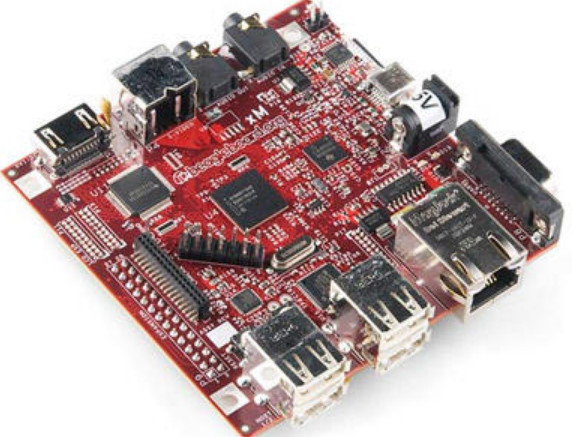
\includegraphics[width=0.85\textwidth]{./07-images/img-Ch4/Beagle-Board-xM-SBC.jpg}}
		\caption{App4-Beagle-Board xM Single Board Computer}
		\label{fig:App4-Beagle-Board-xM-SBC.jpg}
	\end{center}
\end{figure}

\lstset{basicstyle=\ttfamily\small}
%% \lstset{basicstyle=\ttfamily\tiny}
\begin{lstlisting}[breaklines, frame=single, caption={App4-Specifications of Beagle Board xM SBC Board}, label=App4-Specifications-of-Beagle-Board-xM-SBC-Board]
    Processor TI DM3730 Processor 1 GHz ARM Cortex-A8 core
    HD capable TMS320C64x+ core (800 MHz - 720p 30 fps)
    Imagination Technologies PowerVR SGX 2D/3D 
    graphics processor supporting dual independent displays
    512 MB LPDDR RAM, MicroSD/MMC card
    4 GB microSD card supplied with the BeagleBoard-xM 
    and loaded with The Angstrom Distribution
    DVI-D (HDMI connector chosen for size - maximum 
    resolution is 1400x1050)  S-Video
    USB OTG (mini AB), 4 USB ports, Ethernet
    Stereo in and out jacks
    RS-232 port  JTAG connector
    Power socket (5 V barrel connector type)
    Camera port, Expansion port
    Boot code stored on the uSD card, Boot from uSD/MMC only
    Alternative Boot source button.
    Has been demonstrated using Android,[18] 
    Angstrom Linux,[19] Fedora, Ubuntu, Gentoo,
    Arch Linux ARM and Maemo Linux distributions,
    FreeBSD, the Windows CE operating system, and RISC OS.
\end{lstlisting}

%% ===============================================

\begin{flushleft}
\begin{landscape}
%% BEGIN LANDSCAPE ENTIRELY
\pagebreak
\clearpage
%===========================================================
%%% LANDSCAPE BEGINS =======================================
%% \pagebreak
%% \clearpage
%%\begin{flushleft}
%%\begin{landscape}
	
% =========================================================
\subsection{App4-Summary main() function C-Code listing for RTAI}

% ==========================================================
\lstset{basicstyle=\footnotesize, numberstyle=\tiny\color{blue}, frame=single, numbers=left, firstnumber=1, stepnumber=1, numbersep=1pt, xleftmargin=2.0em, framexleftmargin=1.5em, xrightmargin=0.0em, breaklines=true, breakatwhitespace=false, breakindent=5pt, prebreak=\space, postbreak=\space }
% ==========================================================

\begin{lstlisting}[caption={App4-Summary main() function C-Code listing for RTAI}, label=App4-Summary main() function C-Code listing for RTAI]

// File: rtai-CNC14.c
// Date: May 05, 2018 10:04
// Author: WRY
// =========================================================
int main(int argc, char* argv[]) {
// =========================================================
WRY00_Print_DateTime_Usec(); 
printf("Bismillah from WRY executed in main().\n\n");
	
// FOR KEYBOARD INTERRUPT TO STOP (e.g. <Ctrl-C>) EXECUTION
	signal(SIGTERM, WRYcleanup);
	signal(SIGINT,  WRYcleanup);
	signal(SIGKILL, WRYcleanup);
// INVOKE FUNCTIONS SEQUENTIALLY TO RUN RTAI
	system("./load-rtai-modules.sh"); // LOAD RTAI KERNEL MODULES
	WRY01_Create_and_Initialize_Real_Time_Task_LXRT();
	WRY02_Get_Address_and_Name_of_Real_Time_Task_LXRT();
	WRY31_Make_Hard_Real_Timer_Run(); 
	WRY32_Check_Selected_Hard_Real_Time_Run_Mode(); 
	WRY33_Execute_Selected_Hard_Real_Time_Run_Mode();
	WRY04_Allow_NonRoot_Users_For_Hard_Real_Time();
	WRY05_Lock_Memory_Swapping_For_Hard_Real_Time();
	WRY06_ParallelPort_Request_StartUp_and_Enable_IRQ(); 
	WRY07_ParallelPort_Check_RT_Task_Running_Mode();
	WRY08_Start_Run_CNC_Machine();
	WRY09_Stop_Run_CNC_Machine();
	system("./unload-rtai-modules.sh"); // UNLOAD RTAI KERNEL MODULES

WRY00_Print_DateTime_Usec(); 
printf("Alhamdulillah from WRY executed in main().\n"); 
return (0);
}
\end{lstlisting}

\pagebreak
%% =========================================================
\subsection{App4-Full C-Code listing for Real Time (RTAI)}
% ==========================================================
\lstset{basicstyle=\footnotesize, numberstyle=\tiny\color{blue}, frame=single, numbers=left, firstnumber=1, stepnumber=1, numbersep=1pt, xleftmargin=2.0em, framexleftmargin=1.5em, xrightmargin=0.0em, breaklines=true, breakatwhitespace=false, breakindent=5pt, prebreak=\space, postbreak=\space }
% ==========================================================
%% \begin{lstlisting}[caption={Putting listing codes in landscape format}, label=how-to-display-in-landscape]
\begin{lstlisting}[caption={App4-Full C-Code listing for Real Time (RTAI)}, label=App4-Full C-Code listing for Real Time (RTAI)]
// File: rtai-CNC14.c
// Date: May 05, 2018 10:04
// Author: WRY
// 
// =========================================================
// (1) The prefixes WRY and TASK were used extensively in
// order to differentiate our own defined variables and functions 
// from standard C/C++ and RTAI libraries defined variables and functions.
// 
// (2) We must either link our C/C++ program against liblxrt or we 
// have to configure RTAI with "CONFIG_RTAI_LXRT_STATIC_INLINE=y".
// during linux kernel compilation.
//
// =========================================================
// STANDARD C/C++ HEADER FILES USED
// ========================================================= 

	#include <sched.h>	// Scheduler
	#include <stdio.h>	// Standard Input/Output 
	#include <stdlib.h> 	// Standard Library
	#include <time.h>	// For local date-time with usec
	#include <signal.h> 	// Signal for user interrupts, <Ctrl>-C to stop 
	#include <fcntl.h>  	// For file control
	#include <math.h>	// Mathematical functions
	#include <unistd.h> 	// Low level constants, types, function declarations
	#include <errno.h>	// Printing C errors
	#include <string.h>	// Handling strlen IN gcode . h
	#include <curses.h>	// Handling getch () , wgetch ()
	#include <sys/ioctl.h>	// System Input/Output control
	#include <sys/io.h>	// System Input/Output
	#include <sys/mman.h>	// System Memory Manager
	#include <sys/time.h>	// For system local date-time with usec




// ========================================================
// REALTIME HEADER FILES (RTAI)
// ========================================================
	#include <rtai.h>		// RTAI configuration switches (User space and Kernel space)
	#include <rtai_lxrt.h>  	// RTAI User Space libraries

// =========================================================
// RTAI VER. 5.1 DOCUMENTATION REFERENCES
// =========================================================
/*
	For full RTAI Ver 5.1 LOCAL DOCUMENTATION
		file:///usr/realtime/share/doc/rtai-5.1/html/api/files.html
	For <rtai.h>
		file:///usr/realtime/share/doc/rtai-5.1/html/api/rtai_8h_source.html
	For <rtai_lxrt.h>
		file:///usr/realtime/share/doc/rtai-5.1/html/api/rtai__lxrt_8h.html
	For <rtai_sem.h>
		file:///usr/realtime/share/doc/rtai-5.1/html/api/rtai__sem_8h.html
	For <rtai_sched.h>
		file:///usr/realtime/share/doc/rtai-5.1/html/api/rtai__sched_8h_source.html
	For <rtai_usi.h>
		file:///usr/realtime/share/doc/rtai-5.1/html/api/rtai__usi_8h_source.html
*/
// =========================================================
// EXAMPLE USAGE OF RTAI FUNCTIONS (INTERRUPT-BASED)
// ========================================================= 
/*	rt_set_oneshot_mode();
	rt_set_periodic_mode();
	start_rt_timer();
	rt_request_irq_task(PARPORT_IRQ, WRY_RT_task, RT_IRQ_TASK, 1)
	rt_task_init(); 
	rt_task_make_periodic(); 
	rt_make_hard_real_time();
	rt_make_soft_real_time();
	rt_allow_nonroot_hrt();
	rt_task_delete(WRY_RT_task);
	stop_rt_timer();
*/

// ========================================================-
// RTAI DEFINED FUNCTIONS
// =========================================================
/*
	static void * 		rt_get_adr (unsigned long name);
		Get an object address by its name. 
		Returns the address associated to name on success, 0 on failure 
	
	static unsigned long 	rt_get_name (void *adr);
		Get an object name by its address. 
		Returns the address associated to name on success, 0 on failure 
	
	static RT_TASK * 	rt_task_init (unsigned long name, int priority, int stack_size, int max_msg_size);
		Create an RTAI task extension for a Linux process/task in user space.
	
	static void 		rt_make_soft_real_time (void);
		Return a hard real time Linux process, or pthread to the standard Linux behavior.
	
	static void 		rt_make_hard_real_time (void);
		Give a Linux process, or pthread, hard real time execution capabilities allowing full kernel preemption
	
	static void 	rt_allow_nonroot_hrt (void);
		Allows a non root user to use the Linux POSIX soft real time process management and memory lock functions, and allows it to do any input-output operation from user space.
*/
// ========================================================
// GLOBAL DEFINITIONS
// ========================================================
	#define PERIOD		500000		// nanoseconds
	#define TICK_TIME	1000000		// nanoseconds
	// #define CPUMAP 	0xF  		// 16-cpus
	#define CPUMAP		0x4		// 4-cpus
	
	// BUILT_IN PARALLEL PORT ON MOTHERBOARD
	// #define PARPORT_IRQ	7
	// #define BASEPORT	0x378
	
	// HARDWARE 1 = parport0: PC-style at 0xd010 (0xd000), irq 18
	#define BASEPORT	0xd010
	#define PARPORT_IRQ	18

	// HARDWARE 2 = parport1: PC-style at 0xe100, irq 17
	// #define BASEPORT	0xe100
	// #define PARPORT_IRQ	17

	static volatile int ovr, intcnt, retval, maxcnt;

// =========================================================
// HARDWARE DEVICES PARALLEL PORT SEARCH
// =========================================================
/* EXECUTE SYSTEM FUNCTION
root@dell-ub1604-64b:/home/wruslan# dmesg | grep parp

KERNEL MESSAGE - FOUND PARALLEL PORT NO. 1
	[    8.989048] parport0: PC-style at 0xd010 (0xd000), irq 18, using FIFO [PCSPP,TRISTATE,COMPAT,EPP,ECP]
	[    9.089563] lp0: using parport0 (interrupt-driven).
	
KERNEL MESSAGE - FOUND PARALLEL PORT NO. 2
	[   11.972056] parport1: PC-style at 0xe100, irq 17 [PCSPP,TRISTATE]
	[   12.073309] lp1: using parport1 (interrupt-driven).

root@dell-ub1604-64b:/home/wruslan# lspci -v

LIST PCI DEVICE - FOUND PARALLEL PORT NO. 1
	03:00.0 Parallel controller: Oxford Semiconductor Ltd Device c110 (prog-if 02 [ECP])
	Subsystem: Oxford Semiconductor Ltd Device c110
	Flags: bus master, fast devsel, latency 0, IRQ 18
	I/O ports at d010 [size=8]
	I/O ports at d000 [size=4]
	Capabilities: [40] Power Management version 3
	Capabilities: [50] MSI: Enable- Count=1/1 Maskable- 64bit+
	Capabilities: [70] Express Legacy Endpoint, MSI 00
	Capabilities: [100] Device Serial Number 00-30-e0-11-11-00-01-10
	Capabilities: [110] Power Budgeting <?>
	Kernel driver in use: parport_pc
	Kernel modules: parport_pc

	
LIST PCI DEVICE - FOUND PARALLEL PORT NO. 2
	02:00.0 Serial controller: Device 1c00:3250 (rev 10) (prog-if 05 [16850])
	Subsystem: Device 1c00:3250
	Flags: fast devsel, IRQ 17
	I/O ports at e000 [size=256]
	Memory at f0100000 (32-bit, prefetchable) [size=32K]
	I/O ports at e100 [size=4]
	Expansion ROM at f7c00000 [disabled] [size=32K]
	Capabilities: [60] Power Management version 3
	Capabilities: [68] MSI: Enable- Count=1/32 Maskable+ 64bit+
	Capabilities: [80] Express Legacy Endpoint, MSI 00
	Capabilities: [100] Advanced Error Reporting
	Kernel driver in use: parport_serial
	Kernel modules: parport_serial

*/
// ========================================================
// REAL TIME OBJECTS
// ========================================================
	static RT_TASK* 	WRYtask;
	static RT_TASK*     	WRY_RT_task;
	struct sched_param 	WRYsched;
	struct timeval 		WRYstart, WRYfinish;
	unsigned long 		WRY_RT_task_name; 

// ========================================================
// TIMING FOR GENERAL CNC EXECUTION
// ========================================================
	static RTIME 		CNCunixtime1, CNCunixtime2;
	static RTIME		CNCstart_time_ns, CNCcurrent_time_ns;
	static RTIME		CNCend_time_ns, CNCrun_duration_ns;
	static RTIME 		CNCtimer_period_ns; // timer period, in nanoseconds
	RTIME 			CNCtimer_period_count; //actual timer period, in counts




// ========================================================
// TIMING FOR INDIVIDUAL TASK EXECUTION
// ========================================================
	struct timeval 		TASKstart, TASKfinish;
	long int		TASKusec_duration;
	double			TASKsec_duration;

// ========================================================
// GLOBAL VARIABLES (With KEYBOARD Interrupt)
// ========================================================
	int 			WRYpriority     = 0; // Highest
	int 			WRYstack_size   = 0; // Using default (512)
	int 			WRYmax_msg_size = 0; // Using default (256)
	int 			WRYpolicy 	= SCHED_FIFO;
	int 			WRYcpus_allowed	= CPUMAP;
	long int 		WRYusec_duration;
	double 			WRYsec_duration ;
	int			WRYsig;  // Keyboard interrupt signal <Ctrl>-C
	static volatile int 	ovr, intcnt, retval, maxcnt;

// =======================================================
// DEFINE REALTIME TASK STATUS AND SETTINGS
// =======================================================
// REFERNCE: Initially task status set to non-periodic (value non-zero)
// Later on in program we make task periodic (change value to 0)

	int 		WRY_RT_task_status = 1;  
	static RTIME 	WRYexpected;
	static RTIME 	WRYsampling_interval;	

// SELECT REAL TIME TIMER PERIOD
	static RTIME 	CNCtimer_period_ns = 1000*1000*1000; // means (1 sec) period

// SET REAL TIME RUN MODE (BOTH CANNOT BE TRUE)
	int 		WRY_set_periodic_mode = 1; // TRUE  = 1 
	int		WRY_set_one_shot_mode = 0; // FALSE = 0

// SELECTED RUN MODE VALUES (PERIODIC == 1, ONE-SHOT == 2)
	int 		WRY_selected_run_mode; 

// TASK PERIODIC STATUS VALUES (PERIODIC == 0, NON-PERIODIC != 0)
	int 		WRY_task_periodic_status;

// TASK ONE-SHOT STATUS VALUES (ONE-SHOT ???, NON-ONE-SHOT ???)
	int 		WRY_task_one_shot_status;




// =======================================================
// GLOBAL DATA STRUCTURES 
// =======================================================
// Used for WRY00_Print_DateTime_Usec(void) ONLY in order 
// to avoid repetitive declarations (reused) 

	time_t 		WRYtimer;
	char 		WRYbuffer[26];
	struct tm*	WRYtm_info;
	struct timeval	WRYtval_now;




// ========================================================
void WRY00_Print_DateTime_Usec(void) {
// ========================================================
// EXECUTIONS
	time(&WRYtimer);
	WRYtm_info = localtime(&WRYtimer);
	strftime(WRYbuffer, 26, "%Y-%m-%d %H:%M:%S", WRYtm_info);
	gettimeofday(&WRYtval_now, NULL);
	printf("%s", WRYbuffer);
	printf(".%09ld \t", (long int)WRYtval_now.tv_usec);
}




// =======================================================
void WRY01_Create_and_Initialize_Real_Time_Task_LXRT(void) {
// =======================================================
WRY00_Print_DateTime_Usec(); 
printf("STARTED  WRY01_Create_and_Initialize_Real_Time_Task-LXRT(void).\n");

// Create an RTAI task extension for a Linux process/task in user space.

	if (!(WRY_RT_task = rt_task_init(nam2num("CNC06"), WRYpriority, WRYstack_size, WRYmax_msg_size))) {
		WRY00_Print_DateTime_Usec();
		printf("ERROR : Cannot initialize real time task LXRT.\n");
		WRY00_Print_DateTime_Usec();
		printf("ERROR DESCRIPTION : %s\n", strerror(errno));
		exit(1);
	} else {
		WRY00_Print_DateTime_Usec();
		printf("SUCCESS: Completed real time task LXRT initialization.\n");
	}

WRY00_Print_DateTime_Usec(); 
printf("FINISHED WRY01_Create_and_Initialize_Real_Time_Task-LXRT(void).\n\n");
}

// =======================================================
void WRY02_Get_Address_and_Name_of_Real_Time_Task_LXRT(void) {
// =======================================================
WRY00_Print_DateTime_Usec(); 
printf("STARTED  WRY02_Get_Address_and_Name_of_Real_Time_Task_LXRT(void).\n");

	// GET RT_TASK NAME BY ADDRESS
	if (rt_get_name(WRY_RT_task) == 0) {
		WRY00_Print_DateTime_Usec();
		printf("ERROR : Cannot get name of real time task LXRT.\n");
		WRY00_Print_DateTime_Usec();
		printf("ERROR DESCRIPTION : %s\n", strerror(errno));
	//	exit(1);
	} else {
		WRY00_Print_DateTime_Usec();
		printf("SUCCESS: NAME of real time task LXRT = %p\n", (void *)WRY_RT_task);
		WRY_RT_task_name = (unsigned long)WRY_RT_task;
	}

WRY00_Print_DateTime_Usec(); 
printf("FINISHED WRY02_Get_Address_and_Name_of_Real_Time_Task_LXRT(void).\n\n");
}

// ========================================================
void WRY31_Make_Hard_Real_Timer_Run(void) {
// ========================================================
WRY00_Print_DateTime_Usec(); 
printf("STARTED  WRY31_Make_Hard_Real_Timer_Run(void).\n");

	// EXECUTE HARD REAL TIMER CLOCK
	rt_make_hard_real_time();
	
	// IF HARD REAL TIME ALREADY RUNNING, NOTIFY STATUS
	if (rt_is_hard_timer_running()) {
		WRY00_Print_DateTime_Usec();
		printf("SUCCESS: Hard real timer is already running.\n");
	} else {
		// IF NOT RUNNING, START WHILE LOOP
		while (!(rt_is_hard_timer_running())) {
	
			// EXECUTE HARD REAL TIMER CLOCK
			rt_make_hard_real_time();
			// IF HARD REAL TIMER IS NOT RUNNING, THEN RUN IT BY LOOPING.
			if (rt_is_hard_timer_running()) {
				WRY00_Print_DateTime_Usec();
				printf("SUCCESS: Hard real timer is NOW running.\n");
			} else {
				WRY00_Print_DateTime_Usec();
				printf("FAILED : Hard real timer is NOT YET running.\n");
				WRY00_Print_DateTime_Usec();
				printf("ERROR DESCRIPTION : %s\n", strerror(errno));
				// exit(1); // DISABLED TO KEEP ON TRYING
			} END if else    
		} // END while loop
	} // END if else

WRY00_Print_DateTime_Usec(); 
printf("FINISHED WRY31_Make_Hard_Real_Timer_Run(void).\n\n");
}

// ========================================================
void WRY32_Check_Selected_Hard_Real_Time_Run_Mode(void) {
// ========================================================
WRY00_Print_DateTime_Usec(); 
printf("STARTED  WRY32_Check_Selected_Hard_Real_Time_Run_Mode(void).\n");

	// BOTH RUN MODES SELECTED
	if ((WRY_set_periodic_mode == 1) && (WRY_set_one_shot_mode == 1)) {
		WRY00_Print_DateTime_Usec();
		printf("ERROR : Cannot select both periodic_mode and one-shot mode.\n");
		exit(1); 	
		} 
	// NO RUN MODE SELECTED
	if ((WRY_set_periodic_mode == 0) && (WRY_set_one_shot_mode == 0)) {
		WRY00_Print_DateTime_Usec();
		printf("ERROR : No hard realtime run mode selected.\n");
		exit(1); 	
		} 
	// PERIODIC MODE SELECTED
	if ((WRY_set_periodic_mode == 1) && (WRY_set_one_shot_mode == 0)) {
		WRY00_Print_DateTime_Usec();
		printf("SUCCESS: PERIODIC hard realtime run mode selected.\n");
		WRY_selected_run_mode = 1; 	
		} 
	// ONE-SHOT MODE SELECTED
	if ((WRY_set_periodic_mode == 0) && (WRY_set_one_shot_mode == 1)) {
		WRY00_Print_DateTime_Usec();
		printf("SUCCESS: ONE-SHOT hard realtime run mode selected.\n");
		WRY_selected_run_mode = 2;	
		}
WRY00_Print_DateTime_Usec(); 
printf("FINISHED WRY32_Check_Selected_Hard_Real_Time_Run_Mode(void).\n\n");
}

// ========================================================
void WRY33_Execute_Selected_Hard_Real_Time_Run_Mode(void) {
// ========================================================
WRY00_Print_DateTime_Usec(); 
printf("STARTED  WRY33_Execute_Selected_Hard_Real_Time_Run_Mode(void).\n");

	// FOR PERIODIC-MODE REAL TIME RUN
	if (WRY_selected_run_mode == 1) {
	
		WRY00_Print_DateTime_Usec();
		printf("SUCCESS: PERIODIC Set CNCtimer_period_ns \t= %lld \n", CNCtimer_period_ns);
	
		rt_set_periodic_mode();
		WRY00_Print_DateTime_Usec();
		printf("SUCCESS: PERIODIC Execute rt_set_periodic_mode().\n");

		CNCtimer_period_count=nano2count(CNCtimer_period_ns);
		WRY00_Print_DateTime_Usec();
		printf("SUCCESS: PERIODIC Execute nano2count(CNCtimer_period_ns).\n");

		WRY00_Print_DateTime_Usec();
		printf("SUCCESS: PERIODIC CNCtimer_period_count \t= %lld \n", CNCtimer_period_count);

		start_rt_timer(CNCtimer_period_count);
		WRY00_Print_DateTime_Usec();
		printf("SUCCESS: PERIODIC Execute start_rt_timer(CNCtimer_period_count).\n");

		rt_task_make_periodic(WRY_RT_task, WRYexpected, WRYsampling_interval);
		WRY00_Print_DateTime_Usec();
		printf("SUCCESS: PERIODIC Execute rt_task_make_periodic(WRY_RT_task, x, x).\n");

	} // END if PERIODIC-MODE

	// FOR ONE-SHOT MODE REAL TIME RUN
	if (WRY_selected_run_mode == 2) {
	
		rt_set_oneshot_mode();
		WRY00_Print_DateTime_Usec();
		printf("SUCCESS: ONE-SHOT Execute rt_set_oneshot_mode().\n");
		
		start_rt_timer(0);
		WRY00_Print_DateTime_Usec();
		printf("SUCCESS: ONE-SHOT Execute start_rt_timer(0).\n");
	
	} // END if ONE-SHOT MODE

WRY00_Print_DateTime_Usec(); 
printf("FINISHED WRY33_Execute_Selected_Hard_Real_Time_Run_Mode(void).\n\n");
}

// ========================================================
void WRY04_Allow_NonRoot_Users_For_Hard_Real_Time(void) {
// ========================================================
WRY00_Print_DateTime_Usec(); 
printf("STARTED  WRY04_Allow_NonRoot_Users_For_Hard_Real_Time(void).\n");

	// ALLOW NON-ROOT USERS TO HARD REAL TIME
	rt_allow_nonroot_hrt();
	WRY00_Print_DateTime_Usec();
	printf("SUCCESS: Execute Allow hard realtime for non-root users.\n");

WRY00_Print_DateTime_Usec(); 
printf("FINISHED WRY04_Allow_NonRoot_Users_For_Hard_Real_Time(void).\n\n");
}
// ========================================================
void WRY05_Lock_Memory_Swapping_For_Hard_Real_Time(void) {
// ========================================================
WRY00_Print_DateTime_Usec(); 
printf("STARTED  WRY05_Lock_Memory_Swapping_For_Hard_Real_Time(void).\n");

	// LOCK RAM MEMORY FROM MEMORY SWAPPING
	mlockall(MCL_CURRENT | MCL_FUTURE);
	WRY00_Print_DateTime_Usec();
	printf ("SUCCESS: Execute Lock memory and now no memory swapping for hard realtime.\n") ;

WRY00_Print_DateTime_Usec(); 
printf("FINISHED WRY05_Lock_Memory_Swapping_For_Hard_Real_Time(void).\n\n");
}

// ========================================================
void WRY06_ParallelPort_Request_StartUp_and_Enable_IRQ(void) {
// ========================================================
WRY00_Print_DateTime_Usec(); 
printf("STARTED  WRY06_ParallelPort_Request_StartUp_and_Enable_IRQ(void).\n");

	// The name says it, IRQs managed in user space
	// REQUEST IRQ FOR PARALLEL PORT TASK (WRY_RT_task)
		rt_request_irq_task(PARPORT_IRQ, WRY_RT_task, RT_IRQ_TASK, 1);
	
		if(!(rt_request_irq_task(PARPORT_IRQ, WRY_RT_task, RT_IRQ_TASK, 1))) {
			WRY00_Print_DateTime_Usec();
			printf("ERROR  : rt_request_irq_task(PARPORT_IRQ, WRY_RT_task, RT_IRQ_TASK, 1).\n");
			WRY00_Print_DateTime_Usec();
			printf("ERROR DESCRIPTION : %s\n", strerror(errno));
			exit(1); // Commented during testing only
		} else {
			WRY00_Print_DateTime_Usec();
			printf("SUCCESS: Display PARPORT_IRQ \t= %d\n", PARPORT_IRQ);
			
			WRY00_Print_DateTime_Usec();
			printf("SUCCESS: Display RT_IRQ_TASK \t= %d\n", RT_IRQ_TASK);
			
			WRY00_Print_DateTime_Usec();
			printf("SUCCESS: Display BASEPORT \t= 0x%02X\n", BASEPORT);
			
			WRY00_Print_DateTime_Usec();
			printf("SUCCESS: Display CPUMAP \t= 0x%02X\n", CPUMAP);
			
			WRY00_Print_DateTime_Usec();
			printf("SUCCESS: Display PERIOD \t= %d (ns)\n", PERIOD);
			
			WRY00_Print_DateTime_Usec();
			printf("SUCCESS: Display TICK_TIME \t= %d (ns)\n", TICK_TIME);
			
			WRY00_Print_DateTime_Usec();
			printf("SUCCESS: Execute rt_request_irq_task(PARPORT_IRQ, WRY_RT_task, RT_IRQ_TASK, 1).\n");
		} // END if else (rt_request)			


/* REFERENCE NOTES: ===============
		https://www.rtai.org/userfiles/documentation/magma/html/api/group__hal.html#ga74
		
		Often some of the above functions do equivalent things. Once more there is no way of doing it right except by knowing the hardware you are manipulating. Furthermore you must also remember that when you install a hard real time handler the related interrupt is usually disabled, unless you are overtaking one already owned by Linux which has been enabled by it. Recall that if have done it right, and interrupts do not show up, it is likely you have just to rt_enable_irq() your irq. 
		
	TO SOLVE PROBLEM FOR RTAI VER 5.1 = BOTH LINES BELOW ARE NOT NEEDED
		rt_startup_irq(PARPORT_IRQ);
		rt_enable_irq(PARPORT_IRQ);
============== END REFERENCE NOTES */

WRY00_Print_DateTime_Usec(); 
printf("FINISHED WRY06_ParallelPort_Request_StartUp_and_Enable_IRQ(void).\n\n");
}

// ========================================================
void  WRY07_ParallelPort_Check_RT_Task_Running_Mode(void) {
// ========================================================
WRY00_Print_DateTime_Usec(); 
printf("STARTED  WRY07_ParallelPort_Check_RT_Task_Running_Mode(void).\n");

	WRY00_Print_DateTime_Usec();
	printf("SUCCESS: Display WRY_selected_run_mode = %d\n", WRY_selected_run_mode);

	// FOR RUN PERIODIC MODE SELECTED
	if (WRY_selected_run_mode == 1) {
	
		WRY_task_periodic_status = rt_task_make_periodic(WRY_RT_task, WRYexpected, WRYsampling_interval);
	
		// IF TASK RUNNING IN PERIODIC MODE
		if (WRY_task_periodic_status == 0) {  
			WRY00_Print_DateTime_Usec();
			printf("SUCCESS: Display WRY_RT_task is ALREADY running in periodic mode.\n");
		} else {
			// LOOP WHILE NOT RUNNING IN PERIODIC MODE
			// MAKE RT_TASK RUN IN PERIODIC MODE
			while (WRY_task_periodic_status != 0) {  
	
				WRY_task_periodic_status = rt_task_make_periodic(WRY_RT_task, WRYexpected, WRYsampling_interval);
				WRY00_Print_DateTime_Usec();
				printf("SUCCESS: Execute rt_task_make_periodic(WRY_RT_task, WRYexpected, WRYsampling_interval).\n");

				if (WRY_task_periodic_status == 0) {  
					WRY00_Print_DateTime_Usec();
					printf("SUCCESS: Display WRY_RT_task is NOW running in periodic mode.\n");
				} // END if
				
			} // END while loop MAKE TASK PERIODIC
		} // END if..else TASK RUNNING
	} END if SELECTED MODE

/* REFERENCE NOTES: ================

	int rt_task_make_periodic(RT_TASK* task, RTIME start_time, RTIME period) 
		Make a task run periodically.
	
	rt_task_make_periodic mark the task task, previously created with rt_task_init(), as suitable for a periodic execution, with period period, when rt_task_wait_period() is called.
	The time of first execution is defined through start_time or start_delay. start_time is an absolute value measured in clock ticks. start_delay is relative to the current time and measured in nanoseconds.
	
	Parameters:
		task 	is a pointer to the task you want to make periodic.
		start_time 	is the absolute time to wait before the task start running, in clock ticks.
		period 	corresponds to the period of the task, in clock ticks.

	Return values:
		0 	on success. A negative value on failure as described below:
		EINVAL: task does not refer to a valid task.
================== END REFERENCE NOTES  */

WRY00_Print_DateTime_Usec(); 
printf("FINISHED WRY07_ParallelPort_Check_RT_Task_Running_Mode(void).\n\n");
}

// ========================================================
void WRY08_Start_Run_CNC_Machine(void) {
// ========================================================
WRY00_Print_DateTime_Usec(); 
printf("STARTED  WRY08_Start_Run_CNC_Machine(void).\n");

	// MAP START CNC RUNTIME IN NANO SECONDS
	CNCstart_time_ns = rt_get_time_ns();
	WRY00_Print_DateTime_Usec(); 
	printf("SUCCESS: Start CNC run at time \t= %lld (ns)\n", CNCstart_time_ns);

	// EXAMPLE EXECUTE OF CNC Signals File RUN HERE 
	int x; 
	
	// START FOR ... CONTROL LOOP THAT READS CNC SIGNALS FILE AND WRITE LINE-BY-LINE
	// THIS FOR LOOP IS A TEST FOR 10 LINES TO WRITE
	for (x = 0; x < 10; x++) {
		
		// START TIMER
		gettimeofday(&TASKstart, NULL); CNCunixtime1 = rt_get_time_ns();
		
		// EXECUTE TEST RUN IMPORTANT
		// NOTE: rt_sleep suspends execution of the caller task for  a time of delay internal count units. During this time  the CPU is used by other tasks. TIME: 1000000000 (ns) = 2893422000 (internal counts)

		// FOR COMPILATION TESTING ONLY
		// DIFFERENT HARDWARE DEVICES WILL WRITE DIFFERENTLY
		outb_p(25, BASEPORT);   // THIS IS WRITING FOR PARALLEL PORT ON LINUX

		WRY00_Print_DateTime_Usec(); 
		printf("TEST WRITING outb_p(25, BASEPORT) \n");

		// THIS SLEEP TIME IS FOR PUSLE FEEDRATE
		// rt_sleep(1000000000);
		rt_sleep(2893422000);

		WRY00_Print_DateTime_Usec(); 
		printf("run rt_sleep(2893422000) internal counts for x = %d ", x);

		// END TIMER
		CNCunixtime2 = rt_get_time_ns(); gettimeofday(&TASKfinish,NULL);
		printf("run duration = %lld (ns)\n", (CNCunixtime2 - CNCunixtime1));
		
	} // END FOR ... CONTROL LOOP (MEANS G-CODE PROCESSING ENDED)

	CNCend_time_ns = rt_get_time_ns();
	WRY00_Print_DateTime_Usec(); 
	printf("SUCCESS: End CNC run at time \t= %lld (ns)\n", CNCend_time_ns);
	
	CNCrun_duration_ns = (CNCend_time_ns - CNCstart_time_ns);
	WRY00_Print_DateTime_Usec(); 
	printf("SUCCESS: CNC total run duration\t= %lld (ns)\n", CNCrun_duration_ns);


/* REFERENCE NOTES ================= 

	CONSIDER RTAI SLEEP AND 
		rt_get_time_ns();   Nanoseconds timing in RTAI
		rt_sleep(1000000);  Equivalent to 1 second (rt_sleep is defined in micro seconds).
		rt_task_wait_period();
	
	REALTIME DRIVER FOR PARALLEL PORT OUTPUTS, MODIFIED FOR LINUX BY WRY
	REFER: Phase1D-CNC-RTOS - Report Page 161 of 204.
	
	outb_p(valout_pulse + on , BASEPORT);
	usleep(700);
	outb_p(valout_dir + on , BASEPORT);
	usleep(700);
	
	OUTB(2)              Linux Programmer's Manual                OUTB(2)	
	
	NAME
	
	outb, outw, outl, outsb, outsw, outsl, inb, inw, inl, insb, 
	insw, insl, outb_p, outw_p, outl_p, inb_p, inw_p, inl_p - port I/O

	SYNOPSIS
	#include <sys/io.h>

	unsigned char inb(unsigned short int port);
	unsigned char inb_p(unsigned short int port);
	unsigned short int inw(unsigned short int port);
	unsigned short int inw_p(unsigned short int port);
	unsigned int inl(unsigned short int port);
	unsigned int inl_p(unsigned short int port);

	void outb(unsigned char value, unsigned short int port);
	void outb_p(unsigned char value, unsigned short int port);
	void outw(unsigned short int value, unsigned short int port);
	void outw_p(unsigned short int value, unsigned short int port);
	void outl(unsigned int value, unsigned short int port);
	void outl_p(unsigned int value, unsigned short int port);

	void insb(unsigned short int port, void *addr,
	unsigned long int count);
	void insw(unsigned short int port, void *addr,
	unsigned long int count);
	void insl(unsigned short int port, void *addr,
	unsigned long int count);
	void outsb(unsigned short int port, const void *addr,
	unsigned long int count);
	void outsw(unsigned short int port, const void *addr,
	unsigned long int count);
	void outsl(unsigned short int port, const void *addr,
	unsigned long int count);

================== END REFERENCE NOTES */

WRY00_Print_DateTime_Usec(); 
printf("FINISHED WRY08_Start_Run_CNC_Machine(void).\n\n");
}

// =======================================================
void WRY09_Stop_Run_CNC_Machine(void) {
// ========================================================
WRY00_Print_DateTime_Usec(); 
printf("STARTED  WRY09_Stop_Run_CNC_Machine(void).\n");

	// RELEASE PARALLEL PORT 
	rt_release_irq_task(PARPORT_IRQ);
	WRY00_Print_DateTime_Usec(); 
	printf("SUCCESS: Execute rt_release_irq_task(PARPORT_IRQ).\n");
	
	// STOP REALTIME TIMER
	stop_rt_timer();
	WRY00_Print_DateTime_Usec(); 
	printf("SUCCESS: Execute stop_rt_timer().\n");
	
	// REVERT TO SOFT REALTIME
	rt_make_soft_real_time();
	WRY00_Print_DateTime_Usec(); 
	printf("SUCCESS: Execute rt_make_soft_real_time().\n");
	
	// DELETE REALTIME TASK
	rt_task_delete(WRY_RT_task);
	WRY00_Print_DateTime_Usec(); 
	printf("SUCCESS: Execute rt_task_delete(WRY_RT_task).\n");
	
	// NORMAL PROGRAM TERMINATION
	WRY00_Print_DateTime_Usec(); 
	printf("SUCCESS: Finished cleanup. Exiting program normally.\n");

WRY00_Print_DateTime_Usec(); 
printf("FINISHED WRY09_Stop_Run_CNC_Machine(void).\n\n");
}

// ========================================================
void WRYcleanup(int WRYsig) {
// ========================================================
printf("\n\n");
WRY00_Print_DateTime_Usec(); 
printf("STARTED  USER INTERRUPT RESPONSE TO STOP.\n");

	WRY00_Print_DateTime_Usec(); 
	printf("SUCCESS: Activate stop on User <Ctrl>-C Interrupt.\n");
	WRY00_Print_DateTime_Usec(); 
	printf("SUCCESS: Start cleanup sequence to exit program.\n");
	
	// RELEASE PARALLEL PORT 
	rt_release_irq_task(PARPORT_IRQ);
	WRY00_Print_DateTime_Usec(); 
	printf("SUCCESS: Execute rt_release_irq_task(PARPORT_IRQ).\n");
	
	// STOP REALTIME TIMER
	stop_rt_timer();
	WRY00_Print_DateTime_Usec(); 
	printf("SUCCESS: Execute stop_rt_timer().\n");
	
	// REVERT TO SOFT REALTIME
	rt_make_soft_real_time();
	WRY00_Print_DateTime_Usec(); 
	printf("SUCCESS: Execute rt_make_soft_real_time().\n");
	
	// ABNORMAL TERMINATION
	WRY00_Print_DateTime_Usec(); 
	printf("SUCCESS: Abnormal termination. Finished cleanup. Exiting program.\n");
	WRY00_Print_DateTime_Usec(); 
	printf("FINISHED USER INTERRUPT RESPONSE TO STOP.\n");
	
	// DELETE REALTIME TASK
	WRY00_Print_DateTime_Usec(); 
	printf("SUCCESS: Execute rt_task_delete(WRY_RT_task).\n\n");
	rt_task_delete(WRY_RT_task);

exit(1); // QUIT BASED ON KEYBOARD <Ctrl-C>
}




// ======================================================== 
int main(int argc, char* argv[]) {
// ========================================================
WRY00_Print_DateTime_Usec(); 
printf("Bismillah from WRY executed in main().\n\n");

// TO DO: TO INCLUDE AUTOMATIC RTAI MODULES load/unload

	// system("./load-rtai-modules.sh");
	
// FOR KEYBOARD INTERRUPT TO STOP (e.g. <Ctrl-C>)
	signal(SIGTERM, WRYcleanup);
	signal(SIGINT,  WRYcleanup);
	signal(SIGKILL, WRYcleanup);
	
// INVOKE FUNCTIONS SEQUENTIALLY TO RUN RTAI
	WRY01_Create_and_Initialize_Real_Time_Task_LXRT();
	WRY02_Get_Address_and_Name_of_Real_Time_Task_LXRT();
	WRY31_Make_Hard_Real_Timer_Run(); 
	WRY32_Check_Selected_Hard_Real_Time_Run_Mode(); 
	WRY33_Execute_Selected_Hard_Real_Time_Run_Mode();
	WRY04_Allow_NonRoot_Users_For_Hard_Real_Time();
	WRY05_Lock_Memory_Swapping_For_Hard_Real_Time();
	WRY06_ParallelPort_Request_StartUp_and_Enable_IRQ(); 
	WRY07_ParallelPort_Check_RT_Task_Running_Mode();
	WRY08_Start_Run_CNC_Machine();
	WRY09_Stop_Run_CNC_Machine();
	
	//system("./unload-rtai-modules.sh");

WRY00_Print_DateTime_Usec(); 
printf("Alhamdulillah from WRY executed in main().\n"); 
return (0);
}

// ======================================================
\end{lstlisting}

% =========================================================
% ============== BELOW IMPT TO MATCH \begin with \end ===== 
% \end{landscape}
% \end{flushleft}
% \clearpage
\pagebreak
% ==================== END OF PAGE ========================

% ==================== START OF PAGE ======================
% \pagebreak
% \clearpage
% \begin{flushleft}
%% \begin{landscape}
% =========================================================
\subsection{App4-Full execution C/C++ code for Real Time (RTAI)}
% ==========================================================
\lstset{basicstyle=\footnotesize, numberstyle=\tiny\color{blue}, frame=single, numbers=left, firstnumber=1, stepnumber=1, numbersep=1pt, xleftmargin=2.0em, framexleftmargin=1.5em, xrightmargin=0.0em, breaklines=true, breakatwhitespace=false, breakindent=5pt, prebreak=\space, postbreak=\space }
% ==========================================================
%% \begin{lstlisting}[caption={Putting listing codes in landscape format}, label=how-to-display-in-landscape]
\begin{lstlisting}[caption={App4-Full execution C/C++ code for Real Time (RTAI)}, label=App4-Full execution C/C++ code for Real Time (RTAI)]
/* COMPILATION AND EXECUTION RESULTS

(1) COMPILATION
wruslan@dell-ub1604-64b:~/ump-project2/test14$ gcc -I./ -I/usr/realtime/include -O2 -pipe -L/usr/realtime/lib -lpthread -llxrt -lm -o rtai-CNC14.x rtai-CNC14.c
wruslan@dell-ub1604-64b:~/ump-project2/test14$

(2) DISPLAY COMPILED EXECUTABLE 
wruslan@dell-ub1604-64b:~/ump-project2/test14$ ls -al
total 72
drwxrwxr-x  2 wruslan wruslan  4096 May  2 19:59 .
drwxrwxr-x 19 wruslan wruslan  4096 May  2 19:42 ..
-rwxrwxrwx  1 wruslan wruslan  4096 Apr 28 09:23 load-rtai-modules.sh
-rw-rw-r--  1 wruslan wruslan 31513 May  2 19:59 rtai-CNC14.c
-rwxrwxr-x  1 wruslan wruslan 24064 May  2 19:59 rtai-CNC14.x           <==== FOUND COMPILED EXECUTABLE
-rwxrwxrwx  1 wruslan wruslan  4063 Apr 28 09:28 unload-rtai-modules.sh
wruslan@dell-ub1604-64b:~/ump-project2/test14$

(3) EXECUTE COMPILED EXECUTABLE AS ROOT USER
wruslan@dell-ub1604-64b:~/ump-project2/test14$ sudo ./rtai-CNC14.x 
[sudo] password for wruslan: 
2018-05-02 19:59:42.000944348 	Bismillah from WRY executed in main().

2018-05-02 19:59:42.000945009 	SUCCESS: Completed real time task LXRT initialization.
2018-05-02 19:59:42.000945019 	SUCCESS: NAME of real time task LXRT = 0xffffa08f43997230
2018-05-02 19:59:42.000945038 	SUCCESS: Hard real timer is already running.
2018-05-02 19:59:42.000945045 	SUCCESS: PERIODIC hard realtime run mode selected.
2018-05-02 19:59:42.000945051 	SUCCESS: PERIODIC Set CNCtimer_period_ns 	= 1000000000 
2018-05-02 19:59:42.000945064 	SUCCESS: PERIODIC Execute rt_set_periodic_mode().
2018-05-02 19:59:42.000945076 	SUCCESS: PERIODIC Execute nano2count(CNCtimer_period_ns).
2018-05-02 19:59:42.000945083 	SUCCESS: PERIODIC CNCtimer_period_count 	= 3292519000 
2018-05-02 19:59:42.000945102 	SUCCESS: PERIODIC Execute start_rt_timer(CNCtimer_period_count).
2018-05-02 19:59:42.000945115 	SUCCESS: PERIODIC Execute rt_task_make_periodic(WRY_RT_task, x, x).
2018-05-02 19:59:42.000945128 	SUCCESS: Execute Allow hard realtime for non-root users.
2018-05-02 19:59:42.000945274 	SUCCESS: Execute Lock memory and now no memory swapping for hard realtime.
2018-05-02 19:59:42.000945281 	FINISHED WRY05_Lock_Memory_Swapping_For_Hard_Real_Time(void).

2018-05-02 19:59:42.000945288 	STARTED  WRY06_ParallelPort_Request_StartUp_and_Enable_IRQ(void).
2018-05-02 19:59:42.000945301 	SUCCESS: Display PARPORT_IRQ 	= 18
2018-05-02 19:59:42.000945308 	SUCCESS: Display RT_IRQ_TASK 	= 0
2018-05-02 19:59:42.000945315 	SUCCESS: Display BASEPORT 	= 0xD010
2018-05-02 19:59:42.000945322 	SUCCESS: Display CPUMAP 	= 0x04
2018-05-02 19:59:42.000945329 	SUCCESS: Display PERIOD 	= 500000 (ns)
2018-05-02 19:59:42.000945335 	SUCCESS: Display TICK_TIME 	= 1000000 (ns)
2018-05-02 19:59:42.000945342 	SUCCESS: Execute rt_request_irq_task(PARPORT_IRQ, WRY_RT_task, RT_IRQ_TASK, 1).
2018-05-02 19:59:42.000945348 	FINISHED WRY06_ParallelPort_Request_StartUp_and_Enable_IRQ(void).

2018-05-02 19:59:42.000945355 	STARTED  WRY07_ParallelPort_Check_RT_Task_Running_Mode(void).
2018-05-02 19:59:42.000945362 	SUCCESS: Display WRY_selected_run_mode = 1
2018-05-02 19:59:42.000945374 	SUCCESS: Display WRY_RT_task is ALREADY running in periodic mode.
2018-05-02 19:59:42.000945381 	FINISHED WRY07_ParallelPort_Check_RT_Task_Running_Mode(void).

2018-05-02 19:59:42.000945388 	STARTED  WRY08_Start_Run_CNC_Machine(void).
2018-05-02 19:59:42.000945400 	SUCCESS: Start CNC run at time 	= 1528453940458 (ns)
2018-05-02 19:59:42.000945418 	TEST WRITING outb_p(25, BASEPORT) 
2018-05-02 19:59:43.000824252 	run rt_sleep(2893422000) internal counts for x = 0 run duration = 878838671 (ns)
2018-05-02 19:59:43.000824285 	TEST WRITING outb_p(25, BASEPORT) 
2018-05-02 19:59:44.000703121 	run rt_sleep(2893422000) internal counts for x = 1 run duration = 878841400 (ns)
2018-05-02 19:59:44.000703155 	TEST WRITING outb_p(25, BASEPORT) 
2018-05-02 19:59:45.000581988 	run rt_sleep(2893422000) internal counts for x = 2 run duration = 878838807 (ns)
2018-05-02 19:59:45.000582021 	TEST WRITING outb_p(25, BASEPORT) 
2018-05-02 19:59:46.000460855 	run rt_sleep(2893422000) internal counts for x = 3 run duration = 878839578 (ns)
2018-05-02 19:59:46.000460888 	TEST WRITING outb_p(25, BASEPORT) 
2018-05-02 19:59:47.000339721 	run rt_sleep(2893422000) internal counts for x = 4 run duration = 878838160 (ns)
2018-05-02 19:59:47.000339753 	TEST WRITING outb_p(25, BASEPORT) 
2018-05-02 19:59:48.000218585 	run rt_sleep(2893422000) internal counts for x = 5 run duration = 878836793 (ns)
2018-05-02 19:59:48.000218617 	TEST WRITING outb_p(25, BASEPORT) 
2018-05-02 19:59:49.000097453 	run rt_sleep(2893422000) internal counts for x = 6 run duration = 878841787 (ns)
2018-05-02 19:59:49.000097487 	TEST WRITING outb_p(25, BASEPORT) 
2018-05-02 19:59:49.000976322 	run rt_sleep(2893422000) internal counts for x = 7 run duration = 878839913 (ns)
2018-05-02 19:59:49.000976355 	TEST WRITING outb_p(25, BASEPORT) 
2018-05-02 19:59:50.000855191 	run rt_sleep(2893422000) internal counts for x = 8 run duration = 878840543 (ns)
2018-05-02 19:59:50.000855223 	TEST WRITING outb_p(25, BASEPORT) 
2018-05-02 19:59:51.000734055 	run rt_sleep(2893422000) internal counts for x = 9 run duration = 878835850 (ns)
2018-05-02 19:59:51.000734082 	SUCCESS: End CNC run at time 	= 1537242485990 (ns)
2018-05-02 19:59:51.000734090 	SUCCESS: CNC total run duration	= 8788545532 (ns)
2018-05-02 19:59:51.000734097 	FINISHED WRY08_Start_Run_CNC_Machine(void).

2018-05-02 19:59:51.000734104 	STARTED  WRY09_Stop_Run_CNC_Machine(void).
2018-05-02 19:59:51.000734116 	SUCCESS: Execute rt_release_irq_task(PARPORT_IRQ).
2018-05-02 19:59:51.000734131 	SUCCESS: Execute stop_rt_timer().
2018-05-02 19:59:51.000734141 	SUCCESS: Execute rt_make_soft_real_time().
2018-05-02 19:59:51.000734150 	SUCCESS: Execute rt_task_delete(WRY_RT_task).
2018-05-02 19:59:51.000734156 	SUCCESS: Finished cleanup. Exiting program normally.
2018-05-02 19:59:51.000734162 	FINISHED WRY09_Stop_Run_CNC_Machine(void).

2018-05-02 19:59:51.000734171 	Alhamdulillah from WRY executed in main().
wruslan@dell-ub1604-64b:~/ump-project2/test14$ 
*/
\end{lstlisting}

% =========================================================
%\end{landscape}
%\end{flushleft}



\pagebreak
\clearpage
% ==========================================================
%%% LANDSCAPE BEGINS =======================================
% \pagebreak
% \clearpage
%\begin{flushleft}
%\begin{landscape}

% =========================================================
\subsection{App4-C++2011 Example Parallel Multithreading}
% =========================================================

\begin{enumerate}
	\item The C++ language offers for the first time support in implementing applications that require concurrent programming, regardless of the development platform. 
	
	\item Before the C++11 standard the multi-threaded applications were based on platform-specific extensions, like Intel TBB, OpenMP, Pthreads, etc. Portable applications are the major advantage brought by this new feature (i.e. Windows multi-threaded applications are easily ported to iPhone or Android platforms). 
	
	\item An advantage for those familiariazed with the Boost thread library is that many concepts from the standard C++11 library keep the same name and structure as the boost threads library classes.
	
	\item The C++ Standard Library includes classes for thread manipulation and synchronization, common protected data and low-level atomic operations. We will next exemplify and provide a general description of how these concepts occur in the C++11 Standard.
	
	\item REFERENCE: http://en.cppreference.com/w/cpp/thread
	
	\item COMPILATION \\
	Terminal\$ g++ -o multi-threaded.xx multi-threaded.cpp -std=c++11 -pthread -D\_GLIBCXX\_USE\_NANOSLEEP 
	
	\item EXECUTION\\
	Terminal\$ ./multi-threaded.xx 
	
\end{enumerate}
The 01-multi-threaded C++ program operations are described as follows: 
\begin{enumerate}
	
	\item The main C++ program spawn three threads.
	
	\item Thread-1 sleeps for 10 seconds.
	\item Thread-2 sleeps for  5 seconds.
	\item Thread-3 sleeps for  7 seconds.
	
	\item Thread-1, Thread-2 and Thread-3 are made to run some arbitrary computations to show that individual threads can do some actual useful work. For demonstration, we created three simple functions, one for each thread.  
	
	\item The sleep times were assigned to the threads to actually simulate real conditions where actual threads spent times equal to their sleep times when running actual computations. This is used to prove the time parallel nature in executions of threads.   
	
\end{enumerate}

% ==========================================================
\lstset{basicstyle=\footnotesize, numberstyle=\tiny\color{blue}, frame=single, numbers=left, firstnumber=1, stepnumber=1, numbersep=1pt, xleftmargin=2.0em, framexleftmargin=1.5em, xrightmargin=0.0em, breaklines=true, breakatwhitespace=false, breakindent=5pt, prebreak=\space, postbreak=\space }
% ==========================================================

\begin{lstlisting}[caption={App4-C++2011 Example Parallel Multithreading}, label=App4-C++2011 Example Parallel Multithreading]

// File: independent-parallel-threads-06.cpp
// Date : Sun Mar  8 12:15:41 MYT 2015 
// Author: WRY

// http://en.cppreference.com/w/cpp/thread

// COMPILATION
// THIS DOES NOT WORK
// g++  -o independent-parallel-threads-06.xx independent-parallel-threads-06.cpp -std=c++11 -pthread 

// THE FOLLOWING WORKS
// g++  -o independent-parallel-threads-06.xx independent-parallel-threads-06.cpp -std=c++11 -pthread -D_GLIBCXX_USE_NANOSLEEP 
// g++  -o independent-parallel-threads-06.xx independent-parallel-threads-06.cpp -std=gnu++11 -pthread -D_GLIBCXX_USE_NANOSLEEP 

// =========================================================

	#include <stdio.h>       // To use printf()
	#include <iostream>      // std::cout
	#include <thread>        // std::thread
	#include <ctime>	 // To use the C++ timer function
	#include <chrono>	 // To use the system_clock
	#include <mutex>	 // To run mutual exclusion (mutex) locking thread
	
	using namespace std;

// Global variables (shared among all threads for Read/Write)
	double result_wry_thread_01 = 0.0;
	double result_wry_thread_02 = 0.0;
	double result_wry_thread_03 = 0.0;
	double result_total = 0.0;

// ======================================================== 
void calculate_norm1(double x, double y, double z) {
// ========================================================
// OPENING THREAD
	std::thread::id this_id = std::this_thread::get_id();
	auto threadstart_time = std::chrono::high_resolution_clock::now();
	printf(" %lld Start wry_thread_01. Thread_ID = %x Hex. \n", threadstart_time, this_id);

// PROCESSING THREAD - DELAY (SLEEP) 10 SECONDS
	int sleep_seconds = 10;
	printf(" %lld PROCESSING wry_thread_01. Will sleep for %d seconds ... \n", threadstart_time, sleep_seconds);
	
	std::mutex g_display_mutex;
	g_display_mutex.lock();
	std::this_thread::sleep_for(std::chrono::seconds(sleep_seconds));
	g_display_mutex.unlock();
	
	result_wry_thread_01 = (x + y + z);

// CLOSING THREAD
	auto threadend_time = std::chrono::high_resolution_clock::now();
	auto duration_time = (threadend_time - threadstart_time);
	typedef std::chrono::duration<double> double_seconds;
	double process_seconds = std::chrono::duration_cast<double_seconds>(duration_time).count();
	printf(" %lld Ended wry_thread_01. Thread_ID = %x Hex. Thread processing time = %lf seconds = %lld ticks \n", threadend_time, this_id, process_seconds, duration_time);
}
// ======================================================== 
void calculate_norm2(double x, double y, double z) {
// ========================================================
// OPENING THREAD
	std::thread::id this_id = std::this_thread::get_id();
	auto threadstart_time = std::chrono::high_resolution_clock::now();
	printf(" %lld Start wry_thread_02. Thread_ID = %x Hex. \n", threadstart_time, this_id);

// PROCESSING THREAD - DELAY (SLEEP) 5 SECONDS
	int sleep_seconds = 5;
	printf(" %lld PROCESSING wry_thread_02. Will sleep for %d seconds ... \n", threadstart_time, sleep_seconds);
	
	std::mutex g_display_mutex;
	g_display_mutex.lock();
	std::this_thread::sleep_for(std::chrono::seconds(sleep_seconds));
	g_display_mutex.unlock();
	
	result_wry_thread_02 = (x/0.675 + 15.198*y + 0.005*z);    

// CLOSING THREAD
	auto threadend_time = std::chrono::high_resolution_clock::now();
	auto duration_time = (threadend_time - threadstart_time);
	typedef std::chrono::duration<double> double_seconds;
	double process_seconds = std::chrono::duration_cast<double_seconds>(duration_time).count();
	printf(" %lld Ended wry_thread_02. Thread_ID = %x Hex. Thread processing time = %lf seconds = %lld ticks \n", threadend_time, this_id, process_seconds, duration_time);
}
// ======================================================== 
void calculate_norm3(double x, double y, double z) {
// ========================================================
// OPENING THREAD
	std::thread::id this_id = std::this_thread::get_id();
	auto threadstart_time = std::chrono::high_resolution_clock::now();
	printf(" %lld Start wry_thread_03. Thread_ID = %x Hex. \n", threadstart_time, this_id);

// PROCESSING THREAD - DELAY (SLEEP) 7 SECONDS
	int sleep_seconds = 7;
	printf(" %lld PROCESSING wry_thread_03. Will sleep for %d seconds ... \n", threadstart_time, sleep_seconds);
	
	std::mutex g_display_mutex;
	g_display_mutex.lock();
	std::this_thread::sleep_for(std::chrono::seconds(sleep_seconds));
	g_display_mutex.unlock();
	
	result_wry_thread_03 = (2.56*x + y/1.56 + z*0.017); 

// CLOSING THREAD
	auto threadend_time = std::chrono::high_resolution_clock::now();
	auto duration_time = (threadend_time - threadstart_time);
	typedef std::chrono::duration<double> double_seconds;
	double process_seconds = std::chrono::duration_cast<double_seconds>(duration_time).count();
	printf(" %lld Ended wry_thread_03. Thread_ID = %x Hex. Thread processing time = %lf seconds = %lld ticks \n", threadend_time, this_id, process_seconds, duration_time);
}

// ========================================================
void print_current_date_time() {
// ========================================================
	time_t the_time;
	auto now = std::chrono::system_clock::now();
	the_time = std::chrono::system_clock::to_time_t(now);
	// std::cout << "Now : " << ctime(&tt) << std::endl;
	printf("Date Time: %s", ctime(&the_time));
}

// ========================================================
void time_ticks() {
// ========================================================
	auto ticks_wry = std::chrono::high_resolution_clock::now();
	printf(" %lld ", ticks_wry);
}

// ========================================================
int main(int argc, char *argv[]) {
// ========================================================

// OPENING MAIN PROGRAM MESSAGE
	auto start_time = std::chrono::high_resolution_clock::now();
	time_ticks(); print_current_date_time();
	time_ticks(); printf("Bismillah. Main thread started. \n");

// Threads are started by defining an object std::thread
// Spawn and launch three different threads runnung the same function
	std::thread 	wry_thread_01(calculate_norm1, 1.0, 2.0, 3.0);     
	std::thread 	wry_thread_02(calculate_norm2, 4.0, 5.0, 6.0);        
	std::thread 	wry_thread_03(calculate_norm3, 2.2, 3.2, 6.2);    

// join() - The function returns when the thread execution has completed.
// Synchronize all threads, pause until all threads finish execution.
	wry_thread_01.join();
	wry_thread_02.join();
	wry_thread_03.join();

// DISPLAY RESULTS OF INDIVIDUAL THREADS
	time_ticks(); printf("result_wry_thread_01 = %f \n", result_wry_thread_01);
	time_ticks(); printf("result_wry_thread_02 = %f \n", result_wry_thread_02);
	time_ticks(); printf("result_wry_thread_03 = %f \n", result_wry_thread_03);
	
	time_ticks(); printf("result_total = %f \n", result_wry_thread_01 + result_wry_thread_02 + result_wry_thread_03);

// CALCULATE TOTAL PROCESSING TIME
	auto end_time = std::chrono::high_resolution_clock::now();
	auto duration_time = (end_time - start_time);
	typedef std::chrono::duration<double> double_seconds;
	double process_seconds = std::chrono::duration_cast<double_seconds>(duration_time).count();
	time_ticks(); printf("TOTAL PROGRAM MULTI-THREADED PROCESSING TIME = %lf seconds = %lld ticks. \n", process_seconds, duration_time);

// CLOSING MAIN PROGRAM MESSAGE
	time_ticks(); print_current_date_time();
	time_ticks(); printf("Alhamdulillah. Main thread ended. \n");

return 0;
}
// ========================================================
\end{lstlisting}

\pagebreak
% =========================================================
\subsection{App4-C++2011 Execution Parallel Multithreading}

% ==========================================================
\lstset{basicstyle=\footnotesize, numberstyle=\tiny\color{blue}, frame=single, numbers=left, firstnumber=1, stepnumber=1, numbersep=1pt, xleftmargin=2.0em, framexleftmargin=1.5em, xrightmargin=0.0em, breaklines=true, breakatwhitespace=false, breakindent=5pt, prebreak=\space, postbreak=\space }
% ==========================================================

\begin{lstlisting}[caption={App4-C++2011 Execution Parallel Multithreading}, label=App4-C++2011 Execution Parallel Multithreading]

COMPILATION
===============
root@hpcompaqdk-ub1004-rtai:~/Documents/Multithreaded-C++11/test2.6# g++  -o independent-parallel-threads-06.xx independent-parallel-threads-06.cpp -std=c++11 -pthread -D_GLIBCXX_USE_NANOSLEEP 

EXECUTION
===============
root@hpcompaqdk-ub1004-rtai:~/Documents/Multithreaded-C++11/test2.6# ./independent-parallel-threads-06.xx 
1425871390235109 Date Time: Mon Mar  9 11:23:10 2015
1425871390235280 Bismillah. Main thread started. 
1425871390235345 Start wry_thread_02. Thread_ID = b6f28b70 Hex. 
1425871390235345 PROCESSING wry_thread_02. Will sleep for 5 seconds ... 
1425871390235340 Start wry_thread_01. Thread_ID = b7729b70 Hex. 
1425871390235340 PROCESSING wry_thread_01. Will sleep for 10 seconds ... 
1425871390235398 Start wry_thread_03. Thread_ID = b6727b70 Hex. 
1425871390235398 PROCESSING wry_thread_03. Will sleep for 7 seconds ... 
1425871395235469 Ended wry_thread_02. Thread_ID = b6f28b70 Hex. Thread processing time = 5.000124 seconds = 5000124 ticks 
1425871397235500 Ended wry_thread_03. Thread_ID = b6727b70 Hex. Thread processing time = 7.000102 seconds = 7000102 ticks 
1425871400235832 Ended wry_thread_01. Thread_ID = b7729b70 Hex. Thread processing time = 10.000492 seconds = 10000492 ticks 
1425871400235899 result_wry_thread_01 = 6.000000 
1425871400235922 result_wry_thread_02 = 81.945926 
1425871400235932 result_wry_thread_03 = 7.788682 
1425871400235939 result_total = 95.734608 
1425871400235963 TOTAL PROGRAM MULTI-THREADED PROCESSING TIME = 10.000849 seconds = 10000849 ticks. 
1425871400235969 Date Time: Mon Mar  9 11:23:20 2015
1425871400235995 Alhamdulillah. Main thread ended. 
root@hpcompaqdk-ub1004-rtai:~/Documents/Multithreaded-C++11/test2.6# 
*/
\end{lstlisting}

\pagebreak
% =========================================================
\subsection{App4-C++-MPI Example Parallel Multiprocessing}

\begin{enumerate}
	\item The 03-multi-processing.cpp C++ program is a program based on the OpenMPI library for multi-processing.
	
	\item It requires the installation of this OpenMPI libraries and executables on the particular platform.
	
	\begin{enumerate}
		
		\item COMPILATION:\\ 
		/usr/bin/mpic++ -o 03-multi-processing.xx 03-multi-processing.cpp -lpthread
		
		\item EXECUTION:\\
		/usr/bin/mpirun -np 10 03-multi-processing.xx | sort
		
		\item The number of processes to execute np above is 10. It can be changed by the user to any number preferred.
		
	\end{enumerate}
	
	\item Stage 1 : The program calculates the function kuntakinte(x), where x is an integer put as a very large number like 1000000 (one million).
	
	\item Stage 2 : The program calculates the function kamikamu(x), which is the cumulative sum of kuntakinta(x) which is the sum of kuntakinte(1) + kuntakinte(2) + kuntakinte(3) + .... + kuntakinte(x)
	
	\item The calculation of the function kuntakinta(x) itself is very CPU intensive. Study the program code for kuntakinte() function.
	
	\item The computation strategy for this OpenMPI program is "divide and conquer". Break the execution into np individual processes (multi-processing) to handle the large computation. Split the data regions for x into (x/np) individual tasks. This task is then assign to a process.
	
	\item For example, if x = 1,000,000 (one million), and np = 10, then each process will handle (1,000,000)/10 = 100,000 (one hundred thousand).
	
	\item The final result for kamikamu(1,000,000), as an example, must be the same whether we run with np=5, np=10, np=20 or any integer number because np is just the number of processes we choose to split the computation work.
	
	\item Yes. We have proven that it gave the same results for different values of np.
	
	\item The concept is similar to counting a very large pile (mountain) of oranges. The total count must be the same whether we hire 10 people, 50 people or 100 people to do the counting. The total sum cannot change. 
	
	\item This is what the current OpenMPI code 03-multi-processing.cpp does. The number of people (processes) to do the counting (computation) is np. Ha ha ha. Ya ya ya. Kah kah kah.
	
\end{enumerate}

% ==========================================================
\lstset{basicstyle=\footnotesize, numberstyle=\tiny\color{blue}, frame=single, numbers=left, firstnumber=1, stepnumber=1, numbersep=1pt, xleftmargin=2.0em, framexleftmargin=1.5em, xrightmargin=0.0em, breaklines=true, breakatwhitespace=false, breakindent=5pt, prebreak=\space, postbreak=\space }
% ==========================================================

\begin{lstlisting}[caption={App4-C++-MPI Example Parallel Multiprocessing}, label=App4-C++-MPI Example Parallel Multiprocessing]

// File: kamikamu-parallel.c
// Date: Thu Jan  3 21:53:17 MYT 2013
// Rev1: Mon Nov 18 03:45:54 MYT 2013
//
// This is a kamikamu() and kuntakinte() C-program for running parallel OpenMPI routines 
// that run on a local multicore computer or distributed on a computing cluster. 
//
// COMPILATION 
// /opt/openmpi/bin/mpicc -o kamikamu-parallel.x kamikamu-parallel.c 
// /usr/bin/mpicc -o kamikamu-parallel.x kamikamu-parallel.c 

// EXECUTION ON LOCAL MACHINE
// /opt/openmpi/bin/mpirun -np 10 kamikamu-parallel.x | sort
// /usr/bin/mpirun -np 10 kamikamu-parallel.x | sort

// EXECUTION ON CLUSTER MACHINE
// /opt/openmpi/bin/mpirun -np 10 -hostfile machines kamikamu-parallel.x | sort

// ========================================================
#include <math.h>     // For mathematical functions
#include <stdio.h>    // For function printf()
#include <stdlib.h>   // For function calloc()
#include <string.h>   // For function %s (printf string)
#include <time.h>     // For datetimestamp() function

// SET THE PATH FOR THIS HEADER FILE TO SUIT ITS LOCATION ON YOUR COMPUTER

// #include "/opt/openmpi/include/mpi.h"
#include "/usr/lib/openmpi/include/mpi.h"

// ========================================================
void datetimestamp() {
// ========================================================
	time_t ltime; 		/* calendar time */
	ltime=time(NULL); 	/* get current cal time */
	printf("%s",asctime(localtime(&ltime)));
}
// =========================================================
// DEFINE FUNCTION kuntakinte(n) THE FUNNY FUNCTION
// =========================================================
	unsigned long int kuntakinte(unsigned long int n) {
	unsigned long int m = 0;
	while (n != 1) {

		if ((n%2) == 0) {
			n = (n/2);        // FOR EVEN n
		} else { 
			n = (3*n) + 1 ;   // FOR ODD  n
		} 
		m = m + 1;

	// TRACE PRINT
	// printf("r = %d \tm = %d ", n, m);
	}

return (m);
}
// =========================================================
// DEFINE FUNCTION kamikamu(x) THE SUM ACCUMULATION FUNCTION
// =========================================================
	unsigned long int kamikamu(unsigned long int xstart, unsigned long int xend) {
	
	unsigned long int n; 
	unsigned long int kamikamu_sum = 0;

	for (n = xstart; n <= xend; n++) {
		kamikamu_sum = kamikamu_sum + kuntakinte(n);

		//TRACE PRINT
		//printf("kuntakinte(%d) = %d \t kamikamu(%d) = %d \n", n, kuntakinte(n), n, kamikamu_sum); 
	}    
	return (kamikamu_sum);
}
// ========================================================
int main(int argc, char **argv) {
// ========================================================
// VARIABLES FOR CALCULATION
	int intv_start, intv_end;
	unsigned long int interval_start, interval_end;
	unsigned long int sum, result;
	sum = 0;
	result = 0;
	
	double tStart, tEnd, tExecution;
	double tNow1, tNow2, tNow3;
	double step;
	char* cpu_name;
	int num_steps = 1000000;
	step = 1.0 / (double)num_steps;

// VARIABLES FOR OPENMPI ENVIRONMENT
	int procID, totProcesses;

// INITIALIZE OPENMPI ENVIRONMENT
	MPI_Init(&argc, &argv);
	MPI_Comm_size(MPI_COMM_WORLD, &totProcesses);
	MPI_Comm_rank(MPI_COMM_WORLD, &procID);
	cpu_name = (char *)calloc(80,sizeof(char));
	gethostname(cpu_name,80);

	if (procID == 0) {
		printf("(Q2.1B) Calculate kamikamu(1000000) using C-code with OpenMPI on local machine.\n");
		printf("PROGRAM STARTING: "); datetimestamp(); printf("\n");
	}

	// CALCULATE THE START AND END INTERVAL VALUES TO BE ASSIGNED TO EACH PROCESS
	intv_start = procID * (num_steps/totProcesses) +1;
	intv_end   = intv_start + (num_steps/totProcesses) -1;
	
	// THIS IS FOR THE LAST INTERVAL ONLY
	if (procID == (totProcesses-1)) {
		intv_end = num_steps;
	}

	interval_start = (unsigned long int)intv_start;
	interval_end   = (unsigned long int)intv_end;

	// DISPLAY START TIME FROM ALL PROCESSES
	tStart = MPI_Wtime();
	printf("%.16lf \tProcess-%d on %s. STARTED. Assigned range = (%d,%d) \n", MPI_Wtime()-tStart, procID, cpu_name, interval_start, interval_end);

	// EACH PROCESS WILL RUN THE AREA COMPUTATION FOR ITS OWN ASSIGNED INTERVAL (START AND END VALUES)
	tNow2 = MPI_Wtime();
	sum = kamikamu(interval_start, interval_end);
	tNow3 = MPI_Wtime();

	// DISPLAY COMPUTING TIME EXECUTED FOR EACH PROCESS
	printf("%.16lf \tProcess-%d on %s. Execution time = %.16lf \n", MPI_Wtime()-tStart, procID, cpu_name, (tNow3-tNow2));

	// DISPLAY COLLECTED PARTIAL SUM FROM EACH PROCESS
	printf("%.16lf \tProcess-%d on %s. PARTIAL SUM = %ld \n", MPI_Wtime()-tStart, procID, cpu_name, sum);

	// ACCUMULATE SUM FROM EACH PROCESS
	MPI_Reduce(&sum, &result, 1, MPI_INTEGER, MPI_SUM, 0, MPI_COMM_WORLD);

	// DISPLAY ONLY ON HEADNODE (OTHERWISE WILL RUN ON ALL NODES)
	if (procID == 0) {
		printf("%.16lf \tProcess-%d on %s. Effective Execution Time: %.16lf \n",  MPI_Wtime()-tStart, procID, cpu_name, MPI_Wtime()-tStart);
		printf("%.16lf \tProcess-%d on %s. kamikamu(1000000) = %ld \n", MPI_Wtime()-tStart, procID, cpu_name, result);
		printf("\n"); printf("PROGRAM FINISHED: "); datetimestamp();
	}
	MPI_Finalize();
return (0);
}
// ========================================================
\end{lstlisting}

\pagebreak
% =========================================================
\subsection{App4-C++-MPI Execution Parallel Multiprocessing}

% ==========================================================
\lstset{basicstyle=\footnotesize, numberstyle=\tiny\color{blue}, frame=single, numbers=left, firstnumber=1, stepnumber=1, numbersep=1pt, xleftmargin=2.0em, framexleftmargin=1.5em, xrightmargin=0.0em, breaklines=true, breakatwhitespace=false, breakindent=5pt, prebreak=\space, postbreak=\space }
% ==========================================================

\begin{lstlisting}[caption={App4-C++-MPI Execution Parallel Multiprocessing}, label=App4-C++-MPI Execution Parallel Multiprocessing]

COMPILE THE SPMD kamikamu-parallel.c C-PROGRAM
[clab50@clusterlab tutorial04]$ /opt/openmpi/bin/mpicc -o kamikamu-parallel.x kamikamu-parallel.c 

EXECUTE THE SPMD kamikamu-parallel.x EXECUTABLE (MUST HAVE -np 10) WITH sort OUTPUT 
[clab50@clusterlab tutorial04]$ /opt/openmpi/bin/mpirun -np 10 -hostfile machines ./kamikamu-parallel.x | sort

0.0000008846400306 	Process-7 on compute-3-2.local. STARTED. Assigned range = (700001,800000) 
0.0000009156065062 	Process-3 on compute-3-3.local. STARTED. Assigned range = (300001,400000) 
0.0000009223585948 	Process-8 on compute-3-3.local. STARTED. Assigned range = (800001,900000) 
0.0000009536743164 	Process-0 on compute-3-0.local. STARTED. Assigned range = (1,100000) 
0.0000009541399777 	Process-1 on compute-3-1.local. STARTED. Assigned range = (100001,200000) 
0.0000018946593627 	Process-9 on compute-3-4.local. STARTED. Assigned range = (900001,1000000) 
0.0000019473955035 	Process-6 on compute-3-1.local. STARTED. Assigned range = (600001,700000) 
0.0000019873259589 	Process-4 on compute-3-4.local. STARTED. Assigned range = (400001,500000) 
0.0000020727748051 	Process-5 on compute-3-0.local. STARTED. Assigned range = (500001,600000) 
0.0000021163141355 	Process-2 on compute-3-2.local. STARTED. Assigned range = (200001,300000) 
0.0973579536657780 	Process-0 on compute-3-0.local. Execution time = 0.0973269939422607 
0.0973799537168816 	Process-0 on compute-3-0.local. PARTIAL SUM = 10753840 
0.1112939541926607 	Process-1 on compute-3-1.local. Execution time = 0.1111660003662109 
0.1113159541273490 	Process-1 on compute-3-1.local. PARTIAL SUM = 12184824 
0.1144861163338646 	Process-2 on compute-3-2.local. Execution time = 0.1144130229949951 
0.1145081162685528 	Process-2 on compute-3-2.local. PARTIAL SUM = 12731265 
0.1205389156239107 	Process-3 on compute-3-3.local. Execution time = 0.1204419136047363 
0.1205629155738279 	Process-3 on compute-3-3.local. PARTIAL SUM = 13092861 
0.1223229473689571 	Process-6 on compute-3-1.local. Execution time = 0.1222000122070312 
0.1223449473036453 	Process-6 on compute-3-1.local. PARTIAL SUM = 13721423 
0.1263560727238655 	Process-5 on compute-3-0.local. Execution time = 0.1262848377227783 
0.1263840727042407 	Process-5 on compute-3-0.local. PARTIAL SUM = 13534059 
0.1266208846354857 	Process-7 on compute-3-2.local. Execution time = 0.1265420913696289 
0.1266438846942037 	Process-7 on compute-3-2.local. PARTIAL SUM = 13884901 
0.1267469873419032 	Process-4 on compute-3-4.local. Execution time = 0.1266419887542725 
0.1267699872842059 	Process-4 on compute-3-4.local. PARTIAL SUM = 13372761 
0.1284559223568067 	Process-8 on compute-3-3.local. Execution time = 0.1283540725708008 
0.1284809224307537 	Process-8 on compute-3-3.local. PARTIAL SUM = 14000042 
0.1290498946327716 	Process-9 on compute-3-4.local. Execution time = 0.1289429664611816 
0.1290728946914896 	Process-9 on compute-3-4.local. PARTIAL SUM = 14159263 
0.1308339537354186 	Process-0 on compute-3-0.local. Effective Execution Time: 0.1308329537278041 
0.1308569536777213 	Process-0 on compute-3-0.local. kamikamu(1000000) = 131435239 
PROGRAM FINISHED: Mon Nov 18 05:32:27 2013
PROGRAM STARTING: Mon Nov 18 05:32:27 2013
(Q2.1B) Calculate kamikamu(1000000) using C-code with OpenMPI on local machine.
[clab50@clusterlab tutorial04]$ 
*/
// ========================================================
\end{lstlisting}

% =========================================================
% \end{landscape}
% \end{flushleft}


\pagebreak
\clearpage
%===========================================================
%%% LANDSCAPE BEGINS =======================================
%\pagebreak
%\clearpage
%\begin{flushleft}
%\begin{landscape}

% =========================================================
\subsection{App4-Rust Parallel Multithreading Codes}
% =========================================================
\begin{enumerate}
	\item We provided the Rust program source code: rust-multi-threaded.rs
	
	\item The file suffix (.rs) is for Rust program code. We compile this Rust code using the Rust compiler (rustc)
	
	\item Rust Compiler:\\
	
	wruslan\@HP-ELBook8470p-ub1604-64b: \$ which rustc\\
		/home/wruslan/.cargo/bin/rustc\\
	
	wruslan\@HP-ELBook8470p-ub1604-64b: \$ rustc -version\\
		rustc 1.28.0 (9634041f0 2018-07-30)\\
	
	\item The resulting compiled Rust code does not have a suffix, just rust-multi-threaded.
	
	\item Child threads: In this multi-threaded Rust program, the main thread spawned three(3) child threads: thread01(x), thread02(y) and thread03(z), where x, y and z, are random integers between 1 and 20 (seconds), to simulate the sleep times of each individual child thread.
	
	\item Main thread: The main thread is made to run beyond the longest time for any one of the three(3) child threads to finish. Since each child thread will have a maximum assigned finished time of 20 seconds (sleep), we made the main thread sleep for 21 seconds. This is to ensure that all child threads will finish early and join the main thread.
	
	\item If we reduce the main thread sleep to less than 20 seconds, then some child threads would not have finished by this time. This means when the main thread dies, all the child threads get pulled and die together (whether finished or not yet finished). This is multi-threading.
	
	\item Note that the total execution time is the time the main thread runs active, which is set at 21 seconds. You can reduce this setting, to prove that it is multi-threading (as explained above).
	
	\item Proof : This total time is not the sum of the sleep times of the child threads. If it is the sum, then we have sequential-in-time execution not parallel-in-time execution. This is the proof that all child threads run independently and parallel-in-time.
	
	\item Note that the codes for Rust is much more compact than C/C++ codes. Rust was designed from the ground up with Safety, Security and Concurrency (SSC) built-into the Rust engine, not many separate software libraries, unlike C/C++ language. 
	
\end{enumerate}

\pagebreak

% ==========================================================
\lstset{basicstyle=\footnotesize, numberstyle=\tiny\color{blue}, frame=single, numbers=left, firstnumber=1, stepnumber=1, numbersep=1pt, xleftmargin=2.0em, framexleftmargin=1.5em, xrightmargin=0.0em, breaklines=true, breakatwhitespace=false, breakindent=5pt, prebreak=\space, postbreak=\space }
% ==========================================================

\begin{lstlisting}[caption={App4-Rust Parallel Multithreading Codes}, label=App4-Rust Parallel Multithreading Codes]
// File: rust-multi-threaded.rs
// Date: Sat Aug 25 15:42:16 +08 2018
// Author: WRY
// =======================================================

	use std::thread;
	use std::time::{Duration, SystemTime, UNIX_EPOCH};

// ========================================================
// SEE SOLUTION (1) BY WRY HOW TO SOLVE THIS PROBLEM
// https://crates.io/crates/rand
// About generating random numbers in Rust

	extern crate rand;
	use rand::prelude::*;
	
// ========================================================
// SEE SOLUTION (2) BY WRY HOW TO SOLVE THIS PROBLEM
// https://crates.io/crates/chrono
// About getting current date and time in Rust

	extern crate chrono;
	use chrono::prelude::*;

// ======================
// HIGH RESOLUTION TIME
// ======================

fn hires_time() {
	let start = SystemTime::now();
	let since_the_epoch = start.duration_since(UNIX_EPOCH).expect("Time went backwards");
	print!("{:?} ", since_the_epoch);
}

// SIMPLE THREAD 1
// ===========================
fn my_thread01(x: u64) {
// ===========================
	hires_time(); print!("\tStarting child thread01({:?}).\n", x);
	thread::sleep(Duration::from_millis(1000*x)); 
	hires_time(); print!("\tFinished child thread01({:?}).\n", x);	
}

// SIMPLE THREAD 2
// ===========================
fn my_thread02(y: u64) {
// ===========================
	hires_time(); print!("\tStarting child thread02({:?}).\n", y);
	thread::sleep(Duration::from_millis(1000*y)); 
	hires_time(); print!("\tFinished child thread02({:?}).\n", y);	
}

// SIMPLE THREAD 3
// ===========================
fn my_thread03(z: u64) {
// ===========================
	hires_time(); print!("\tStarting child thread03({:?}).\n", z);
	thread::sleep(Duration::from_millis(1000*z)); 
	hires_time(); print!("\tFinished child thread03({:?}).\n", z);	
}

// ========================================================
fn main() {
// ========================================================

//  TESTED GOOD RANDOM NUMBERS BASED ON SOLUTION(1) ABOVE
// 
	//  let x: u8 = random();
	//  println!("random u8 = {}", x);
	
	//  let y = random::<f64>();
	//  println!("random::<f64> = {}", y);
	
	//  let sleep_time: u8 = thread_rng().gen_range(1, 21);
	//  println!("sleep_time u8 value = {:?}", sleep_time); 

// TESTED GOOD DATE RUN TODAY NOW BASED ON SOLUTION(2) ABOVE
	// let utc: DateTime<Utc> = Utc::now();       
	// println!("DateTime<Utc> value = {}", utc);
	
	// let local: DateTime<Local> = Local::now(); 
	// println!("DateTime<Local> value = {:?}", local);

// ========================================================
// IMPLEMENTATION

	let local: DateTime<Local> = Local::now();
	hires_time(); print!("\tBismillah from WRY. DateTime now = {:?} \n", local);
	
	let sleep_time01: u64 = thread_rng().gen_range(1, 21);
	
	println!("Assigned sleep_time01 u64 value = {:?}", sleep_time01);
	thread::spawn(move || {
		hires_time();
		print!("\tMain thread spawning child thread01({:?})\n", sleep_time01);
		my_thread01(sleep_time01);
	});
	
	let sleep_time02: u64 = thread_rng().gen_range(1, 21);
	println!("Assigned sleep_time02 u64 value = {:?}", sleep_time02);

	thread::spawn(move || {
		hires_time(); 
		print!("\tMain thread spawning child thread02({:?})\n", sleep_time02);
		my_thread02(sleep_time02);
	});

	let sleep_time03: u64 = thread_rng().gen_range(1, 21);
	println!("Assigned sleep_time03 u64 value = {:?}", sleep_time03);

	thread::spawn(move || {
		hires_time(); 
		print!("\tMain thread spawning child thread03({:?})\n", sleep_time03);
		my_thread03(sleep_time03);
	});

// IMPT: Main to sleep longer than all child threads, otherwise the remaining
// child threads die together when main thread dies.
// Try reducing this sleep time and see. Ha ha ha.

	hires_time();
	print!("\tMain thread starting to sleep for max XXX seconds.\n");

	thread::sleep(Duration::from_millis(21000)); // Wait for 21 seconds.
	hires_time();print!("\tMain thread finished sleep time max for 21 seconds.\n");

	hires_time(); print!("\tAlhamdulillah from WRY.\n");
	
} // END main()

// ========================================================
/* COMPILATION 

wruslan@HP-ELBook8470p-ub1604-64b:~/Downloads/temp3$ rustc rust-multi-threaded.rs 

EXECUTION NO. 1
====================
wruslan@HP-ELBook8470p-ub1604-64b:~/Downloads/temp3$ ./rust-multi-threaded 
1535187474.12119863s 	Bismillah from WRY. DateTime now = 2018-08-25T16:57:54.121130393+08:00 
1535187474.123016112s 	Main thread spawning child thread01(4)
1535187474.12304328s 	Starting child thread01(4).
1535187474.123467714s 	Main thread starting to sleep for max 21 seconds.
1535187474.123703762s 	Main thread spawning child thread02(2)
1535187474.123724902s 	Starting child thread02(2).
1535187474.123972992s 	Main thread spawning child thread03(18)
1535187474.123986326s 	Starting child thread03(18).
1535187476.123839552s 	Finished child thread02(2).
1535187478.123198653s 	Finished child thread01(4).
1535187492.124127672s 	Finished child thread03(18).
1535187495.123586666s 	Main thread finished sleep time max for 21 seconds.
1535187495.123627182s 	Alhamdulillah from WRY.
wruslan@HP-ELBook8470p-ub1604-64b:~/Downloads/temp3$ 

ANALYSIS
1535187492.124127672s 	Finished child thread03(18).
-1535187474.123986326s 	Starting child thread03(18).
=======================
18.001  seconds HA HA HA Time for longest thread to finish.

EXECUTION No. 2
======================
wruslan@HP-ELBook8470p-ub1604-64b:~/Downloads/temp3$ ./rust-multi-threaded 
1535187502.325989233s 	Bismillah from WRY. DateTime now = 2018-08-25T16:58:22.325920986+08:00 
1535187502.32760476s 	Main thread starting to sleep for max 21 seconds.
1535187502.32786682s 	Main thread spawning child thread01(20)
1535187502.327892862s 	Starting child thread01(20).
1535187502.328241946s 	Main thread spawning child thread02(10)
1535187502.328266967s 	Starting child thread02(10).
1535187502.328634609s 	Main thread spawning child thread03(17)
1535187502.328649296s 	Starting child thread03(17).
1535187512.328427258s 	Finished child thread02(10).
1535187519.328750721s 	Finished child thread03(17).
1535187522.328023394s 	Finished child thread01(20).
1535187523.327788422s 	Main thread finished sleep time max for 21 seconds.
1535187523.32783525s 	Alhamdulillah from WRY.
wruslan@HP-ELBook8470p-ub1604-64b:~/Downloads/temp3$ 

ANALYSIS
1535187522.328023394s 	Finished child thread01(20).
-1535187502.327892862s 	Starting child thread01(20).
=======================
20.001  seconds HA HA HA Time for longest thread to finish. 

ALHAMDULILLAH 3 TIMES.
*/
// ========================================================
\end{lstlisting}

% =========================================================
%\clearpage
%\end{landscape}
%\end{flushleft}


\pagebreak
\clearpage
% ==========================================================
%%% LANDSCAPE BEGINS =======================================
\pagebreak
\clearpage
%\begin{flushleft}
%\begin{landscape}

% =========================================================
\subsection{App4-Julia Parallel Programming Codes}
% =========================================================

\begin{enumerate}

	\item \textbf{Parallel computing in Julia}
	
	\item \url{https://github.com/JuliaLang/julia/blob/master/doc/src/manual/parallel-computing.md}
	
	\item For newcomers to multi-threading and parallel computing it can be useful to first appreciate the different levels of parallelism offered by Julia. We can divide them in three main categories :
	
	\begin{enumerate}
		\item Julia Coroutines (Green Threading)
		\item Multi-Threading
		\item Multi-Core or Distributed Processing
	\end{enumerate}
	
	\item We will first consider Julia [Tasks (aka Coroutines)](@ref man-tasks) and other modules that rely on the Julia runtime library, that allow to suspend and resume computations with full control of inter-Tasks communication without having to manually interface with the operative system's scheduler. 
	
	\item Julia also allows to communicate between Tasks through operations like wait and fetch. Communication and data synchronization is managed through Channels, which are the conduit that allows inter-Tasks communication.
	
	\item Julia also supports experimental multi-threading, where execution is forked and an anonymous function is run across all threads. Described as a fork-join approach, parallel threads are branched off and they all have to join the Julia main thread to make serial execution continue. 
	
	\item Multi-threading is supported using the Base.Threads module that is still considered experimental, as Julia is not fully thread-safe yet. In particular segfaults seem to emerge for I\O operations and task switching. As an un up-to-date reference, keep an eye on the issue tracker. Multi-Threading should only be used if you take into consideration global variables, locks and atomics, so we will explain it later.
	
	\item In the end we will present Julia's way to distributed and parallel computing. With scientific computing in mind, Julia natively implements interfaces to distribute a process through multiple cores or machines. Also we will mention useful external packages for distributed programming like MPI.jl and DistributedArrays.jl.
	
	\item \textbf{Coroutines and Channels in Julia}

	\item Julia's parallel programming platform uses [Tasks (aka Coroutines)](@ref man-tasks) to switch among multiple computations. 
	
	\item To express an order of execution between lightweight threads communication primitives are necessary. 
	
	\item Julia offers Channel(func::Function, ctype=Any, csize=0, taskref=nothing) that creates a new task from func, binds it to a new channel of type ctype and size csize and schedule the task. 
	
	\item Channels can serve as a way to communicate between tasks, as Channel{T}(sz::Int) creates a buffered channel of type T and size sz. 
	
	\item Whenever code performs a communication operation like fetch or wait, the current task is suspended and a scheduler picks another task to run. A task is restarted when the event it is waiting for completes.
	
	\item For many problems, it is not necessary to think about tasks directly. However, they can be used to wait for multiple events at the same time, which provides for dynamic scheduling. In dynamic scheduling, a program decides what to compute or where to compute it based on when other jobs finish. This is needed for unpredictable or unbalanced workloads, where we want to assign more work to processes only when they finish their current tasks.
	
	\item The section on Tasks in Control Flow discussed the execution of multiple functions in a co-operative manner. Channels can be quite useful to pass data between running tasks, particularly those involving I/O operations.
	
	\item Examples of operations involving I/O include reading/writing to files, accessing web services, executing external programs, etc. In all these cases, overall execution time can be improved if other tasks can be run while a file is being read, or while waiting for an external service/program to complete.
	
	\item A channel can be visualized as a pipe, i.e., it has a write end and a read end :
	\begin{enumerate}
		\item Multiple writers in different tasks can write to the same channel concurrently via put! calls.
		
		\item Multiple readers in different tasks can read data concurrently via take! calls.
	\end{enumerate}
	
	
	\item Channels are created via the Channel{T}(sz) constructor. The channel will only hold objects of type T. If the type is not specified, the channel can hold objects of any type. sz refers to the maximum number of elements that can be held in the channel at any time. For example, Channel(32) creates a channel that can hold a maximum of 32 objects of any type. A Channel{MyType}(64) can hold up to 64 objects of MyType at any time.
	
	\item If a Channel is empty, readers (on a take! call) will block until data is available.
	
	\item If a Channel is full, writers (on a put! call) will block until space becomes available.
	
	\item isready tests for the presence of any object in the channel, while wait waits for an object to become available.
	
	\item A Channel is in an open state initially. This means that it can be read from and written to freely via take! and put! calls. close closes a Channel. On a closed Channel, put! will fail.
	
	\item The current version of Julia multiplexes all tasks onto a single OS thread. Thus, while tasks involving I/O operations benefit from parallel execution, compute bound tasks are effectively executed sequentially on a single OS thread. 
	
	\item Future versions of Julia may support scheduling of tasks on multiple threads, in which case compute bound tasks will see benefits of parallel execution too.
	

	
\end{enumerate}

% ==========================================================
\lstset{basicstyle=\footnotesize, numberstyle=\tiny\color{blue}, frame=single, numbers=left, firstnumber=1, stepnumber=1, numbersep=1pt, xleftmargin=2.0em, framexleftmargin=1.5em, xrightmargin=0.0em, breaklines=true, breakatwhitespace=false, breakindent=5pt, prebreak=\space, postbreak=\space }
% ==========================================================

\begin{lstlisting}[caption={App4-Julia Parallel Programming Codes}, label=App4-Julia Parallel Programming Codes]
# File: julia-script-04.jl
# Date: Fri Aug 31 16:02:56 +08 2018
# Author: WRY
# ==========================================================
# Comparing sequential and parallel code execution.
# PARALLEL COMPUTING IN JULIA LANGUAGE, developed at MIT, USA.
# ==========================================================

	using Dates 
	print(Dates.time(), " Current date today() = ", Dates.today(), "\n")
	print(Dates.time(), " Current date time now: ", Dates.now(), "\n")
	print(Dates.time(), " Bismillah from WRY in Julia script. \n") 
	
	using PyCall
	@pyimport psutil
	nCPU = psutil.cpu_count()
	print(Dates.time(), " PyCall: Value of psutil.cpu_count() = $nCPU \n")

	using Hwloc
	topology = Hwloc.topology_load()
	counts = Hwloc.histmap(topology)
	ncores = counts[:Core]
	npus = counts[:PU]
	
	print(Dates.time(), " Hwloc: This machine has $ncores cores and $npus PUs (processing units). \n")
	nphysicalcores = Hwloc.num_physical_cores()
	print(Dates.time(), " Hwloc: This machine has $nphysicalcores physical cores. \n")

# ==========================================================
# PARALLEL COMPUTING IN JULIA
# ==========================================================
# Create n workers at start of Julia session
# MUST RUN "julia -p n" TO GET nprocs(), IF NOT ERROR

# View number of workers + master process
	my_nprocs = nprocs();
	print(Dates.time(), " Number of workers + master process = $my_nprocs \n")

# Create n workers during a session if required
	# addprocs(n);

# workers are addressed by numbers (PIDs)
# master process had PID =1, the rest are PID of workers
	my_wpid = workers();
	print(Dates.time(), " List of workers PIDs = $my_wpid \n")

# ==========================================================
function fxn02(input02, sleeprand02)
# ==========================================================
	print(Dates.time(), " Started  running fxn02 \n")
	print(Dates.time(), " Value input02 = $input02 \n")
	print(Dates.time(), " Value sleeprand02 = $sleeprand02 \n")
	sleep(sleeprand02)
	str02 = " Result $input02 returned from fxn02"  
	print(Dates.time(), " Finished running fxn02 \n")
	return (str02)	
end 

# ==========================================================
function fxn03(input03, sleeprand03)
# ==========================================================
	print(Dates.time(), " Started  running fxn03 \n")
	print(Dates.time(), " Value input03 = $input03 \n")
	print(Dates.time(), " Value sleeprand03 = $sleeprand03 \n")
	sleep(sleeprand03)
	str03 = " Result $input03 returned from fxn03"  
	print(Dates.time(), " Finished running fxn03 \n")
	return (str03)	
end 

% ==========================================================
function fxn04(input04, sleeprand04)
# ==========================================================
	print(Dates.time(), " Started  running fxn04 \n")
	print(Dates.time(), " Value input04 = $input04 \n")
	print(Dates.time(), " Value sleeprand04 = $sleeprand04 \n")
	sleep(sleeprand04)
	str04 = " Result $input04 returned from fxn04"  
	print(Dates.time(), " Finished running fxn04 \n")
	return (str04)	
end 

# ==========================================================
function fxn05(input05, sleeprand05)
# ==========================================================
	print(Dates.time(), " Started  running fxn05 \n")
	print(Dates.time(), " Value input05 = $input05 \n")
	print(Dates.time(), " Value sleeprand05 = $sleeprand05 \n")
	sleep(sleeprand05)
	str05 = " Result $input05 returned from fxn05"  
	print(Dates.time(), " Finished running fxn05 \n")
	return (str05)	
end 

# ==========================================================
# DATA ASSIGNED TO FUNCTIONS
	input02 = 2.2222; sleeprand02 = rand(1:10)
	input03 = 3.3333; sleeprand03 = rand(1:10)
	input04 = 4.4444; sleeprand04 = rand(1:10)
	input05 = 5.5555; sleeprand05 = rand(1:10)
	
# ==========================================================
# SEQUENTIAL FUNCTIONS EXECUTION
# ==========================================================

	print(Dates.time(), " ====== START SEQUENTIAL FUNCTIONS EXECUTION ====== \n")
	runfxn02 = fxn02(input02, sleeprand02)
	runfxn03 = fxn03(input03, sleeprand03)
	runfxn04 = fxn04(input04, sleeprand04)
	runfxn05 = fxn05(input05, sleeprand05)

# DISPLAY RESULTS OF EXECUTIONS
	print(Dates.time(), " In Main runfxn02 = $runfxn02 \n")
	print(Dates.time(), " In Main runfxn03 = $runfxn03 \n")
	print(Dates.time(), " In Main runfxn04 = $runfxn04 \n")
	print(Dates.time(), " In Main runfxn05 = $runfxn05 \n")

# =========================================================
# PARALLEL FUNCTIONS EXECUTIONS (ASYNCHRONOUSLY, OR NON BLOCKING)
# =========================================================

	print(Dates.time(), " ====== START PARALLEL FUNCTIONS EXECUTION ====== \n")
	const jobs = Channel{Int}(32);
	const results = Channel{Tuple}(32);

# ==========================================================
# DO WORK
# ==========================================================
	function do_work()
		for job_id in jobs
			print(Dates.time(), " job_id $job_id started do_work().\n")
			exec_time = rand(1:10)
			
			# DO SOMETHING USEFUL HERE
			sleep(exec_time)    # SIMULATION FOR ELAPSED TIME DOING REAL WORK
			
			print(Dates.time(), " job_id $job_id set to finish in $exec_time seconds. \n")
			put!(results, (job_id, exec_time))
			print(Dates.time(), " job_id $job_id finished do_work(). \n")
		end
	end;

============================================================
# MAKE JOBS
# ==========================================================
	function make_jobs(n)
		for i in 1:n
			put!(jobs, i)
		end
	end;

# ==========================================================
# FEED THE JOBS CHANNELS WITH "n" JOBS
# ==========================================================
	n = 4;
	@async make_jobs(n); 

# ==========================================================
# START 4 TASKS TO PROCESS REQUESTS IN PARALLEL
# ==========================================================
	for i in 1:4 
		@async do_work()
	end

# ==========================================================
# print out results
# ==========================================================
	@elapsed while n > 0 
		job_id, exec_time = take!(results)
		print(Dates.time(), " job_id $job_id actually finished in $(round(exec_time; digits=4)) seconds \n")
		global n = n - 1
	end

# =========================================================
print(Dates.time(), " Alhamdulillah from WRY in Julia script. \n")
# =========================================================

ALHAMDULILLAH 3 TIMES. WRY.
"""
EXECUTION 1

wruslan@HP-ELBook8470p-ub1604-64b:~/Downloads/temp julia -p 4 julia-script04.jl
1.535760901044821e9 Current date today() = 2018-09-01
1.535760901176391e9 Current date time now: 2018-09-01T08:15:01.176
1.535760901266606e9 Bismillah from WRY in Julia script. 
1.535760910499787e9 PyCall: Value of psutil.cpu_count() = 4 
1.535760918305807e9 Hwloc: This machine has 2 cores and 4 PUs (processing units). 
1.535760918463921e9 Hwloc: This machine has 2 physical cores. 
1.535760918464832e9 Number of workers + master process = 5 
1.535760918473897e9 List of workers PIDs = [2, 3, 4, 5] 
1.535760918762892e9 ====== START SEQUENTIAL FUNCTIONS EXECUTION ====== 
1.5357609187739e9 Started  running fxn02 
1.535760918774005e9 Value input02 = 2.2222 
1.535760918774057e9 Value sleeprand02 = 1 
1.535760919776272e9 Finished running fxn02 
1.535760919798129e9 Started  running fxn03 
1.535760919798278e9 Value input03 = 3.3333 
1.535760919798374e9 Value sleeprand03 = 2 
1.535760921801578e9 Finished running fxn03 
1.535760921820814e9 Started  running fxn04 
1.535760921820915e9 Value input04 = 4.4444 
1.535760921820977e9 Value sleeprand04 = 1 
1.535760922823194e9 Finished running fxn04 
1.535760922847947e9 Started  running fxn05 
1.535760922848116e9 Value input05 = 5.5555 
1.535760922848213e9 Value sleeprand05 = 3 
1.535760925852463e9 Finished running fxn05 
1.53576092585304e9 In Main runfxn02 =  Result 2.2222 returned from fxn02 
1.535760925853588e9 In Main runfxn03 =  Result 3.3333 returned from fxn03 
1.535760925854025e9 In Main runfxn04 =  Result 4.4444 returned from fxn04 
1.535760925854435e9 In Main runfxn05 =  Result 5.5555 returned from fxn05 
1.535760925854789e9 ====== START PARALLEL FUNCTIONS EXECUTION ====== 
1.535760926140693e9 job_id 1 started 
1.535760926140750e9 job_id 2 started 
1.535760926140759e9 job_id 3 started 
1.535760926140762e9 job_id 4 started 
1.535760930146089e9 job_id 2 set to finish in 4 seconds. 
1.535760930146177e9 job_id 4 set to finish in 4 seconds. 
1.535760930146448e9 job_id 2 actually finished in 4.0 seconds 
1.535760930178436e9 job_id 4 actually finished in 4.0 seconds 
1.535760932143593e9 job_id 3 set to finish in 6 seconds. 
1.535760932143825e9 job_id 3 actually finished in 6.0 seconds 
1.535760935145178e9 job_id 1 set to finish in 9 seconds. 
1.535760935145356e9 job_id 1 actually finished in 9.0 seconds 
1.535760935145937e9 Alhamdulillah from WRY in Julia script. 
wruslan@HP-ELBook8470p-ub1604-64b:~/Downloads/temp

ANALYSIS 1.1
1.535760,935,145,356e9  job_id 1 actually finished in 9.0 seconds 
-1.535760,926,140,693e9 job_id 1 started 
========================
9,004,663e9 CONFIRMED 9 seconds, 

ANALYSIS 1.2

1.535760932,143,825e9  job_id 3 actually finished in 6.0 seconds 
-1.535760926,140,759e9 job_id 3 started 
========================
6,003,066e9 CONFIRMED 6 seconds.

EXECUTION 2

wruslan@HP-ELBook8470p-ub1604-64b:~/Downloads/temp julia -p 4 julia-script04.jl
1.535761821515869e9 Current date today() = 2018-09-01
1.535761821656556e9 Current date time now: 2018-09-01T08:30:21.656
1.535761821745387e9 Bismillah from WRY in Julia script. 
1.535761830903611e9 PyCall: Value of psutil.cpu_count() = 4 
1.535761838714373e9 Hwloc: This machine has 2 cores and 4 PUs (processing units). 
1.535761838876378e9 Hwloc: This machine has 2 physical cores. 
1.535761838876955e9 Number of workers + master process = 5 
1.535761838901269e9 List of workers PIDs = [2, 3, 4, 5] 
1.535761839174190e9 ====== START SEQUENTIAL FUNCTIONS EXECUTION ====== 
1.535761839185062e9 Started  running fxn02 
1.535761839185163e9 Value input02 = 2.2222 
1.535761839185216e9 Value sleeprand02 = 7 
1.535761846192202e9 Finished running fxn02 
1.535761846214519e9 Started  running fxn03 
1.535761846214672e9 Value input03 = 3.3333 
1.535761846214757e9 Value sleeprand03 = 4 
1.535761850219946e9 Finished running fxn03 
1.535761850239776e9 Started  running fxn04 
1.535761850239921e9 Value input04 = 4.4444 
1.535761850240005e9 Value sleeprand04 = 10 
1.535761860247521e9 Finished running fxn04 
1.535761860269229e9 Started  running fxn05 
1.535761860269385e9 Value input05 = 5.5555 
1.535761860269468e9 Value sleeprand05 = 9 
1.535761869279662e9 Finished running fxn05 
1.535761869280255e9 In Main runfxn02 =  Result 2.2222 returned from fxn02 
1.535761869280763e9 In Main runfxn03 =  Result 3.3333 returned from fxn03 
1.535761869281252e9 In Main runfxn04 =  Result 4.4444 returned from fxn04 
1.535761869281725e9 In Main runfxn05 =  Result 5.5555 returned from fxn05 
1.535761869282145e9 ====== START PARALLEL FUNCTIONS EXECUTION ====== 
1.535761869574609e9 job_id 1 started do_work().
1.535761869574664e9 job_id 2 started do_work().
1.535761869574676e9 job_id 3 started do_work().
1.535761869574683e9 job_id 4 started do_work().
1.535761872579027e9 job_id 4 set to finish in 3 seconds. 
1.535761872579328e9 job_id 4 finished do_work(). 
1.535761872579457e9 job_id 4 actually finished in 3.0 seconds 
1.535761873576851e9 job_id 2 set to finish in 4 seconds. 
1.535761873577079e9 job_id 2 finished do_work(). 
1.535761873577144e9 job_id 2 actually finished in 4.0 seconds 
1.535761875577793e9 job_id 1 set to finish in 6 seconds. 
1.535761875578067e9 job_id 1 finished do_work(). 
1.535761875578148e9 job_id 1 actually finished in 6.0 seconds 
1.535761876576700e9 job_id 3 set to finish in 7 seconds. 
1.535761876576916e9 job_id 3 finished do_work(). 
1.535761876576973e9 job_id 3 actually finished in 7.0 seconds 
1.535761876577773e9 Alhamdulillah from WRY in Julia script. 
wruslan@HP-ELBook8470p-ub1604-64b:~/Downloads/temp 

ANALYSIS 2.1

1.535761,876,576,973e9 	job_id 3 actually finished in 7.0 seconds 
1.535761,876,576,916e9 	job_id 3 finished do_work(). 
-1.535761,869,574,676e9 job_id 3 started do_work().  
=======================
7,002,240e9 CONFIRMED 7 seconds.

"""
ALHAMDULILLAH 3 TIMES.
# ==========================================================
\end{lstlisting}

% =========================================================
%\end{landscape}
%\end{flushleft}


\pagebreak
\clearpage
%===========================================================
%%% LANDSCAPE BEGINS =======================================
% \pagebreak
% \clearpage
%\begin{flushleft}
%\begin{landscape}

% =========================================================
\subsection{App4-Python Parallel Multithreading Codes}\label{sec:App4-Python-Multithreading}
% =========================================================


% ==========================================================
\lstset{basicstyle=\footnotesize, numberstyle=\tiny\color{blue}, frame=single, numbers=left, firstnumber=1, stepnumber=1, numbersep=1pt, xleftmargin=2.0em, framexleftmargin=1.5em, xrightmargin=0.0em, breaklines=true, breakatwhitespace=false, breakindent=5pt, prebreak=\space, postbreak=\space }
% ==========================================================

\begin{lstlisting}[caption={App4-Python Parallel Multithreading Codes}, label=App4-Python Parallel Multithreading]

#! /usr/bin/env python

# File: 03_simple_python_multi_threading.py
# Date: Thu Nov 29 12:23:16 MYT 2012
# Author: WRY
# Envn: Linux wruslan-ubuntu1004-rtai 2.6.32-122-rtai #rtai SMP Tue Jul 27 12:44:07 CDT 2010 i686 GNU/Linux

"""
NOTES ABOUT THIS PYTHON CODE: 
This program is about multi-threading implemented using the python programming language. Multi-threaded programs "share everything" in its environment. This is how simple and short the code looks like. For more information go to : http://www.doughellmann.com/PyMOTW/threading/
"""
import threading
import datetime
import time
import logging
import random

logging.basicConfig(level=logging.DEBUG, format='(%(threadName)-10s) %(message)s', )

def worker():
"""thread worker function"""
	t = threading.currentThread()
	maxworktime = 30
	pause = random.randint(1, maxworktime)
	time.sleep(pause)
	
	print "%18.12f" %(time.time() - globalStartTime), "\t", t.getName(), \
	"worker already finished its assigned work(",pause,") time."
	
	return

# =========================================================
# MAIN PROGRAM
# =========================================================
globalStartTime = time.time() 
print "PROGRAM STARTING:", datetime.datetime.now(), "at %s " %(time.time() - globalStartTime), "\n"

main_thread = threading.currentThread()
numThreads = 10

print "Number of worker threads to create = ", numThreads
print "For mock execution each worker thread is assigned a random duration (1 to 30) seconds.\n"

for i in range(numThreads):
	t = threading.Thread(target=worker)
	t.setDaemon(True)
	t.start()

for t in threading.enumerate():
	if t is main_thread:
		continue

	t.join()

print "\nThe last thread will never finish later than 30 seconds. This is multi-threading." 
print "PROGRAM FINISHED:", datetime.datetime.now(), "at %s " %(time.time() - globalStartTime), "\n"

# =========================================================
# EXECUTION 
# =========================================================
"""
wruslan@HP-ELBook8470p-ub1604-64b:~/Documents/temp1$ python
Python 2.7.12 (default, Dec  4 2017, 14:50:18) 
[GCC 5.4.0 20160609] on linux2
Type "help", "copyright", "credits" or "license" for more information.
>>> 
>>> import threading
>>> quit()

===========================================================-
wruslan@HP-ELBook8470p-ub1604-64b:~/Documents/temp1$ python 02-multi-thread.py 
PROGRAM STARTING: 2018-08-05 17:37:45.672530 at 7.91549682617e-05  

Number of worker threads to create =  10
For mock execution each worker thread is assigned a random duration (1 to 30) seconds.

1.002974033356 	Thread-8 worker already finished its assigned work( 1 ) time.
2.002993106842 	Thread-6 worker already finished its assigned work( 2 ) time.
4.003006935120 	Thread-1 worker already finished its assigned work( 4 ) time.
6.003776073456 	Thread-2 worker already finished its assigned work( 6 ) time.
17.006188154221 	Thread-10 worker already finished its assigned work( 17 ) time.
21.007598161697 	Thread-3 worker already finished its assigned work( 21 ) time.
25.009006023407 	Thread-7 worker already finished its assigned work( 25 ) time.
26.027007102966 	Thread-4 worker already finished its assigned work( 26 ) time.
28.031121969223 	Thread-9 worker already finished its assigned work( 28 ) time.
29.027016162872 	Thread-5 worker already finished its assigned work( 29 ) time.

The last thread will never finish later than 30 seconds. This is multi-threading.
PROGRAM FINISHED: 2018-08-05 17:38:14.699948 at 29.0275480747  

wruslan@HP-ELBook8470p-ub1604-64b:~/Documents/temp1$ 
"""
# =========================================================
\end{lstlisting}

% =========================================================
%%\end{landscape}
%%\end{flushleft}


\pagebreak
\clearpage
%===========================================================
%%% LANDSCAPE BEGINS =======================================
%\pagebreak
%\clearpage
%\begin{flushleft}
%\begin{landscape}

% =========================================================
\subsection{App4-Python Parallel Multiprocessing Codes}\label{sec:App4-Python-Multiprocessing}
% =========================================================

% ==========================================================
\lstset{basicstyle=\footnotesize, numberstyle=\tiny\color{blue}, frame=single, numbers=left, firstnumber=1, stepnumber=1, numbersep=1pt, xleftmargin=2.0em, framexleftmargin=1.5em, xrightmargin=0.0em, breaklines=true, breakatwhitespace=false, breakindent=5pt, prebreak=\space, postbreak=\space }
% ==========================================================

\begin{lstlisting}[caption={App4-Python Parallel Multiprocessing Codes}, label=App4-Python Parallel Multiprocessing Codes]

#! /usr/bin/env python

# File: 02_simple_python_multi_processing.py
# Date: Thu Nov 29 16:38:40 MYT 2012
# Author: WRY
# Envn: Linux wruslan-ubuntu1004-rtai 2.6.32-122-rtai #rtai SMP Tue Jul 27 12:44:07 CDT 2010 i686 GNU/Linux

"""
NOTES ABOUT THIS PYTHON CODE: 

(1) This program is about multi-processing implemented using the python programming language. It is an example showing how to use queues to feed tasks to a collection of worker processes running in parallel and then collect the results.

(2) Multi-processing programs "share nothing" in its environment. This means we must have mechanisms to exchange data, read and write data, etc, among the many simultaneously running processes. In this multi-processing program, we will use a "queue".

(3) We are now talking about "creating processes" in multi-processing, instead of "creating threads" in multi-threading.

(4) In this program, a "worker" means a child process. The "MainProcess" means the parent process. Both child and parent processes have a process ID. For example, a "pid" (for a child) and a "ppid" (for the parent). On the Linux terminal, run the command "ps -ef", and look for the ppid and the pid.

(5) To execute this program, the command is: "python 01_simple_python_multi_processing.py | sort ". It is important to put in the sort command. Try without it. This will give a time ordered display of results.

(6) What happens if you purposely omit the "sort" command? Do it and see for yourselves. Is there any order? Do this for all three programs given here.

(7) Can you explain why "FINISHED:  bla bla bla" and "ALHAMDULILLAH WRY." are not the last two(2) statements to be displayed in the results, even though they are the last two(2) closing statements sent to the computer?

(8) In this program, we have purposely "commented many print lines" to avoid confusion. In the next program we open them all. Go and run it, i.e.  02_simple_python_multi_processing.py.

(9) In the third program, we cut away all the comments, i.e. 03_simple_python_multi_processing.py, and you should see how short the actual program really is (may not be clear). Ha ha ha. Now, you will recall about SE documentation and SE coding standards. 

For more information go to : 
http://docs.python.org/2/library/multiprocessing.html#multiprocessing-examples

"""
# =========================================================
# IMPORT THE REQUIRED PYTHON MODULES
# =========================================================
import multiprocessing
import datetime
import time
import random
import os
from   multiprocessing import Process, Queue, current_process, freeze_support

# =========================================================
def worker(input, output):

	for func, args in iter(input.get, 'STOP'):
		worker_result = calculate(func, args)
		output.put(worker_result)

def calculate(func, args):
	result = func(*args)

	# Note that this calculate_result is NOT a print statement (think)
	calculate_result = "%18.12f %11s pid=%s," %(time.time() - globalStartTime, current_process().name,\	
						current_process().pid), \
						"Child %s%s=%s" %((func.__name__), args, result)

	return calculate_result

def mult(a, b):
	time.sleep(0.5*random.random())
	return a * b

def plus(a, b):
	time.sleep(0.5*random.random())
	return a + b

def run_test():

	TASKS1 = [(mult, (i, 7)) for i in range(10)]
	TASKS2 = [(plus, (i, 8)) for i in range(5)]
	
	task_queue = multiprocessing.Queue()
	done_queue = multiprocessing.Queue()

	for task in TASKS1:
		task_queue.put(task)
	
	procs = []
	for i in range(numProcesses):
	
		# Create processes by calling the python library
		p = multiprocessing.Process(target=worker, args=(task_queue, done_queue))
		p.start()
		procs.append(p)
	
	for i in range(len(TASKS1)):
		print "%18.12f %11s pid=%s," %(time.time() - globalStartTime, current_process().name,\
		current_process().pid), \
		"done_queue = ", done_queue.get()
	
	for task in TASKS2:
		task_queue.put(task)
	
	for i in range(len(TASKS2)):
		print "%18.12f %11s pid=%s," %(time.time() - globalStartTime, current_process().name,\
		current_process().pid), \
		"done_queue = ", done_queue.get()
	
	# Tell child processes to stop
	for i in range(numProcesses):
		task_queue.put('STOP')

# =========================================================
# MAIN PROGRAM ENTRY
# =========================================================
if __name__ == '__main__':

	globalStartTime = time.time() 
	print "%18.12f %11s pid=%s," %(time.time() - globalStartTime, current_process().name, current_process().pid), \
	"BISMILLAH WRY"
	print "%18.12f %11s pid=%s," %(time.time() - globalStartTime, current_process().name, current_process().pid), \
	"STARTING:", datetime.datetime.now(), "at program run time %s " %(time.time() - globalStartTime), "seconds."
	
	print "%18.12f %11s pid=%s," %(time.time() - globalStartTime, current_process().name, current_process().pid), \
	"Actual computer cpu_count()  = %d " % multiprocessing.cpu_count()
	
	# TRY 4, 6, 20, 25 or 3
	numProcesses = 15
	print "%18.12f %11s pid=%s," %(time.time() - globalStartTime, current_process().name, current_process().pid), \
	"Number of processes to create:", numProcesses
	
	print "%18.12f %11s pid=%s," %(time.time() - globalStartTime, current_process().name, current_process().pid), \
	"Begin multi-processing to run concurrent processes not concurrent threads."

	# The freeze_support() line can be omitted if the program is not going 
	# to be frozen to produce a Windows executable.
	
	# COMMENT THE NEXT LINE. USED ONLY FOR WINDOWS.
	# freeze_support()
	
	# THE RUN_TEST() ACTIVATES MULTI-PROCESSING
	run_test()
	
	print "%18.12f %11s pid=%s," %(time.time() - globalStartTime, current_process().name, current_process().pid), \
	"FINISHED:", datetime.datetime.now(), "at program run time %s " %(time.time() - globalStartTime), "seconds."
	print "%18.12f %11s pid=%s," %(time.time() - globalStartTime, current_process().name, current_process().pid), \
	"ALHAMDULILLAH WRY."

# =========================================================
"""
EXECUTION
===========================================================
wruslan@HP-ELBook8470p-ub1604-64b:~/Documents/temp1$ python
Python 2.7.12 (default, Dec  4 2017, 14:50:18) 
[GCC 5.4.0 20160609] on linux2
Type "help", "copyright", "credits" or "license" for more information.
>>> 
>>> import multiprocessing
>>> quit()

EXECUTION 1
===========================================================
wruslan@HP-ELBook8470p-ub1604-64b:~/Documents/temp1$ python 04-multi-processing.py 
0.000000953674 MainProcess pid=16602, BISMILLAH WRY
0.000068902969 MainProcess pid=16602, STARTING: 2018-08-05 19:15:59.476303 at program run time 0.000150918960571  seconds.
0.000164031982 MainProcess pid=16602, Actual computer cpu_count()  = 4 
0.000237941742 MainProcess pid=16602, Number of processes to create: 15
0.000259876251 MainProcess pid=16602, Begin multi-processing to run concurrent processes not concurrent threads.
0.026196002960 MainProcess pid=16602, Print from done_queue  =  ('0.245332956314   Process-7 pid=16610,', 'Finish child with result mult(7, 7) = 49')
0.246630907059 MainProcess pid=16602, Print from done_queue  =  ('0.261003971100   Process-3 pid=16606,', 'Finish child with result mult(1, 7) = 7')
0.261963844299 MainProcess pid=16602, Print from done_queue  =  ('0.282203912735   Process-2 pid=16605,', 'Finish child with result mult(2, 7) = 14')
0.283308029175 MainProcess pid=16602, Print from done_queue  =  ('0.290824890137   Process-4 pid=16607,', 'Finish child with result mult(3, 7) = 21')
0.291895866394 MainProcess pid=16602, Print from done_queue  =  ('0.378902912140   Process-6 pid=16609,', 'Finish child with result mult(4, 7) = 28')
0.380208015442 MainProcess pid=16602, Print from done_queue  =  ('0.403285026550   Process-5 pid=16608,', 'Finish child with result mult(5, 7) = 35')
0.404357910156 MainProcess pid=16602, Print from done_queue  =  ('0.487457036972   Process-9 pid=16612,', 'Finish child with result mult(9, 7) = 63')
0.488544940948 MainProcess pid=16602, Print from done_queue  =  ('0.494517803192  Process-10 pid=16613,', 'Finish child with result mult(6, 7) = 42')
0.495476961136 MainProcess pid=16602, Print from done_queue  =  ('0.508390903473   Process-1 pid=16604,', 'Finish child with result mult(0, 7) = 0')
0.509133815765 MainProcess pid=16602, Print from done_queue  =  ('0.521643877029  Process-13 pid=16616,', 'Finish child with result mult(8, 7) = 56')
0.523227930069 MainProcess pid=16602, Print from done_queue  =  ('0.587677001953  Process-14 pid=16617,', 'Finish child with result plus(3, 8) = 11')
0.588639020920 MainProcess pid=16602, Print from done_queue  =  ('0.634513854980  Process-11 pid=16614,', 'Finish child with result plus(2, 8) = 10')
0.635685920715 MainProcess pid=16602, Print from done_queue  =  ('0.718482971191   Process-8 pid=16611,', 'Finish child with result plus(1, 8) = 9')
0.719624996185 MainProcess pid=16602, Print from done_queue  =  ('0.930598974228  Process-15 pid=16618,', 'Finish child with result plus(4, 8) = 12')
0.931499004364 MainProcess pid=16602, Print from done_queue  =  ('0.957461833954  Process-12 pid=16615,', 'Finish child with result plus(0, 8) = 8')
0.958902835846 MainProcess pid=16602, FINISHED: 2018-08-05 19:16:00.435185 at program run time 0.959066867828  seconds.
0.959134817123 MainProcess pid=16602, ALHAMDULILLAH WRY.
wruslan@HP-ELBook8470p-ub1604-64b:~/Documents/temp1$ 

EXECUTION 2
===========================================================
wruslan@HP-ELBook8470p-ub1604-64b:~/Documents/temp1$ python 04-multi-processing.py  | sort
0.000000953674 MainProcess pid=17070, BISMILLAH WRY
0.000041961670 MainProcess pid=17070, STARTING: 2018-08-05 20:17:56.402341 at program run time 0.000102043151855  seconds.
0.000107049942 MainProcess pid=17070, Actual computer cpu_count()  = 4 
0.000159025192 MainProcess pid=17070, Number of processes to create: 15
0.000170946121 MainProcess pid=17070, Begin multi-processing to run concurrent processes not concurrent threads.
0.024323940277 MainProcess pid=17070, Print from done_queue  =  ('0.042391061783   Process-5 pid=17077,', 'Finish child with result mult(5, 7) = 35')
0.043257951736 MainProcess pid=17070, Print from done_queue  =  ('0.103610992432   Process-8 pid=17080,', 'Finish child with result mult(7, 7) = 49')
0.104824066162 MainProcess pid=17070, Print from done_queue  =  ('0.140308856964   Process-4 pid=17076,', 'Finish child with result mult(3, 7) = 21')
0.141304969788 MainProcess pid=17070, Print from done_queue  =  ('0.254593849182   Process-2 pid=17074,', 'Finish child with result mult(1, 7) = 7')
0.255899906158 MainProcess pid=17070, Print from done_queue  =  ('0.265964031219   Process-3 pid=17075,', 'Finish child with result mult(2, 7) = 14')
0.267159938812 MainProcess pid=17070, Print from done_queue  =  ('0.321465015411   Process-6 pid=17078,', 'Finish child with result mult(4, 7) = 28')
0.322818994522 MainProcess pid=17070, Print from done_queue  =  ('0.378835916519   Process-9 pid=17081,', 'Finish child with result mult(8, 7) = 56')
0.380008935928 MainProcess pid=17070, Print from done_queue  =  ('0.379969835281   Process-7 pid=17079,', 'Finish child with result mult(6, 7) = 42')
0.380954980850 MainProcess pid=17070, Print from done_queue  =  ('0.478909969330   Process-1 pid=17073,', 'Finish child with result mult(0, 7) = 0')
0.479954004288 MainProcess pid=17070, Print from done_queue  =  ('0.513936042786  Process-13 pid=17085,', 'Finish child with result mult(9, 7) = 63')
0.515058040619 MainProcess pid=17070, Print from done_queue  =  ('0.721731901169  Process-10 pid=17082,', 'Finish child with result plus(2, 8) = 10')
0.722784042358 MainProcess pid=17070, Print from done_queue  =  ('0.736804962158  Process-11 pid=17083,', 'Finish child with result plus(3, 8) = 11')
0.738076925278 MainProcess pid=17070, Print from done_queue  =  ('0.776344060898  Process-14 pid=17086,', 'Finish child with result plus(0, 8) = 8')
0.777623891830 MainProcess pid=17070, Print from done_queue  =  ('0.782939910889  Process-15 pid=17087,', 'Finish child with result plus(1, 8) = 9')
0.784394979477 MainProcess pid=17070, Print from done_queue  =  ('0.818614006042  Process-12 pid=17084,', 'Finish child with result plus(4, 8) = 12')
0.820370912552 MainProcess pid=17070, FINISHED: 2018-08-05 20:17:57.222743 at program run time 0.820557832718  seconds.
0.820574998856 MainProcess pid=17070, ALHAMDULILLAH WRY.
wruslan@HP-ELBook8470p-ub1604-64b:~/Documents/temp1$ 
"""
# =========================================================
\end{lstlisting}



\pagebreak
\clearpage
%===========================================================
% =========================================================
\subsection{App4-Concurrent Writes to Parallel and Serial Ports}\label{sec:App4-Write-Parallel-Serial-Ports}
% =========================================================

% ==========================================================
\lstset{basicstyle=\footnotesize, numberstyle=\tiny\color{blue}, frame=single, numbers=left, firstnumber=1, stepnumber=1, numbersep=1pt, xleftmargin=2.0em, framexleftmargin=1.5em, xrightmargin=0.0em, breaklines=true, breakatwhitespace=false, breakindent=5pt, prebreak=\space, postbreak=\space }
% ==========================================================

\begin{lstlisting}[caption={App4-Concurrent Writes to Parallel and Serial Ports}, label=App4-Concurrent Writes to Parallel and Serial Ports]

// File: Serial_Parallel_Write.c
// Date: Tue Nov 27 10:17:36 +08 2018
// Author: WRY
// ========================================================
/* Description

This C-program drives ASCII characters (8-bit integer numbers, 0 .. 255),
and generates TTL electrical pulses through two(2) USB ports on the personal
computer or notebook running Ubuntu Linux. The two USB attached devices 
basically extend the Linux computer system by: 

(1) USB-to-Serial PL2303 cable, making it a RS-232 serial port device.
(2) USB-to-Parallel PL2305 cable, making it a IEEE-1284 parallel port device.

Both cables are USB version 1.1 specification compliant.

In this C-code, as each character from a predefined character array, TheChar[],
is read, we write the character to the serial port and parallel port, 
sequentially, that is, one after another. 

Later on, depending on design, we may consider writing the character to the
two devices (serial and parallel ports) simultaneously, meaning, execution
parallel in time. 

The TTL electrical pulses are essentially the "8 bit" binary representation
of each character sent to the respective devices. We can observe these bits
using an oscilloscope. The more USB ports we extend on our computer (USB hosts), 
the more we can attach serial and parallel port devices. 

The PL2303 chip on the Prolific Technology USB-to-Serial cable device, 
is a full-duplex transmitter and receiver (TXD and RXD) for read and 
write serial communications.

The PL2305 chip on the USB-to-Parallel cable emulates a Bidirectional
printer device so can also be used for read and write communications. 

Later on, depending on design, we may consider both read and write 
communications using these devices. 

===========================================================
COMPUTING ENVIRONMENT
===========================================================
wruslan@HP-ELBook8470p-ub1604-64b:~$ date
Tue Nov 27 10:17:36 +08 2018

wruslan@HP-ELBook8470p-ub1604-64b:~$ uname -a
Linux HP-ELBook8470p-ub1604-64b 4.9.80rtai-5.1 #1 SMP Mon Apr 16 02:36:19 +08 2018 x86_64 x86_64 x86_64 GNU/Linux

wruslan@HP-ELBook8470p-ub1604-64b:~$ lsb_release -a
LSB Version:	core-9.20160110ubuntu0.2-amd64:core-9.20160110ubuntu0.2-noarch:security-9.20160110ubuntu0.2-amd64:security-9.20160110ubuntu0.2-noarch
Distributor ID:	Ubuntu
Description:	Ubuntu 16.04.5 LTS
Release:	16.04
Codename:	xenial

============================================================
SERIAL PORT SOFTWARE DRIVER (Cable USB-to-Serial PL2303)
============================================================
wruslan@HP-ELBook8470p-ub1604-64b:~$ ls -al /dev/ | grep ttyU
crw-rw----   1 root    dialout   188,   0 Nov 27 10:19 ttyUSB0
wruslan@HP-ELBook8470p-ub1604-64b:~$ 

wruslan@HP-ELBook8470p-ub1604-64b:~$ lsmod | grep pl
pl2303                 20480  0
usbserial              53248  1 pl2303

wruslan@HP-ELBook8470p-ub1604-64b:~$ dmesg
....
[ 6428.591444] usb 1-1.6: new full-speed USB device number 24 using ehci-pci
[ 6428.702458] usb 1-1.6: New USB device found, idVendor=067b, idProduct=2303
[ 6428.702464] usb 1-1.6: New USB device strings: Mfr=1, Product=2, SerialNumber=0
[ 6428.702467] usb 1-1.6: Product: USB-Serial Controller
[ 6428.702470] usb 1-1.6: Manufacturer: Prolific Technology Inc.
[ 6428.703108] pl2303 1-1.6:1.0: pl2303 converter detected
[ 6428.705060] usb 1-1.6: pl2303 converter now attached to ttyUSB0
....
============================================================
PARALLEL PORT SOFTWARE DRIVER (Cable USB-to-Parallel PL2305)
============================================================
wruslan@HP-ELBook8470p-ub1604-64b:~$ ls -al /dev/usb/lp0
crw-rw---- 1 root lp 180, 0 Nov 26 22:43 /dev/usb/lp0

wruslan@HP-ELBook8470p-ub1604-64b:~$ lsmod | grep usbl
usblp                  20480  0

wruslan@HP-ELBook8470p-ub1604-64b:~$ dmesg
....
[ 6451.118420] usb 1-1.2: new full-speed USB device number 26 using ehci-pci
[ 6451.228661] usb 1-1.2: New USB device found, idVendor=067b, idProduct=2305
[ 6451.228667] usb 1-1.2: New USB device strings: Mfr=1, Product=2, SerialNumber=0
[ 6451.228670] usb 1-1.2: Product: IEEE-1284 Controller
[ 6451.228673] usb 1-1.2: Manufacturer: Prolific Technology Inc.
[ 6451.235287] usblp 1-1.2:1.0: usblp0: USB Bidirectional printer dev 26 if 0 alt 1 proto 2 vid 0x067B pid 0x2305
....

// REFERENCES: LINUX SERIAL PORT:
// https://stackoverflow.com/questions/13474923/read-dev-ttyusb0-with-a-c-program-on-linux
// https://stackoverflow.com/questions/10710083/serial-programming-on-linux-in-c
// https://www.codeproject.com/Questions/718340/C-program-to-Linux-Serial-port-read-write
// http://xanthium.in/Serial-Port-Programming-on-Linux
// https://github.com/xanthium-enterprises/Serial-Port-Programming-on-Linux/blob/master/USB2SERIAL_Write/Transmitter%20(PC%20Side)/SerialPort_write.c

*/
// ===========================================
// C-PROGRAM HEADER FILES
#include <stdio.h>
#include<string.h>
#include <unistd.h>
#include <stdlib.h>
#include <fcntl.h>
#include <sys/fcntl.h>
#include <termios.h>

// DEVICE: For-Cable-USB-to-Serial-PL2303.
#define DEVICE_PORT_SER	"/dev/ttyUSB0"

// DEVICE: For-Cable-USB-to-Parallel-PL2305.
#define DEVICE_PORT_PAR	"/dev/usb/lp0"

// PROTOTYPE FUNCTION DEFINITIONS
void convert_integer_to_binary8 (int input_int, char *output_bin);
void display_SERIAL_write_to_screen(int intIndex, int intWrite) ;
void display_PARALLEL_write_to_screen(int intIndex, int intWrite); 

// GLOBAL VARIABLE DECLARATIONS
// FOLLOW THE ORDER OF USING int main(int argc, char *argv[])
char *TheChar = "Bismillah Alhamdulillah !";

// BINARY REPRESENTATION FOR PRINTING (DISPLAY) TO SCREEN
char bin8_output[33] = {0};	// LAST CHAR IS NULL "\0"

// ========================================================
void convert_integer_to_binary8(int input_int, char *output_bin8) {
// ========================================================
	unsigned int mask8;
	mask8  = 0b10000000; 
	// printf("INTEGER INPUT = %d \n", input_int);

	int bitposition = 0;    
	while (mask8)  {         		// Loop until MASK is empty

		bitposition++;
		if (input_int & mask8) {     	// Bitwise AND => test the masked bit
			*output_bin8 = '1';     // if true, binary value 1 is appended to output array

		} else {
			*output_bin8 = '0';     // if false, binary value 0 is appended to output array
		}

		output_bin8++;                	// next character
		mask8 >>= 1;                 	// shift the mask variable 1 bit to the right
	}
	*output_bin8 = 0;                 	// add the trailing null 
}

// ========================================================
void display_SERIAL_write_to_screen(int intIndex, int intWrite) {
// ========================================================

	if (intWrite >= 1 && intWrite <=255) {
		convert_integer_to_binary8(intWrite, bin8_output);	
		printf("SERIAL   write TheChar[%d] INT= %d \tHEX= 0x%x \tBIN= %s \tASCII= %c \n", intIndex, intWrite, intWrite, bin8_output, intWrite);
	} else {
		printf("ERROR: Integer to write is outside of range (0..255) \n"); 	
	}
	// usleep(100000); // 0.1 sec delay (usleep = microsecond)
}
// ========================================================
void display_PARALLEL_write_to_screen(int intIndex, int intWrite) {
// ========================================================

	if (intWrite >= 1 && intWrite <=255) {
		convert_integer_to_binary8(intWrite, bin8_output);	
		printf("PARALLEL write TheChar[%d] INT= %d \tHEX= 0x%x \tBIN= %s \tASCII= %c \n", intIndex, intWrite, intWrite, bin8_output, intWrite);
	} else {
		printf("ERROR: Integer to write is outside of range (0..255) \n"); 	
	}
	// usleep(100000); // 0.1 sec delay (usleep = microsecond)
}
// ========================================================
int main(int argc, char *argv[]) {
// ========================================================
printf("Bismillah from WRY executed in main().\n\n");

	// OPEN SERIAL PORT
	// ==========================
	// Set file descriptor device to write: Cable USB-to-Serial PL2303
	int intFD_SER = open(DEVICE_PORT_SER, O_WRONLY | O_NOCTTY | O_NDELAY); 
	if(intFD_SER < 0) {
		perror(DEVICE_PORT_SER);
		printf("FAILED: SERIAL PORT. Cannot open file descriptor %s in main().\n", DEVICE_PORT_SER);
		printf("Value int file descriptor (fd_SER = %d) \n\n", intFD_SER);
		// exit(1);
	} else {
		printf("SUCCESS: SERIAL PORT. Opened file descriptor %s in main().\n", DEVICE_PORT_SER);
		printf("Value int file descriptor (fd_SER = %d) \n\n", intFD_SER);
	}
	
	// OPEN PARALLEL PORT
	// ==========================
	// Set file descriptor device to write: Cable USB-to-Parallel PL2305
	int intFD_PAR = open(DEVICE_PORT_PAR, O_WRONLY | O_NOCTTY | O_NDELAY); 
	if(intFD_PAR < 0) {
		perror(DEVICE_PORT_PAR);
		printf("FAILED: PARALLEL PORT. Cannot open file descriptor %s in main().\n", DEVICE_PORT_PAR);
		printf("Value int file descriptor (fd_PAR = %d) \n\n", intFD_PAR);
		// exit(1);
	} else {
		printf("SUCCESS: PARALLEL PORT. Opened file descriptor %s in main().\n", DEVICE_PORT_PAR);
		printf("Value int file descriptor (fd_PAR = %d) \n\n", intFD_PAR);
	} 
	
	// PERFORM WRITE LOOP FOR ELECTRICAL PULSE OUTPUTS
	int intIndex;
	int intToWrite = 0;
	
	for (intIndex = 0; intIndex < strlen(TheChar); intIndex++) {
	
		// GRAB INTEGER TO WRITE (8-BITS) TO DEVICE
		intToWrite = TheChar[intIndex]; 
	
		// (1) EXECUTE DEVICE write() ELECTRICAL PULSES TO SERIAL PORT 
		if (intFD_SER != -1) {
			write(intFD_SER, (const void *)TheChar[intIndex], 1); 
			display_SERIAL_write_to_screen(intIndex, intToWrite);
		}

		// (2) EXECUTE DEVICE write() ELECTRICAL PULSES TO PARALLEL PORT
		if (intFD_PAR != -1) {
			write(intFD_PAR, (const void *)TheChar[intIndex], 1); 
			display_PARALLEL_write_to_screen(intIndex, intToWrite);
		}

	} // END FOR..LOOP

	// CLOSE SERIAL AND PARALLEL PORTS
	if (intFD_SER >= 0) { close(intFD_SER); }
	if (intFD_PAR >= 0) { close(intFD_PAR); }

printf("\nAlhamdulillah from WRY executed in main().\n\n");
return(0);
}
// ========================================================
/* COMPILATION 

wruslan@HP:~$ gcc -w -o Serial_Parallel_Write.x Serial_Parallel_Write.c 

-rw-rw-r-- 1 wruslan wruslan 14183 Nov 27 14:25 Serial_Parallel_Write.c
-rwxrwxr-x 1 wruslan wruslan 13264 Nov 27 14:27 Serial_Parallel_Write.x

EXECUTION
=============================================================
wruslan@HP:~$ sudo ./Serial_Parallel_Write.x 

[sudo] password for wruslan: 
Bismillah from WRY executed in main().

SUCCESS: SERIAL PORT. Opened file descriptor /dev/ttyUSB0 in main().
Value int file descriptor (fd_SER = 3) 

SUCCESS: PARALLEL PORT. Opened file descriptor /dev/usb/lp0 in main().
Value int file descriptor (fd_PAR = 4) 

SERIAL   write TheChar[0] INT= 66 	HEX= 0x42 	BIN= 01000010 	ASCII= B 
PARALLEL write TheChar[0] INT= 66 	HEX= 0x42 	BIN= 01000010 	ASCII= B 
SERIAL   write TheChar[1] INT= 105 	HEX= 0x69 	BIN= 01101001 	ASCII= i 
PARALLEL write TheChar[1] INT= 105 	HEX= 0x69 	BIN= 01101001 	ASCII= i 
SERIAL   write TheChar[2] INT= 115 	HEX= 0x73 	BIN= 01110011 	ASCII= s 
PARALLEL write TheChar[2] INT= 115 	HEX= 0x73 	BIN= 01110011 	ASCII= s 
SERIAL   write TheChar[3] INT= 109 	HEX= 0x6d 	BIN= 01101101 	ASCII= m 
PARALLEL write TheChar[3] INT= 109 	HEX= 0x6d 	BIN= 01101101 	ASCII= m 
SERIAL   write TheChar[4] INT= 105 	HEX= 0x69 	BIN= 01101001 	ASCII= i 
PARALLEL write TheChar[4] INT= 105 	HEX= 0x69 	BIN= 01101001 	ASCII= i 
SERIAL   write TheChar[5] INT= 108 	HEX= 0x6c 	BIN= 01101100 	ASCII= l 
PARALLEL write TheChar[5] INT= 108 	HEX= 0x6c 	BIN= 01101100 	ASCII= l 
SERIAL   write TheChar[6] INT= 108 	HEX= 0x6c 	BIN= 01101100 	ASCII= l 
PARALLEL write TheChar[6] INT= 108 	HEX= 0x6c 	BIN= 01101100 	ASCII= l 
SERIAL   write TheChar[7] INT= 97 	HEX= 0x61 	BIN= 01100001 	ASCII= a 
PARALLEL write TheChar[7] INT= 97 	HEX= 0x61 	BIN= 01100001 	ASCII= a 
SERIAL   write TheChar[8] INT= 104 	HEX= 0x68 	BIN= 01101000 	ASCII= h 
PARALLEL write TheChar[8] INT= 104 	HEX= 0x68 	BIN= 01101000 	ASCII= h 
SERIAL   write TheChar[9] INT= 32 	HEX= 0x20 	BIN= 00100000 	ASCII=   
PARALLEL write TheChar[9] INT= 32 	HEX= 0x20 	BIN= 00100000 	ASCII=   
SERIAL   write TheChar[10] INT= 65 	HEX= 0x41 	BIN= 01000001 	ASCII= A 
PARALLEL write TheChar[10] INT= 65 	HEX= 0x41 	BIN= 01000001 	ASCII= A 
SERIAL   write TheChar[11] INT= 108 	HEX= 0x6c 	BIN= 01101100 	ASCII= l 
PARALLEL write TheChar[11] INT= 108 	HEX= 0x6c 	BIN= 01101100 	ASCII= l 
SERIAL   write TheChar[12] INT= 104 	HEX= 0x68 	BIN= 01101000 	ASCII= h 
PARALLEL write TheChar[12] INT= 104 	HEX= 0x68 	BIN= 01101000 	ASCII= h 
SERIAL   write TheChar[13] INT= 97 	HEX= 0x61 	BIN= 01100001 	ASCII= a 
PARALLEL write TheChar[13] INT= 97 	HEX= 0x61 	BIN= 01100001 	ASCII= a 
SERIAL   write TheChar[14] INT= 109 	HEX= 0x6d 	BIN= 01101101 	ASCII= m 
PARALLEL write TheChar[14] INT= 109 	HEX= 0x6d 	BIN= 01101101 	ASCII= m 
SERIAL   write TheChar[15] INT= 100 	HEX= 0x64 	BIN= 01100100 	ASCII= d 
PARALLEL write TheChar[15] INT= 100 	HEX= 0x64 	BIN= 01100100 	ASCII= d 
SERIAL   write TheChar[16] INT= 117 	HEX= 0x75 	BIN= 01110101 	ASCII= u 
PARALLEL write TheChar[16] INT= 117 	HEX= 0x75 	BIN= 01110101 	ASCII= u 
SERIAL   write TheChar[17] INT= 108 	HEX= 0x6c 	BIN= 01101100 	ASCII= l 
PARALLEL write TheChar[17] INT= 108 	HEX= 0x6c 	BIN= 01101100 	ASCII= l 
SERIAL   write TheChar[18] INT= 105 	HEX= 0x69 	BIN= 01101001 	ASCII= i 
PARALLEL write TheChar[18] INT= 105 	HEX= 0x69 	BIN= 01101001 	ASCII= i 
SERIAL   write TheChar[19] INT= 108 	HEX= 0x6c 	BIN= 01101100 	ASCII= l 
PARALLEL write TheChar[19] INT= 108 	HEX= 0x6c 	BIN= 01101100 	ASCII= l 
SERIAL   write TheChar[20] INT= 108 	HEX= 0x6c 	BIN= 01101100 	ASCII= l 
PARALLEL write TheChar[20] INT= 108 	HEX= 0x6c 	BIN= 01101100 	ASCII= l 
SERIAL   write TheChar[21] INT= 97 	HEX= 0x61 	BIN= 01100001 	ASCII= a 
PARALLEL write TheChar[21] INT= 97 	HEX= 0x61 	BIN= 01100001 	ASCII= a 
SERIAL   write TheChar[22] INT= 104 	HEX= 0x68 	BIN= 01101000 	ASCII= h 
PARALLEL write TheChar[22] INT= 104 	HEX= 0x68 	BIN= 01101000 	ASCII= h 
SERIAL   write TheChar[23] INT= 32 	HEX= 0x20 	BIN= 00100000 	ASCII=   
PARALLEL write TheChar[23] INT= 32 	HEX= 0x20 	BIN= 00100000 	ASCII=   
SERIAL   write TheChar[24] INT= 33 	HEX= 0x21 	BIN= 00100001 	ASCII= ! 
PARALLEL write TheChar[24] INT= 33 	HEX= 0x21 	BIN= 00100001 	ASCII= ! 

Alhamdulillah from WRY executed in main().

wruslan@HP:~$ 
*/
\end{lstlisting}
%% =========== END LISTING =================================


\pagebreak
\clearpage
%===========================================================
% =========================================================
\subsection{App4-Converting software codes to binary bit pulses}\label{sec:Converting-software-codes-to-binary-bits-pulses}
% =========================================================

% ==========================================================
\lstset{basicstyle=\footnotesize, numberstyle=\tiny\color{blue}, frame=single, numbers=left, firstnumber=1, stepnumber=1, numbersep=1pt, xleftmargin=2.0em, framexleftmargin=1.5em, xrightmargin=0.0em, breaklines=true, breakatwhitespace=false, breakindent=5pt, prebreak=\space, postbreak=\space }
% ==========================================================

\begin{lstlisting}[caption={App4-Converting-software-codes-to-binary-bits-pulses}, label=App4-Converting-software-codes-to-binary-bits-pulses]

// File: Binary-data-string-representation.c
// Date: Wed May  1 04:07:15 MYT 2013/2018 WRY
// Author: WRY
// Envn: Linux wruslan-rtai-bismillah 2.6.32-122-rtai #rtai SMP Tue Jul 27 12:44:07 CDT 2010 i686 GNU/Linux
// Path: /home/wruslan/Documents/WRY-Hardware-ALL/aC-Programming
//
// ========================================================
/*
// http://tigcc.ticalc.org/doc/opers.html#assign
The C language offers these bitwise and logical operators:

&  (bitwise AND)
^  (bitwise exclusive OR)
|  (bitwise inclusive OR)

&& (logical AND)
|| (logical OR)

They use the following syntax:

expr1 & expr2
expr1 ^ expr2
expr1 | expr2
expr1 && expr2
expr1 || expr2

In first three expressions, both operands must be of integral type. 
In fourth and fifth expressions, both operands must be of scalar type. 

The usual arithmetical conversions are performed on expr1 and expr2.

// http://www.cprogramming.com/tutorial/bitwise_operators.html

Thinking about Bits

The byte is the lowest level at which we can access data; there's no "bit" 
type, and we can't ask for an individual bit. In fact, we can't even perform
operations on a single bit -- every bitwise operator will be applied to, at
a minimum, an entire byte at a time. This means we'll be considering the whole
representation of a number whenever we talk about applying a bitwise operator. 

(Note that this doesn't mean we can't ever change only one bit at a time; it
just means we have to be smart about how we do it.) 

Understanding what it means to apply a bitwise operator to an entire string 
of bits is probably easiest to see with the shifting operators. By convention, 
in C and C++ you can think about binary numbers as starting with the most 
significant bit to the left (i.e., 10000000 is 128, and 00000001 is 1). 

Regardless of underlying representation, you may treat this as true. As a 
consequence, the results of the left shift (<<) and right shift (>>) operators 
are not implementation dependent for unsigned numbers (for signed numbers, the 
right shift operator is implementation defined).

The leftshift operator is the equivalent of moving all the bits of a number
a specified number of places to the left:

[variable]<<[number of places]

*/
// ========================================================
#include <stdio.h>
#include <string.h>
#include <limits.h>

char x, z;
int y;

// BINARY REPRESENTATION FOR PRINTING (DISPLAY) TO TERMINAL
char bin8_output[33] = {0};	// LAST CHAR IS NULL "\0"
char bin16_output[33] = {0};	// LAST CHAR IS NULL "\0"
char bin32_output[33] = {0};	// LAST CHAR IS NULL "\0"

// FUNCTION PROTOTYPES
void convert_integer_to_binary8 (int input_int, char *output_bin);
void convert_integer_to_binary16(int input_int, char *output_bin);
void convert_integer_to_binary32(int input_int, char *output_bin);

// ========================================================
void convert_integer_to_binary8(int input_int, char *output_bin8) {
// ========================================================
unsigned int mask8;
unsigned int mask16;
unsigned int mask32;      
// 	used to check each individual bit, 
// 	unsigned to alleviate sign extension problems

// 	Set only the high-end bit, 4-bits/byte
// 	8-bit  = 2 bytes,  mask8  = 1000 0000
// 	16-bit = 4 bytes,  mask16 = 1000 0000 0000 0000
// 	32-bit = 8 bytes,  mask32 = 1000 0000 0000 0000 0000 0000 0000 0000

//    	mask8  = 0x80; 	  
	mask8  = 0b10000000 ; 
//  	mask16 = 0x8000; 
	mask16 = 0b1000000000000000;	    
//  	mask32 = 0x80000000;    
	mask32 = 0b10000000000000000000000000000000;

	char *masked8[9]={"", "10000000","01000000","00100000", "00010000", \
			      "00001000","00000100","00000010", "00000001"};

	printf("INTEGER INPUT = %d \n", input_int);
	int bitposition = 0;    
	while (mask8)  {         		 // Loop until MASK is empty

		bitposition++;
		if (input_int & mask8) {     	 // Bitwise AND => test the masked bit
			*output_bin8 = '1';      // if true, binary value 1 is appended to output array

			/*  DEBUGGING              
			printf("bitposition = %d \tTRUE \tmask8(BIN, DEC, HEX) = (%s, %d, %x) ", \
			bitposition, masked8[bitposition], mask8, mask8);
			printf("\toutput_bin8 = %s \n", output_bin8);
			*/
		} else {
			*output_bin8 = '0';     // if false, binary value 0 is appended to output array
	
			/* DEBUGGING	      	
				printf("bitposition = %d \tFALSE \tmask8(BIN, DEC, HEX) = (%s, %d, %x) ", \
				bitposition, masked8[bitposition], mask8, mask8);
				printf("\toutput_bin8 = %s \n", output_bin8);
			*/
		} END if .. else

		output_bin8++;               // next character
		mask8 >>= 1;                 // shift the mask variable 1 bit to the right
		
	} // END while loop
	
	*output_bin8 = 0;                 	// add the trailing null to return value 
	
} // END void function()

// ========================================================
void convert_integer_to_binary16(int input_int, char *output_bin16) {
// ========================================================
unsigned int mask16;
mask16 = 0x8000;

printf("INTEGER INPUT = %d \n", input_int);

char *masked16[17]={"", "1000000000000000", "0100000000000000", "0010000000000000", "0001000000000000", \
			"0000010000000000", "0000010000000000", "0000001000000000", "0000000100000000", \
			"0000000010000000", "0000000001000000", "0000000000100000", "0000000000010000", \
			"0000000000001000", "0000000000000100", "0000000000000010", "0000000000000001"};

	int bitposition = 0;    
	while (mask16)  {         // Loop until MASK is empty

		bitposition++;
		if (input_int & mask16) {     // Bitwise AND => test the masked bit

			*output_bin16 = '1';      // if true, binary value 1 is appended to output array
		
			/* DEBUG               
			printf("bitposition = %d \tTRUE \tmask16(BIN, DEC, HEX) = (%s, %d, %x) ", \
			bitposition, masked16[bitposition], mask16, mask16);
			printf("\toutput_bin16 = %s \n", output_bin16);
			*/
		} else {
			*output_bin16 = '0';     // if false, binary value 0 is appended to output array

			/* DEBUG	      	
			printf("bitposition = %d \tFALSE \tmask16(BIN, DEC, HEX) = (%s, %d, %x) ", \
			bitposition, masked16[bitposition], mask16, mask16);
			printf("\toutput_bin16 = %s \n", output_bin16);
			*/
		} END if ..else

		output_bin16++;               // next character
		mask16 >>= 1;                 // shift the mask variable 1 bit to the right
	} // END while .. loop

	*output_bin16 = 0;                 // add the trailing null to return
} 

// ========================================================
void convert_integer_to_binary32(int input_int, char *output_bin32) {
// ========================================================
unsigned int mask32;      
mask32 = 0x80000000;    

printf("INTEGER INPUT = %d \n", input_int);

char *masked32[33]={"", "1000000000000000", "0100000000000000", "0010000000000000", "0001000000000000", \
			"0000010000000000", "0000010000000000", "0000001000000000", "0000000100000000", \
			"0000000010000000", "0000000001000000", "0000000000100000", "0000000000010000", \
			"0000000000001000", "0000000000000100", "0000000000000010", "0000000000000001"};


	int bitposition = 0;    
	while (mask32)  {         // Loop until MASK is empty

		bitposition++;
		if (input_int & mask32) {     // Bitwise AND => test the masked bit
			*output_bin32 = '1';     // if true, binary value 1 is appended to output array

			/* DEBUG               
			printf("bitposition = %d \tTRUE \tmask32(DEC, HEX) = (%d, %x) ", \
			bitposition, mask32, mask32);
			printf("\toutput_bin32 = %s \n", output_bin32);
			*/
			
		} else {
			*output_bin32 = '0';     // if false, binary value 0 is appended to output array
			
			/* DEBUG
			printf("bitposition = %d \tFALSE \tmask32(DEC, HEX) = (%d, %x) ", \
			bitposition, mask32, mask32);
			printf("\toutput_bin32 = %s \n", output_bin32);
			*/
		} // END if .. else

		output_bin32++;                // next character
		mask32 >>= 1;                  // shift the mask variable 1 bit to the right
		
	} // END while .. loop
	
*output_bin32 = 0;                 // add the trailing null to return value
}
// ========================================================
void main(int argc, char* argv[]) {
// ========================================================
printf("\nBismillah.\n\n");

	// READ INTEGER FROM TERMINAL
	printf("Input a positive integer to convert to binary. Maximum = 2147483647: ");
	scanf("%d", &y);  	// store an int as y

	// y = 2147483647;  // MAXIMUM FOR SIGNED INTEGER
	printf("\nINT_MAX = %d \tINT_MIN = %d \n", INT_MAX, INT_MIN);
	printf("CHAR_MAX = %d \tCHAR_MIN = %d \n\n", CHAR_MAX, CHAR_MIN);

	if (y >= 1 && y <=255) {
			convert_integer_to_binary8(y, bin8_output);	// AN EXECUTION NOT AN ASSIGNMENT, 
			printf("BINARY OUTPUT = %s \n", bin8_output);  // CORRECT
			printf("\n");
		
	} else if (y >= 256 && y <=65535) {
			convert_integer_to_binary16(y, bin16_output);	// AN EXECUTION NOT AN ASSIGNMENT, 
			printf("BINARY OUTPUT = %s \n", bin16_output);  // CORRECT
			printf("\n");
	
	} else if (y >= 65536 && y <=2147483647) {
			convert_integer_to_binary32(y, bin32_output);	// AN EXECUTION NOT AN ASSIGNMENT, 
			printf("BINARY OUTPUT = %s \n", bin32_output);  // CORRECT
			printf("\n");
	
	} else  if (y > 2147483647) {
			printf("Invalid positive integer input. Maximum = 2147483647\n");
	
	} else  {
			printf("Invalid positive integer input. Maximum = 2147483647\n");
	}

printf("\nAlhamdulillah.\n\n");
return(0);
}
// =========================================================
// COMPILATION AND EXECUTION
// =========================================================
/*
COMPILATION
================
wruslan@HP-ELBook8470p-ub1604-64b:~/Downloads/Temp/temp1$ gcc -o test1-convert-binary.x test1-convert-binary.c 
wruslan@HP-ELBook8470p-ub1604-64b:~/Downloads/Temp/temp1$ ls -al
....
-rw-rw-r-- 1 wruslan wruslan   6928 Dec 13 00:01 test1-convert-binary.c
-rwxrwxr-x 1 wruslan wruslan  13280 Dec 13 00:02 test1-convert-binary.x
wruslan@HP-ELBook8470p-ub1604-64b:~/Downloads/Temp/temp1$ 

EXECUTION
================
wruslan@HP-ELBook8470p-ub1604-64b:~/Downloads/Temp/temp1$ ./test1-convert-binary.x 
Bismillah.

Input a positive integer to convert to binary. Maximum = 2147483647: 255

INT_MAX = 2147483647 	INT_MIN = -2147483648 
CHAR_MAX = 127 	CHAR_MIN = -128 

INTEGER INPUT = 255 
BINARY OUTPUT = 11111111 

Alhamdulillah.
wruslan@HP-ELBook8470p-ub1604-64b:~/Downloads/Temp/temp1$ 

===============================================
COLLECTING RESULTS ONLY

INTEGER INPUT = 14 BINARY OUTPUT = 00001110 
INTEGER INPUT = 15 BINARY OUTPUT = 00001111 
INTEGER INPUT = 16 BINARY OUTPUT = 00010000 

INTEGER INPUT = 254 BINARY OUTPUT = 11111110 
INTEGER INPUT = 255 BINARY OUTPUT = 11111111 
INTEGER INPUT = 256 BINARY OUTPUT = 0000000100000000 

INTEGER INPUT = 510 BINARY OUTPUT = 0000000111111110 
INTEGER INPUT = 511 BINARY OUTPUT = 0000000111111111 
INTEGER INPUT = 512 BINARY OUTPUT = 0000001000000000 

INTEGER INPUT = 1022 BINARY OUTPUT = 0000001111111110 
INTEGER INPUT = 1023 BINARY OUTPUT = 0000001111111111 
INTEGER INPUT = 1024 BINARY OUTPUT = 0000010000000000

INTEGER INPUT = 2147483646 BINARY OUTPUT = 01111111111111111111111111111110 
INTEGER INPUT = 2147483647 BINARY OUTPUT = 01111111111111111111111111111111 

INTEGER INPUT = 2147483648
Invalid positive integer input. Maximum = 2147483647
*/
// ========================================================
\end{lstlisting}
%% =========== END LISTING =================================


\pagebreak
\clearpage
%===========================================================
% =========================================================
\subsection{App4-Creation of 2D Model}\label{sec:App4-Creation of 2D Model}
% =========================================================

\begin{enumerate}
%%\vspace{0.2cm}
	
\item \textbf{About 2D/3D model drawings and G-Code files}

In summary, we say that a 2D or 3D model drawing file is about providing information on what we want to produce, meaning. the visual look of the model, whereas a G-Code command file for the 2D or 3D model drawing is about providing information on specific machine instructions on how to produce, meaning, the required machining steps to produce the model.
% \vspace{0.3cm}

Similarly, we say that CAD applications generate 2D or 3D model drawings as outputs while CAM applications generate G-Code file outputs from the 2D or 3D model drawings as inputs.

The inputs to the CAD application are essentially, virtual and non-tangible ideas formed inside the human mind, that the designer wants to translate into models and drawings in software terms. 
% \vspace{0.2cm}

\item \textbf{Creation of a drawing 2D or 3D model}

Many software applications can create 2D or 3D model drawings as described at the list of  \href{https://www.pannam.com/blog/best-3d-cad-modeling-software/}{best 3D CAD modeling software}. 

Some examples of commercial and high end applications are [\href{http://www.autodesk.com/products/autocad/overview}{AutoCAD}],
[\href{http://www.solidworks.com/sw/products/3d-cad/packages.htm}{Solid Works}],
[\href{http://www.autodesk.com/products/fusion-360/overview}{Fusion 360}] and
[\href{https://www.bricsys.com/en\_INTL/bricscad/D}{BrisCAD}]. Some examples of cost-free and open source applications are [\href{https://inkscape.org/}{Inkscape}],
[\href{http://www.openscad.org/}{OpenSCAD}], 
[\href{https://www.freecadweb.org/}{FreeCAD}],
[\href{https://brlcad.org/}{BRL-CAD}] and 
[\href{https://www.blender.org/}{Blender}].


The 2D or 3D model files are normally represented as standardized \href{https://vectormagic.com/support/file_formats}{graphic vector files}. A graphic vector file is a software file that represents its graphical elements in terms of text, and this text is editable manually with a text editor application. Some examples of graphic vector files are SVG, STL, PDF (Tikz), DXF, EPS, AI, and so on. 

On the other hand, graphical images that are saved as non-graphic files (scalar bitmap) are not represented in text and so cannot be edited using a text editor. Some examples of graphic bitmap files are BMP, JPEG/JPG, PNG, GIF, TIFF/TIF and so on. Non graphic files can only be edited using special GUI applications for example, Inkscape, Adobe Illustrator, Graphic Image Manipulation Program (GIMP), PaintBrush, OpenSCAD, Blender and so on.  

\item \textbf{Example of a 2D model drawing using Inkscape}

As an example in our CNC research work, a \textbf{2D KSG drawing} was created using the open source Inkscape graphic software application. This drawing was saved in SVG/XML textual vector format. 

A visual display image of the 2D KSG drawing is provided in the next figure at the link [\ref{fig:App4-Inkscape-Display-of-2D-KSG.jpg}]. A textual(SVG/XML) listing display of the same 2D KSG drawing is provided in the next figure at the link \ref{sec:Display-KSG-SVG-XML}.

This 2D KSG drawing was selected for illustration purposes because the drawing requires both linear (straight line) and circular arc (curve) movements. The character K is made up of totally linear movements, while the characters S and G require both linear and curve movements.

\end{enumerate}

% =======================================================
\pagebreak
\textbf{Example of a 2D model KSG drawing using Inkscape}

\begin{figure}[htbp]
	\begin{center}
		\frame{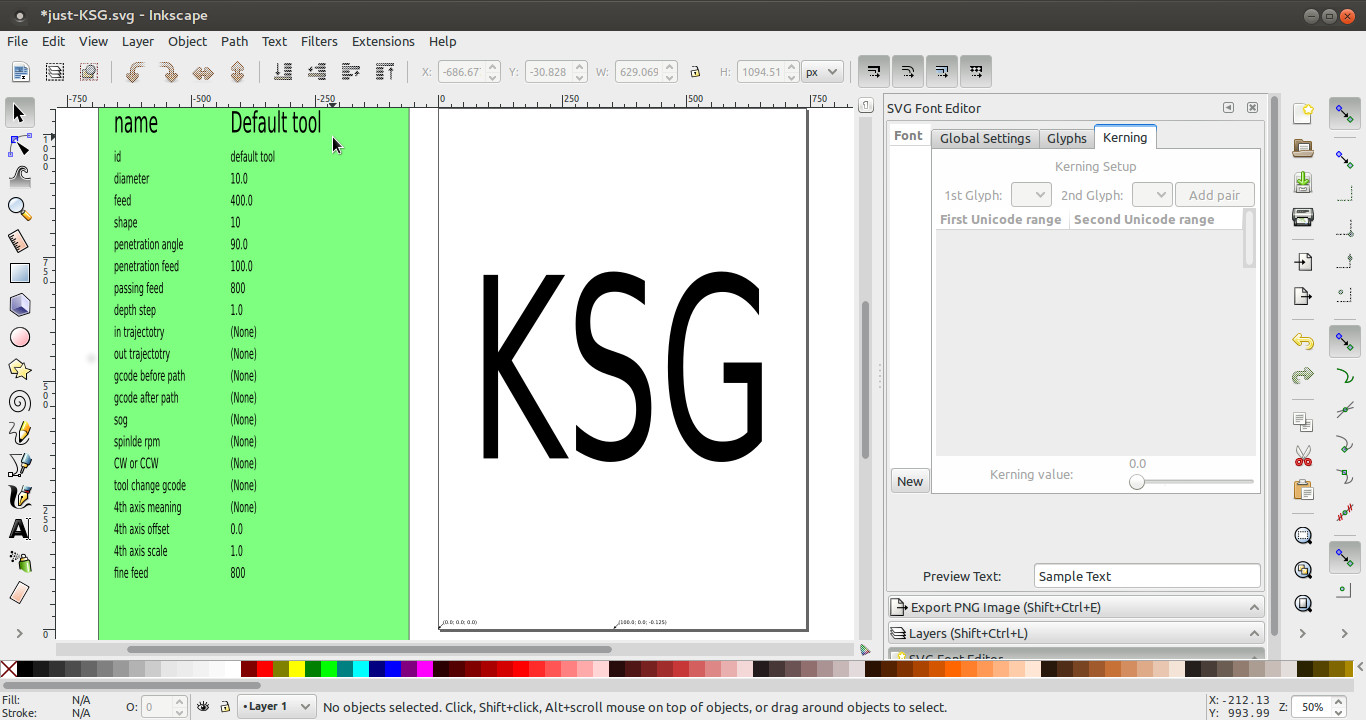
\includegraphics[width=1.3\textwidth]{./07-images/img-Ch4App/Inkscape-Display-of-2D-KSG.jpg}}
		\caption{App4-Inkscape display of 2D KSG jpg file.}
		\label{fig:App4-Inkscape-Display-of-2D-KSG.jpg}
	\end{center}
\end{figure}

% ========================================================
\pagebreak
\textbf{Display Text for 2D KSG model SVG/XML (Clipped text from 671 lines total)}

% ==========================================================
\lstset{basicstyle=\footnotesize, numberstyle=\tiny\color{blue}, frame=single, numbers=left, firstnumber=1, stepnumber=1, numbersep=1pt, xleftmargin=2.0em, framexleftmargin=1.5em, xrightmargin=0.0em, breaklines=true, breakatwhitespace=false, breakindent=5pt, prebreak=\space, postbreak=\space }
% ==========================================================

\begin{lstlisting}[caption={App4-Display Text for 2D KSG model SVG/XML}, label=App4-Display Text for 2D KSG model SVG/XML]
<?xml version="1.0" encoding="UTF-8" standalone="no"?>
<!-- Created with Inkscape (http://www.inkscape.org/) -->

<svg
xmlns:dc="http://purl.org/dc/elements/1.1/"
xmlns:cc="http://creativecommons.org/ns#"
xmlns:rdf="http://www.w3.org/1999/02/22-rdf-syntax-ns#"
xmlns:svg="http://www.w3.org/2000/svg"
xmlns="http://www.w3.org/2000/svg"
xmlns:sodipodi="http://sodipodi.sourceforge.net/DTD/sodipodi-0.dtd"
xmlns:inkscape="http://www.inkscape.org/namespaces/inkscape"
	width="210mm"
	height="297mm"
	viewBox="0 0 744.09448819 1052.3622047"
	id="svg4749"
	version="1.1"
	inkscape:version="0.91 r13725"
	sodipodi:docname="just-KSG.svg">
	<sodipodi:namedview
	id="base"
	pagecolor="#ffffff"
	bordercolor="#666666"
	borderopacity="1.0"
	inkscape:pageopacity="0.0"
	inkscape:pageshadow="2"
	inkscape:zoom="0.35"
	inkscape:cx="375"
	inkscape:cy="520"
	inkscape:document-units="px"
	inkscape:current-layer="layer1"
	showgrid="false"
	inkscape:window-width="1366"
	inkscape:window-height="689"
	inkscape:window-x="0"
	inkscape:window-y="24"
	inkscape:window-maximized="1" />
	<defs
	id="defs4751" />
	<metadata
	id="metadata4754">
	<rdf:RDF>
	<cc:Work
	rdf:about="">
	<dc:format>image/svg+xml</dc:format>
	<dc:type
	rdf:resource="http://purl.org/dc/dcmitype/StillImage" />
	<dc:title></dc:title>
	</cc:Work>
	</rdf:RDF>
	</metadata>
	<g
	id="layer1"
	inkscape:groupmode="layer"
	inkscape:label="Layer 1">
	<text
	transform="scale(0.76565133,1.3060775)"
	sodipodi:linespacing="125%"
	id="text4757"
	y="554.98346"
	x="81.874046"
	style="font-style:normal;font-weight:normal;font-size:389.44628906px;line-height:125%;font-family:sans-serif;letter-spacing:0px;word-spacing:0px;fill:#000000;fill-opacity:1;stroke:none;stroke-width:1px;stroke-linecap:butt;stroke-linejoin:miter;stroke-opacity:1"
	xml:space="preserve"><tspan
	y="554.98346"
	x="81.874046"
	id="tspan4759"
	sodipodi:role="line">KSG</tspan></text>
	<g
	id="g4787"
	gcodetools="Gcodetools orientation group">
	<g
	id="g4789"
	gcodetools="Gcodetools orientation point (2 points)">
	<path
	id="path4791"
	style="stroke:none;fill:#000000;"
	gcodetools="Gcodetools orientation point arrow"
	d="m 0.0,1052.36220472 2.9375,-6.343750000001 0.8125,1.90625 6.843748640396,-6.84374864039 0,0 0.6875,0.6875 -6.84375,6.84375 1.90625,0.812500000001 z z" />
	<text
	id="text4793"
	xml:space="preserve"
	y="1042.36220472"
	x="10.0"
	style="font-family:DejaVu Sans;font-style:normal;font-variant:normal;font-weight:normal;font-stretch:normal;font-family:DejaVu Sans;fill:#000000;fill-opacity:1;stroke:none;font-size:10.000000px;"
	gcodetools="Gcodetools orientation point text"><tspan
	id="tspan4795"
	sodipodi:role="line"
	y="1042.36220472"
	x="10.0">(0.0; 0.0; 0.0)</tspan></text>
	</g>

.... BEGIN CLIPPED TEXT
....
.... END CLIPPED TEXT
        x="150"
       style="font-style:normal;font-variant:normal;font-weight:normal;font-stretch:normal;font-size:10px;font-family:'DejaVu Sans';fill:#000000;fill-opacity:1;stroke:none"
       gcodetools="Gcodetools tool definition field value"><tspan
       id="tspan5017"
       sodipodi:role="line"
       y="305"
       x="150">800</tspan></text>
       </g>
       </g>
       </g>
       <g
       id="g5019" />
</svg>
THE END AT LINE 671      
\end{lstlisting}
% ===========================================================


\pagebreak
\clearpage
%===========================================================

% =========================================================
\subsection{App4-Creation of G-Code for 2D Model}\label{sec:App4-Creation of G-Code for 2D Model}
% =========================================================

\begin{enumerate}
	%%\vspace{0.2cm}
	
\item \textbf{CAM software tracing 2D model KSG drawing}

To convert the model into G-Code, some software tool, like CAM, must trace the 2D model drawing (SVG or STL) for lines, curves and surfaces, then capture and save those point traces as numerical data into a file. These points saved into the file are only geometrical points. There are no instruction commands for a CNC machine to follow inside this file.

\item \textbf{CAM software added machining instructions to make G-Code}

The next step for CAM, is to read the numerical data file, determine how a machine should trace the geometrical codes, and add these machine instructions into the data file. Now the file becomes a G-code file. 

This CAM file trace includes not only captures of the points as numerical path data (G series), but also CNC tool movements like speeds (F series) to move along the data points as well as associated CNC tool jumps from point-to-point. In addition, CNC service commands are also added into the G-Code file, like (M series) to start and stop the tool, to start and stop lubrication fluids, to pause and change tool cutters, and so on. 
 
Typically, the (G00, G01. G02 and G03) are the primary movement commands generated in conversion from models to G-Code files.

Note that, a CAD model drawing file only contains path data and geometric elements. It does not contain CNC machine movements and other machine service instructions.
 
% \vspace{0.2cm}
\item \textbf{Intensive CAM software computations to produce G-Code}

% \vspace{0.2cm}
Just consider a simple 2D model of the letters "KSG" as we have shown in the previous section. For that, the CAM engine must process about 700 lines of SVG text codes to produce the G-Code file. Imagine, for very large and complex 2D and 3D model drawings, for example, large SVG, STL files. The conversion of these model drawings to G-Code can be very time consuming, like hours to complete. And the resulting G-Code files can run into thousands of G-Code command lines. 
vspace{0.2cm}

A single command instruction in G-Code file is usually written as a one line entry. This varies depending on the G-Codes standard in practice. Because of efficient curve interpolation, NURBS entries in G-Code like G06 series, make the overall G-Code file size smaller. However, NURBS G-Code entries are generally more complicated to interpret and execute by the CNC Interpreter and CNC Interpolator software, compared to common G01, G02 and G03 codes. High end FANUC CNC machines implement NURBS interpolation and they have their own software (proprietary) to accomplish that.
\vspace{0.2cm}

In our illustration example, the KSG 2D drawing is simple, and only contains linear and arc elements with an SVG file consisting of about 700 lines. This number varies depending on software graphic applications and their vector format. For this drawing, we generated a G-Code file in RS274D NGC format with just 200 lines. This file does not contain NURBS G-Codes.
\vspace{0.2cm}

An excerpt showing typical motion commands like G00, G01, G02 and G03 in G-Code for the KSG 2D model can be seen following that at Listing \ref{App4-Display excerpt listing for 2D KSG G-Code} .

The full textual contents of the G-Code generated file for our KSG 2D model drawing can be seen in the next section at Listing \ref{App4-Display full listing for 2D KSG G-Code} . 

\end{enumerate}

\textbf{Display excerpt listing for 2D KSG G-Code}
\vspace{0.3cm}

Notice that from lines no. 27 until line no. 51 in this excerpt, we can see typical motion commands like G00, G01, G02 and G03 in G-Code. 

% ==========================================================
\lstset{basicstyle=\footnotesize, numberstyle=\tiny\color{blue}, frame=single, numbers=left, firstnumber=1, stepnumber=1, numbersep=1pt, xleftmargin=2.0em, framexleftmargin=1.5em, xrightmargin=0.0em, breaklines=true, breakatwhitespace=false, breakindent=5pt, prebreak=\space, postbreak=\space }
% ==========================================================

\begin{lstlisting}[caption={App4-Display excerpt listing for 2D KSG G-Code}, label=App4-Display excerpt listing for 2D KSG G-Code]
%
(Header)
(Generated by gcodetools from Inkscape.)
(Using default header. To add your own header create file "header" in the output dir.)
M3
(Header end.)
G21 (All units in mm)
#8  = 0 (Z axis offset)
#6  = 0 (X axis offset)
#7  = 0 (Y axis offset)
#10 = 1 (XY Scale factor)
#11 = 1 (Z Scale factor)
#21 = 400.000000 (Feed definition)
#20 = 100.000000 (Feed definition)

(Start cutting path id: path5167)
(Change tool to Default tool)

.... CLIPPED SECTION ----

(Start cutting path id: path5165)
(Change tool to Default tool)

G00 Z[5.000000*#11+#8]
G00 X[117.952117*#10+#6] Y[193.645846*#10+#7]

G01 Z[1.000000*#11+#8] F [#20](Penetrate)
G01 X[117.952117*#10+#6] Y[179.837424*#10+#7] Z[1.000000*#11+#8] F [#21]
G03 X[113.046989*#10+#6] Y[183.402174*#10+#7] Z[1.000000*#11+#8] I[-34.318323*#10] J[-42.065200*#10]
G03 X[109.035511*#10+#6] Y[185.585093*#10+#7] Z[1.000000*#11+#8] I[-16.685118*#10] J[-25.884338*#10]
G03 X[104.749703*#10+#6] Y[187.038280*#10+#7] Z[1.000000*#11+#8] I[-9.591941*#10] J[-21.242475*#10]
G03 X[100.940711*#10+#6] Y[187.477618*#10+#7] Z[1.000000*#11+#8] I[-3.808992*#10] J[-16.292016*#10]
G03 X[94.758678*#10+#6] Y[186.209903*#10+#7] Z[1.000000*#11+#8] I[-0.000000*#10] J[-15.707261*#10]
G03 X[90.462671*#10+#6] Y[182.991632*#10+#7] Z[1.000000*#11+#8] I[4.472674*#10] J[-10.446948*#10]
G03 X[87.912396*#10+#6] Y[178.111685*#10+#7] Z[1.000000*#11+#8] I[10.615970*#10] J[-8.654302*#10]
G03 X[86.805629*#10+#6] Y[170.234616*#10+#7] Z[1.000000*#11+#8] I[27.477917*#10] J[-7.877068*#10]
G03 X[87.568633*#10+#6] Y[163.529681*#10+#7] Z[1.000000*#11+#8] I[29.841487*#10] J[0.000000*#10]
G03 X[89.229960*#10+#6] Y[159.720590*#10+#7] Z[1.000000*#11+#8] I[11.027232*#10] J[2.542666*#10]
G03 X[92.213942*#10+#6] Y[156.922563*#10+#7] Z[1.000000*#11+#8] I[8.237512*#10] J[5.794811*#10]
G03 X[98.516380*#10+#6] Y[154.043014*#10+#7] Z[1.000000*#11+#8] I[15.074024*#10] J[24.655545*#10]
G01 X[103.529404*#10+#6] Y[152.290678*#10+#7] Z[1.000000*#11+#8]
G02 X[111.731935*#10+#6] Y[147.939660*#10+#7] Z[1.000000*#11+#8] I[-8.284484*#10] J[-25.525105*#10]
G02 X[117.212491*#10+#6] Y[141.636464*#10+#7] Z[1.000000*#11+#8] I[-13.341928*#10] J[-17.134888*#10]
G02 X[120.313088*#10+#6] Y[133.703323*#10+#7] Z[1.000000*#11+#8] I[-23.402927*#10] J[-13.719316*#10]
G02 X[121.650249*#10+#6] Y[121.309349*#10+#7] Z[1.000000*#11+#8] I[-56.770488*#10] J[-12.393974*#10]
G02 X[119.784929*#10+#6] Y[106.730189*#10+#7] Z[1.000000*#11+#8] I[-57.907303*#10] J[-0.000000*#10]
G02 X[115.651058*#10+#6] Y[98.248584*#10+#7] Z[1.000000*#11+#8] I[-23.094899*#10] J[6.008071*#10]
G02 X[108.584210*#10+#6] Y[92.631505*#10+#7] Z[1.000000*#11+#8] I[-14.532534*#10] J[11.029440*#10]
G02 X[98.146568*#10+#6] Y[90.398113*#10+#7] Z[1.000000*#11+#8] I[-10.437642*#10] J[23.273202*#10]
G02 X[93.854953*#10+#6] Y[90.783690*#10+#7] Z[1.000000*#11+#8] I[-0.000000*#10] J[24.076414*#10]
G02 X[88.860148*#10+#6] Y[92.080356*#10+#7] Z[1.000000*#11+#8] I[6.155305*#10] J[33.978893*#10]

--- CLIPPED SECTION ----

(Footer)
M5
G00 X0.0000 Y0.0000
M2
(Using default footer. To add your own footer create file "footer" in the output dir.)
(end)
%
\end{lstlisting}

% ==========================================================
\pagebreak
\textbf{Display full listing for 2D KSG G-Code}
\vspace{0.3cm}

% ==========================================================
\lstset{basicstyle=\footnotesize, numberstyle=\tiny\color{blue}, frame=single, numbers=left, firstnumber=1, stepnumber=1, numbersep=1pt, xleftmargin=2.0em, framexleftmargin=1.5em, xrightmargin=0.0em, breaklines=true, breakatwhitespace=false, breakindent=5pt, prebreak=\space, postbreak=\space }
% ==========================================================

\begin{lstlisting}[caption={App4-Display full listing for 2D KSG G-Code}, label=App4-Display full listing for 2D KSG G-Code]
%
(Header)
(Generated by gcodetools from Inkscape.)
(Using default header. To add your own header create file "header" in the output dir.)
M3
(Header end.)
G21 (All units in mm)
#8  = 0 (Z axis offset)
#6  = 0 (X axis offset)
#7  = 0 (Y axis offset)
#10 = 1 (XY Scale factor)
#11 = 1 (Z Scale factor)
#21 = 400.000000 (Feed definition)
#20 = 100.000000 (Feed definition)

(Start cutting path id: path5167)
(Change tool to Default tool)

G00 Z[5.000000*#11+#8]
G00 X[176.423691*#10+#6] Y[107.360743*#10+#7]

G01 Z[1.000000*#11+#8] F [#20](Penetrate)
G01 X[176.423691*#10+#6] Y[135.468236*#10+#7] Z[1.000000*#11+#8] F [#21]
G01 X[162.863873*#10+#6] Y[135.468236*#10+#7] Z[1.000000*#11+#8]
G01 X[162.863873*#10+#6] Y[147.103758*#10+#7] Z[1.000000*#11+#8]
G01 X[184.641760*#10+#6] Y[147.103758*#10+#7] Z[1.000000*#11+#8]
G01 X[184.641760*#10+#6] Y[102.173824*#10+#7] Z[1.000000*#11+#8]
G02 X[179.391923*#10+#6] Y[96.903039*#10+#7] Z[1.000000*#11+#8] I[-30.942596*#10] J[25.569747*#10]
G02 X[174.040450*#10+#6] Y[93.342040*#10+#7] Z[1.000000*#11+#8] I[-19.182522*#10] J[23.025911*#10]
G02 X[168.066958*#10+#6] Y[91.148675*#10+#7] Z[1.000000*#11+#8] I[-12.219785*#10] J[24.048923*#10]
G02 X[161.672253*#10+#6] Y[90.398113*#10+#7] Z[1.000000*#11+#8] I[-6.394705*#10] J[26.865808*#10]
G02 X[149.370262*#10+#6] Y[93.974078*#10+#7] Z[1.000000*#11+#8] I[-0.000000*#10] J[22.948566*#10]
G02 X[139.154740*#10+#6] Y[104.697188*#10+#7] Z[1.000000*#11+#8] I[16.440628*#10] J[25.889933*#10]
G02 X[133.559873*#10+#6] Y[119.722073*#10+#7] Z[1.000000*#11+#8] I[44.792682*#10] J[25.233731*#10]
G02 X[131.059941*#10+#6] Y[144.650484*#10+#7] Z[1.000000*#11+#8] I[123.038549*#10] J[24.928411*#10]
G02 X[133.566449*#10+#6] Y[169.644463*#10+#7] Z[1.000000*#11+#8] I[125.868687*#10] J[0.000000*#10]
G02 X[139.154740*#10+#6] Y[184.603785*#10+#7] Z[1.000000*#11+#8] I[49.856648*#10] J[-10.101281*#10]
G02 X[149.381921*#10+#6] Y[195.385610*#10+#7] Z[1.000000*#11+#8] I[26.785332*#10] J[-15.165982*#10]
G02 X[161.672253*#10+#6] Y[198.972953*#10+#7] Z[1.000000*#11+#8] I[12.290332*#10] J[-19.259830*#10]
G02 X[167.528571*#10+#6] Y[198.331573*#10+#7] Z[1.000000*#11+#8] I[0.000000*#10] J[-27.057176*#10]
G02 X[173.054281*#10+#6] Y[196.449585*#10+#7] Z[1.000000*#11+#8] I[-5.749598*#10] J[-25.934418*#10]
G02 X[178.118029*#10+#6] Y[193.430835*#10+#7] Z[1.000000*#11+#8] I[-12.194513*#10] J[-26.211890*#10]
G02 X[183.039237*#10+#6] Y[189.019673*#10+#7] Z[1.000000*#11+#8] I[-21.688851*#10] J[-29.147349*#10]
G01 X[183.039237*#10+#6] Y[173.949571*#10+#7] Z[1.000000*#11+#8]
G03 X[177.959907*#10+#6] Y[180.117456*#10+#7] Z[1.000000*#11+#8] I[-39.092615*#10] J[-27.017866*#10]
G03 X[173.259733*#10+#6] Y[183.972941*#10+#7] Z[1.000000*#11+#8] I[-19.689245*#10] J[-19.210212*#10]
G03 X[167.837734*#10+#6] Y[186.512086*#10+#7] Z[1.000000*#11+#8] I[-11.832629*#10] J[-18.208427*#10]
G03 X[162.370790*#10+#6] Y[187.337430*#10+#7] Z[1.000000*#11+#8] I[-5.466944*#10] J[-17.693398*#10]
G03 X[152.786893*#10+#6] Y[184.557277*#10+#7] Z[1.000000*#11+#8] I[0.000000*#10] J[-17.909143*#10]
G03 X[145.441564*#10+#6] Y[176.613122*#10+#7] Z[1.000000*#11+#8] I[11.266522*#10] J[-17.785156*#10]
G03 X[141.629050*#10+#6] Y[165.440943*#10+#7] Z[1.000000*#11+#8] I[33.955998*#10] J[-17.824110*#10]
G03 X[139.812185*#10+#6] Y[144.650484*#10+#7] Z[1.000000*#11+#8] I[118.044621*#10] J[-20.790459*#10]
G03 X[141.626890*#10+#6] Y[123.929590*#10+#7] Z[1.000000*#11+#8] I[119.206343*#10] J[-0.000000*#10]
G03 X[145.441564*#10+#6] Y[112.757940*#10+#7] Z[1.000000*#11+#8] I[37.812227*#10] J[6.674267*#10]
G03 X[152.786892*#10+#6] Y[104.813789*#10+#7] Z[1.000000*#11+#8] I[18.611844*#10] J[9.841002*#10]
G03 X[162.370790*#10+#6] Y[102.033636*#10+#7] Z[1.000000*#11+#8] I[9.583897*#10] J[15.128996*#10]
G03 X[166.706157*#10+#6] Y[102.379890*#10+#7] Z[1.000000*#11+#8] I[0.000000*#10] J[27.314245*#10]
G03 X[170.219047*#10+#6] Y[103.295320*#10+#7] Z[1.000000*#11+#8] I[-3.020477*#10] J[18.788763*#10]
G03 X[173.456867*#10+#6] Y[104.956924*#10+#7] Z[1.000000*#11+#8] I[-6.197101*#10] J[16.061169*#10]
G03 X[176.423691*#10+#6] Y[107.360743*#10+#7] Z[1.000000*#11+#8] I[-10.386640*#10] J[15.852077*#10]
G01 X[176.423691*#10+#6] Y[107.360743*#10+#7] Z[1.000000*#11+#8]
G00 Z[5.000000*#11+#8]

(End cutting path id: path5167)

(Start cutting path id: path5165)
(Change tool to Default tool)

G00 Z[5.000000*#11+#8]
G00 X[117.952117*#10+#6] Y[193.645846*#10+#7]

G01 Z[1.000000*#11+#8] F [#20](Penetrate)
G01 X[117.952117*#10+#6] Y[179.837424*#10+#7] Z[1.000000*#11+#8] F [#21]
G03 X[113.046989*#10+#6] Y[183.402174*#10+#7] Z[1.000000*#11+#8] I[-34.318323*#10] J[-42.065200*#10]
G03 X[109.035511*#10+#6] Y[185.585093*#10+#7] Z[1.000000*#11+#8] I[-16.685118*#10] J[-25.884338*#10]
G03 X[104.749703*#10+#6] Y[187.038280*#10+#7] Z[1.000000*#11+#8] I[-9.591941*#10] J[-21.242475*#10]
G03 X[100.940711*#10+#6] Y[187.477618*#10+#7] Z[1.000000*#11+#8] I[-3.808992*#10] J[-16.292016*#10]
G03 X[94.758678*#10+#6] Y[186.209903*#10+#7] Z[1.000000*#11+#8] I[-0.000000*#10] J[-15.707261*#10]
G03 X[90.462671*#10+#6] Y[182.991632*#10+#7] Z[1.000000*#11+#8] I[4.472674*#10] J[-10.446948*#10]
G03 X[87.912396*#10+#6] Y[178.111685*#10+#7] Z[1.000000*#11+#8] I[10.615970*#10] J[-8.654302*#10]
G03 X[86.805629*#10+#6] Y[170.234616*#10+#7] Z[1.000000*#11+#8] I[27.477917*#10] J[-7.877068*#10]
G03 X[87.568633*#10+#6] Y[163.529681*#10+#7] Z[1.000000*#11+#8] I[29.841487*#10] J[0.000000*#10]
G03 X[89.229960*#10+#6] Y[159.720590*#10+#7] Z[1.000000*#11+#8] I[11.027232*#10] J[2.542666*#10]
G03 X[92.213942*#10+#6] Y[156.922563*#10+#7] Z[1.000000*#11+#8] I[8.237512*#10] J[5.794811*#10]
G03 X[98.516380*#10+#6] Y[154.043014*#10+#7] Z[1.000000*#11+#8] I[15.074024*#10] J[24.655545*#10]
G01 X[103.529404*#10+#6] Y[152.290678*#10+#7] Z[1.000000*#11+#8]
G02 X[111.731935*#10+#6] Y[147.939660*#10+#7] Z[1.000000*#11+#8] I[-8.284484*#10] J[-25.525105*#10]
G02 X[117.212491*#10+#6] Y[141.636464*#10+#7] Z[1.000000*#11+#8] I[-13.341928*#10] J[-17.134888*#10]
G02 X[120.313088*#10+#6] Y[133.703323*#10+#7] Z[1.000000*#11+#8] I[-23.402927*#10] J[-13.719316*#10]
G02 X[121.650249*#10+#6] Y[121.309349*#10+#7] Z[1.000000*#11+#8] I[-56.770488*#10] J[-12.393974*#10]
G02 X[119.784929*#10+#6] Y[106.730189*#10+#7] Z[1.000000*#11+#8] I[-57.907303*#10] J[-0.000000*#10]
G02 X[115.651058*#10+#6] Y[98.248584*#10+#7] Z[1.000000*#11+#8] I[-23.094899*#10] J[6.008071*#10]
G02 X[108.584210*#10+#6] Y[92.631505*#10+#7] Z[1.000000*#11+#8] I[-14.532534*#10] J[11.029440*#10]
G02 X[98.146568*#10+#6] Y[90.398113*#10+#7] Z[1.000000*#11+#8] I[-10.437642*#10] J[23.273202*#10]
G02 X[93.854953*#10+#6] Y[90.783690*#10+#7] Z[1.000000*#11+#8] I[-0.000000*#10] J[24.076414*#10]
G02 X[88.860148*#10+#6] Y[92.080356*#10+#7] Z[1.000000*#11+#8] I[6.155305*#10] J[33.978893*#10]
G02 X[84.109236*#10+#6] Y[94.053384*#10+#7] Z[1.000000*#11+#8] I[13.446482*#10] J[39.084622*#10]
G02 X[78.710831*#10+#6] Y[97.056998*#10+#7] Z[1.000000*#11+#8] I[26.242970*#10] J[53.519667*#10]
G01 X[78.710831*#10+#6] Y[111.636444*#10+#7] Z[1.000000*#11+#8]
G03 X[84.025978*#10+#6] Y[107.168820*#10+#7] Z[1.000000*#11+#8] I[37.287981*#10] J[38.966103*#10]
G03 X[88.613605*#10+#6] Y[104.346723*#10+#7] Z[1.000000*#11+#8] I[19.239604*#10] J[26.136178*#10]
G03 X[93.599617*#10+#6] Y[102.469141*#10+#7] Z[1.000000*#11+#8] I[11.130303*#10] J[21.997980*#10]
G03 X[98.146568*#10+#6] Y[101.893449*#10+#7] Z[1.000000*#11+#8] I[4.546951*#10] J[17.668599*#10]
G03 X[104.614313*#10+#6] Y[103.237701*#10+#7] Z[1.000000*#11+#8] I[-0.000000*#10] J[16.231605*#10]
G03 X[109.117692*#10+#6] Y[106.659805*#10+#7] Z[1.000000*#11+#8] I[-4.741455*#10] J[10.913805*#10]
G03 X[111.808038*#10+#6] Y[111.841476*#10+#7] Z[1.000000*#11+#8] I[-11.297040*#10] J[9.154726*#10]
G03 X[112.980184*#10+#6] Y[120.257946*#10+#7] Z[1.000000*#11+#8] I[-29.630701*#10] J[8.416470*#10]
G03 X[112.127054*#10+#6] Y[127.717636*#10+#7] Z[1.000000*#11+#8] I[-33.039967*#10] J[0.000000*#10]
G03 X[110.186041*#10+#6] Y[132.314028*#10+#7] Z[1.000000*#11+#8] I[-14.213271*#10] J[-3.294098*#10]
G03 X[106.818823*#10+#6] Y[135.882125*#10+#7] Z[1.000000*#11+#8] I[-10.873106*#10] J[-6.888092*#10]
G03 X[101.105073*#10+#6] Y[138.832725*#10+#7] Z[1.000000*#11+#8] I[-12.895623*#10] J[-17.964440*#10]
G01 X[96.050959*#10+#6] Y[140.514968*#10+#7] Z[1.000000*#11+#8]
G02 X[87.715741*#10+#6] Y[144.862945*#10+#7] Z[1.000000*#11+#8] I[9.895237*#10] J[29.132934*#10]
G02 X[82.614413*#10+#6] Y[150.398154*#10+#7] Z[1.000000*#11+#8] I[11.687787*#10] J[15.889965*#10]
G02 X[79.737752*#10+#6] Y[157.488256*#10+#7] Z[1.000000*#11+#8] I[19.564586*#10] J[12.066546*#10]
G02 X[78.464288*#10+#6] Y[169.113120*#10+#7] Z[1.000000*#11+#8] I[52.422259*#10] J[11.624864*#10]
G02 X[80.176218*#10+#6] Y[182.442710*#10+#7] Z[1.000000*#11+#8] I[52.750021*#10] J[0.000000*#10]
G02 X[84.175848*#10+#6] Y[190.982294*#10+#7] Z[1.000000*#11+#8] I[25.128284*#10] J[-6.562740*#10]
G02 X[91.023399*#10+#6] Y[196.835582*#10+#7] Z[1.000000*#11+#8] I[15.406407*#10] J[-11.091406*#10]
G02 X[99.995634*#10+#6] Y[198.972953*#10+#7] Z[1.000000*#11+#8] I[8.972235*#10] J[-17.763096*#10]
G02 X[104.263355*#10+#6] Y[198.651605*#10+#7] Z[1.000000*#11+#8] I[-0.000000*#10] J[-28.499848*#10]
G02 X[108.788968*#10+#6] Y[197.641175*#10+#7] Z[1.000000*#11+#8] I[-5.009916*#10] J[-33.078997*#10]
G02 X[113.155807*#10+#6] Y[196.046682*#10+#7] Z[1.000000*#11+#8] I[-10.854275*#10] J[-36.503587*#10]
G02 X[117.952117*#10+#6] Y[193.645846*#10+#7] Z[1.000000*#11+#8] I[-20.261739*#10] J[-46.469596*#10]
G01 X[117.952117*#10+#6] Y[193.645846*#10+#7] Z[1.000000*#11+#8]
G00 Z[5.000000*#11+#8]

(End cutting path id: path5165)

(Start cutting path id: path5163)
(Change tool to Default tool)

G00 Z[5.000000*#11+#8]
G00 X[25.950818*#10+#6] Y[197.080429*#10+#7]

G01 Z[1.000000*#11+#8] F [#20](Penetrate)
G01 X[34.251068*#10+#6] Y[197.080429*#10+#7] Z[1.000000*#11+#8] F [#21]
G01 X[34.251068*#10+#6] Y[152.851428*#10+#7] Z[1.000000*#11+#8]
G01 X[61.781606*#10+#6] Y[197.080429*#10+#7] Z[1.000000*#11+#8]
G01 X[72.465097*#10+#6] Y[197.080429*#10+#7] Z[1.000000*#11+#8]
G01 X[42.017145*#10+#6] Y[148.295349*#10+#7] Z[1.000000*#11+#8]
G01 X[74.642884*#10+#6] Y[92.430825*#10+#7] Z[1.000000*#11+#8]
G01 X[63.712853*#10+#6] Y[92.430825*#10+#7] Z[1.000000*#11+#8]
G01 X[34.251068*#10+#6] Y[142.828054*#10+#7] Z[1.000000*#11+#8]
G01 X[34.251068*#10+#6] Y[92.430825*#10+#7] Z[1.000000*#11+#8]
G01 X[25.950818*#10+#6] Y[92.430825*#10+#7] Z[1.000000*#11+#8]
G01 X[25.950818*#10+#6] Y[197.080429*#10+#7] Z[1.000000*#11+#8]
G01 X[25.950818*#10+#6] Y[197.080429*#10+#7] Z[1.000000*#11+#8]
G00 Z[5.000000*#11+#8]

(End cutting path id: path5163)

(Footer)
M5
G00 X0.0000 Y0.0000
M2

(Using default footer. To add your own footer create file "footer" in the output dir.)
(end)
%
\end{lstlisting}

%% =========================================================



\pagebreak
\clearpage
%% END LANDSCAPE ENTIRELY
\end{landscape}
\end{flushleft}
%% ========= END Chapter-4 Appendices ===================== %% Related Research Work
	% ==========================================================
\clearpage
\pagebreak
\justifying
\renewcommand{\thesection}{E \arabic{section}}

\titleformat{\section}{\normalfont\LARGE\bfseries\color{black}}{\thesection}{10pt}{\LARGE}
\section{Appendix-E5 Research Implementation Plan}\label{sec:App5-Research-Implementation-Plan}

%============================================================
\subsection{App5-PhD Proposal Document Preparation}
\begin{figure}[htbp]
	\begin{center}
		\frame{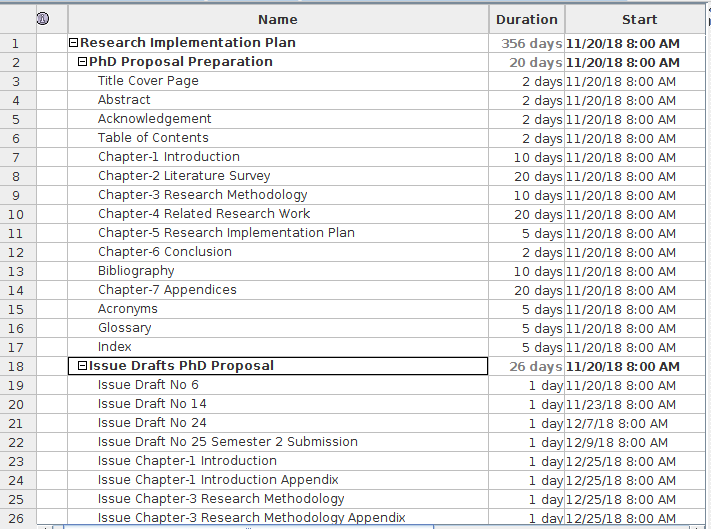
\includegraphics[width=1.00\textwidth]{./07-images/img-Ch5App/01-Research-Implementation-Plan.png}}
		\caption{App5-PhD Proposal Document Preparation}
		\label{fig:App5-01-Research-Implementation-Plan.png}
	\end{center}
\end{figure}

Note that the contents of a proposal document do not include the chapter on implementation design and the chapter on results and discussion, which are both required for a thesis document.

	
\pagebreak	
\subsection{App5-Procurement of Long Lead Items and Project Setup}
\begin{figure}[htbp]
	\begin{center}
		\frame{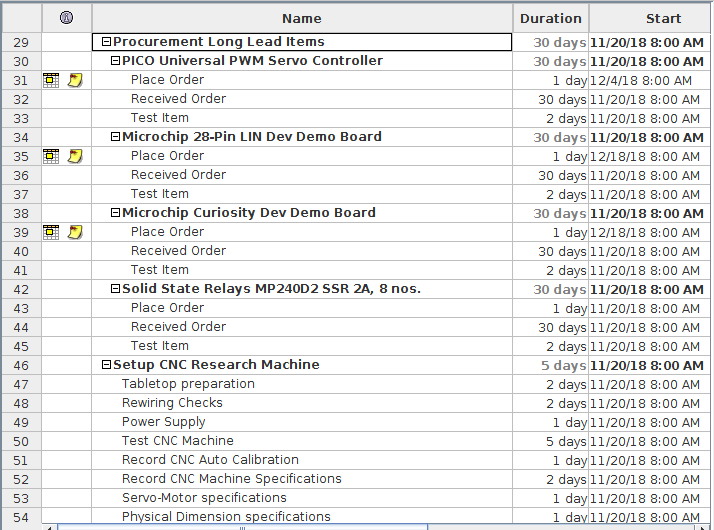
\includegraphics[width=1.00\textwidth]{./07-images/img-Ch5App/02-Research-Implementation-Plan.png}}
		\caption{App5-Procurement of Long Lead Items and Project Setup}
		\label{fig:App5-02-Research-Implementation-Plan.png}
	\end{center}
\end{figure}

The long lead items above are hardware resources that must be procured for the project.

\pagebreak
\subsection{App5-Computer 64bit Resources and Software Installations}
\begin{figure}[htbp]
	\begin{center}
		\frame{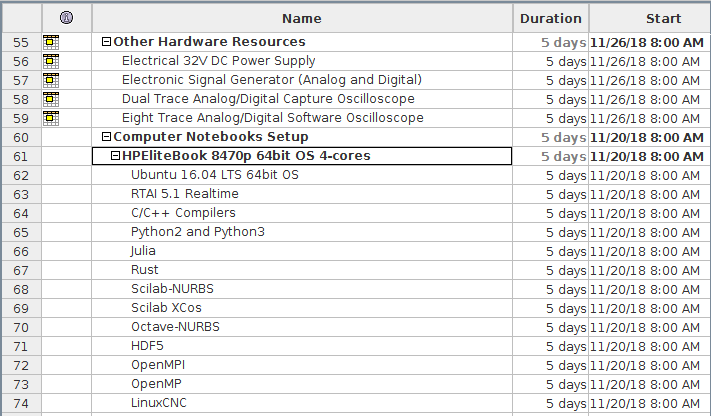
\includegraphics[width=1.00\textwidth]{./07-images/img-Ch5App/03-Research-Implementation-Plan.png}}
		\caption{App5-Computer 64bit Resources and Software Installations}
		\label{fig:App5-03-Research-Implementation-Plan.png}
	\end{center}
\end{figure}

We will be implementing the CNC Control software on both 64bit and 32bit systems. The Linux kernel for the 64bit system is of version 4.X, while that for the 32bit system is of version 3.X. The Realtime RTAI library for the 64bit system is of version 5.1, while that for the 32bit system is version 2.7.  
\vspace{0.5cm}

The above tasks in the figure identify the 64bit hardware resources and their associated software that are required for the project.

\pagebreak
\subsection{App5-Computer 32bit Resources and Software Installations}
\begin{figure}[htbp]
	\begin{center}
		\frame{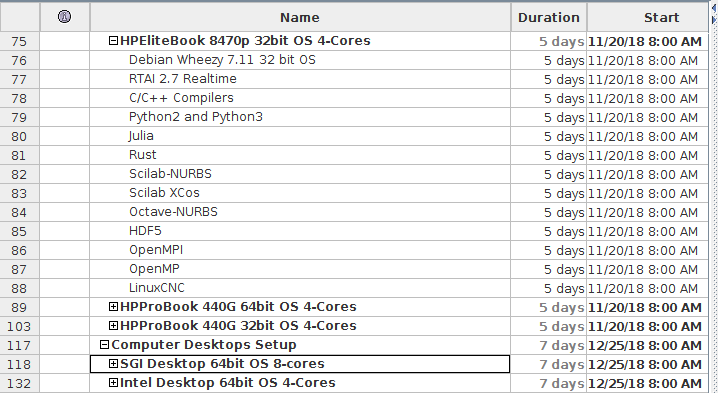
\includegraphics[width=1.00\textwidth]{./07-images/img-Ch5App/04-Research-Implementation-Plan.png}}
		\caption{App5-Computer 32bit Resources and Software Installations}
		\label{fig:App5-04-Research-Implementation-Plan.png}
	\end{center}
\end{figure}

We will be implementing the CNC Control software on four(4) different computer hardware configurations (number of CPU cores, memory speeds, hard disk speeds, etc) for the purposes of performance comparisons. The multi-core feature of the computers is for true parallel computation design. The different computers are as follows:

\begin{enumerate}
	\item Notebook HP EliteBook 8470p, 4-cores, installed with both 64bit and 32bit Linux operating systems.   
	
	\item Notebook HP ProBook 440G, 4-cores, installed with both 64bit and 32bit Linux operating systems.
	
	\item Desktop SGI, 8-cores, installed with only 64bit Linux operating system. Does not accept 32bit OS.
	
	\item Desktop Intel, 4-cores, installed with both 64bit and 32bit Linux operating systems.
\end{enumerate}

The above tasks in the figure identify the 32bit hardware resources and their associated software that are required for the project.

\pagebreak
\subsection{App5-UseCase Design and Software Architecture Design}\label{sec:App5-UseCase Design}
\begin{figure}[htbp]
	\begin{center}
		\frame{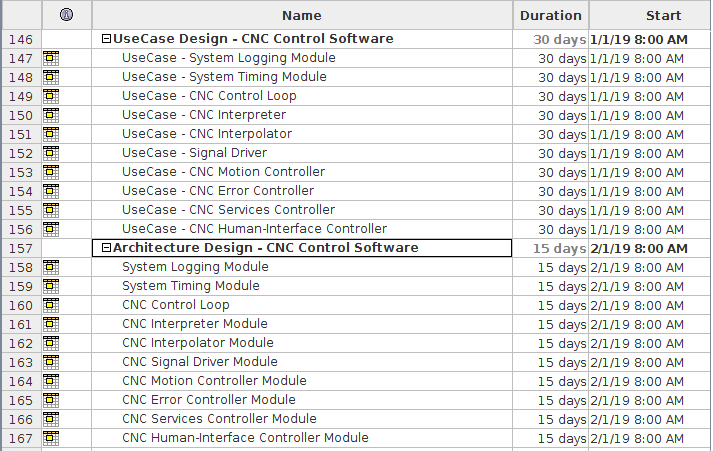
\includegraphics[width=1.00\textwidth]{./07-images/img-Ch5App/05-Research-Implementation-Plan.png}}
		\caption{App5-UseCase Design and Software Architecture Design}
		\label{fig:App5-05-Research-Implementation-Plan.png}
	\end{center}
\end{figure}


\pagebreak	
\subsection{App5-Process and Data Flow Design for the Control Loop}\label{sec:App5-Process-Flow Design}
\begin{figure}[htbp]
	\begin{center}
		\frame{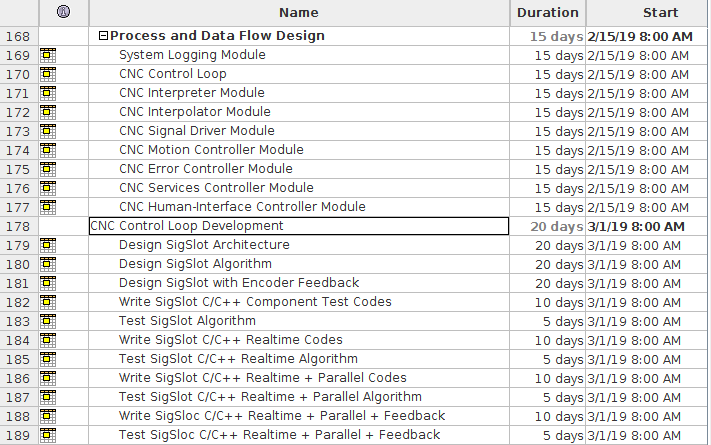
\includegraphics[width=1.00\textwidth]{./07-images/img-Ch5App/06-Research-Implementation-Plan.png}}
		\caption{App5-Process and Data Flow Design for the Control Loop}
		\label{fig:App5-06-Research-Implementation-Plan.png}
	\end{center}
\end{figure}

\pagebreak
\subsection{App5-Test-Case Based Design in Software Construction}
\begin{figure}[htbp]
	\begin{center}
		\frame{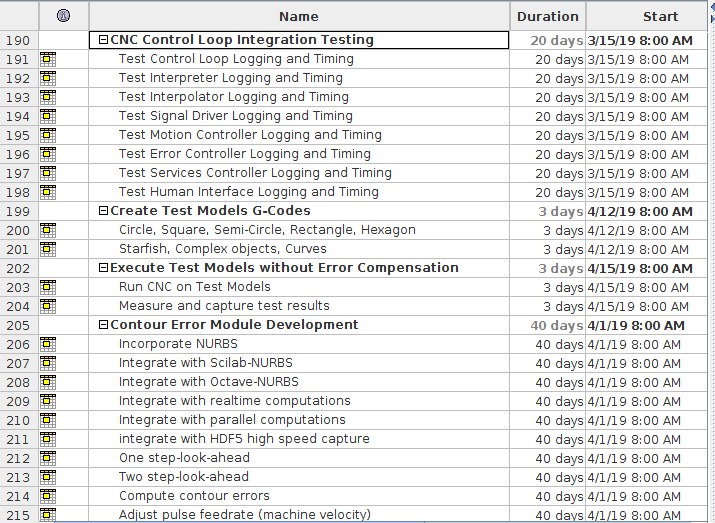
\includegraphics[width=1.00\textwidth]{./07-images/img-Ch5App/07-Research-Implementation-Plan.png}}
		\caption{App5-Test-Case Based Design in Software Construction}
		\label{fig:App5-07-Research-Implementation-Plan.png}
	\end{center}
\end{figure}

\pagebreak
\subsection{App5-Completion Testing, Publication Plan and Project Closing}
\begin{figure}[htbp]
	\begin{center}
		\frame{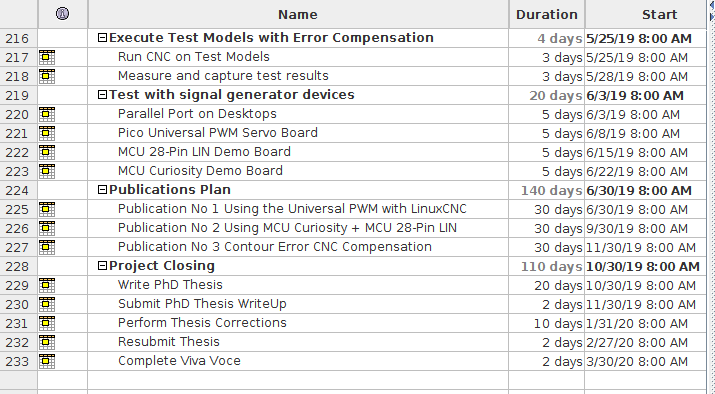
\includegraphics[width=1.00\textwidth]{./07-images/img-Ch5App/08-Research-Implementation-Plan.png}}
		\caption{App5-Completion Testing, Publication Plan and Project Closing}
		\label{fig:App5-08-Research-Implementation-Plan.png}
	\end{center}
\end{figure}

% ==========================================================
% ==========================================================
\clearpage
\begin{landscape}
\subsection{App5-Computer Notebook Specifications}
	
\begin{table}[ht]
\begin{center}
\caption{App5-Computer Notebook Specifications}		
\label{table:App5-Computer Notebook Specifications}	
	
\begin{tabular}{ |p{0.5cm}|p{5.0cm}|p{9.0cm}|p{9.0cm}|}
	\rowcolor{gray!10}			
	\hline \multicolumn{4}{|c|}{\textbf{Computer Notebook Specifications}} \\ [1.0ex]
	\rowcolor{gray!10}
	\hline \textbf{No} & \textbf{Specifications}    & \textbf{Hewlett Packard EliteBook 8470p} & \textbf{Hewlett Packard ProBook 440G}\\ 

	\hline 1 & Name of Student    & Wan Ruslan bin W Yusoff & hello\\ 
	\hline 2 & Student ID         &  aaa & Hello\\ 
	\hline 3 & National Reg. ID   & bbb  & Hello\\ 
	\hline 4 & Faculty            & ccc  & Hello\\ 

	\hline
\end{tabular}
\end{center}
\end{table}  
	
	
\end{landscape}
% ==========================================================
% ==========================================================
\clearpage
\begin{landscape}
\subsection{App5-Computer Desktop Specifications}
	
	\begin{table}[ht]
		\begin{center}
			\caption{App5-Computer Desktop Specifications}		
			\label{table:App5-Computer Desktop Specifications}	
			
			\begin{tabular}{ |p{0.5cm}|p{5.0cm}|p{9.0cm}|p{9.0cm}|}
				\rowcolor{gray!10}			
				\hline \multicolumn{4}{|c|}{\textbf{Computer Desktop Specifications}} \\ [1.0ex]
				\rowcolor{gray!10}
				\hline \textbf{No} & \textbf{Specifications}  & \textbf{WRY Intel Desktop} & \textbf{WRY SGI Desktop}\\ 
				
				\hline 1 & Name of Student    & Wan Ruslan bin W Yusoff & hello\\ 
				\hline 2 & Student ID         &  aaa & Hello\\ 
				\hline 3 & National Reg. ID   & bbb  & Hello\\ 
				\hline 4 & Faculty            & ccc  & Hello\\ 
				
				\hline
			\end{tabular}
		\end{center}
	\end{table}  
	
	
\end{landscape}
% ==========================================================
% ==========================================================
\clearpage
\begin{landscape}
\subsection{App5-Pulse Generator Interface Boards}
	
	\begin{table}[ht]
		\begin{center}
			\caption{App5-Pulse Generator Interface Boards}		
			\label{table:App5-Pulse Generator Interface Boards}	
			
			\begin{tabular}{ |p{0.5cm}|p{5.0cm}|p{6.0cm}|p{6.0cm}|p{6.0cm}|}
				\rowcolor{gray!10}			
				\hline \multicolumn{5}{|c|}{\textbf{Pulse Generator Interface Boards}} \\ [1.0ex]
				\rowcolor{gray!10}
				\hline \textbf{No} & \textbf{Specifications}    & \textbf{Pico Universal PWM Servo Controller Board} & \textbf{MCU Microchip 28-Pin LIN Development Board} & \textbf{MCU Microchip Curiosity Development Board}\\ 
				
				\hline 1 & Name of Student    & Wan Ruslan bin W Yusoff & hello & Hello\\ 
				\hline 2 & Student ID         &  aaa & Hello & hello\\ 
				\hline 3 & National Reg. ID   & bbb  & Hello & Hello \\ 
				\hline 4 & Faculty            & ccc  & Hello & Hello\\ 
				
				\hline
			\end{tabular}
		\end{center}
	\end{table}  
	
	
\end{landscape}
% ==========================================================
% ==========================================================
\clearpage
\begin{landscape}
\subsection{App5-Software Programming Language Features}

	
	\begin{table}[ht]
		\begin{center}
			\caption{App5-Software Programming Language Features}		
			\label{table:App5-Software Programming Language Features}	
			
			\begin{tabular}{ |p{0.5cm}|p{5.0cm}|p{9.0cm}|p{9.0cm}|}
				\rowcolor{gray!10}			
				\hline \multicolumn{4}{|c|}{\textbf{Software Programming Language Features}} \\ [1.0ex]
				\rowcolor{gray!10}
				\hline \textbf{No} & \textbf{Specifications}    & \textbf{Hewlett Packard EliteBook 8470p} & \textbf{Hewlett Packard ProBook 440G}\\ 
				
				\hline 1 & Name of Student    & Wan Ruslan bin W Yusoff & hello\\ 
				\hline 2 & Student ID         &  aaa & Hello\\ 
				\hline 3 & National Reg. ID   & bbb  & Hello\\ 
				\hline 4 & Faculty            & ccc  & Hello\\ 
				
				\hline
			\end{tabular}
		\end{center}
	\end{table}  
	
	
\end{landscape}
% ==========================================================
% ==========================================================
\clearpage
\begin{landscape}
\subsection{App5-Software Programming Paradigms}
	
	\begin{table}[ht]
		\begin{center}
			\caption{App5-Software Programming Paradigms}		
			\label{table:App5-Software Programming Paradigms}	
			
			\begin{tabular}{ |p{0.5cm}|p{5.0cm}|p{9.0cm}|p{9.0cm}|}
				\rowcolor{gray!10}			
				\hline \multicolumn{4}{|c|}{\textbf{Software Programming Paradigms}} \\ [1.0ex]
				\rowcolor{gray!10}
				\hline \textbf{No} & \textbf{Specifications}    & \textbf{Hewlett Packard EliteBook 8470p} & \textbf{Hewlett Packard ProBook 440G}\\ 
				
				\hline 1 & Name of Student    & Wan Ruslan bin W Yusoff & hello\\ 
				\hline 2 & Student ID         &  aaa & Hello\\ 
				\hline 3 & National Reg. ID   & bbb  & Hello\\ 
				\hline 4 & Faculty            & ccc  & Hello\\ 
				
				\hline
			\end{tabular}
		\end{center}
	\end{table}  
	
\end{landscape}	
% ==========================================================
% ==========================================================
\clearpage
\begin{landscape}
	\subsection{App5-Scilab NURBS versus Octave NURBS packages}
	
	\begin{table}[ht]
		\begin{center}
			\caption{App5-Scilab NURBS versus Octave NURBS packages}		
			\label{tabl2:App5-Scilab NURBS versus Octave NURBS packages}	
			
			\begin{tabular}{ |p{0.5cm}|p{5.0cm}|p{9.0cm}|p{9.0cm}|}
				\rowcolor{gray!10}			
				\hline \multicolumn{4}{|c|}{\textbf{Scilab NURBS versus Octave NURBS packages}} \\ [1.0ex]
				\rowcolor{gray!10}
				\hline \textbf{No} & \textbf{Specifications}    & \textbf{Hewlett Packard EliteBook 8470p} & \textbf{Hewlett Packard ProBook 440G}\\ 
				
				\hline 1 & Name of Student    & Wan Ruslan bin W Yusoff & hello\\ 
				\hline 2 & Student ID         &  aaa & Hello\\ 
				\hline 3 & National Reg. ID   & bbb  & Hello\\ 
				\hline 4 & Faculty            & ccc  & Hello\\ 
				
				\hline
			\end{tabular}
		\end{center}
	\end{table}  
	
\end{landscape}
% ==========================================================
% ==========================================================
\clearpage
\begin{landscape}
	\subsection{App5-Python versus Julia programming languages}
	
	\begin{table}[ht]
		\begin{center}
			\caption{App5-Python versus Julia programming languages}		
			\label{tabl2:App5-Python versus Julia programming languages}	
			
			\begin{tabular}{ |p{0.5cm}|p{5.0cm}|p{9.0cm}|p{9.0cm}|}
				\rowcolor{gray!10}			
				\hline \multicolumn{4}{|c|}{\textbf{Python versus Julia programming languages}} \\ [1.0ex]
				\rowcolor{gray!10}
				\hline \textbf{No} & \textbf{Specifications}    & \textbf{Hewlett Packard EliteBook 8470p} & \textbf{Hewlett Packard ProBook 440G}\\ 
				
				\hline 1 & Name of Student    & Wan Ruslan bin W Yusoff & hello\\ 
				\hline 2 & Student ID         &  aaa & Hello\\ 
				\hline 3 & National Reg. ID   & bbb  & Hello\\ 
				\hline 4 & Faculty            & ccc  & Hello\\ 
				
				\hline
			\end{tabular}
		\end{center}
	\end{table}  
	
\end{landscape}
% ==========================================================
% ==========================================================
\clearpage
\begin{landscape}
	\subsection{App5-C/C++ versus Rust system programming languages}
	
	\begin{table}[ht]
		\begin{center}
			\caption{App5-C/C++ versus Rust system programming languages}		
			\label{tabl2:App5-C/C++ versus Rust system programming languages}	
			
			\begin{tabular}{ |p{0.5cm}|p{5.0cm}|p{9.0cm}|p{9.0cm}|}
				\rowcolor{gray!10}			
				\hline \multicolumn{4}{|c|}{\textbf{C/C++ versus Rust system programming languages}} \\ [1.0ex]
				\rowcolor{gray!10}
				\hline \textbf{No} & \textbf{Specifications}    & \textbf{Hewlett Packard EliteBook 8470p} & \textbf{Hewlett Packard ProBook 440G}\\ 
				
				\hline 1 & Name of Student    & Wan Ruslan bin W Yusoff & hello\\ 
				\hline 2 & Student ID         &  aaa & Hello\\ 
				\hline 3 & National Reg. ID   & bbb  & Hello\\ 
				\hline 4 & Faculty            & ccc  & Hello\\ 
				
				\hline
			\end{tabular}
		\end{center}
	\end{table}  
	
\end{landscape}
% ==========================================================
% ==========================================================
 %% Research Implementation Plan
	%\input{Appendix-Chap-6} %% Conclusion ==> NOT APPLICABLE
	\input{Chapter-10-Index}  %% ADDED TEMPORARILY
	...
	...
\end{lstlisting}
\end{tcolorbox}

%	\pagebreak
%% ===========================================
\begin{tcolorbox}

\section{zzAdvice-on-Indexing}





\textbf{INDEXING HOW TO Guidelines - TO REMOVE LATER}	
% \vspace*{1\baselineskip}

% ==========================================================
\lstset{basicstyle=\footnotesize, numberstyle=\tiny\color{blue}, frame=single, numbers=left, firstnumber=1, stepnumber=1, numbersep=1pt, xleftmargin=2.0em, framexleftmargin=1.5em, xrightmargin=0.0em, breaklines=true, breakatwhitespace=false, breakindent=5pt, prebreak=\space, postbreak=\space }
% ==========================================================
\begin{lstlisting}[caption={zzAdvice-on-Indexing}, label=zzAdvice-on-Indexing]

% (1) INFO FOR APPENDICES

Since glossaries-extra internally loads the glossaries package, you also need to have glossaries installed and all the packages that glossaries depends on (including, but not limited to, tracklang, mfirstuc, etoolbox, xkeyval (at least version dated 2006/11/18), textcase, xfor, datatool-base and amsgen

REF: glossaries-extra Manual
This glossary style was setup using:

\usepackage[xindy,
	nonumberlist,
	toc,
	nopostdot,
	style=altlist,
	nogroupskip]{glossaries}

bib2gls = An indexing application that combines two functions in one: 

	(1) fetches entry definition from a .bib file based on information provided in the .aux file (similar to bibtex); 
	
	(2) hierarchically sorts and collates location lists (similar to makeindex and xindy). This application is designed for use with glossaries-extra and can not be used with just the base glossaries package.



% (2) PLACED INSIDE PREAMBLE SECTION


% (3) PLACED INSIDE DOCUMENT SECTION


% (4) EXAMPLES

	\section{Index - TO DO}
	
	idx = index file\\
	ist = file\\
	acr = file\\
	acn = acronym file\\
	gls = glossary file\\
	glo = glossary file\\
	Command line shell script (/bin/bash). \\
	
	%% #!/bin/bash\\
	makeindex MainRoot-doc.idx\\
	makeindex -s MainRoot-doc.ist -o MainRoot-doc.acr MainRoot-doc.acn\\
	makeindex -s MainRoot-doc.ist -o MainRoot-doc.gls MainRoot-doc.glo\\
	pdflatex MainRoot-doc.tex\\
	pdflatex MainRoot-doc.tex\\
	%% echo "Alhamdulillah 3 times WRY. \n"

...
...
\end{lstlisting}
\end{tcolorbox}


\pagebreak

%% ===========================================

\section{zzAdvice-on-Using-Links}

\textbf{HOW-TO Develop different Links in latex document - TO REMOVE LATER}	
\vspace*{1\baselineskip}
	
\textbf{ACTUAL OUTPUT DISPLAY IN PDF DOCUMENT}
\vspace*{1\baselineskip}	

\begin{tcolorbox}	
% ==========================================================
TESTING 1 (NOT VISIBLE FOR Index ITEMS IN MAIN DOCUMENT)
% ==========================================================
\vspace*{1\baselineskip}

\begin{enumerate}
	
	\item \index{Interpolation}  				 IS NOT VISIBLE
	\item \index{Digital Differential Analyser}  IS NOT VISIBLE
	
\end{enumerate}
\vspace*{1\baselineskip}

% ==========================================================	
TESTING 2 (VISIBLE FOR Citation, Glossary, Acronym, Website LINKS)
% ==========================================================
\vspace*{1\baselineskip}

ALL VISIBLE ITEMS WILL BE COLORED BLUE (AS HYPERLINKS IN PDF.
\vspace*{1\baselineskip}

\begin{enumerate}
	
	\item Ref\cite{FYP_Abzal_2012} internal link to Reference-List(tex) (Bibliography)
	
	\item Acrn[\gls{cnc}] internal link to Acronym-List (tex)
	
	\item Gloss[\gls{cnc-control-loop}] internal link to Glossary-List (tex)
	
	\item Figure[\ref{fig:CNC-Research-Machine-3-Axis.jpg}] internal link to Figures 
	
	\item Table[\ref{table:CNC-Terminology Part 1 of 2}] internal link to Tables
	
	\item Listing[\ref{App4-Full execution C/C++ code for Real Time (RTAI)}] internal link to Listings 
	
	\item Website: \href{https://www.linux.org/}{LINUX.ORG} external link to the internet (URL)
	
\end{enumerate}


\end{tcolorbox}

\clearpage
\pagebreak
	
\textbf{LATEX CODE BEHIND THE SCENE FOR PREVIOUS PAGE}
\vspace*{1\baselineskip}

% ==========================================================
\lstset{basicstyle=\footnotesize, numberstyle=\tiny\color{blue}, frame=single, numbers=left, firstnumber=1, stepnumber=1, numbersep=1pt, xleftmargin=2.0em, framexleftmargin=1.5em, xrightmargin=0.0em, breaklines=true, breakatwhitespace=false, breakindent=5pt, prebreak=\space, postbreak=\space }
% ==========================================================

\begin{lstlisting}[caption={Advice on Latex codes for making links}, label=lst:Advice on Latex codes for making links]

% ==========================================================
TESTING 1 (NOT VISIBLE FOR Index ITEMS IN MAIN DOCUMENT)
% ==========================================================

\begin{enumerate}

	\item \index{Interpolation}			IS NOT VISIBLE
	\item \index{Digital Differential Analyser}	IS NOT VISIBLE
	
\end{enumerate}

% ==========================================================	
TESTING 2 (VISIBLE FOR Citation, Glossary, Acronym & Website LINKS)
% ==========================================================

	ALL VISIBLE ITEMS WILL BE COLORED BLUE (AS HYPERLINKS IN PDF.

\begin{enumerate}
		
	\item Ref\cite{FYP_Abzal_2012} internal link to Reference-List(tex) (Bibliography)
	
	\item Acrn[\gls{cnc}] internal link to Acronym-List (tex)
	
	\item Gloss[\gls{cnc-control-loop}] internal link to Glossary-List (tex)
	
	\item Figure[\ref{fig:CNC-Research-Machine-3-Axis.jpg}] internal link to Figures 

	\item Table[\ref{table:CNC-Terminology Part 1 of 2}] internal link to Tables

	\item Listing[\ref{App4-Full execution C/C++ code for Real Time (RTAI)}] internal link to Listings 
	
	\item Website: \href{https://www.linux.org/}{LINUX.ORG} external link to the internet (URL)

\end{enumerate}

%% =====================================

Reading raw-index "/tmp/tpMuNrBM7K"...
Finished reading raw-index.

Processing index... [10%] [20%] [30%] [40%] [50%] [60%] [70%] [80%] [90%] [100%]
Finished processing index.

Writing markup... [10%] [20%] [30%] [40%] [50%] [60%] [70%] [80%] [90%] [100%]
Markup written into file "./Draft-39-PhD-Proposal-WRY.ind".

\end{lstlisting}	
% =============================================	

\clearpage
\pagebreak

\textbf{LATEX CODE BEHIND THE SCENE FOR PREVIOUS PAGE}
\vspace*{1\baselineskip}

% ==========================================================
\lstset{basicstyle=\footnotesize, numberstyle=\tiny\color{blue}, frame=single, numbers=left, firstnumber=1, stepnumber=1, numbersep=1pt, xleftmargin=2.0em, framexleftmargin=1.5em, xrightmargin=0.0em, breaklines=true, breakatwhitespace=false, breakindent=5pt, prebreak=\space, postbreak=\space }
% ==========================================================

\begin{lstlisting}[caption={Advice on Latex codes behind the scene}, label=lst:Advice on Latex codes behind the scene]


wruslan@HPProBk440G-ub1604-rtai-64b:~/Downloads/Draft-39-Report-Latex-Proposal-Writeup$ cat ./run-makeglossaries-texindy.sh 
#!/bin/bash
echo "Bismillah WRY. Execute run-makeglossaries-texindy.sh \n"
echo

makeglossaries Draft-39-PhD-Proposal-WRY.tex
pdflatex       Draft-39-PhD-Proposal-WRY.tex

makeindex      Draft-39-PhD-Proposal-WRY.idx

makeindex -s   Draft-39-PhD-Proposal-WRY.ist -t Draft-39-PhD-Proposal-WRY.glg -o Draft-39-PhD-Proposal-WRY.gls Draft-39-PhD-Proposal-WRY.glo

makeindex -s   Draft-39-PhD-Proposal-WRY.ist -t Draft-39-PhD-Proposal-WRY.glg -o Draft-39-PhD-Proposal-WRY.acr Draft-39PhD-Proposal-WRY.acn

makeindex -s   Draft-39-PhD-Proposal-WRY.ist -t Draft-39-PhD-Proposal-WRY.glg -o Draft-39-PhD-Proposal-WRY.gls Draft-39-PhD-Proposal-WRY.glo

makeindex -s   Draft-39-PhD-Proposal-WRY.ist -t Draft-39-PhD-Proposal-WRY.glg -o Draft-39-PhD-Proposal-WRY.nls Draft-39-PhD-Proposal-WRY.nlo

texindy		   Draft-39-PhD-Proposal-WRY.tex
pdflatex       Draft-39-PhD-Proposal-WRY.tex
pdflatex       Draft-39-PhD-Proposal-WRY.tex


echo
echo "SUCCESS. Alhamdulillah 3 times WRY."
echowruslan@HPProBk440G-ub1604-rtai-64b:~/Downloads/Draft-39-Report-Latex-Proposal-Writeup$ 

\end{lstlisting}	
% =============================================	



\justifying
\noindent

\titleformat{\chapter}{\normalfont\huge\bfseries\color{black}}{\thechapter}{10pt}{\huge} 
\chapter{Introduction}

%% \input{Advice-for-Chapter-1}
\justifying
\noindent

\section{Introduction}

With the availability of increased processing power and memory of personal computers, today Computer Numerical Control (CNC) interpolation is mostly carried out using computer software instead of electronic hardware devices with mathematical logic, for example, the Digital Differential Analyser (DDA) integrator. The basic theory and design of CNC systems, however, have remain the same since its beginning \cite{SuhBook_2008}. 
\vspace*{1\baselineskip}


The two common types of CNC software interpolation techniques are Reference-Pulse Interpolation \cite{Giap_2014},\cite{Koren_1981}, and Reference-Word (Sampled-Data) Interpolation \cite{Koren_1982}, \cite{Koren_1978}. 

	%% NOT VISIBLE
	\index{Reference-Pulse interpolation}
	\index{Reference-Word interpolation} 
	\index{Sampled-Data interpolation}
	\vspace*{1\baselineskip}

Over time, various algorithms have been proposed for CNC software interpolation. For example, techniques for Reference-Pulse interpolation include software version of the Digital Differential Analyser (SDDA), the Stairs Approximation and the Direct Search Interpolation. 

	%% NOT VISIBLE
	\index{Digital Differential Analyser} 
	\index{Stairs Approximation interpolation} 
	\index{Direct Search interpolation}
	\vspace*{1\baselineskip}

Techniques for Reference-Word interpolation include Euler, Improved Euler, Taylor, Tustin and Improved Tustin interpolations.

	%% NOT VISIBLE
	\index{Euler interpolation}
	\index{Improved Euler interpolation}
	\index{Taylor interpolation}
	\index{Tustin interpolation}
	\index{Improved Tustin interpolation}
	\vspace*{1\baselineskip}

In CNC machine operation, the function of interpolation is to generate coordinated movements to drive the separate axis-of-motions and/or rotation axes in order to achieve the desired path of the CNC cutting or milling tool relative to the workpiece. Essentially, interpolation generates the final reference commands that moves stepper or servo motor drives to produce the physical part that is to be machined. Reference commands mean commands to the CNC tool to trace/follow (refer to) the desired path or trajectory.

%% NOT VISIBLE
	\index{Milling tool}
	\index{Reference command}

% =====================================
\section{Types of CNC Machines}
%======================================

There are various types of CNC machines. The main categories are CNC Milling, CNC Lathe, CNC Router and CNC 3D Printing machines. There are many sub-categories, covering variations of CNC machines, and it is too numerous to list. 
\vspace*{1\baselineskip}

These machines share one common characteristic, that is, they all are numerically controlled by a computer, thus adopting the name Computer Numerical Control (CNC) machines. Most CNC machines cut or remove materials in order to produce a machined part. The exception is the CNC 3D Printing machine where materials are instead deposited layer by layer to produce a part.

\subsection{CNC Milling Machine}

CNC milling devices are the most widely used type of CNC machine. It is a machine that produces a work part by both drilling and cutting using a rotating cylindrical cutting tool. In a milling machine, the cutter is able to move along multiple axes simultaneously. It can create a part with a variety of shapes, slots and holes. To produce a part, the work-piece in a milling machine is often moved across the milling tool (drill cutter) in different directions, like linear table movements and circular table rotations.  Common milling machines offer from 3 to 5 motion axes. Please see Fig. ~\ref{fig:App1-CNC-Milling-Machine.jpg}, a link to the image of a typical CNC Milling machine.

\subsection{CNC Lathe Machine}

The CNC lathe machine is a machine that rotates a workpiece on a spindle to cut away excess material. The lathe uses cutting tools and drill bits with different diameters to apply on the workpiece and produce a symmetrical object. In a lathe machine, the cutter is not able to move along multiple axes. These machines can produce objects in a variety of shapes, cuts, and details based on cutting a rotating work piece. The two lathe configuration types are the CNC horizontal lathe and the CNC vertical lathe. Please see Fig. ~\ref{fig:App1-CNC-Lathe-Machine.jpg}, a link to the image of a typical CNC Lathe machine.

\subsection{CNC Router Machine}

The CNC router machine is very similar in concept to a CNC milling machine. Instead of routing by hand, tool paths for the CNC router are controlled via computer numerical control system. The word rout means to "hollow out" an area in relatively hard material. Routers are normally used for cutting various hard materials, such as engraving wood, composites, aluminum, steel, ceramics, plastics, glass, and foams. The application of routers are mainly in woodworking, especially building cabinets,  engraving decorations, doors or panels. Routers are not generally used for drilling or 3D model machining. Please see Fig. ~\ref{fig:App1-CNC-Routing-Machine.jpg}, a link to the image of a typical CNC Routing machine.

\subsection{CNC 3D Printing}

The CNC 3D Printing machine is a machine in which material is deposited, joined or solidified under computer control to create a three-dimensional object. Many different technologies are used in the 3D printing process, the most common being the fused deposit modeling (FDM) method. The machine uses inkjet-technology nozzles to apply a specialized thick liquid or powder to form each new layer. Common materials used in 3D printing are thick waxes and plastic polymers. 
Please see Fig. ~\ref{fig:App1-CNC-3D-Printing-Machine.jpg}, a link to the image of a typical CNC 3D Printing machine.

%% =================================
\subsection{Recent Designs in CNC Systems}

On designs in CNC machine architectures, recent developments in CNC systems include, for example, designs with the introduction of more motion axes (up to 9 axes), cutting under water or fluid immersion environments, new sensors, smart computing, high-speed machining, energy efficient techniques, artificial intelligence control, wastage reduction in materials removal, process monitoring, machining management operations, modular software construction, and human-machine interface. 
\vspace*{1\baselineskip}

On designs in CNC machining control, new developments include design, for example, in software algorithms and methods, for path motion smoothness, for machining speed control, for addressing acceleration and deceleration effects, for 2D path error reduction, for 3D contouring error control, for compensating tool jerks, vibrations, heating and friction effects.         


\pagebreak
\clearpage
% ==========================================
\section{Basic architecture of a typical CNC system} 

\begin{figure}[htbp]
	\begin{center}
		\frame{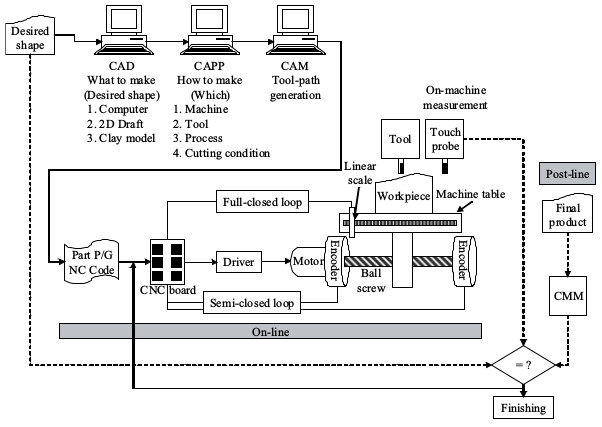
\includegraphics[width=0.95\textwidth]{./07-images/img-Ch1/CNC-Basic-Architecture.jpg}}
		\caption{Basic architecture of a typical CNC system.}
		\label{fig:CNC-Basic-Architecture.jpg}
	\end{center}
\end{figure}

\begin{figure}[htbp]
	\begin{center}
		\frame{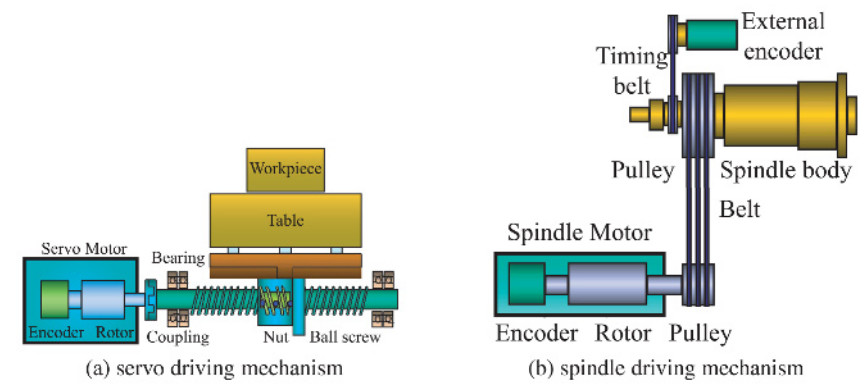
\includegraphics[width=0.68\textwidth]{./07-images/img-Ch1/CNC-Servo-and-Spindle-Driving-Mechanism.jpg}}
		\caption{CNC Servo and Spindle Driving Mechanism}
		\label{fig:CNC-Servo-and-Spindle-Driving-Mechanism.jpg}
	\end{center}
\end{figure}


\pagebreak
\clearpage
% ==========================================
\section{Process Flow for a typical CNC system}

\begin{figure}[htbp]
	\begin{center}
		\frame{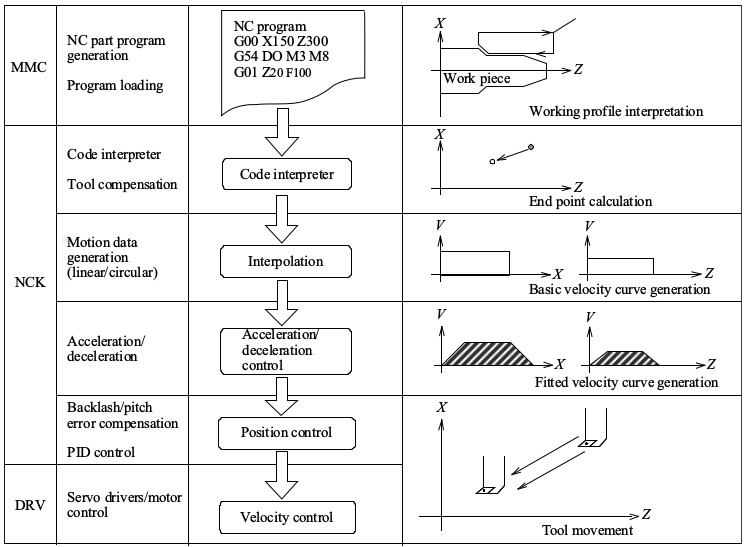
\includegraphics[width=0.98\textwidth]{./07-images/img-Ch1/CNC-Typical-Software-Control-Flow-Diagram.jpg}}
		\caption{Process Flow for a typical CNC system}
		\label{fig:CNC-Typical-Software-Control-Flow-Diagram.jpg}
	\end{center}
\end{figure}

Legend\\
\begin{enumerate}
	\item MMC Man-Machine Control
	\item NCK Numerical Control Kernel
	\item DRV Driver Module
	\item NC  Numerical Control
	\item PID Proportional Integrative Derivative
\end{enumerate}


\pagebreak
\clearpage
% ==========================================
\section{Functional block diagram for a typical CNC system} 

CNC manufacturing operations involve the generation of reference signals describing the geometrical parts to be machined and the control of the machine. The control is such that it follows those reference signals. In modern CNC machines, the generation of reference signals, construction and execution of control loops are accomplished in software within a computer.    
\vspace*{1\baselineskip}

The figure below shows the functional block diagram for a typical CNC system. The meanings of terms used are described in Table [~\ref{table:CNC-Terminology Part 1 of 2}] and Table [~\ref{table:CNC-Terminology Part 2 of 2}]. 

\begin{figure}[htbp]
	\begin{center}
		\frame{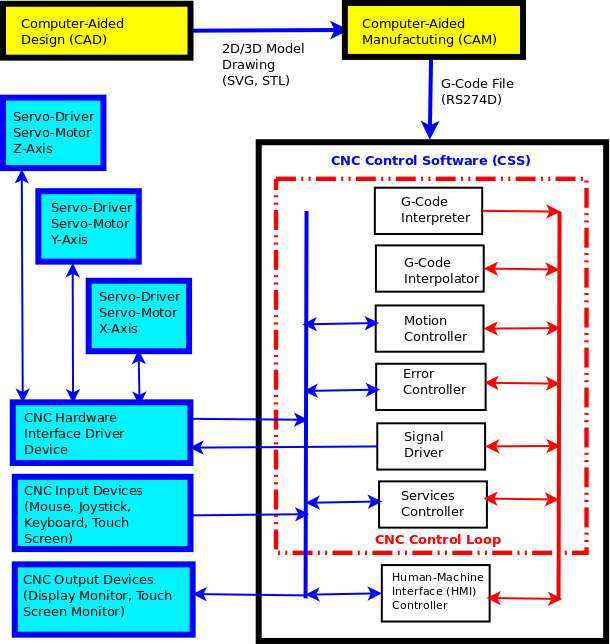
\includegraphics[width=0.95\textwidth]{./06-diagrams/dia-Ch1/Components-of-CNC-System.jpg}}
		\caption{Functional Block Diagram for CNC system}
		\label{fig:Functional-Block-Diagram-for-CNC-System.jpg}
	\end{center}
\end{figure}

% =========================================
%%\clearpage
%%\pagebreak

%% \section{Process flow chart for a typical CNC system}

%% YES. tikz package working
%%% =========================================================
% % \input{./diagrams/dia-Ch1/test-tikz.tex}
% =========================================================

%% TikZ is a very large program which can do lots of things. You will find commands to draw hierarchial trees, to draw lots of different types of shapes, to do some elementary programming, to align elements of a picture in a matrix frame, to decorate nodes, to compute the intersections of paths, etc.  The main message is “if it is not in these notes, it is most probably somewhere in the manual”


\begin{center}
\begin{tikzpicture}

\draw [<->] (0,2) -- (0,0) -- (4,0);
\draw [thick] (0,1.5) -- (3,0);
\draw [ultra thick] (0,0) -- (2,2);
\draw [help lines] (1,0) -- (1,1) -- (0,1);

\draw [blue] (0,0) rectangle (1.5,1);
\draw [red, ultra thick] (3,0.5) circle [radius=0.5];;
\draw [gray] (6,0) arc [radius=1, start angle=45, end angle= 120];


\draw [<->, rounded corners, ultra thick, purple] (0,2) -- (0,0) -- (3,0) -- (10, 10);


\draw [gray, ultra thick] (6,8) arc [radius=5, start angle=45, end angle= 65];

\draw[very thick] (0,0) to [out=90,in=195] (10,10);

\draw [<->, help lines] (0.6,1.34) -- (0.6,1) -- (1.05,1);
\draw[blue, ultra thick] (0.6, 1.0385) -- (0.61, 1.06372) -- (0.62, 1.08756) -- (0.63, 1.11012) -- (0.64,1.13147) -- (0.65, 1.15166) -- (0.66, 1.17074) -- (0.67, 1.18874) -- (0.68,1.20568) -- (0.69, 1.22157) -- (0.7, 1.23643) -- (0.71, 1.25026) -- (0.72,1.26307) -- (0.73, 1.27486) -- (0.74, 1.28561) -- (0.75, 1.29534) -- (0.76, 1.30402) -- (0.77, 1.31165) -- (0.78, 1.31821) -- (0.79, 1.32369) -- (0.8, 1.32806) -- (0.81, 1.33131) -- (0.82, 1.3334) -- (0.83, 1.33431) -- (0.84, 1.334) -- (0.85, 1.33244) -- (0.86, 1.32956) -- (0.87, 1.32533) -- (0.88, 1.31966) -- (0.89, 1.3125) -- (0.9, 1.30373) -- (0.91, 1.29325) -- (0.92, 1.2809) -- (0.93, 1.26649) -- (0.94, 1.24976) -- (0.95, 1.23032) -- (0.96, 1.2076) -- (0.97, 1.18065) -- (0.98, 1.14763) -- (0.99, 1.1038) -- (0.991, 1.09836) -- (0.992, 1.09261) -- (0.993, 1.0865) -- (0.994, 1.07994) -- (0.995, 1.07282) -- (0.996, 1.06497) -- (0.997, 1.0561) -- (0.998, 1.04563) -- (0.999, 1.03209) -- (0.9991, 1.03042) -- (0.9992, 1.02866) -- (0.9993, 1.02679) -- (0.9994, 1.02478) -- (0.9995, 1.0226) -- (0.9996, 1.02019) -- (0.9997, 1.01747) -- (0.9998, 1.01424) -- (0.9999, 1.01005) -- (0.9999, 1.01005) -- (0.99991, 1.00953) -- (0.99992, 1.00898) -- (0.99993, 1.0084) -- (0.99994, 1.00778) -- (0.99995, 1.0071) -- (0.99996, 1.00634) -- (0.99997, 1.00549) -- (0.99998, 1.00448) -- (0.99999, 1.00317) -- (1,1);
\end{tikzpicture}
\end{center}


\begin{center}
\begin{tikzpicture}[domain=0:0.5,xscale=10,yscale=10]

\draw[<->] (0,2) node[left]{EUR}-- (0,0) -- (.7,0) node[below] {$q$};
\draw[red] plot (\x, {0.25+\x/2+\x*\x/2}) node[right] {$v_1(x)$};
\draw[green] plot (\x, {0.025+\x+\x*\x}) node[right] {$v_2(x)$};
\draw[thin, dashed] plot (\x, {0.275+1.5*\x+1.5*\x*\x}) ;
\draw[thick,domain=0:0.33666] plot (\x, {0.05+2*\x+2*\x*\x}) ;
\draw[thick,domain=0.33666:0.5]
plot (\x, {0.5+\x+\x*\x}) node[right] {$2\min[v_1,v_2]$};


\end{tikzpicture}
\end{center}

%% http://www.texample.net/

%% CREATE THE CNC OVERALL FLOW CHART
%\input{./diagrams/dia-Ch1/Flow-Chart-for-CNC-System.tex}


\clearpage
\pagebreak
% ==========================================
\subsection{CNC operations in CAD/CAM/CNC systems}

The overall CNC operations in parts manufacturing using CAD/CAM/CNC systems can be described as follows. 
\vspace*{1\baselineskip}

First, the part geometry to be machined is generated by a Computer Aided Design (CAD) system that produces a 2D or 3D geometrical or model drawing. 
\vspace*{1\baselineskip}

Next, the Computer Aided Manufacturing (CAM) system converts this geometrical drawing into a part program called its G-Code. This G-Code file consists of a list of motion and machine service commands that provide specific step-by-step instructions for the CNC machine to manufacture the part. The G-Code part program generated by the CAM system is governed by international standards. This standardization ensures that different CAD drawings can be converted to a standardized G-Code by different CAM systems. Thus, different CNC manufacturers can machine the common G-Code and produce identical machine parts.
\vspace*{1\baselineskip}
	
Next, a CNC interpreter program sequentially reads and interprets this G-Code commands, identifying whether the instruction is about tool movement processing, tool feedrate processing or machine function. For example, the prefix G in the part program instruction (G-Code) is for tool movement like a linear move or a circular arc move. This instruction moves the tool along the translational axes or along the rotary axes for some specified geometric path. The prefix M instruction is for controlling machine service functions like the start and stop of the tool cutting spindle. The prefix F instruction is for setting feedrates or speeds of tool movements along the translational axes or the rotary axes. 
\vspace*{1\baselineskip}

The next activity after CNC G-Code interpretation is CNC interpolation processing. CNC software interpolations cover linear, parametric and curve path contour commands provided in the G-Codes. The task of CNC G-Code interpolation is to process the interpreted G-Code and generate the final reference commands (referring to electrical signals) that drive the CNC tool along a pre-determined machining path. This contour path is normally constructed from a combination of linear and circular path segments. For example, interpolation generates reference commands that drive stepper or servo motors such that the required rotary or translational motions occur in a coordinated manner along the different axes simultaneously in tracing the desired contour path. In the process of CNC interpolation, the CNC Error Controller and CNC Motion Controller programs are executed based on to specific computation algorithms to achieve tracing accuracy along the desired contour path. These error-corrected or error-compensated outputs become machine reference commands (referring to the path) that drive the CNC motors. 
\vspace*{1\baselineskip}

The machine reference commands basically form a list of software machine instructions, saved in a CNC Signal File. The machine instructions in the signal file are read by the CNC Signal Driver in the CNC control loop and then transmitted to the CNC Hardware Interface Driver, which in turn, converts the software machine instructions that finally generates electrical pulses that drive the CNC electric motors. 

\begin{tcolorbox}[colback=green!15!white,colframe=red!75!black,title=Research consideration no. 1]	
The machine part to be manufactured is considered finished when the execution of the full list of reference commands completes and the CNC control loop exits.
\end{tcolorbox}

\pagebreak
\subsection{Interpreter and interpolator}
% ================================

The interpreter and the interpolator programs are specific to a particular CNC machine. The programs are different across different CNC machines due to differences, for example, in machine hardware configurations, in number of motion axes, in functions of cutting tools, in machine service functions, in G-Code standards adoption, and so on. It is therefore, standard practice that most hardware manufacturers create their own proprietary interpreter and interpolator programs for their CNC machines. These program codes are not public.

\begin{tcolorbox}[colback=green!15!white,colframe=red!75!black,title=Research consideration no. 1]
\justifying	
Based on the above reason, in this research project, the development of our own interpreter and interpolator programs is our primary goal.
\end{tcolorbox}

\subsection{Interpolation Task}
% ================================

In CNC interpolation, it is important to differentiate between CAM model interpolation and CNC G-Code interpolation to avoid confusion. The CAM interpolation process converts 2D/3D model drawings to produce G-Codes files, whereas the CNC interpolation process converts G-Codes files into electrical signals to drive CNC motors. 
\vspace*{1\baselineskip}

Most advanced CAM software are commercial, not cost-free like many open-source type software. They are written by experts with well grounded knowledge in the mathematics of geometrical model representations for 2D and 3D objects. We do not want to be CAM designers, thus we leave CAM model interpolation to the experts. 

\begin{tcolorbox}[colback=green!15!white, colframe=red!75!black, title=Research consideration no. 2]
\justifying
For the above reasons, in this research project, CNC G-Code software interpolation is our only concern. CAM interpolation is not in our scope.
\end{tcolorbox}

\subsection{Starting point of CNC operations}
% =====================================

Even though the CAD/CAM portion is not considered a component part of the CNC system, it plays an important initial role in the generation of G-Codes files. A high end and full-featured CAD/CAM system can produce G-Codes of different quality and contain different depths of manufacturing information. These sophisticated CAD/CAM applications can sometimes generate G-Codes complying to different G-Code standards.

\begin{tcolorbox}[colback=green!15!white, colframe=red!75!black, title=Research consideration no. 4]
\justifying
In this research project, we consider the start of CNC machine operation as beginning from G-Code processing stage, and not from the CAD/CAM stages. In addition, we will only use G-Code files conforming to the RS274-D NGC standard. Other G-Code standards are not in our scope. We will discuss this further in the section on literature review.
\end{tcolorbox}

\subsection{Online versus Offline processing}
% ===================================

In general, CNC Interpretation and CNC Interpolation can be conducted as online tasks, as offline tasks, or as a combination of both. In online mode, both interpretation and interpolation tasks are computed in memory and then fed into the CNC control loop while the loop is running. In offline mode, the interpretation and interpolation are pre-computed, stored in a file or memory and later fed to the CNC control loop. 
\vspace*{1\baselineskip}

The term realtime processing used synonymously to mean online processing in common CNC literature, is not technically correct. In software engineering, the terms are conceptually unrelated. We clarify this in the next section. 

\begin{tcolorbox}[colback=green!15!white, colframe=red!75!black, title=Research consideration no. 3]
\justifying
In this research project, we will implement and compare performances of both online and offline options. 
\end{tcolorbox}


\subsection{Realtime processing}
% =======================================

In general usage, people used the word "realtime" as processing at the current time instance. The layman use of the term realtime in communications is very different from its technical use in software. We illustrate the difference as follows: 
\vspace*{1\baselineskip}

In software terms, the definition of realtime processing is the execution of a process that meets its time deadline. There are strictly two(2) time deadlines for any event: the start deadline and the end deadline. 
\vspace*{1\baselineskip}

As an example, consider two event deadlines for the safety airbag in an car. The event deadline to start opening the airbag is \textbf{after} 0.20 seconds from time of impact, and the event deadline for reaching a fully blown airbag is \textbf{before} 0.50 seconds from time of impact. It means \textbf{both events} must occur within the specific duration. 
\vspace*{1\baselineskip}

The two events are considered realtime events if they both strictly meet their deadlines. This is the technical criteria for being realtime. Opening the air bag before 0.20 seconds (too early) means missing the deadline. Also reaching a full blown air bag after 0.50 seconds (too late) also means missing its deadline. In both cases, the car driver may already be dead. 
\vspace*{1\baselineskip}

In this case, the safety airbag is designed such that it must open only after 0.20 seconds of impact and must get to full blown state before 0.50 seconds from time of impact.  
\vspace*{1\baselineskip}

If the airbag reaches a partially blown state at 0.50 seconds, the effectiveness of the safety airbag may be compromised, meaning, the design cannot guarantee the full protection of the car driver. 
\vspace*{1\baselineskip}

In any field of engineering design (including software programming), there is no such thing as an event to occur precisely at an exact point in time. This is unrealistic because there is no such thing as instantaneous in electronic or mechanical systems. Any event can only occur within some time duration, no matter how short the duration (for example, in microsecond or nanosecond range). It could be somewhere in the nanosecond range for timing control of ballistic missiles, whereas it is typically in the order of milliseconds, even for the most advanced CNC systems. Realtime compliance is very important in high performance time processing. Finally we state the technical definition: A realtime event must precisely occur within its specified duration, that is between its start and end deadlines. 

\begin{tcolorbox}[colback=green!15!white, colframe=red!75!black, title=Research consideration no. 5]
\justifying
In this research project, realtime shall mean the software event or process must comply to the technical definition of realtime above. This will be achieved only when program codes are written using realtime capable programming languages, and the codes are executed on Real Time Operating System (RTOS) platforms. For correct performance, CNC processing events typically runs in the order of 10 milliseconds. We will discuss this further in the section on literature review.
\end{tcolorbox} 

% ===========================================
\subsection{Parallel processing}
% =======================================

Similarly, people have used the word "concurrent" as being synonymous with "parallel in time". In software terminology, we have to differentiate the layman use of the word parallel from its actual technical usage. We illustrate the difference between concurrent and parallel processes in software as follows: 
\vspace*{1\baselineskip}

Consider an example of a process where a person takes a jog and the jogging process is considered finished when the jogger reaches a specific destination. The jogger starts running and then along the way the jogger stops momentarily, to properly tie his loose shoe laces which took a few moments. During this short duration of tying the shoe lace, we consider the process of "shoe tying" and the process of "jogging" together as occurring concurrently. 
\vspace*{1\baselineskip}

Even though there is only a pause in the actual jogging, the jogging process is still considered ongoing because the destination has not yet being reached. When tightening the shoe laces in finished, the jogger resumes running until he reaches the destination, and then only the jogging process is considered finished. This is about concurrency. 
\vspace*{1\baselineskip}

All General Purpose Operating Systems (GPOS) platforms run their background processes concurrently. GPOS platforms are considered multi-tasking and time-sharing systems. Note that running in realtime (within start and end timing deadlines) and running in parallel are two separate concepts. 
\vspace*{1\baselineskip}

Next we explain about parallel processing. When two running processes or threads are executed on two separate CPUs independently at the same time, we say that the processes are truly running in parallel, meaning, overlapping in time. This is opposite to a sequential execution where one process must finish before another process can start. In parallel execution, processes truly run simultaneously or parallel in time.   

\begin{tcolorbox}[colback=green!15!white, colframe=red!75!black, title=Research consideration no. 6]
\justifying
In this research project, parallel shall mean simultaneously or overlapping in time. We shall implement program codes that run both in realtime and in parallel. We have successfully executed this before. We will discuss this further in the section on literature review.
\end{tcolorbox} 

\pagebreak
%% =======================================
\subsection{Recent interpolation Methods}
% =======================================

Recent techniques for CNC interpolation methods include advanced functions like look-ahead function, feedrate filtering  and Non-Uniform Rational B-Splines (NURBS) interpolation. We will describe them in the chapter on literature review.

\begin{tcolorbox}[colback=green!15!white, colframe=red!75!black, title=Research consideration no. 7]
For this research project, we will study different interpolation methods. We propose the look-ahead control and feedrate compensation methods for realtime and parallel CNC interpolation.
\end{tcolorbox}


% =========================================
\clearpage
\pagebreak
%% =========================================
%% File: inc: Table-Terminology-1of2.tex 
%% =========================================

\begin{table}[ht]
	\begin{center}
		\begin{tabular}{ |p{0.5cm}|p{3.4cm}|p{11.0cm}| }
			\rowcolor{LIGHTCYAN}			
			\hline \multicolumn{3}{|c|}{\textbf{CNC Terminology Part 1 of 2}} \\ [1.0ex]
			
			\hline 1,2  & S/W	and H/W	      & Software and Hardware\\ 
	
			\hline 3 & CNC G-Code File & The S/W file that is generated by a CAM application (including CAM interpolation) based on model or drawing files like DXF, STL (generated from CAD) and so on. This G-Code file, like RS-274D or STEP-NC file, contains instructions like various tool motion commands (G-group), machine service commands (M-group), and so on.\\ 
			
			\hline 4 & Command line  & A single G-Code file S/W instruction. The contents of a CNC G-Code file is an ordered list of CNC command lines.\\ 
			
			\hline 5 & CNC G-Code Interpreter & The S/W application or program component that interprets G-code command lines and segregates into various groups like motion command G-group, services command M-group, and so on.\\ 
			
			\hline 6 & CNC G-Code Interpolator  & The S/W application or program component that converts the G-Code motion command lines into signal commands and save them in a CNC Signals file.\\ 
			
			\hline 7 & Signal command & A single signal file S/W instruction. \\
			\hline 8 & CNC Signal file & The contents of a CNC Signal file is an ordered list of CNC signal commands. The term reference signal used in most literature is synonymous to this signal command. A reference signal basically refers to the signal after CNC interpretation and interpolation of a single G-Code line command (G-group, M-Group, etc.). \\  
			
			\hline 9 & CNC Signal Driver & A S/W application or program component that reads the CNC Signal file and interprets a signal command. This application then generates the appropriate H/W electrical pulses using a specific hardware device. The pulses are finally sent to its destination, for example, the servo-driver and servo-motor hardware pair. \\ 
			
			\hline 10 & CNC Conversion from software to hardware electrical pulses & This conversion is the task of the CNC Signal Driver software. It is the boundary or interface point in CNC machine operations, where software codes generate  actual physical electrical pulses. The electrical pulses, for example, drive the servo-driver and servo-motor pair, meaning, ultimately driving the CNC machine. The CNC hardware executes only on recognizing electrical pulses. The software codes are not of concern to the CNC machine.\\ 

			\hline
		\end{tabular}
		\caption{CNC Terminology Part 1 of 2}		
		\label{table:CNC-Terminology Part 1 of 2}
	\end{center}
\end{table}  


% =========================================
\clearpage
\pagebreak
%% =========================================
%% File: inc: Table-Terminology-2of2.tex 
%% =========================================

\begin{table}[ht]
	\begin{center}
		\begin{tabular}{ |p{0.5cm}|p{3.4cm}|p{12.0cm}| }
			\rowcolor{LIGHTCYAN}			
			\hline \multicolumn{3}{|c|}{\textbf{CNC Terminology Part 2 of 2}} \\ [1.0ex]

			
			\hline 11 & CNC Motion Controller & The S/W component that implements and controls, for example, CNC tool motions, like direction, velocity, position, torque, acceleration, deceleration, feedrate and so on. This is to achieve tool accuracy in following path trajectory, tool motion smoothness, and avoid tool jerks.\\
			
			\hline 12 & CNC Error Controller & The S/W component that implements and controls, for example, CNC tool trajectory or path tracking, path error computation, path monitoring and compensation, lookahead control, adaptive control, iterative control, predictive control, AI control, and so on.\\
			
			\hline 13 & CNC Services Controller & The S/W component that controls CNC service functions like to start and stop the tool, to start and stop lubrication fluids, to pause and change tool cutters, and so on. It also monitors and controls other auxiliary services like excessive vibrations, over-currents, over speeds, broken tools, over heating and so on. \\
			
			\hline 14 & CNC HMI Controller & The Human-Machine Interface (HMI) S/W component that handles inputs/outputs with humans to control the CNC machine. This component also provides display and monitoring services for the entire operation of the CNC machine.\\
			
			\hline 15 & CNC Control Loop & The S/W component that coordinates and controls the timely executions of the following software sub-components:
			
			\begin{enumerate}
				\item CNC G-Code Interpreter
				\item CNC G-Code Interpolator
				\item CNC Signal Driver
				\item CNC Motion Controller
				\item CNC Error Controller
				\item CNC Services Controller
			\end{enumerate} 
			When the CNC Control Loop execution completes and exits, the CNC machine operations is considered completed or execution finished. \\
			
			\hline 15 & CNC Controller software (CCS) & The complete S/W application that combines the CNC Human-Machine Interface (HMI) Controller with the CNC Control Loop and its associated sub-components. \\
			
			\hline
		\end{tabular}
		\caption{CNC Terminology Part 2 of 2}		
		\label{table:CNC-Terminology Part 2 of 2}
	\end{center}
\end{table}  


% ==================================================
\clearpage
\pagebreak

\section{CNC System Hardware and Software}

\subsection{CNC Hardware Components}

The hardware for the CNC machine varies from low-end machines to very high end commercial systems. We list below some basic hardware for a minimal CNC system.

\begin{enumerate}
	\item electrical signal generator device
	\item motor-controller and its electric-motor pair
	\item computer (normal desktop, laptop or dedicated server)
	\item display and monitoring device
	\item devices for inputs/outputs and machine tools
	\item framework assembly for the complete CNC machine
	\item other machine accessories (power supply, cooling system, etc)
\end{enumerate}

\subsection{CNC Software Components}
Similarly, the software for CNC machine varies among different machines, from semi-automatic to fully automatic control. We list below some basic software requirements for a minimal CNC system.

\begin{enumerate}
	\item Computer operating cystem (RTOS or GPOS)
	\item CNC Control Software (CCS) comprises 
	\begin{itemize}
		\item CNC Control Loop 
		\item CNC Human-Machine Interface
	\end{itemize}
	
	\item CNC Control Loop comprises 
		\begin{itemize}
			\item CNC Interpreter 
			\item CNC Interpolator
			\item CNC Motion Controller
			\item CNC Error Controller
			\item CNC Signal Driver
			\item CNC Service Controller
		\end{itemize}
		
	\item Depending on CNC machine usage, software language compilers for the OS platform may be required for development, especially when the user is a systems programmer that wishes to perform customization.
	\item Other associated software libraries with API may be required for external interfacing with the CNC Control Software (CCS).
	
\end{enumerate}

%% =================================
\subsection{CNC Intepreter}

\subsubsection{Primary memory data storage}

In conventional practice, the task of the interpreter is to read a G-Code file, interprets the command line blocks in the file, and stores the interpreted data in memory (we call it primary) for use by the interpolator. When storing activity for one command line block completes, the interpreter reads and interprets the next command line block. In the duration of interpretation of the next command line block, the CNC machine motors may still be executing machine moves based on the previous command or have completed the moves. The expected event is that the moves along the different axis-of-motions for the previous command have completed. 

\subsubsection{Slow interpretation execution}

Consider the case of a single processor computer. If the time to interpret the command block is longer than the time to finish the previous command line execution (meaning slow interpretation), the running motors of the CNC machine will have to pause momentarily, because the motors are waiting for completion of interpretation of the next command block. This stop happens because there is only one CPU processor, and that processor is still occupied with interpretation of the next command. 
\vspace*{1\baselineskip}

The solution for preventing the machine from regularly stopping (jerking) is to create an internal buffer that temporarily stores the interpreted data. The buffer must always keep a sufficient number of interpreted data for use by the interpolator. This is the usual practice.
\vspace*{1\baselineskip}

For a multi-processor or multi-core computer system, the interpretation of the G-code command line blocks can be executed in parallel using dedicated cores. For example, with a 4-core processor, 3 cores can be used for interpretation while the 4th core is used for CNC loop control. However, it is very important that the organization of interpreted data saved to memory preserves the exact command sequence of the originating G-code file. 
%\vspace*{1\baselineskip}

\begin{tcolorbox}[colback=green!15!white, colframe=red!75!black, title=Research consideration no. 7]
\justifying	
One solution is to create a special data structure in memory that accomplishes this ordering. This data organization structure is not necessarily sequential or circular. In addition, with large, fast random access memories, and fast processor speeds available today, for fast access times of interpreted data in memory, we may consider more efficient storage methods, for example, graph or tree data structures. 
\end{tcolorbox}

% \vspace*{1\baselineskip}

\subsubsection{Efficient data I/O methods}

The first task of the interpreter is to read the G-Code file, conventionally this happens in sequential order. Reading a file from external storage is very slow compared to reading from computer memory. With parallel I/O for file operations using  Message Passing Interface (MPI) library (available since 1997), we may consider executing multiple processes to read and write to a file in parallel. 
% \vspace*{1\baselineskip}

\begin{tcolorbox}[colback=green!15!white, colframe=red!75!black, title=Research consideration no. 7]
\justifying
This means that we can pre-process the G-Code file into a format suitable for parallel file I/O. Reading the G-Code file will be a lot faster. If the G-Code file is very large, using solid state disks (SSDs) to store the G-Code file is another possible option. 

\end{tcolorbox}

% ===========================================
\subsection{CNC Interpolator}

\subsubsection{Secondary memory or file data storage}

G-Code interpolation is the next task after G-Code interpretation. Similarly, in conventional practice, the interpolator sequentially reads the interpreted data from data buffer in primary memory (output of interpretation), calculates the position and velocity for each axis, and stores the result in a secondary memory FIFO (first in first out) buffer for later use by the CNC Signal Driver software controller. 
\vspace*{1\baselineskip}

The interpolation results are simply coded command signals that drive the CNC motors or other CNC service functions. If  interpolation results are saved in a physical file (persistent), the file is named the CNC Signal file. We will show some of our own designs of CNC signal files that we have used in our previous research work,

\begin{tcolorbox}[colback=green!15!white,colframe=red!75!black,title=Research consideration no. 1]
\justifying
The main purpose of saving (capturing) the CNC interpolation results into a physical file (CNC Signal file) as secondary memory instead of real memory buffer (non-persistent) on the computer, is for record keeping, inspection and investigation, such that the same CNC run configuration can be re-executed or played-back at another time. 
% \vspace*{1\baselineskip}
\end{tcolorbox}

In online conventional mode, interpretation and interpolation tasks are computed, results stored in memory (not in a file) and then directly fed into the CNC control loop while the loop is running. Whereas, in offline mode, the interpretation and interpolation are pre-computed, results stored in a file (CNC Signal file) and later fed to the CNC control loop.
\vspace*{1\baselineskip}

The term online mode here means, as each command line block interpolation is completed, the resulting coded command signal is immediately fed and executed by the CNC control loop. In offline mode, the CNC control loop fetches the coded command signals from the CNC Signal file, line by line for execution.  

\begin{tcolorbox}[colback=green!15!white,colframe=red!75!black,title=Research consideration no. 1]
\justifying 
The advantage of running in offline mode is the ability to analyse all command signals that are to be fed to the CNC control loop in the future. This means by reading the CNC Signal file, we can look-ahead (look forward) to the exact command signals that are going to be fed sequentially to the CNC Control loop. With this information we can calculate ahead ot time, for example, the expected contour error for each move, the expected accumulated error after a few moves, the expected tool velocities for future moves, and so on. This analysis allows us to correct for contour tracking errors, for example, using compensation, adaptation and other error control techniques yet to be considered. This really means we can modify command signal instructions for future moves. This is where the CNC Error Controller and CNC Motion Controller software components comes into play.   
\end{tcolorbox}

After reading one command line "interpreted" data from primary memory, the interpolator will know what kind of instruction to perform. For example, the next position to move to from the current position, the velocity to make the move to the next position, the type of geometric move to execute (linear, circular arc, parabolic or splined segments) for that path segment. The next position to move and the type of move to perform is considered as geometric or trajectory path data. With geometric path data, the distance to be covered by the move will be calculated by the interpolator.
% \vspace*{1\baselineskip}

% \pagebreak
\subsubsection{Interpolator main task}
	
The main task and responsibility of the CNC interpolator is to generate and send pulses to the respective motors at the corresponding axis-of-motions as commanded by the geometric path data to reach its target position. The interpolator must generate the right number of pulses to cover the distance for the move. It also has to generate the correct number of pulses per unit time (pulse frequency or pulse feedrate) to achieve the commanded velocity for the move. 
\vspace*{1\baselineskip}

These calculations are intensive and have to conducted for all of the motors at all of the axis-of-motions. Imagine the computational needs of different CNC machine configurations, like the 3-axis, 5-axis and 9-axis CNC machines. We realize here that having a multi-core computer and implementation of true parallel computing offer their advantages.

\begin{tcolorbox}[colback=green!15!white,colframe=red!75!black,title=Research consideration no. 1]
\justifying
Essentially, the job for the interpolator is to make sure that pulses sent to the different axis-of-motions are coordinated, synchronized, and timely, such that the CNC tool accurately traces (tracks) the commanded path data trajectory. In CNC path tracking, a contour or trajectory error in tool motion means the CNC tool movements have deviated from the intended path contour.
\end{tcolorbox}

\subsubsection{CNC Accuracy - Basic Length Unit (BLU)}

In CNC motion, the distance covered or displacement per pulse determines its accuracy. For example, if an axis can move at the rate of 0.002 mm per pulse, the accuracy of the CNC system is 0.002 mm. Each pulse contributes to a move. This translational displacement per pulse in CNC is called the basic length unit (BLU). In this example, in order to move a linear distance of 20 mm, we need to send 10,000 pulses (0.002 x 10,000). If we want to generate a move with velocity 20 mm per second, we need to generate 10,000 pulses per second or run at 10 KHz pulse frequency. 

\subsubsection{Velocity - Signal Pulse frequency}

The pulse frequency limit is a physical constraint in the design of the CNC machine. Consider an example where the maximum pulse frequency of the pulse generator device (hardware) is capable of driving is 50 KHz, and the maximum pulse frequency the servo-driver and servo-motor pair can handle is 30 KHz. In this example, for the combination of pulse generator and servo-motor, the maximum pulse frequency for the CNC machine is only 30 KHz. Even though pulse rates can go up to 50 KHz, the motor can only handle up to 30 KHz. The bottleneck is the servo-motor. 
\vspace*{1\baselineskip}

We know that in software, there is no limit to the value we can set for the driving pulse frequency (number of pulses per second, or feedrate), because it is just a number setting parameter in software, but in hardware there is a real physical limit.
\vspace*{1\baselineskip}

If we use a lead-screw or ball-screw shaft for CNC linear displacement, the finer the screw thread pitch (thread interval distance), the more accurate is our machining. For very fine linear moves, we need very high pulse feedrates to finish the machining job within a reasonable amount of time. To get high feedrates, we need high frequency pulse generators and compatible high frequency servo-servo and servo-motor pairs.  

\begin{tcolorbox}[colback=green!15!white,colframe=red!75!black,title=Research consideration no. 1]
\justifying
The	variable frequency (feedrate) error control method is a common control algorithm in CNC interpolation. This is done by suitably varying the frequency in time so that the CNC tool moves smoothly (smooth velocity profile) as it traces the contour path trajectory. Smooth velocity profiles mean continuous moves at the joints of the path segments. The smooth velocity profile concept is not about contour path displacement error, but it is affected by it (conflicting effects). This conflicting effect is discussed in the next section.  
\end{tcolorbox}

\subsubsection{Tool Velocity Profile}

A simple way to look at conflicting effects of contour path displacement errors against smooth velocity motions is as follows. Consider the analogy of driving a car. In order to quickly reach the end point of a curve on the road (arc segment), we need high velocity moves. With high velocity moves we cannot negotiate the sharp curve quickly because of momentum effects of the car. We will go off track, meaning, we created a contour error. If we drive at a lower velocity (slow), we will trace the contour path very well (good tracking profile). However, it takes a much longer time for us to reach the end point. 
\vspace*{1\baselineskip}

Driving a CNC machine is no different from driving a car, in fact, it is similar. Today, we have autonomous and self-driving cars under computer control that can do this job quite (not very) well. More on this will be discussed in the section on literature survey.
\vspace*{1\baselineskip}

The tool velocity profile is concerned with acceleration and deceleration of the CNC cutting tool as it traces the commanded geometric contour path. CAD/CAM systems have to divide curves into a large number of segments while maintaining the set of contour error limits. For example, the segments comprise short linear (G01) segments, circular arc (G02, G03) segments or NURBS (G06 series for surfaces) segments generated by advanced high end CAD/CAM systems.  Usually, low end CAD/CAM systems do not generate NURBS G-Code.
% \vspace*{1\baselineskip}

\begin{tcolorbox}[colback=green!15!white,colframe=red!75!black,title=Research consideration no. 1]
\justifying
Due to the short segments, most of the time spent during interpolation is on stop-start motions (M-Group), typically accelerating, decelerating, or pausing between instructions. The frequent starts and stops for very small linear motions for every segment cause jerks during interpolation, especially at the junctions of the segments. 
\vspace*{1\baselineskip}

This results in discontinuous feedrate (velocity) profiles, jerky and generally un-smooth overall machining process. 
\end{tcolorbox} 

% =================================== 
\subsubsection{Velocity profile controller}

The velocity profile controller is also known as Acceleration/Deceleration (ACC/DEC) controller in older CNC literature.
\vspace*{1\baselineskip}

If position control is executed by using data generated from the interpolator, whenever tool movement starts and stops large mechanical vibrations and shocks occur. In order to prevent mechanical vibration and shock, the filtering for
ACC/DEC or velocity control is executed before interpolated data is sent to the position controller. This method is called the ACC/DEC after-interpolation method. 
\vspace*{1\baselineskip}

There is also the ACC/DEC before-interpolation method, where velocity control is executed before interpolation. This before-interpolation technique is akin to a look-ahead strategy. We do not consider this strategy as predictive control because the commanded contour path trajectory to be followed is already known for certain. We know for certain the exact position to go as our target.  More will be described in the section on literature review. 
\vspace*{1\baselineskip}

The data from an velocity controller is sent to a position controller, normally for position adjustment. A position control mechanism typically means a PID controller. This PID controller issues velocity commands to the motor driving system in order to minimize the position difference between the commanded position and the actual position. The actual position is found from the encoder feedback in servo-driven motors.
\vspace*{1\baselineskip}

For example, for our CNC Research machine, the commercial, industry standard and high end Panasonic Minas A4 servo-driver has a built-in configurable electronic circuit PID controller. The servo-driver can be configured to run on any one of three modes: position control, velocity control and torque control. The parameters for the PID controller can be set manually or calibrated automatically against the particular CNC machine characteristics to handle the velocity profiling problems (momentum effects). 

\begin{tcolorbox}[colback=green!15!white,colframe=red!75!black,title=Research consideration no. 1]
\justifying
Based on using the Minas A4 servo-driver, our experience on PID control at the electric-motor side (receiving end) is very satisfactory. For this reason, in this research project the velocity PID control handling is not our focus and therefore will not be included in our scope. However, we will still consider velocity control but at the CNC Interpolation software level on the trajectory path, and not at the real electric servo-motor end level.
\vspace*{1\baselineskip}

In this project, our focus shall be more on contouring control, that is, making sure that our CNC tool contour tracking is accurate against the G-Code instructions. We are not even concerned with prior errors generated in CAM processing conversion of 2D/3D model drawings to produce G-Codes because we consider the start of our research project as beginning from the provision of G-Codes itself, not earlier.
\end{tcolorbox}

% ======================================	
\subsection{CNC Signal Driver software} 

The CNC Signal Driver is the software component that comprises an important part of the CNC Control Loop. This software program  reads the CNC Signal file and interprets a signal command. It then generates the appropriate electrical pulses (hardware) using a specific hardware device. The pulses are finally sent to its destination, for example, the servo-driver and servo-motor hardware pair. The CNC Signals file allows for offline CNC execution.
\vspace*{1\baselineskip}

The Signal Driver software is simply tasked with converting software commands into electrical pulses. This conversion is the boundary or interface point in CNC machine operations, where software codes generate actual electrical pulses. The electrical pulses, for example, drive the servo-driver and servo-motor pair, meaning, ultimately driving the CNC machine. The CNC hardware executes only on electrical pulses. The software commands (instructions) are not of concern to the CNC machine.
\vspace*{1\baselineskip}

Note that the CNC Signal Driver software itself cannot directly generate electrical pulses. It has to fetch from the CNC Signals file, the signal codes and send the software codes to a real physical device (hardware), called the CNC Device Driver. It is this actual hardware device that generates electrical pulses. We explain this further in the next section. 

\begin{tcolorbox}[colback=green!15!white,colframe=red!75!black,title=Research consideration no. 1]
\justifying
Even though anyone can buy the signal/pulse generator hardware device from the market, the generation of software signals and its contents are proprietary. This is another strong motivation, why in this research project we want to develop our own CNC Interpreter and CNC Interpolation software.   
\vspace*{1\baselineskip}

In addition, despite having the same signal/pulse generator hardware device, everyone will have their own way of creating and defining the contents of CNC Signal file. We have experienced the creation and definition of our own signals file and have executed them successfully. The signals file is machine dependent because it is specific for each pulse generator hardware. We will show this in the section on previous project experiences.
\end{tcolorbox}

The CNC Signal file is useful in the following sense. In offline CNC operation mode, both interpretation and interpolation are pre-computed, results stored in a file (CNC Signal file) and later the contents of the file fed to the CNC control loop. 
\vspace*{1\baselineskip}

Whereas in online CNC operation mode, both interpretation and interpolation tasks are computed in memory and then fed immediately and directly as it arrives into the CNC control loop while the loop is running. The results of computations for the software signals are held in memory and will be lost when the computer shuts down. 

\begin{tcolorbox}[colback=green!15!white,colframe=red!75!black,title=Research consideration no. 1]
\justifying
However, with multi-core computers like 8-cores, we can have 1 of the cores dedicated to just saving the results as it arrives. that is, by reading from memory and writing to a file like a "memory dump" for persistent storage.  
\vspace*{1\baselineskip}

This provides us with another opportunity in our research project to implement parallel computations. One processor core assigned solely for signal dump task while the other cores are assigned for normal tasks like driving the many axes of the CNC machine, processing of interrupts from the CNC Services controller, and so on.  
\end{tcolorbox}

\pagebreak
% =====================================
\subsection{CNC Device Driver hardware}

The CNC Device Driver is the hardware device that interfaces between the CNC software and the CNC hardware. This is the boundary point where software commands get converted to electrical signals. This device receives software commands and generates electrical signals (either digital or analog signals) and transmits the signals to the motor control driver. \vspace*{1\baselineskip}
	
This hardware device could be an internal device like the computer parallel port, USB port, or serial port, or a specialized embedded board (ISA, PCI, PCI Express) like motion control boards installed inside the computer or an industry external interface board interfaced with the computer. There are many motion control board offerings available in the market for this specialized category of hardware.

\begin{tcolorbox}[colback=green!15!white,colframe=red!75!black,title=Research consideration no. 1]
\justifying	
Depending on configuration and type of signal generator device, communications can be unidirectional or bidirectional between the CNC control computer and CNC hardware. The actual signal generator device does not matter. The CNC machine operations will work as long as the device can generate appropriate electrical signal pulses to drive the CNC motors. 
\end{tcolorbox}
% \vspace*{1\baselineskip}

\subsubsection{Research pulse generator devices}

On our CNC research machine, the signal generator devices that we have used and tested successfully (from 2010-2018) comprise the following:
	 
	\begin{enumerate}
		\item Personal Computer (PC) parallel port, ref\cite{FYP_Abzal_2012}, links[\ref{fig:Captured-Parallel-Port-Built-in-Motherboard.jpg}], [\ref{fig:Captured-Parallel-Port-PCI-Adapter-Card.jpg}], [\ref{fig:Captured-USB-to-Parallel-Port-PL2305-Converter.jpg}].
		
		\item Arduino Due board, ref\cite{FYP_Hazmi_2014}, link[\ref{fig:Captured-Arduino-Due-USB-Extension-Board.jpg}].
		
		
		\item Heber X10i USB board, ref\cite{FYP_Saleh_2014}, link[\ref{fig:Captured-Heber-X10i-USB-Extension-Board.jpg}]. 
		
		
		\item Raspberry Pi 2 and Raspberry Pi 3 SBC boards, ref\cite{FYP_Asyrul_2017}, links[\ref{fig:Captured-Raspberry-Pi3-ModelB-SBC.jpg}], [\ref{fig:Captured-Raspberry-Pi2-ModelB-SBC.jpg}].
		
		 
		\item Banana Pi SBC board, ref\cite{FYP_Rajeef_2015}, link[\ref{fig:Banana-PI-M2U-SBC.jpg}].
		
		
		\item Velleman K8000 Parallel and K8055 USB interface boards, ref\cite{FYP_Abzal_2012}, links[\ref{fig:Captured-Velleman-K8000 Parallel-Port-Extension-Board.jpg}],
		[\ref{fig:Captured-Velleman-K8055-USB-Extension-Board.jpg}].
		
		\item BeagleBoard xM SBC board, ref\cite{FYP_Rajeef_2015}, link[\ref{fig:Beagle-Board-xM-SBC.jpg}]
		
		\item Prolific PL2303 USB and PL2305 Parallel ports, ref\cite{FYP_Abzal_2012}, link[\ref{fig:Captured-USB-to-Parallel-Port-PL2305-Converter.jpg}].
		
		\item Digilent Nexys-3 Spartan-6 FPGA development board, ref\cite{FYP_Charles_2014}, link[\ref{fig:Captured-Nexys3-Spartan6-FPGA-USB-Extension-Board.jpg}].
		
	\end{enumerate}
	
As we mentioned earlier, the creation and definition of the contents of CNC Signal file for the different pulse generating hardware devices listed above are different from each other. The signals file is machine dependent because, for example, the pin assignments, the registers and access APIs are different.
\vspace*{1\baselineskip}

Details of CNC device driver implementations in our research using the above devices as signal generators are provided in the section on related research work.

% =========================================
\subsection{CNC Motor Control Driver hardware}
	
In industrial practice, most software controlled electric motors comes as a pair, consisting of the motor-control driver and the actual electrical motor itself. For example, for a CNC servo system, it consists of a separate servo-driver and a servo-motor hardware pair. In some systems, the motor-control driver is built as a part attached to the electric motor. 
\vspace*{1\baselineskip}
	
The motor-control driver is a hardware device with built-in electronics that commands and controls the actual running of the electric motor. This hardware, on one side is wired to the CNC driver device like the parallel port on the computer, and on the other side is wired to the CNC electric motor. In our CNC Research machine, this motor-control driver is the Panasonic Minas A4 AC servo-driver hardware.
\vspace*{1\baselineskip}
	
The motor-control driver hardware usually contains embedded software that performs control functions like PI, PID, and encoder feedback. The control parameters can be configured manually or by external software. The motor-control configuration parameters depend on the choice of driving schemes, for example, position control, velocity control, torque control, open-loop and closed-loop controls. Some motor-control hardware operate in open-loop control, for example, stepper-motor control without feedback, while others are used for close-loop control, like servo-motor control with feedback.
\vspace*{1\baselineskip}

% =============================================
\subsection{CNC Electric Motor hardware}

There are many different types of electric motors used in industry, some are manual hardware controlled while others are computer software controlled. For software controlled motors, they come in a pair, the motor control-driver and the electric-motor pair. 
\vspace*{1\baselineskip}

In the CNC industry, an electric motor can be direct current (DC) or alternating current(AC) driven. Each type has its own advantages and disadvantages. Some motors are used for open-loop control while others are used for close-loop control.




\justifying

%%% Nothing EXPLANATION OF PROCESS FLOW
%% CREATE THE CNC OVERALL FLOW CHART
%\input{./diagrams/dia-Ch1/Flow-Chart-for-CNC-System.tex}

% ==========================================
\subsection{CNC Control Loop design}

The actual control loop design varies between different kinds of CNC machines. However, they share the same concepts and principles, that is, to run the system correctly obeying their designed parameters and limits. 
\vspace*{1\baselineskip}

The following are some control methods: open-loop control, closed-loop control, position control, velocity control, torque control, iterative control, adaptive control, compensation control, predictive control, artificial intelligence control, optimal control, security control, safety control, and so on. These control methods or strategies will be addressed in the section on literature review. 
% \vspace*{1\baselineskip}

\subsubsection{Control objectives}

In general, the first objective of control is to ensure that the system performs its specified function. The second control objective is to ensure that any variations in performance must stay within its prescribed and designed limits. A successful control design must satisfy these two objectives. 
\vspace*{1\baselineskip}

A control system consisting of interconnected components is designed to achieve a desired purpose. The standard software, engineering practice today, is to build systems with modular component architecture. In modular designs, new components can be added and existing components can be modified or removed without affecting the overall behaviour of the system. 
% \vspace*{1\baselineskip}

\subsubsection{Control loop operations}

For example, the CNC software control loop operates by invoking and executing separate functional components according to some control algorithm. Depending on the design of the control algorithm, the invoked components may run sequentially,  concurrently or in a parallel manner. (parallelly is acceptable in old English usage ... ha ha ha). 
\vspace*{1\baselineskip}

The control loop is considered the sole director that is tasked to orchestrate the interaction and interfacing among the different component functions within the system, and with the external environment. Thus, the construction of the control loop algorithm is the most important software component in the system. It is called a loop because it is supposed to run in-resident, stay continuously active, waiting to service any command request as it comes, and act to those events accordingly. The control loop is a service or daemon type of running program. If the control loop program dies, the entire system dies.
% \vspace*{1\baselineskip}

% ===========================================
% \pagebreak
\subsubsection{Control concepts}    

Control algorithms are designed using to the following concepts (PRMCC).

\begin{enumerate}
	\item a plan - the step-by-step sequence of actions to follow
	
	\item a review - the action of monitoring some parameters, act accordingly if the values are out of range   
	
	\item a measure - the action of taking measurement of some parameters, used for progress checking and decision making
	
	\item a coordination - the action of timely communicating with other components inside and outside the system 
	
	\item a control action - the decision on what action to take given the current state of the system.
\end{enumerate}

\subsubsection{Programming principles in control}

In software design for control algorithms, the following are a few programming principles that apply:
\begin{enumerate}
	\item process-driven programming - this is a step-by-step execution of functions, pre-planned and laid out to achieve some defined objectives 
	
	\item interrupt-driven programming - this is a request or notification event to the control director that an event occurred which required action 
	
	\item target-driven programming - this is a specification contract that the software must achieve the target by whatever means necessary
	
	\item optimal-control programming - this is a specification contract such that software parameters stay within certain agreed limits by whatever means necessary
	
\end{enumerate}

\subsubsection{Issues in control loop algorithm}

For the CNC control loop algorithm, all of the above mentioned concepts and principles apply. The design of the algorithm is proprietary. No sensible manufacturer will reveal this secret. In this research, we will build our own CNC control loop algorithm.
\vspace*{1\baselineskip}

For the CNC control loop in particular, for process-control the control algorithm must handle machine services, like start and stop the motors, monitor tool locations, monitor path tracking errors, monitor velocity limits, etc, in order to achieve process targets and act accordingly.
\vspace*{1\baselineskip}

For safety-control, the control algorithm must monitor temperature limits, friction limits, heating limits, vibrations, limits, etc, in order to service interrupt events and act accordingly.   
\vspace*{1\baselineskip}

For optimal control, the control algorithm must act by invoking and executing appropriate functions accordingly in order to achieve the optimal value (target maximum or minimum) of some dependent variable based on current values of independent variables or parameters. 
\vspace*{1\baselineskip}

Essentially, the control actions in the CNC control loop program work in a similar manner to a human being who has to make simultaneous control decisions and acts accordingly when faced with many things to do at one time. The control sensors for a human being is akin to the monitored parameters in the CNC machine. 
\vspace*{1\baselineskip}

The CNC control loop simultaneous multiple objectives are, as examples: to minimize contour error in tool path tracking, to ensure tool motion smoothness, to ensure the machining job is completed within reasonable time, to ensure minimum vibrations, to ensure heating is within tolerance, and so on, but not to forget that the machining job must be executed safely.  
% \vspace*{1\baselineskip}

\begin{tcolorbox}[colback=green!15!white,colframe=red!75!black,title=Research consideration no. 1]
As a consequence, the design of the CNC control loop is not an easy task. It is one of the challenges that we will undertake in this research project. We will discuss more on this in the section on literature review.
\end{tcolorbox}

% ==============================================
% \pagebreak
\subsection{Commercial CNC Control Software}

Based on the best CNC control software survey in 2017 published on the internet, \cite{Warfield_2017}, the following are some results for large industrial CNC machines, and small and medium shop-hobbyist type CNC systems.
% \vspace*{1\baselineskip}

\subsubsection{High end CNC machines}

For large and commercial CNC machines, the CNC control software are built special-purpose for the respective machines. Some famous brand names are as follows:
\begin{enumerate}
	\item Fanuc, \cite{FANUC_CNC}.
	\item Haas, \cite{HAAS_CNC}.
	\item Mazak, \cite{MAZAK_CNC}.
	\item Siemens, \cite{SIEMENS_CNC}.
	\item Centroid, \cite{CENTROID_CNC}.
	\item Heidenhain, \cite{HEIDENHAIN_CNC}.
	\item Mitsubishi, \cite{MITSUBISHI_CNC}.
	\item Allen-Bradley \cite{ALLEN-BRADLEY_CNC}.
\end{enumerate}

\subsubsection{Low end CNC Machines}
For small and medium size commercial CNC machines, the CNC control software are similarly built special-purpose for the respective machines. Some famous brand names are as follows:
\begin{enumerate}
	\item Mach CNC, \cite{MACH_CNC}.
	\item PathPilot/LinuxCNC, \cite{PATHPILOT_CNC}.
	\item Probotix CNC, \cite{PROBOTIX_CNC}.
	\item Planet CNC, \cite{PLANET_CNC}.
	\item Eding CNC, \cite{EDING_CNC}
	\item UCCNC Motion Control. \cite{UCCNC_CNC}.
\end{enumerate}
\subsubsection{Survey results}

\begin{tcolorbox}[colback=green!15!white,colframe=red!75!black,title=Research consideration no. 1]
The survey concluded that FANUC and HAAS are way ahead of everyone else at the high end market, while Mach3 and PathPilot-LinuxCNC rule the low end market. In this proposed research, we will be dealing only with LinuxCNC because it is cost-free but PathPilot is not.
\end{tcolorbox}
%%% =================================


\justifying
\pagebreak
\section{Research Motivations}

\textbf{Commercial interest}
\vspace*{1\baselineskip}

Recall that CNC interpolation is the task that generates the actual reference commands that drives the CNC tool along the different axis-of-motions in the machine, such that, it accurately follows the desired machining path, in a timely and coordinated manner.
\vspace*{1\baselineskip}

On this fact, it can be said that interpolation is both the "brain and heart" of the CNC machine. The brain refers to the logic (program or algorithm) that gets the CNC running correctly and accurately, while the heart refers to the continuous, timely and coordinated supply of just the right power (pumping blood, oxygen and nutrients) to the CNC machine. Many people can copy, duplicate or reverse-engineer the physical aspects of the CNC machine because they are visible and physical, whereas the CNC interpolation software is intangible, and not easy to copy if properly protected. 
\vspace*{1\baselineskip}

\begin{tcolorbox}[colback=green!15!white,colframe=red!75!black,title=Research consideration no. 1]	
It was said that you can buy the machine, and the completed compiled software, but you cannot buy the source code that shows the internals on how the software was developed, so that you can learn from it. You need to develop one on your own and then learn from it.   
\end{tcolorbox}

% \pagebreak
\textbf{Ownership and accomplishment}
\vspace*{1\baselineskip}
	
We do not have our own CNC interpolator because existing interpolators are proprietary, meaning, owned by the CNC manufacturers and developed for their own unique commercial machines. It is plain common sense that manufacturers will not share or reveal their commercial secrets, except possibly marketing and generally well-known information. 
\vspace*{1\baselineskip}

We experienced real situations where suppliers interrogate us, the seller is suspicious of us, for example, regarding the purpose of our purchase when comes to high intellectual property products. Suppliers want to ensure that their products do not land into the wrong hands, particularly potential future competitors. They want to sell only to users but not knowledgeable developers. That is the game. The only way out is to always stay ahead, or always be the faster man than the fastest man.

\begin{tcolorbox}[colback=green!15!white,colframe=red!75!black,title=Research consideration no. 1]		
Therefore, it is of utmost interest for us to develop our own CNC interpolator. We know that in Malaysia, statistics show that more than 80 \% of commercial CNC machines and the like in use are imported. 
\end{tcolorbox}
	
\textbf{Enterpreneurship}
\vspace*{1\baselineskip}
	
We are interested and excited to manufacture our own commercial CNC machine in the near future, getting into the competitive CNC machining market and initially targeting at specific segments in our local market. In a borderless world today, we can even go to internet marketing, as many small and medium enterprises do today. We are excited means happy in the heart, for example, to study, explore, learn, undertake, execute and discover new things. 
\vspace*{1\baselineskip}
	
Our CNC product, interpolator plus machine, must be run effectively and efficiently. We must be effective means it must take effect, for example, to do exactly and correctly what it is supposed to do, that is according to its specifications. We must be efficient means be minimal in computation time and resources, for example, executes fast, speedy, compact and does not consume large resources.
\vspace*{1\baselineskip}

\textbf{Technical challenges}
\vspace*{1\baselineskip}
	
It is challenging technically, for example, to study the look-ahead control and feedrate filtering issues in CNC machining and come up with our way of addressing those issues.  Our success in providing alternative solutions to problems will arouse a personal sense of accomplishment, satisfaction combined with a feeling of worthiness, one who is useful and can contribute in some small way for the benefit of mankind. 
\vspace*{1\baselineskip}

\textbf{Future possibilities}
\vspace*{1\baselineskip}
	
With the exception of \textit{non-computable functions} in computing, software programming and control opens unlimited possibilities in what software technologies can do and accomplish. 
\vspace*{1\baselineskip}

The prospects extend from directing sequential step-by-step commands, parallel executions, sorting, search, scheduling, exotic software concepts like futures and asynchronous executions, communication channels, and so on, are all recent ideas coming from the human mind to automated logical reasoning, software self-healing, fuzzy reasoning, self-learning, and so on, conducted within and by the software itself. 
\vspace*{1\baselineskip}
	
It is not easy to think of doing things in parallel, executing many things in overlapping time, not necessarily concurrent, but that is reality of nature. It will be extremely satisfying, not only being able to run things in parallel, but doing so in true realtime elegantly, while meeting both the start and end design deadlines. The thoughts to come up with software solutions addressing those issues are truly exhilarating.    

% ==========================================
\clearpage
\pagebreak
\section{Scope of Research}

The scope of work proposed for this research study are as follows:
\begin{enumerate}
	\item Start from the provision of G-Codes, specifically RS274D NGC standard G-Code.
	\item Implement reference-pulse CNC interpolation for computational efficiency.
	\item Conduct look-ahead and feedrate error compensation in G-Code interpolation.
	\item Execute realtime, parallel, online/offline computations for the CNC control loop.
	\item Compare appropriate parallel execution methods for 2D/3D G-Code interpolation  
	\item Address designs for extension to 3-axis and 5-axis interpolation implementations.
\end{enumerate}

\section{Proposed Research Title}

The proposed research title shall be "A realtime and parallel look-ahead control and feedrate compensation strategy for  CNC reference-pulse interpolation." 

\section{Expected knowledge contributions}

The expected knowledge contributions for this research study are as follows:
\begin{enumerate}
	\item an implementation of a simple, practical and achievable strategy in CNC interpolation 
	\item a technique that utilizes both realtime and parallel execution in CNC machining
	\item a contribution in innovative ideas for an efficient design of the CNC interpolator 
\end{enumerate}

\pagebreak
%%% =========================================
\section{Summary on Introduction}
%% ==========================================

In this introductory chapter on our proposed research project, we began with a short overview of CNC, followed by the extensive adoption of software techniques in the control of CNC machines, particularly, contour tracking control executed in the CNC interpolation loop. 
\vspace*{1\baselineskip}
	
We briefly described recent designs in CNC machining environments, covering new cutting tools and technologies, and innovative software algorithms that address issues of path motion smoothness, machining speed control, and path error reduction.  
\vspace*{1\baselineskip}
	
The typical hardware and software requirements for a CNC machine were covered. A typical functional process flow for CNC machine operation was described. We illustrated what realtime, parallel and concurrent execution concepts mean to the common person compared to the correct understanding in software terminology through clear examples.
\vspace*{1\baselineskip}
	
We briefly explained the functions of various software components in a typical CNC system, the G-code interpreter, the G-Code interpolator, the motion controller, the error controller, the signal driver, service controller, the human-machine controller and the overall CNC controller loop. 
\vspace*{1\baselineskip}

The interface and boundary point between software and hardware in CNC machine was specially defined, by differentiating the terms signal driver software against signal driver hardware. The signal driver hardware is generally referred to as electrical pulse generating devices. 
\vspace*{1\baselineskip}

Some signal driver hardware interface boards that have been used in our previous research projects were listed. In addition, the issues that need to be addressed by each of the software components to work with those signal driver devices were also discussed.
\vspace*{1\baselineskip}
	
On the hardware side of the CNC machine, we described the industry practice of a compatible set of motor-driver and electric-motor pair, such that there is no mismatch of performance, for example, pulse frequency handling. In standard practice, the software control loop of the CNC machine only interacts with the motor-driver hardware, not directly to the electric-motor. We shared survey results on commercial companies with leading products in the CNC machining market, and identified the major brands that offer high end and low end CNC machines.   
\vspace*{1\baselineskip}
	
Finally, we described our motivations for conducting research on CNC machines, our proposed research topic, our proposed the scope of research and the expected contributions of the work. 
\vspace*{1\baselineskip}

In summary, the focus of our research is CNC interpolation. We restate, that CNC interpolation is about the task of generating and sending signal pulses to the respective electric motors at the machine's axis-of-motions, in a coordinated and timely manner, such that the machine tool accurately tracks the desired contour path in the move from the current position to the next position. To achieve this task, the interpolator must generate the right number of signal pulses that achieves the desired distance for the  move, and the correct pulse feedrate (frequency) that achieves the desired velocity for the move.    

% ============================================




	\pagebreak
%% ===========================================
\begin{tcolorbox}

\section{zzAdvice-on-Chapter-1}

\textbf{INTRODUCTION}
\vspace*{1\baselineskip}

\textbf{Chapter 1 Guidelines - TO REMOVE LATER}	
\vspace*{1\baselineskip}
	
\textbf{TO REMOVE LATER}: The  introduction \gls{apig} gives an overview of the research project you propose to carry out. It explains the background of the project, focusing briefly on the major issues of its knowledge domain and \gls{isa} clarifying why these issues are \gls{ide} worthy of attention. It then proceeds with the concise presentation of the research statement, which can take the form of a hypothesis, a research question, a project statement, or a goal statement.
\vspace*{1\baselineskip}

\textit{\textbf{TO REMOVE LATER}: The research statement should capture both the essence of the project and its delimiting boundaries, and should be followed by a clarification of the extent to which you expect its outcomes to represent an advance in the knowledge domain you have described.}
\vspace*{1\baselineskip}

\textit{\textbf{TO REMOVE LATER}: The introduction should endeavor, from the very beginning, to catch the reader's interest and should be written in a style that can be understood easily by any reader with a general science background. It should cite all relevant references pertaining to the major issues described,  and it should close with a brief description of each one of the chapters that follow.}
\vspace*{1\baselineskip}

\textit{\textbf{TO REMOVE LATER}: Many authors prefer to postpone writing the Introduction till the rest of the document is finished. This makes a lot of sense, since the act of writing tends to introduces many changes in the plans initially sketched by the writer, so that it is only by the time the whole document is finished that the writer gets a clear view of how to construct an introduction that is, indeed, compelling.}
\vspace*{1\baselineskip}

% \vspace*{1\baselineskip}

\end{tcolorbox}

\begin{tcolorbox}
	
% glossary-extra ha ha ha \gls{cnc} for support vector machine.

\end{tcolorbox}



\pagebreak
\titleformat {\chapter} {\normalfont\huge\bfseries\color{black}}   {\thechapter}{10pt}{\huge} 
\chapter {Literature Survey}

Semi-systematic review with a table of comparisons. In the appendix. Only summary here.

\section{Reviews - CNC State of the Art}

\cite{Review_Lee_2018} CNC Algorithms for Precision Machining: State of the Art Review\\
	
As geometry of machined parts becomes complex the demands for more precise and faster machining using advanced computerized numerical control (CNC) are increased. Especially, recently improved computing power of CNC enables the implementation of the complicated control algorithms. Consequently a variety of intelligent control algorithms have been studied and implemented in CNC. This paper reviews the recent progress of control technologies for precision machining using CNC in the area of interpolation, contour control and compensation. 

In terms of interpolation several corner blending methods and parametric curves are introduced and the characteristics of each method are discussed. Regarding contour control algorithms recently developed multi-axis contour control methods are reviewed.

\cite{Review_Lasemi_2010} Recent development in CNC machining of freeform surfaces: A state-of-the-art review\\	



\cite{Koren_1976} Interpolator for a CNC System	\\
\cite{Koren_1979} Design of Computer Control for Manufacturing Systems	\\


\cite{Review_Lasemi_2010} -  Freeform surfaces, also called sculptured surfaces, have been widely used in various engineering applications. Freeform surfaces are primarily manufactured by CNC machining, especially 5-axis CNC machining. Various methodologies and computer tools have been developed in the past to improve efficiency and quality of freeform surface machining. This paper aims at providing a state-of-the-art review on recent research development in CNC machining of freeform surfaces. This review primarily focuses on three aspects in freeform surface machining: tool path generation, tool orientation identification, and tool geometry selection. For each aspect, first concepts, requirements and fundamental research methods are briefly introduced. The major research methodologies developed in the past decade in each aspect are presented with details. Problems and future research directions are also discussed.	
	


\section{Overview of current issues in CNC} 

TO DO

\section{G-Codes Standards}

\subsection{NGC RS274D G-Codes}

\begin{tcolorbox}
TO DO - 

G-code (also RS-274 NGC), which has many variants, is the common name for the most widely used numerical control (NC) programming language. It is used mainly in computer-aided manufacturing to control automated machine tools. 

ISO 6983-1:2009 specifies requirements and makes recommendations for a data format for positioning, line motion and contouring control systems used in the numerical control of machines. ISO 6983-1:2009 helps the co-ordination of system design in order to minimize the variety of program manuscripts required, to promote uniformity of programming techniques, and to foster interchangeability of input programs between numerically controlled machines of the same classification by type, process, function, size and accuracy. It is intended that simple numerically controlled machines be programmed using a simple format, which is systematically extensible for more complex machines.

\end{tcolorbox}

\subsection{NURBS G-Codes}

Low end CAD/CAM systems do not generate NURBS G-Code.

Non-Uniform Rational B-Splines NURBS have been used by CAD systems for some time. That is why it seems so natural that CNCs should be able to employ tool paths that are also defined in terms of NURBS. However, most CNCs today instead require contoured tool paths to be defined using straight lines, or chords. 

And this long-practiced approach can lead to inefficiencies familiar to almost any die or mold shop. Using chords to define complex geometries accurately results in large, data-dense program files that historically have been difficult to manage and slow to execute. The development of NURBS-interpolating CNCs promised programs that could define the same complex geometries with fewer blocks of code, and thus could provide some relief for the data-flow bottlenecks.

But something happened along the way. CNCs became more powerful, and powerful CNCs became less costly. Compared to the best controls available only a short time ago, many new controls today offer superior networking capability, cheap memory and faster processing speed. These improvements mean enormous program files for complex workpieces are easier to deliver to the CNC, where they can be stored entirely instead of drip-fed. And once there, the programs can be executed more efficiently. Processing rates on the order of 1,000 blocks per second, combined with CNC look-ahead features to smooth out inertial effects, can let a new control today execute even a long series of very tiny chords fast enough to keep a machine moving accurately at a high feed rate.

Using nurbs interpolation requires not just a CNC capable of it, but also a CAM system able to output nurbs tool paths. And these CAM systems can use a variety of approximations to get from one set of nurbs to the other. Here are just two reasons why:

Surfaces are not tool paths. Mr. Arnone states it this way: "When a plane is intersected with a nurbs surface to create a tool path, a nurbs curve does not result." 

In other words, the software is still approximating to get to the tool path. And like any approximation, this one is governed by an accuracy band, comparable to chordal tolerance.

A straight line may be the route between two curves. Some CAM systems translate the CAD geometry into nurbs toolpaths by generating a series of chords first, then translating the chord tool paths into nurbs. For CAM systems that use this approach, there literally is a chordal tolerance at work.

Finally, it's worth noting that at the level where the cutting tool hits the workpiece, the movement is still in straight lines. The CAD model may be represented by nurbs, the CNC may read tool paths in terms of nurbs, but when the CNC communicates movement commands to the processor controlling a given axis, it does this by specifying a target point. That is, a target toward which the axis advances in a straight line.

====================
Optimized NURBS Based G-Code Part Program for High-Speed CNC Machining

August 2014 
DOI: 10.1115/DETC2014-34884

Conference: ASME 2014 International Design Engineering Technical Conferences and Computers and Information in Engineering Conference




\subsection{STEP-NC G-Codes}

\cite{STEP-NC_2018} STEP-Compliant CAD/CNC Systems for Feature-Oriented Machining\\

\begin{tcolorbox}

\cite{Yusri_2013} - In the projection toward the development of next generation CNC system, the major problem of current International Standards Organization (ISO) data interface model (ISO 6983) limitations and commercial CNC unit vendor specifications dependency were found in the CNC machines and systems. Later on, an ISO standard known as Standard for The Exchange of Product Data (STEP) or ISO 10303 was introduced to provide remedy for the problems of current data interface model limitations in Computer Aided Design (CAD)/Computer Aided Manufacturing (CAM) systems. After that successful implementation, the standard further extended to implement the STEP features on the CNC, for that a new standard known as STEP-Numeric Control (NC) or ISO 14649 was introduced. This standard has the abilities to achieve the aims of modern CNC systems. However, for enabling these facilities into the CNC machine, the machines need to be independent from any of the vendor specifications. Open Architecture Control (OAC) technology provides a more open environment to the CNC machine. In the race towards the development of next generation CNC, the combination of the STEP-NC and OAC technology became the hot topic of the research. However, in this work both ISO data interface model interpretation, its verification and execution has been highlighted with the introduction of the new virtual component technology based techniques. The system was composed of ISO data interpretation, 3D simulation and machine motion control modules. The system was also tested experimentally and found to be very satisfactory.

The development of STEP started in 1984 as a successor of IGES, but due to the complexity of the project, the initial standard was only published in 1994. Initial Graphics Exchange Specification (IGES ) is a neutral file format designed to transfer 2D and 3D drawing data between dissimilar CAD systems. The IGES standard defines two file formats: fixed-length ASCII, which stores information in 80-character records, and compressed ASCII.


\end{tcolorbox}

\section{Reference-Pulse interpolation}

In the Reference-Pulse interpolation method, reference signals from the computer are \\transmitted as a sequence of reference pulses, basically a sequence of external interrupts sent to the control loop of the CNC machine drive. In this interpolation method, the computer transmits a sequence of reference pulses to each axis-of-motion, where each pulse produces one BLU (Basic Length Unit) of movement. 
\vspace*{1\baselineskip}

Each axis-of motion is controlled by two pulsed lines, one for clockwise rotation (CW) and the other for counter-clockwise (CCW) rotation. The accumulated number of pulses for each axis represents the location of the tool on that axis. The pulse frequency, generated by varying the time spacing between pulses, is proportional to the velocity of the tool along the axis. This frequency represents the axis feedrate. 
\vspace*{1\baselineskip}

The reference-pulse method can be used for actuating stepper motors in an open-loop system or sent as reference signals to servo motors in a closed-loop control system. For example, a pulse train of varying frequency is output to the servo control module. For each pulse, the servo system for an axis causes an incremental movement along the axis. 
\vspace*{1\baselineskip}

All reference-pulse interpolations are iterative and is usually controlled by an adjustable interrupt clock. A single iteration of the routine is executed at each interrupt, and this produces the output pulse. For the computation, the maximum feedrate (feed pulses) generated is limited by the maximum attainable computer interrupt rate. The interrupt rate in turn depends on the computation time of the algorithm. 
\vspace*{1\baselineskip}

The faster the computation, the higher will be the feedrate. The number of iterations required to move the CNC machine to a certain distance on a contour path segment for each axis-of-motion is also calculated by the interpolation algorithm. 
\vspace*{1\baselineskip}

\begin{tcolorbox}
	
	
\cite{Smith_1993-01}	CNC Machining Technology
\cite{Smith_1993-02} CNC Controllers and Programming Techniques\\	
\cite{Koren_1981} Reference-Pulse circular interpolators for CNC Systems\\
\cite{Giap_2014} - A Reference-Pulse Generator for Motion Control System\\

\end{tcolorbox}

% ================================
\section{Reference-Word interpolation}

In the Reference-Word (Sampled-Data) interpolation method, the interpolator runs in an online iterative mode and generate words (sampled data) which are supplied as references to the running CNC control loops. It is a point-to-point control method used to move to the desired position between two successive interpolated points along each axis. The coordinate points to reach from the present position are computed for each iteration and the calculated data is transmitted to each axis in the form of sampled data. 
\vspace*{1\baselineskip}

For example in 2D motion, this calculated sample data consists of the next x and y coordinates and their velocities along each of the x and y axes. In a 2D contouring system the tool is cutting while the machine axes are moving. The contour path of the part is determined by the ratio between the velocities along the two axes. During a closed loop execution, the interpolation subroutines continuously provide destinations and velocity set points to the stepper or servo drive systems. 
\vspace*{1\baselineskip}

In contrast, in reference-word interpolation the maximum feedrate (velocity) is not limited by the execution speed of the processor. It is the stepper or servo system dynamics that limits the speed rather than the interpolator loop execution time.
\vspace*{1\baselineskip}

\begin{tcolorbox}
	
\cite{Koren_1978} Design Parameters for Sampled-Data Drives for CNC Machine Tools\\
\cite{Koren_1982} Reference-Word circular interpolators for CNC systems\\
\cite{Yang_2018}  Research and Development of Sampled-data Interpolation Algorithm Software in CNC System Based on the Visual C++ \\

\end{tcolorbox}

%% ==============================
\section{NURBS CNC Interpolations}

Some of the newer CNCs have NURBs interpolation available, but most controls won't have it unless you order it as an option. NURBs interpolation would let you write a G-code program with the NURBs data, which can make a single pass on a complex surface with just one block of G-code data. It reduces the size of the G-code file, and it also increases the maximum feedrate you can achieve.

FANUC USA uses G06.1 G-Code.

====================================
G05 P10000 	High-precision contour control (HPCC) 	M 	  	Uses a deep look-ahead buffer and simulation processing to provide better axis movement acceleration and deceleration during contour milling

G05.1 Q1. 	AI Advanced Preview Control 	M 	  	Uses a deep look-ahead buffer and simulation processing to provide better axis movement acceleration and deceleration during contour milling

G06.1 	Non-uniform rational B-spline (NURBS) Machining 	M 	  	Activates Non-Uniform Rational B Spline for complex curve and waveform machining (this code is confirmed in Mazatrol 640M ISO Programming) 

=====================================
ed (I just got the DXF), but you might be able to apply that reasoning to surfacing. And if you can create a CAD model, CAM it from there. 


\begin{tcolorbox}

Real-time NURBS curve interpolator for 5-Axis CNC machining

February 2018

DOI: 10.7736/KSPE.2018.35.2.129

Sungchul Jee


\cite{FarinBook_1999} - The first appearance of NURBS is in K. Vesprille's PhD thesis [151],
where he makes heavy use of homogeneous coordinates, an approach that
goes back to S. Coons and R. Forrest. Riesenfeld [130] realized early that
using homogenous coordinates mandates working with projective geometry. This book follows these ideas and attempts to base the theory of NURBS firmly in projective geometry. This way, we gain more insight into
theoretical issues as well as practical ones. After a general outline of projective geometry, we introduce conics
through a classical projective definition. Using the concept of cross ratios, we arrive at the de Casteljau algorithm for conics. Then we cover areas such as rational Bezier curves curves, NURBS curves and surfaces, triangular patches, Gregory patches, and more. The book closes with some practical examples, including a discussion of the IGES NURBS data specifications.

\cite{Yang_1994} - Parametric interpolator versus linear interpolator for precision surface machining\\
\cite{Zhang_2009} - Development of a NURBS Curve Interpolator with Look-ahead Control and Feedrate Filtering for CNC System\\
\cite{Bahr_2001} A real-time scheme of cubic parametric curve interpolations for CNC systems

\cite{Cho_2017} Feedrate fluctuation compensating NURBS interpolator for CNC machining\\

\cite{ErrorBook_2016} - Accuracy and Error Compensation of CNC Machining Systems\\
\cite{Liangji_2009} - Computer Numerical Controlled System with NURBS Interpolator\\
\cite{Lin_2007-02} - Development of Real-time Look-Ahead Algorithm for NURBS Interpolator with Consideration of Servo Dynamics\\
\cite{Lin_2007-01}	Development of a dynamics-based NURBS interpolator with real-time look-ahead algorithm\\

The International Journal of Advanced Manufacturing Technology

April 2008, Volume 36, Issue 9 --10, pp 927 -- 935  Cite as
The design of a NURBS pre-interpolator for five-axis machining

Authors
Authors and affiliations

Wei LiEmail authorYadong LiuKazuo YamazakiMakoto FujisimaMasahiko Mori

==========================================
https://www.wittystore.com/g-code-commands
==========================================
G06.1 	Non-uniform rational B-spline(NURBS) Machining 	M 	  	

Activates Non-Uniform Rational B Spline for complex curve and waveform machining (this code is confirmed in Mazatrol 640M ISO Programming)


===============================================
List of G-Codes commonly found on FANUC and similarly designed controls
Published In: Tech Explained Hits: 800

G-codes, also called preparatory codes, are any word in a CNC program that begins with the letter G. Generally it is a code telling the machine tool what type of action to perform, such as:

Rapid movement (transport the tool as quickly as possible in between cuts)
Controlled feed in a straight line or arc
Series of controlled feed movements that would result in a hole being bored, a workpiece cut (routed) to a specific dimension, or a profile (contour) shape added to the edge of a workpiece
Set tool information such as offset
Switch coordinate systems



==========================================
Warning: G5.2, G5.3 is experimental and not fully tested.

G5.2 is for opening the data block defining a NURBS and G5.3 for closing the data block. In the lines between these two codes the curve control points are defined with both their related weights (P) and the parameter (L) which determines the order of the curve.

The current coordinate, before the first G5.2 command, is always taken as the first NURBS control point. To set the weight for this first control point, first program G5.2 P- without giving any X Y.

The default weight if P is unspecified is 1. The default order if L is unspecified is 3.


\end{tcolorbox}

%=========================
\section{Contouring control and Error Compensation}

\begin{tcolorbox}
	
	
\cite{Zheng_2014} The Error Analysis of Surface Machining on the {CNC} Machine Tools\\
\cite{Chen_1997} Accuracy improvement of three-axis CNC machining centers by quasi-static error compensation\\
\cite{Dong_2013} Adaptive Error Control Algorithm for High Speed Two-Axis {CNC} Contouring\\
\cite{Ma_2017}	Reduction of the Contouring Error in High-Feed-Speed Machining by Real-Time Tracking-Error Compensation\\
\cite{Zuo_2013}	Integrated Geometric Error Compensation of Machining Processes on CNC Machine Tool\\
\cite{Hendrawan_2018} Embedded Iterative Learning Contouring Controller Based on Precise Estimation of Contour Error for CNC Machine Tools\\	
\cite{Guo_2013} Tracking error reduction in CNC machining by reshaping the kinematic trajectory\\
\cite{Chen_2017} Research on Error Compensation Technology for CNC Machining\\
\cite{Wang_2012} Contour error and control algorithm in CNC machining tool\\	
\cite{Schmitz_2000} Dynamic evaluation of spatial CNC contouring accuracy\\
\cite{ErrorBook_2016} Accuracy and Error Compensation of CNC Machining Systems\\
\cite{Guo_2013} Tracking error reduction in CNC machining by reshaping the kinematic trajectory\\
\cite{Zuo_2013} Integrated Geometric Error Compensation of Machining Processes on CNC Machine Tool
\cite{Weihua_Li_2010} Develop on feed-forward real time compensation control system for movement error in CNC machining\\
\cite{Lau_MSThesis_2005} CNC machining accuracy enhancement by tool path compensation method\\


\end{tcolorbox}


%=========================
\section{Look-ahead control}

Conventional CNC systems only provide line (G01) and circular (G02, G03) interpolations, so the CAD/CAM systems have to divide the curves into a large number of small linear and circular arc segments while maintaining the set of contour error limits. 
\vspace*{1\baselineskip}

Due to the short segments, most of the time spent in interpolation is on stop-start motions, typically accelerating, decelerating, or pausing between instructions. The frequent starts and stops for very small linear motions for every segment causes jerks during interpolation, especially at the junctions of the segments. This results in discontinuous feedrate (velocity) profiles, jerky and unsmooth overall machining process. 
\vspace*{1\baselineskip}

The feedrate look-ahead control algorithm is introduced to deal with sudden changes of feedrate [13-15,23-25]. Look-ahead control is a pre-processing task of the path contour before the real machining. The main goal is to achieve a smooth feedrate profile by looking at deceleration regions in the path. 
\vspace*{1\baselineskip}

The feedrate look-ahead control algorithm has three tasks: (1) to detect the deceleration point timely before reaching a linking corner or terminal point, (2) to smoothen and re-plan the feedrate in the deceleration region, and (3) to make the deceleration (braking) meet the capabilities of the physical machine like electrical motors. Braking is very important especially for high speed machining because exceeding the braking capability of the machine can cause unwanted machine vibrations. 
\vspace*{1\baselineskip}

The look-ahead interpolation algorithm is executed such that the processing error lies within a limited range. The look-ahead control strategy can be performed as either an off-line prediction, or as an on-line computing operation [24]. 
\vspace*{1\baselineskip}

Many methods have been proposed for look-ahead control strategies. Some examples are:

\begin{enumerate}
	\item Generate a recursive trajectory to estimate and determine the deceleration stage according to the distance left to travel on the segment. 
	
	\item Apply a hybrid digital convolution technique through a look-ahead scheme that smoothed the feedrate between the joint of two curve segments. 
	
	\item Implement an integrated look-ahead dynamics-based algorithm by considering contour and servo errors simultaneously.
	
	\item Introduce a look-ahead trajectory generation to determine the acceleration stage according to the fast estimated arc length and the reverse interpolation of each curve segment. 
	
	\item Create a real-time look-ahead scheme that combines of path-smoothing, bi-directional scanning and feedrate scheduling.
\end{enumerate}
% \vspace*{1\baselineskip}

\begin{tcolorbox}
	
\cite{Lin_2007-02} - Development of Real-time Look-Ahead Algorithm for NURBS Interpolator with Consideration of Servo Dynamics	

\cite{Lin_2007-01}	Development of a dynamics-based NURBS interpolator with real-time look-ahead algorithm

\cite{Zhang_2009} - Development of a NURBS Curve Interpolator with Look-ahead Control and Feedrate Filtering for CNC System
	
\cite{Tingting_2016} - This paper presents a perfect tracking method by combining iterative learning control (ILC) with disturbance observer (DOB) for CNC machine tools that perform the same tasks repeatedly. Although CNC systems have many nonlinear factors, they can be easily solved by ILC instead of complicated modeling. Also, for repeated disturbance, ILC performs very well and for non-repeated disturbance, DOB works much better. Besides, in order to facilitate the application, this paper proposes a variable gain algorithm with conditional compensation. Simulative results demonstrate the proposed learning scheme can improve machining accuracy when the CNC machine tools perform repetitive machining tasks.
\end{tcolorbox}

\section{Feedrate Filtering}

The function of feedrate filtering is to obtain a continuous acceleration profile and avoid sudden changes in acceleration/deceleration during machining. The function of the adaptive feedrate adjustment is to adjust the feedrate, confine chord error and make acceleration meet the capabilities of the machine.
\vspace*{1\baselineskip}

To obtain a continuous feedrate and acceleration during the whole interpolation process, one method is feedrate filtering [13]. This method adaptively adjusts the feedrate according to the different curvatures to meet the demand of the CNC machining accuracy. 
\vspace*{1\baselineskip}

Another popular method to eliminate jerky motion is spline interpolation [13-18]. In spline interpolation, the tool moves smoothly from one point to another. For example, in Non-Uniform Rational B-Spline (NURBS) interpolation, the curve is parametrized and approximated by a set of interpolated data points, consisting of control points, knot points and weights. 
\vspace*{1\baselineskip}

NURBS parametric interpolation is often preferred over conventional linear and circular
interpolator for its merits in terms of the model representation, feedrate smoothness and application range. The parametric curve is smooth and continuous so feedrate continuity is achieved effectively since the sharp junctions between curve segments are avoided.
\vspace*{1\baselineskip}

Other methods include constant feedrate interpolation algorithms based on first-order, second-order Taylor expansions, and adaptive interpolation algorithm with confined chord error [10,12,22]. A feedrate fluctuation compensating algorithm that predicts and compensates feedrate fluctuation in real-time, has also been considered [18].
\vspace*{1\baselineskip}

\begin{tcolorbox}


\cite{Weihua_Li_2010} Develop on feed-forward real time compensation control system for movement error in CNC machining\\
	
\cite{Cho_2017} Feedrate fluctuation compensating NURBS interpolator for CNC machining\\
\cite{Zhang_2009} - Development of a NURBS Curve Interpolator with Look-ahead Control and Feedrate Filtering for CNC System\\

\end{tcolorbox}

% ==============================
\section{Realtime and Parallel Computing}

\begin{tcolorbox}
	
\textbf{Parallel}\\
\cite{Hongya_2016} A parallel CNC system architecture based on Symmetric Multi-processor\\ 




\textbf{Realtime}\\

\cite{Weihua_Li_2010} Develop on feed-forward real time compensation control system for movement error in CNC machining\\
\cite{Bahr_2001} A real-time scheme of cubic parametric curve interpolations for CNC systems\\
\cite{Lin_2007-02} - Development of Real-time Look-Ahead Algorithm for NURBS Interpolator with Consideration of Servo Dynamics\\	
\cite{FYP_Abzal_2012} C/C++ and Python for Linux Realtime Parallel Port Software Driver \\
\cite{Lin_2007-01}	Development of a dynamics-based NURBS interpolator with real-time look-ahead algorithm\\
\cite{Shpiltani_1994} Real-time curve interpolators\\
\cite{Bahr_2001} A real-time scheme of cubic parametric curve interpolations for CNC systems\\
\cite{Ma_2017}	Reduction of the Contouring Error in High-Feed-Speed Machining by Real-Time Tracking-Error Compensation\\

\end{tcolorbox}

%% =================
Various researchers have implemented realtime CNC software systems on Windows platform running its RTX realtime operating system [26]. Free and open source CNC software are also available for the Linux platform through RT-Linux [27] realtime operating system (RTOS) or Real-Time Application Interface (RTAI) extensions. 
\vspace*{1\baselineskip}

The LinuxCNC [31] system is an open source RTAI-based CNC machine controller. It can drive milling machines, lathes, 3d printers, laser cutters, plasma cutters, robot arms, hexapods, and more. The controller for LinuxCNC is named EMC2 (Enhanced Machine Controller version 2).
\vspace*{1\baselineskip}

To take advantage of multi-cores and multi-processors available on personal computers, several implementations for high-speed CNC interpolation scheme using parallel computing have also been conducted. 
\vspace*{1\baselineskip}

In one method, the CNC interpolation method was divided into two tasks, the rough task executing in the personal computer and the fine task in the I/O card. During the interpolation procedure, double data buffers were constructed to exchange interpolation data between the two tasks in parallel [28].
\vspace*{1\baselineskip}

In another method, parallelization of the CNC algorithm was implemented using multi-\\ threading based on the Pthread software programming library [29]. Another variation is the method where a parametric curve realtime CNC interpolator processing was executed in parallel using the C++ Open Multi-Processing (OpenMP) Application Program Interface (API) library [30].
\vspace*{1\baselineskip}

% ====================================
\section{AI Approaches in CNC Machining}

\cite{Hendrawan_2018} Embedded Iterative Learning Contouring Controller Based on Precise Estimation of Contour Error for CNC Machine Tools\\
\cite{Tingting_2016} The design of iterative learning control scheme for CNC machine tools\\
\cite{Koren_1993} CNC Interpolators: Algorithms and Analysis\\
\cite{Koren_1976} Interpolator for a CNC System\\
\cite{Zheng_2014} The Error Analysis of Surface Machining on the {CNC} Machine Tools\\
\cite{Dong_2013} Adaptive Error Control Algorithm for High Speed Two-Axis {CNC} Contouring\\

% =====================================
\section{Commercial versus Open CNC systems}

\cite{Yusri_2013} Frame Work of LV-UTHM: AN ISO 14649 Based Open Control System for CNC Milling Machine\\


% =================================
\section{Embedded devices in CNC systems}

\cite{FYP_Asyrul_2017} Using Raspberry Pi 3 Model B to drive a CNC System in Real Time\\
\cite{FYP_Abzal_2012} C/C++ and Python for Linux Realtime Parallel Port Software Driver\\
\cite{FYP_Hazmi_2014} Using Arduino Due to drive a CNC System\\
\cite{FYP_Charles_2014} Using the Nexys-3 Spartan-6 FPGA board to develop a closed-loop feedback CNC system\\
\cite{Education_1993} A CNC machining system for education\\
\cite{Kats_2017} On the approach to CNC machining simulation improving\\

\cite{Hendrawan_2018} Embedded Iterative Learning Contouring Controller Based on Precise Estimation of Contour Error for CNC Machine Tools\\

% ==========================================
\section{Summary on Literature Survey}
% ==========================================


%	\pagebreak
\begin{tcolorbox}
	
\section{zzAdvice-on-Chapter-2}
	
\textbf{LITERATURE SURVEY}
\vspace*{1\baselineskip}

\textbf{Chapter 2 Guidelines - TO REMOVE LATER}	
\vspace*{1\baselineskip}
	
\textit{The State of the Art, also known as the Literature Review (or Foundations), serves a cluster of very important aims. First of all, it demonstrates that you have built a solid knowledge of the field where the research is taking place, that you are familiar with the main issues at stake, and that you have critically identified and evaluated the key literature.} 
\vspace*{1\baselineskip}

\textit{On the other hand, it shows that you have created an innovative and coherent view integrating and synthesising the main aspects of the field, so that you can now put into perspective the new direction that you propose to explore. }
\vspace*{1\baselineskip}

\textit{The State of the Art must give credit to the authors who laid the groundwork for your research, so that when, in the following chapter, your research objectives are further clarified, the reader is able to recognise beyond doubt that what you are attempting to do has not been done in the past and that your research will likely make a significant contribution to the literature.}
\vspace*{1\baselineskip}

\textit{The State of the Art is usually the more extensive part of a research proposal, so it will expectedly develop over various paragraphs and sub-paragraphs. It should be accompanied by comprehensive references, which you list at the end of the proposal.} 
\vspace*{1\baselineskip}
	
\textit{Ideally, all influential books, book chapters, papers and other texts produced in the knowledge domain you are exploring which are of importance for your work should be mentioned here and listed at the end of the proposal. You should follow very strictly the appropriate referencing conventions and make sure that no document you refer to is missing in the final list of references, nor vice versa.}
\vspace*{1\baselineskip}

\textit{The choice of referencing conventions may depend on the specific field where your research is located. Popular conventions are those established by the Association for Computing Machinery (ACM), the Association for Information Systems (AIS), the Institute of Electrical and Electronics Engineers (IEEE), and the American Psychological Association (APA).}
\vspace*{1\baselineskip}


\end{tcolorbox}


\titleformat {\chapter} {\normalfont\huge\bfseries\color{black}}   {\thechapter}{10pt}{\huge} 
\chapter {Research Methodology}


%% =========================================================
\section{Research Objectives}

The proposed research is to implement a realtime and parallel look-ahead control and feedrate compensation strategy for  CNC reference-pulse interpolation. 
\vspace*{1\baselineskip}

Interpolation is the task that generates the actual reference commands that drives the CNC tool along the different axis-of-motions in the machine, such that, it accurately follows the desired machining path, in a timely and coordinated manner.

\subsection{Research scope} The scope of work proposed for this research study are as follows:
\begin{enumerate}
	\item Start from the provision of G-Codes, specifically RS274D NGC standard G-Code.
	\item Implement reference-pulse CNC interpolation for computational efficiency.
	\item Conduct look-ahead and feedrate error compensation in G-Code interpolation.
	\item Execute realtime, parallel, online/offline computations for the CNC control loop.
	\item Compare appropriate parallel execution methods for 2D/3D G-Code interpolation  
	\item Address designs for extension to 3-axis and 5-axis interpolation implementations.
\end{enumerate}

\subsection{G-Codes Coverage}
We will start from RS274D NGC G-Code files because the format is the base standard for G-Codes supported by all machines used in the CNC industry. Our research does not include SVG or STL files generated by CAD applications. Our research also excludes the generation of G-Codes from CAM processing of SVG or STL input files. Using NURBS interpolation requires a CNC machine capable of handling NURBS G-Code generated tool paths. Since the NURBS G-Code format is proprietary and only used in the high end FANUC CNC machines, NURBS G-Code will not  be in the scope of this research. It should be noted that NURBS G-Code files are not the same as NURBS interpolation method.
%% \vspace*{1\baselineskip}

\subsection{Reference-Pulse Interpolation}
We will implement CNC Reference-Pulse Interpolation instead of Reference-Word interpolation because of computational efficiency. All reference-pulse interpolations are iterative and controlled by an adjustable interrupt clock. Various free and open source software libraries can take advantage of this fact and that makes integration practical. This integration method is also more streamlined with the reference-pulse method. Various implementation methods using these libraries can be explored for computational efficiency.  

\subsection{Look-ahead control}
The feedrate look-ahead control algorithm is introduced to deal with sudden changes of feedrate pulses, essentially the move velocity. Look-ahead control is a pre-processing task of the path contour before real machining takes place. The main goal is to achieve a smooth feedrate (velocity) profile by looking ahead at deceleration regions in the given contour path. The idea of look ahead is to consider velocities to move toward future target points from the current machine position using the geometric path data already provided in the G-Code. That could be one-step forward, or two-step forward look-ahead methods. Using look-ahead control, the movement velocity can then be adjusted continuously to ensure smooth contouring movements, not jerky.

\subsection{Feedrate compensation}
Feedrate compensation is also about adjusting move velocities but with a focus on reducing contouring path errors, instead of maintaining movement smoothness. The two goals are conflicting, meaning, to reduce path errors we need to slow down the machine move velocity. Whereas, to speed up machine movements, we may increase path tracking errors. In this research, we will look at methods that strike a balance in minimizing contour errors, meaning, accurately following the desired machining path, and at the same time achieving a reasonable machining velocity. The term feedrate compensation or velocity compensation is used here to refer to velocity adjustments that have to be made. The target priority is placed on contour tracking accuracy compared to fast machining completion and velocity profile smoothness. Ultimately, there is no point to quickly finish cutting a part when the output machined part itself is not accurately machined.

\subsection{Realtime and parallel execution}
As discussed in Chapter 1, Introduction, our technical concept of realtime execution means every software task must be completed within its start and end timing deadlines, unlike the layman notion of realtime which means running in the current instance of time. In terms of parallel tasks execution, we will consider both software multi-threading and multi-processing methods. Our research strategy is to implement, wherever possible, both task-realtime and task-parallel executions simultaneously. 

\subsection{Parallel execution strategies}
There are various parallel execution strategies that will be considered in CNC interpolation. The signals-and-slots (sigslot) mechanism is one execution strategy that will be used to allow different CNC software modules to inter-operate by calling each other's built-in functions. The sigslot method implements a type-safe, thread-safe signal/slot mechanism in software execution. The parallel executions for the signals-and-slots (signal/slot) method will be discussed further in the section on research implementation plan. 
\vspace{0.5cm}

For example, in the CNC control software (CCS), the different software controller classes must be aware about each other in some detail. The centerpiece or crux of our methodology in the implementation of the CNC Control software is to design and execute the signal/slot algorithm that handles the different software classes through the CNC control loop. 
\vspace{0.5cm}

\pagebreak
The invocation of these classes must happen in a coordinated and timely manner, such that many tasks will be seen running in either serial, parallel or concurrent modes. This inter-operation, signal/slot, and control-loop strategy is the key to the success of our research on CNC interpolation. As discussed in Chapter 1, Introduction, the controller classes handled by the control loop comprise the following:

\begin{enumerate}
	\item G-Code Interpreter class
	\item G-Code Interpolator class
	\item Signal Driver class
	\item Motion Controller class
	\item Error Controller class
	\item Services Controller class
	\item Human-Interface Controller class
\end{enumerate}

\subsection{Extension to 5-axis interpolation}
The proposed research covers the 3-axis CNC Research machine, that we have available for development and experimentation on CNC control implementations. The CNC Research Machine and its details will be described in the next chapter, Chapter 4 on Related Research Work, Section 4.1 with a link here [~\ref{sec:4.1-CNC-Research-Machine}]. We will design the software control infrastructure to be ready for future inclusion and extension that cover 5-axis CNC machines. 

% \pagebreak
%% =========================================================
\section{Research Methodology}

\subsection{Software engineering perspective}

Most of the work in CNC interpolation in published literature are conducted by control and instrument engineers, in which, the perspective is on the control and operational aspects of the CNC machine. We undertake this research project from the perspective of a software engineer, with a focus on exploring different software engineering technologies that can be applied to efficient CNC control operations.  
%% \vspace*{1\baselineskip}

\subsection{Software engineering methods}

Most of the work in CNC interpolation in published literature do not mention specific software programming techniques, data structures, and various tools, that are currently available for use by the software engineer. For CNC interpolation generally, the focus is direct to the mathematical aspects on geometry, path contours, and machine dynamics. Despite having common mention of realtime in CNC literature, the meaning is not in the true sense the correct interpretation of software defined realtime. This subject was discussed earlier in Chapter 1, on Introduction. For CNC machines in particular, with the  readily available multi-cores, multi-processors, and networked computers today, there are less that a handful of CNC specific publications that even mention the word parallel for CNC interpolation. Thus, the two areas of realtime and parallel, are opportunities we will explore in this research.
\vspace{0.5cm}

For realtime software executions, we will implement task time recordings for true realtime using the RTAI (RealTime Application Interface) C/C++ library. For true parallel software executions, we will implement tasks for multi-threading, multi-processing, and parallel file HDF5 I/O  operations using the OpenMPI (Open Message Passing Interface), OpenMP (Open Multi-Processing) and HDF5 (Heirarchical Data Format) C/C++ libraries. For offline CNC interpreter and CNC interpolator executions, we will implement the HDF5 high speed file I/O system. For CNC control loop operations, we will implement the Signal/Slot mechanism that allows programmed invocations and inter-operations of the various controller classes handled by the control loop.

\subsection{Linux, open source and free software}
Most of the work in CNC interpolation in published literature do not use Linux, open source and free software. As expected, Microsoft operating system (OS) seemed to be popular among control and instrument engineers. Except for embedded systems which is micro-controller (MCU) based, most motion-control hardware boards with micro-processors (MCU or CPU) for CNC use are Microsoft OS based. As we discussed in Chapter 1, Introduction, we avoided the Microsoft (MS) Windows platform because we need full and open access to the operating system and to the software components that control the devices attached to the operating system. With the Linux OS, we have full and open access to all software codes.
\vspace{0.5cm}

Our implementation for the CNC control loop and all its component controller classes shall be based primarily on the C/C++ software programming language. We will consider also the Rust programming language as the low-level systems language on par with C/C++. For scripting languages, we will consider Python and Julia to execute non-critical codes in the control loop. For complex mathematical computations, we will consider Octave-NURBS and Scilab-NURBS backend components that will be interfaced to the C/C++ primary control loop codes. 
\vspace{0.5cm}

The software components, Rust, Python, Julia, Octave and Scilab are all open source and cost-free. In addition, all of the mentioned components can run in true parallel mode. For this research project, we have practically opted for total open access to all software components and total cost-free software.

\subsection{Motion control devices}

We will implement the Pico Universal PWM (Pulse Width Modulation) Servo Controller hardware board as our motion controller interface board to the 3-axis servo-controlled CNC Research machine. This is a LinuxCNC based interface board, that can handle the control of a 2-axis, 3-axis or 4-axis machine tool with PWM-driven servo amplifiers. It contains 4 PWM generators with variable PWM drive frequency (variable feedrate), and 4 digital encoder counters as feedback to follow the machine position. The image and specifications of the board can be seen at the link [~\ref{sec:C-3.1-Universal PWM Servo Controller Board}] and Fig. [~\ref{fig:App3-Universal-PWM-Servo-Controller.jpg}] in the appendix.
\vspace{0.5cm}

As comparison, we will implement the 28-Pin LIN (Local Interconnect Network) Demo Microchip Board for PIC16F/PIC18 MCUs as our own-developed interface board to drive the 3-axis servo-controlled CNC Research machine. The PIC Micro-controllers can be programmed from the Linux based MPLAB IDE software application provided by Microchip Corporation. We have sufficient familiarity through previous successful experiences in programming PIC Microcontroller chips. The image and specifications of the board can be seen at the link [~\ref{sec:C-3.3-MCU Microchip 28-Pin LIN Development Board}] and Fig. [~\ref{fig:App3-MCU-Microchip-Dev-Demo-Board.jpg}] in the appendix.
\vspace{0.5cm}

In another variation, we will implement the Microchip Curiosity Development Board Demo for micro-controllers (MCU) as another own-developed interface board to drive the 3-axis servo-controlled CNC Research machine. Similarly, the MCUs can be programmed from the Linux based MPLAB IDE software application provided by Microchip Corporation. This Curiosity Demo Board allows for some user prototyping but not the full prototyping as provided in the 28-Pin-LIN Demo Board. The image and specifications of the board can be seen at the link [~\ref{sec:C-3.5-Curiosity-Development-Board}] and  Fig. [~\ref{fig:App3-MCU-Curiosity-Dev-Board-Layout.jpg}] in the appendix.
\vspace{0.5cm}

Using our own developed CNC Control software, we will compare performance as well as limitations of all three board interface devices for driving the 3-axis servo-controlled CNC Research machine. 
  
\subsection{Research Validation}

It is generally quoted that, \textit{"The proof of the pudding is in the eating."} People say this to mean that something can only be judged to be good or bad after it has been tried or used. 
\vspace{0.5cm}

For contour tracking error, we will compute the deviation from G-Code reference commands by the encoder feedback mechanism from our CNC Research machine servo-motor. This can be accomplished using our Pico Universal PWM Controller hardware board which comes equipped with 4-nos of digital encoder counters as feedback to follow the machine position (X, Y, Z).
\vspace{0.5cm}

For validation of our machining control technique, we will take manual micrometer measurements of our machine part based on 2D models of common objects, like a circular disk, a semi-circular disk, a square plate, a rectangular plate, a pentagon plate or a hexagon plate, a star and so on. These measurements will be compared with the G-Code exact coordinates drawn for those simple models. We will test our CNC Control Software on a real CNC Laser Cutting machine available at UMP for precision cutting.
\vspace{0.5cm}

For realtime and parallel tasks execution, we will capture (dump) in nanoseconds, timing records for the tasks, and save the data in a file, like HDF5 binary files. Parallel I/O HDF5 data formats are used for fast serialization and parallelization of large datasets. The files will later be analyzed to validate actual realtime and/or parallel tasks performance against its design.
% \vspace{0.5cm}

\pagebreak
\section{Summary on Research Methodology}

We will start our research from the point of being provided with the RS274D NGC formatted G-codes. Next, we implement CNC Reference-Pulse interpolation based on the provided G-codes. This is followed by either the one-step forward, or two-step forward look-ahead methods to determine machine move velocity adjustments for smooth overall machining.
\vspace{0.5cm}

The next step is to perform feedrate or velocity compensation, an activity that strikes a balance between achieving contour tracking accuracy against machine movement smoothness. In implementing our CNC control loop execution, our strategy is to implement, wherever possible, both task-realtime and task-parallel executions simultaneously. In the CNC control loop, the parallel executions using the signals-and-slots (signal/slot) method will allow different CNC software modules to inter-operate by calling each other's built-in functions, in both synchronous and asynchronous modes.
\vspace{0.5cm}

It must be noted that the centerpiece or crux of our methodology in the implementation of the CNC control software is to correctly design and execute the signal/slot algorithm that handles the different software classes through the CNC control loop. We shall also design the software control infrastructure to be ready for future extension to cover 5-axis CNC machines.
\vspace{0.5cm}

We undertake this research project from the perspective of a software engineer, with a focus on exploring different software engineering technologies that can be applied to efficient CNC control operations.
\vspace{0.5cm}

Realtime and parallel executions are two opportunities we will explore in this research on CNC interpolation. In addition, for this research project, we opt for total open access to all software components and total cost-free software by including Linux based, open source and only cost-free software resources. For the delivery of the CNC control software product, we will consider inclusion of software components, like Rust, Python, Julia, Octave and Scilab, in addition to the base C/C++ codes.
\vspace{0.5cm}

In this research project, we will implement three(3) hardware interface devices to drive our CNC Research machine, comprising of the Universal PWM (Pulse Width Modulation) Servo Controller board from Pico systems, the 28-Pin LIN (Local Interconnect Network) Demo Board for micro-controllers (MCU) from Microchip Corporation, and the Curiosity Development Board Demo for micro-controllers (MCU) also from Microchip Corporation. Our goal is to develop our own CNC Control software, and use this software to compare performance as well as limitations of all three board interface devices in driving the 3-axis servo-controlled CNC Research machine.
\vspace{0.5cm}

For research validation on our developed CNC Control software, it will be judged as being good or bad after it has been tried or used. We will perform computational assessments, as well as manual measurements of real parts produced to compare them against G-Code exact coordinates and dimensions drawn for the source of some simple 2D models. 
\vspace{0.5cm}

In overview, the proposed research is to implement a realtime and parallel look-ahead control and feedrate compensation strategy for CNC reference-pulse interpolation. The descriptions above summarizes the research methodology for this project.

% ==================================================

%	\pagebreak
%% ===========================================
\begin{tcolorbox}
	
\section{zzAdvice-on-Chapter-3}

\textbf{RESEARCH OBJECTIVES AND METHODOLOGY}
\vspace*{1\baselineskip}

\textbf{Chapter 3 Guidelines - TO REMOVE LATER}	
\vspace*{1\baselineskip}
	
	\begin{enumerate}
		\item \textbf{Coverage} - The chapter Research Objectives and Approach clarifies the 
		\begin{enumerate}
			\item research objectives of the project
			\item background description of the state of the art (current)
			\item methodological approaches in mind to tackle key research challenges
		\end{enumerate}
		
		\item \textbf{Clarifications} - The research objectives should
		\begin{enumerate}
			\item Build solidly on the State of the Art (current state) 
			\item Relate the research to the work carried out by others 
			\item Elucidate the measure to which the work develops from their work 
			\item Elucidate and the extent to which it diverges from theirs 
			\item Open up new and yet unexplored ideas and avenues 
			
		\end{enumerate}
		
		\item \textbf{Descriptions} - In essence, the chapter research objectives and approach explains
		\begin{enumerate}
			\item what you plan to do to tackle the research problem, 
			\item why you plan to do it that way, 
			\item and how you are going to do it.
		\end{enumerate}
		
		\item \textbf{How-to} - Research methodology components 
		
		\begin{enumerate}
			\item The how-to component of the proposal is called the Research Methods, or Methodology. 
			
			\item It should be detailed enough to let the reader decide whether the methods you intend to use are adequate for the research at hand. 
			
			\item It should go beyond the mere listing of research tasks, by asserting why you assume that the methods or methodologies you have chosen represent the best available approaches for your project.
			
			\item This means that you should include a discussion of possible alternatives and credible explanations of why your approach is the most valid.
			
		\end{enumerate}
		
		
	\end{enumerate}
	
\end{tcolorbox}


\titleformat {\chapter} {\normalfont\huge\bfseries\color{black}}   {\thechapter}{10pt}{\huge} 
\chapter {Related Research Work}

%% ================================
%% \input{Advice-on-Chapter-4}
%% ================================
	
\section{UMP CNC Research machine}\label{sec:4.1-CNC-Research-Machine}

The images of the UMP 3-axis CNC research machine for our previous work are provided in next three figures. It is an experimental CNC router-type, that instead of a tool cutter, uses a pen to create drawings on paper in the X-Y plane. The Z-axis motion is used to raise and lower the pen. As a consequence, circular arc (G02, G03 G-Code) moves are applicable to the X and Y axes only, while linear (G01 G-Code) moves are applicable to all three X, Y and Z axes.  
\vspace*{1\baselineskip}
		
The CNC Research machine is driven on each axis by the Panasonic Minas A4, alternating current (AC) servo system. The configuration for each axis consists of a servo-driver and a servo-motor pair. Each servo-motor is installed on a ball-screw shaft. Electrical TTL-type, 0 to 5 volts, digital pulses are used as input signals to drive the servo-driver. Since each motor is installed on a ball-screw shaft, the motor rotational motion gets converted to linear translational motion in the direction of each axis. 
\vspace*{1\baselineskip}

\begin{figure}[htbp]
\begin{center}
	\frame{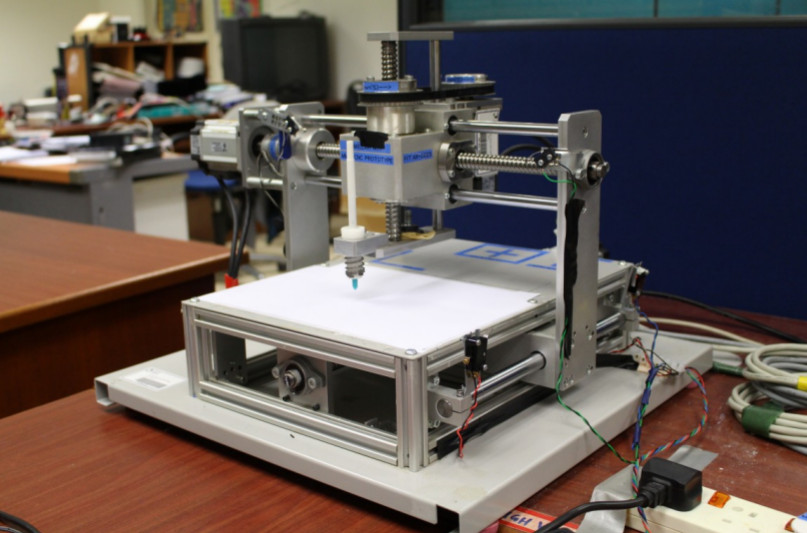
\includegraphics[width=0.85\textwidth]{./07-images/img-Ch4/CNC-Research-Machine-3-Axis.jpg}}
	\caption{The UMP 3-axis CNC Research Machine}
	\label{fig:CNC-Research-Machine-3-Axis.jpg}
\end{center}
\end{figure}

Electrical signal pulses sent to the servo-driver provide information like rotate clockwise (CW), rotate counter-clockwise(CCW), travel distance to rotate, speed to rotate, and so on. The actuation using electrical pulses makes the physical CNC machine instantaneously active. 

% =====================================================
\clearpage
\pagebreak

\begin{figure}[htbp]
	\begin{center}
		\frame{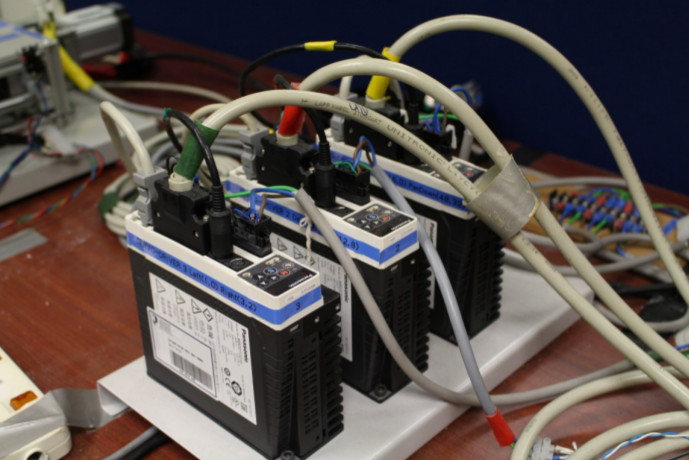
\includegraphics[width=0.73\textwidth]{./07-images/img-Ch4/CNC-Research-Machine-3-Sets-Servo-Drives.jpg}}
		\caption{Servo-Drives for the 3-Axis CNC Research Machine}
		\label{fig:CNC-Research-Machine-3-Sets-Servo-Drives.jpg}
	\end{center}
\end{figure}

\begin{figure}[htbp]
	\begin{center}
		\frame{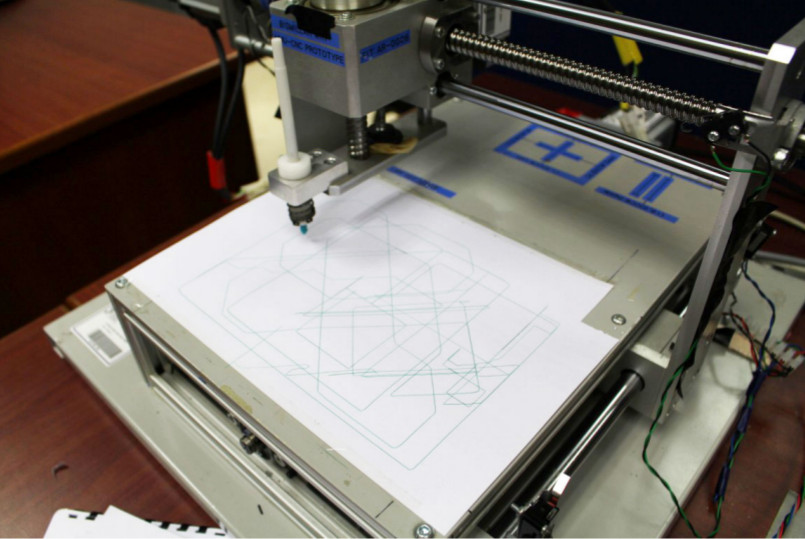
\includegraphics[width=0.73\textwidth]{./07-images/img-Ch4/CNC-Research-Machine-X-Y-Movements.jpg}}
		\caption{CNC Research Machine X-Y Movements}
		\label{fig:CNC-Research-Machine-X-Y-Movements.jpg}
	\end{center}
\end{figure}


For our CNC research machine, we used a commercial, industry standard, Panasonic MINAS A4 AC servo-driver and servo-motor pair. We have three sets of this pair because the research machine is a 3-axis CNC servo driven machine. 
\vspace*{1\baselineskip}

Each Panasonic MINAS A4 servo-motor is a 24-volts, 750-watts, high torque, alternating current (AC) driven motor. It can be configured to operate in a single-phase or a three-phase, AC 60 Hz input current mode.
\vspace*{2\baselineskip}\\

We can configure our CNC research machine to run in three control modes: position control, velocity control, and torque control. It can also be configured either in an open-loop or a closed-loop control scheme.  
\vspace*{1\baselineskip}

The CNC research machine was procured on a joint collaboration project between University Malaysia Pahang (UMP) and Multimedia University, Cyberjaya (MMU), in the year 2008, under the E-Science grant, Ministry of Science, Technology and Environment (MOSTE), Government of Malaysia.  

% =======================
% \clearpage
% \pagebreak

\section{Previous CNC research projects}

We have successfully developed and executed C/C++ software codes using various devices to drive our CNC research machine. We have written codes that combine the following programming techniques: standard serial-running codes, realtime-running codes (RTAI) and parallel-running codes.  
\vspace*{1\baselineskip}

All of the pulse-generator devices that we have used on all of our research projects run C/C++ software codes on the open source Linux platform. On Linux, every software that we need is cost-free and open source. The C/C++ software compiler is cost-free. We even customize the operating system kernel to meet our needs. All of the interpolation computations we accomplished in our projects are of reference-pulse CNC interpolations. 
\vspace*{1\baselineskip}

We avoided the Microsoft (MS) Windows platform because we need full and open access to the operating system and to the software components that control the devices attached to the operating system. In addition, Microsoft Windows operating system is not free. Even, the C/C++ software compiler is not cost-free. In many cases, we cannot find suitable software applications on MS Windows that meets our project needs and that are cost-free. For low-level systems programming (our type of projects), the MS Windows is not a suitable platform for a cost-free development environment.  
% \vspace*{1\baselineskip}

\section{Previous software programming experiences}

On programming experience, we covered realtime execution using RTAI kernel modules on the LinuxCNC system. In the Raspberry Pi 3 project, we managed to drive the CNC system using C++ multi-threading. The concept of RTAI interrupt-style programming architecture can be found in the appendix at [\ref{fig:App4-rtai-architecture-on-linux.jpg}]. 
\vspace*{1\baselineskip}

Examples of realtime codes that we have used in our projects can be found in the appendix at [\ref{App4-Summary main() function C-Code listing for RTAI}], [\ref{App4-Full C-Code listing for Real Time (RTAI)}], and [\ref{App4-Full execution C/C++ code for Real Time (RTAI)}].  
\vspace*{1\baselineskip}

Examples of parallel C/C++-2011 codes using multi-threading can be found in the appendix at [\ref{App4-C++2011 Example Parallel Multithreading}] and [\ref{App4-C++2011 Execution Parallel Multithreading}], while codes for parallel C/C++ MPI (Message Passing Interface) using multi-processing can be found in the appendix at [\ref{App4-C++-MPI Example Parallel Multiprocessing}] and [\ref{App4-C++-MPI Execution Parallel Multiprocessing}]. 
\vspace*{1\baselineskip}

For our research project, we will combine both realtime and parallel codes suitably to meet our CNC machine needs. We will also consider integrating codes or taking ideas from modern and efficient computer programming languages like \href{https://www.rust-lang.org/}{Rust programming language}, with an example multithreading code at [\ref{App4-Rust Parallel Multithreading Codes}] placed in the appendix. Rust is an upcoming low level systems language, a direct competitor to C/C++. Rust was designed from the ground up with Safety, Security and Concurrency (SSC) built-into the Rust engine. This is unlike the C/C++ language or most languages, where these functionality come as separate linked software libraries. More will be discussed in the section on literature review.
\vspace*{1\baselineskip}

Internally, inside the CNC control software we may use \href{https://www.python.org/}{Python programming language} or \href{https://julialang.org/}{Julia programming language} scripts, that have excellent processing and data handling capabilities. These languages support parallel programming internally not through external libraries. This researcher is quite well versed in the use of these computer programming languages. Example codes for Python multithreading and multiprocessing can be found in the appendix at [\ref{App4-Python Parallel Multithreading}] and [\ref{App4-Python Parallel Multithreading}]. And similarly, parallel codes for the Julia language are provided in the appendix at [\ref{App4-Julia Parallel Programming Codes}].
\vspace*{1\baselineskip}

The CNC machine only needs electrical pulses of the right characteristics to run. The kind of devices that generate these electrical pulses does not matter. However, the interface software codes varies between different hardware devices.  
\vspace*{1\baselineskip}

As an example, the full C/C++ software codes that actually generate electrical pulses at the serial and parallel ports of the computer concurrently, is provided in the appendix at this link, [\ref{sec:App4-Write-Parallel-Serial-Ports}]. The named, Concurrent-Writes-to-Parallel-and-Serial-Ports program, is the boundary point (or transition point) where "software codes write bits that finally generate hardware electrical pulses". This bit-writing software program is essentially the CNC Signal Driver software, that in turn takes inputs from the CNC Signal File. The CNC Signal File is, in turn, the output of the complicated work executed by the CNC Interpreter and CNC Interpolator combination, that also in turn, takes its inputs from the G-Code file, which is the starting point of the entire CNC operations. 
\vspace*{1\baselineskip}

Essentially, what we have described above is the "software backward trail" to its starting point in CNC machine operations. From the clarification above, we realize that in order to accomplish this project successfully, from start to finish, software design knowledge, software programming methods and software implementation skills are evidently important.

% \vspace*{1\baselineskip}
% ====================================
% \clearpage
% \pagebreak
\section{Pulse generator devices}

\subsection{Computer extension boards}
The following are projects we have undertaken using pulse generator devices that successfully drive the CNC research machine. For computer extension boards as pulse generator devices, we worked on the following six(6) devices for our research: 
\begin{enumerate}
	\item PC parallel port, [\ref{fig:App4-Captured-Parallel-Port-Built-in-Motherboard.jpg}], [\ref{fig:App4-Captured-Parallel-Port-PCI-Adapter-Card.jpg}], [\ref{fig:App4-Captured-USB-to-Parallel-Port-PL2305-Converter.jpg}].
	
	\item Velleman K8000 Parallel extension board, [\ref{fig:App4-Captured-Velleman-K8000 Parallel-Port-Extension-Board.jpg}].
	
	\item Velleman K8055 USB extension board, [\ref{fig:App4-Captured-Velleman-K8055-USB-Extension-Board.jpg}].
	
	\item Heber X10i USB extension board, [\ref{fig:App4-Captured-Heber-X10i-USB-Extension-Board.jpg}].
	
	\item Arduino Due USB extension board, [\ref{fig:App4-Captured-Arduino-Due-USB-Extension-Board.jpg}].
	
	\item Digilent Nexys-3 Spartan-6 FPGA board. [\ref{fig:App4-Captured-Nexys3-Spartan6-FPGA-USB-Extension-Board.jpg}].
	
\end{enumerate}
 
% \vspace*{1\baselineskip}

\subsection{Single Board Computers}

For single board computers (SBC) as pulse generator devices, we worked on the following three(3) systems for our research: 
\begin{enumerate}
	\item Raspberry Pi SBC, General purpose. [\ref{fig:App4-Captured-Raspberry-Pi3-ModelB-SBC.jpg}], [\ref{fig:App4-Captured-Raspberry-Pi2-ModelB-SBC.jpg}].
	
	\item Banana Pi SBC, Graphic processing focus. [\ref{fig:App4-Banana-PI-M2U-SBC.jpg}].
	
	\item Beagle-Board xM SBC. Graphic processing plus DSP focus. [\ref{fig:App4-Beagle-Board-xM-SBC.jpg}].
	
\end{enumerate}

The above three(3) SBCs all have different brands of processors (CPUs). The Raspberry Pi SBC hardware is suited for general purpose use, while the Banana Pi SBC and BeagleBoard xM SBC are graphic processing focused.
\vspace*{1\baselineskip}

In addition, we have chosen to study Beagle-Board xM  because it has a digital signal processor (DSP) chip, which is not available on both the Raspberry Pi SBC or the Banana Pi SBC.
\vspace*{1\baselineskip}

The primary purpose of all nine(9) devices mentioned above, is to generate electrical pulses through the associated pins on each board. Writing software that generates pulses (high/low for 1/0) at the pins means binary representation in software terms. This is another critical software programming activity in CNC development. 
\vspace*{1\baselineskip}

We need to write software that converts codes into binary formatted strings, for example, generating 8-bit binary strings to drive eight(8) individual parallel lines simultaneously, parallel in time. Similarly, with 16-bit binary strings, we can drive 16 parallel lines simultaneously. Fot that purpose, we provided the full C/C++ program code that converts outputs to 8-bit, 16-bit, and 32-bit binary strings in the appendix at  [\ref{App4-Converting-software-codes-to-binary-bits-pulses}]. 
\vspace*{1\baselineskip}

Even though the binary string generation is common, the actual software driving implementation varies between boards. This arises due to the different pin configurations on each hardware device. We succeeded in our previous projects by manipulating software codes for each board, accordingly.

% \pagebreak
\section{Computer Extension Boards as devices}

\subsection{Project 1 - PC parallel port}

The parallel port hardware in a computer can be a built-in device located on the mother-board or an add-in PCI card attached to the PCI bus of the mother-board. 
\vspace*{1\baselineskip}

There are also converter devices, that converts USB to parallel port, like the Profilic USB to IEEE1284 Bridge Controller Bi-Direction Parallel Interface that uses the PL2305 software driver and is supported on both Windows and Linux. The parallel port software driver must be installed on the Linux computer for software to communicate with it. 
\vspace*{1\baselineskip}

A parallel port control program code written in C/C++ provides commands for the parallel port device (hardware) to generate electrical pulses to drive the CNC machine. The parallel port pins are appropriately connected (wired electrically) to the different servo-drivers of the CNC machine.
\vspace*{1\baselineskip}

The report for this work is at reference \cite{FYP_Abzal_2012}. In this scheme, the various devices connected to the Linux computer are the devices responsible for generating electrical pulses that drives the CNC machine. Images of the parallel port devices that we have used are provided at [\ref{fig:App4-Captured-Parallel-Port-Built-in-Motherboard.jpg}] for parallel port built-in the computer motherboard,  [\ref{fig:App4-Captured-Parallel-Port-PCI-Adapter-Card.jpg}] for the parallel port PCI adapter card and [\ref{fig:App4-Captured-USB-to-Parallel-Port-PL2305-Converter.jpg}] for the USB-to-Parallel port PL2305 converter cable.


\subsection{Project 2 - Velleman K8000 Parallel extension board}

The Velleman K8000 is a computer interface board, a hardware card to control external electrical devices with our computer through the standard parallel cable. The card offers some analog/digital connections to do this.
\vspace*{1\baselineskip}
	
The card is provided with software drivers to run on both Windows and Linux computers. For the K8000 board, software programs on the computer can directly communicate via the parallel protocol IEEE1284 with the board. Software codes can be written in different programming languages like C/C++, Python, VB, Qbasic and Turbo Pascal. 
\vspace*{1\baselineskip}
	
Similarly, a parallel port control program code written in C/C++ provides commands for the parallel port device (hardware) to generate electrical pulses to drive the CNC machine. 
\vspace*{1\baselineskip}
	
The K8000 board digital output pins are appropriately connected (wired electrically) to the different servo-drivers of the CNC machine. On the Velleman K8000 board, the electrical pulses can be seen during CNC execution because LEDs (blinking on and off) are provided for selected pins.
\vspace*{1\baselineskip}

The report for this work is at reference \cite{FYP_Abzal_2012}.	In this scheme, the Velleman K8000 Parallel interface board hardware is the device responsible for generating electrical pulses that drives the CNC machine. The image of the K8000 parallel interface board that we have used is provided at [\ref{fig:App4-Captured-Velleman-K8000 Parallel-Port-Extension-Board.jpg}].

\subsection{Project 3 - Velleman K8055 USB extension board}

The Velleman K8055 board is a USB extension board that has 5 digital input channels and 8 digital output channels. There are two analogue inputs and two analogue outputs with 8 bit resolution. The number of inputs and outputs can be further expanded by connecting up to a maximum of four K8055 cards. 
\vspace*{1\baselineskip}

The board is provided with software drivers to run on both Windows and Linux computers. For the K8055 board, software programs on the computer can directly communicate via the USB protocol with the board. It is like driving a typical USB printer. Software codes can be written in different programming languages like C/C++, Delphi, Python, Visual Basic, Qbasic and Turbo Pascal.
\vspace*{1\baselineskip}

Similarly, a USB port control program code written in C/C++ provides commands for the USB port device (hardware) to generate electrical pulses to drive the CNC machine. The K8055 board digital output pins are appropriately connected (wired electrically) to the different servo-drivers of the CNC machine. Also on the Velleman K8055 board, the electrical pulses can be seen during CNC execution because LEDs (blinking on and off) are provided for selected pins.
\vspace*{1\baselineskip}

The report for this work is at reference \cite{FYP_Rajeef_2015}. In this scheme, the Velleman K8055 USB interface board hardware is the device responsible for generating electrical pulses that drives the CNC machine. The image of the K8055 USB interface board that we have used is provided at [\ref{fig:App4-Captured-Velleman-K8055-USB-Extension-Board.jpg}]. 

\subsection{Project 4 - Heber X10i USB extension board}

The Heber X10i USB Board is also an extension board connected to the Linux computer via the USB port. The Heber X10i software driver must be installed on the Linux computer for software to communicate with it. The Heber board digital output pins are connected (wired electrically) to appropriate servo-drivers for the 3-axis CNC machine. 
\vspace*{1\baselineskip}

For the Herber board, software programs written in C/C++ on the Linux machine can directly communicate via USB with the board. It is like driving a typical USB printer. 
\vspace*{1\baselineskip}

As an extension board, there is no need for a compiled firmware to be downloaded onto the Heber board. Software instructions to generate electrical pulses come directly from the C/C++software programs on the Linux computer. Software codes can be written in different programming languages like C/C++ and Python.
\vspace*{1\baselineskip}

The report for this work is at reference \cite{FYP_Saleh_2014}. In this scheme, the Heber X10i USB Board is the device responsible for generating electrical pulses. The image of the  Heber X10i USB board that we have used is provided at [\ref{fig:App4-Captured-Heber-X10i-USB-Extension-Board.jpg}].


\subsection{Project 5 - Arduino Due USB extension board}

The Arduino Due board is an extension board connected to the Linux computer via the USB port. The Arduino Due software driver must be installed on the Linux computer for software to communicate with it. 
\vspace*{1\baselineskip}

A control program written in C/C++ on the Linux machine is compiled to produce machine codes (basically firmware) that is downloaded and installed into the memory of the Arduino Due board. 
\vspace*{1\baselineskip}

For the Arduino Due board, software programs on the computer cannot directly communicate online with the board. When any changes made in the software code to drive the CNC machine, it has to be recompiled and re-downloaded to the Arduino Due memory. This is different from the driving schemes in both Velleman K8000, Velleman K8055 and Heber X10i boards, where control programs on the Linux machine can directly drive electrical pulses through the boards to the CNC machine. 
\vspace*{1\baselineskip}

The relevant digital output pins on the Arduino Due are appropriately connected (wired electrically) to the CNC machine. 
\vspace*{1\baselineskip}

The report for this work is at reference \cite{FYP_Hazmi_2014}. In this scheme, the Arduino Due USB Board is the device responsible for generating electrical pulses. The image of the  Arduino Due USB board that we have used is provided at [\ref{fig:App4-Captured-Arduino-Due-USB-Extension-Board.jpg}].

% \pagebreak
\subsection{Project 6 - Digilent Nexys-3 Spartan-6 FPGA USB board}

The FPGA (Field Programmable Gate Array) USB board is also an extension board connected to the Linux computer via the USB port. The FPGA board software driver must be installed on the Linux computer for software to communicate with it.
\vspace*{1\baselineskip}

FPGAs are semiconductor devices comprising programmable logic blocks and interconnection circuits. It can be programmed or re-programmed to the required functionality after manufacturing. Programming FPGA generates firmware. It was said that FPGA is about using software to program hardware.
\vspace*{1\baselineskip}

The FPGA firmware for the Nexys-3 Spartan-6 FPGA, is a compiled VHSIC Hardware Description Language (VHDL) software on the Linux computer. After compilation it is downloaded onto the FPGA board to control the board. 
\vspace*{1\baselineskip}

The FPGA board digital output pins are connected with wires to appropriate servo-drivers for the 3-axis CNC machine. 
\vspace*{1\baselineskip}

After installation of the firmware on the FPGA board, software program instructions written in C/C++ on the Linux machine can directly communicate via USB with the board. With these received instructions, the FPGA pins appropriately generate the required electrical pulses to the CNC machine. 
\vspace*{1\baselineskip}

The Nexys-3 FPGA hardware development board manufactured by Digilent Inc. This board was used to control the CNC machine using its programmable input/output (I/O) pins. This hardware is a USB extension board to the Linux computer. The board was installed with a set of software drivers for the Linux platform.
\vspace*{1\baselineskip}

A linux based personal computer running Ubuntu 10.04 LTS (Long Term Support) with RTAI (Real Time Application Interface) was deployed. The linux kernel version was linux-2.6.32-122-rtai, and was installed as part of the LinuxCNC system.   
\vspace*{1\baselineskip}

The FPGA board is an external control board connected to the linux computer via a USB port. The FPGA board pins were then connected with wires to appropriate servo-drivers for the 3-axis CNC machine. 
\vspace*{1\baselineskip}

The Xilinx ISE ver. 14.7 software application was used to generate the FPGA firmware. The FPGA firmware program was written using VHSIC Hardware Description Language (VHDL) language. VHDL is a hardware description language used in electronic design automation to describe digital and mixed-signal systems such as field-programmable gate arrays (FPGA) and integrated circuits (ICs). 
\vspace*{1\baselineskip}

VHDL is hardware programming using software, that results in firmware. Firmware is loaded into hardware to make the hardware work, basically controls the hardware. VHDL is inherently a general purpose parallel programming language. A VDHL program source code was created on the personal computer. The Xilinx ISE application compiles this VDHL code into a firmware code we called (FPGA-NEXYS3). This generated firmware was then uploaded from the computer into the FPGA board. Now the board is ready for use with our CNC machine. 
\vspace*{1\baselineskip}

Essentially, the VHDL programming that was carried out to produce the FPGA-NEXYS3 firmware code is to map FPGA parameters and hardware pins for connections to servo-drivers for the 3-axis CNC machine. The G-Code File Interpreter (GFI) software was developed on the Linux platform. The Signals File Sender (SFS) software was developed on the Linux platform using C/C++ code. 
\vspace*{1\baselineskip}

It is important to note that in this FPGA research project, it is the combination of three(3) components: the GFI, the SFS and the FPGA-NESYS3 firmware that drive the CNC machine. First, a RS274D NGC G-Code file is processed by the GFI program to produce a signals file. Next, the SFS program transmits the contents of this signals file to the FPGA board. 
\vspace*{1\baselineskip}

The FPGA board with ready loaded-to-use FPGS-NEXYS3 firmware automatically sends separate electronic signals (pulses) in parallel to the individual servo-drives of the 3-axis CNC machine.
\vspace*{1\baselineskip}

The report for this work is at reference \cite{FYP_Charles_2014}. In this scheme, the Nexys-3 Spartan-6 FPGA USB Board is the device responsible for generating electrical pulses to drive the CNC machine. The image of the  FPGA USB board that we have used is provided at [\ref{fig:App4-Captured-Nexys3-Spartan6-FPGA-USB-Extension-Board.jpg}].

% ==========================================
% \clearpage
% \pagebreak

\section{Single Board Computers as devices}

\subsection{Project 7 - Raspberry Pi 2 and Raspberry Pi 3 SBC boards}

The Raspberry Pi 3 Model B, is a cheap, tiny credit card size, full-fledged computer system that can run software applications. It is called a Single Board Computer (SBC). The Raspberry Pi 2 is similar to Raspberry Pi 3, but is has less memory, less CPU speed (GHz), less USB ports, and less in everything. However, it works the same. This SBC is based on the ARM CPU processor and not the Intel CPU processor. This SBC includes built LAN and wireless networking. 
\vspace*{1\baselineskip}

The SBC (single board computer) is a true full-fledged computer in itself. It is not an extension board to some computer. The SBC is like a "desktop" computer that requires external peripherals. To use this Raspberry Pi SBC, we need just connect a keyboard, mouse, display monitor, power supply, and a micro SD card with an installed Linux Distribution, in a manner similar to connecting the same peripherals to the desktop computer. 
\vspace*{1\baselineskip}

With an operating system like Raspbian (Ubuntu-based) installed, we have full fledged Linux capabilities on the Raspberry Pi, including all software applications and language compilers available for Linux Ubuntu. The required software drivers, for example, BCM2835 must be installed to access specified components and peripherals on the Raspberry Pi.
\vspace*{1\baselineskip}

The Raspberry Pi digital output pins are connected with wires directly to appropriate servo-drivers for the 3-axis CNC machine. Software programs written in C/C++, residing on the Raspberry Pi can directly drive electrical pulses through the digital output pins to the CNC machine. There is no need for any other computer.
\vspace*{1\baselineskip}

The report for this work is at reference \cite{FYP_Asyrul_2017}. In this scheme, the Raspberry Pi-3 Model-B SBC is the device responsible for generating electrical pulses to drive the CNC machine. 
\vspace*{1\baselineskip}

The image of the  Raspberry Pi-3 Model-B that we have used is provided at [\ref{fig:App4-Captured-Raspberry-Pi3-ModelB-SBC.jpg}] and for the Raspberry Pi-2 Model-B is provided at [\ref{fig:App4-Captured-Raspberry-Pi2-ModelB-SBC.jpg}]. The image comparison between Raspberry Pi-3 and Raspberry Pi-2 is provided at [\ref{fig:App4-Captured-Raspberry-Pi2-ModelB-SBC.jpg}].
% \vspace*{1\baselineskip}

\subsection{Project 8 - Banana Pi BPI-M2 SBC board}

Banana Pi BPI-M2 Ultra is a quad-core mini single board computer built with Allwinner R40 SoC. It features 2GB of RAM and 8GB eMMC. It also has onboard WiFi and BT. On the ports side, the BPI-M2 Ultra has 2 USB A 2.0 ports, 1 USB OTG port, 1 HDMI port, 1 audio jack, a DC power port, and last but not least, a SATA port.
\vspace*{1\baselineskip}

Also being a member of the Banana Pi family, the M2 Ultra is a direct upgrade from the Banana Pi M1/M1+ that support SATA from the SoC. The SATA performance on the R40 is fitting for media related projects such as storage servers. Backed by our community, starting a project and building servers is fun and rewarding. 
\vspace*{1\baselineskip}

The Banana Pi operating system is similar to the Raspberry Pi, but a modified version to suit its hardware. It uses the same Raspbian system based on the Ubuntu software for desktops and notebooks. Software C/C++ programming is the same as for the Raspberry Pi. The only difference is the software driver for devices on the board. Raspberry Pi uses different hardware chips on its board compared to the Banana Pi, basically their product differentiations and marketing strategy.  
\vspace*{1\baselineskip}

The report for this work is at reference \cite{FYP_Rajeef_2015}. In this scheme, the Banana Pi BPI-M2 SBC is the device responsible for generating electrical pulses to drive the CNC machine. The image of the Banana Pi BPI-M2 SBC that we have used is provided at [\ref{fig:App4-Banana-PI-M2U-SBC.jpg}].

\subsection{Project 9 - Beagle-Board xM SBC board}

The BeagleBoard is a pocket-sized reference board containing a Texas Instruments Open Multimedia Application Platform (OMAP) 3 system-on-a-chip (SoC) processor, which includes an ARM Cortex-A8 core, Texas Instruments C64x+ digital signal processor (DSP), and onboard graphics engine, as well as integrated dual data rate (DDR) random-access memory (RAM). The BeagleBoard is an inexpensive platform for hobbyists, academics, and professionals who are learning Linux and small systems.
\vspace*{1\baselineskip}

We chose this BeagleBoard xM for research because it has a digital signal processor (DSP), which is not available on the Raspberry Pi SBC or the Banana Pi SBC.
\vspace*{1\baselineskip}

Similarly, the Beagle-Board xM operating system is similar to the Raspberry Pi, but a modified version to suit its hardware. It uses the same Raspbian system based on the Ubuntu software for desktops and notebooks. Software C/C++ programming is the same as for the Raspberry Pi. The only difference is the software driver for devices on the board. Raspberry Pi uses different hardware chips on its board compared to the Beagle-Board xM, basically their product differentiations and marketing strategy.  The report for this work is at reference \cite{FYP_Rajeef_2015}. In this scheme, the Beagle-Board xM SBC is the device responsible for generating electrical pulses to drive the CNC machine. The image of the Beagle-Board xM SBC that we have used is provided at [\ref{fig:App4-Beagle-Board-xM-SBC.jpg}].

\pagebreak
%% =========================================================
\section{Summary on Related Research Work}
%% =========================================================

We started by providing a brief description of our UMP CNC Research machine, a 3-axis experimental CNC router-type machine, that instead of using a tool cutter, uses a pen to create drawings on paper in the X-Y plane. We also showed images of the CNC Research machine. Each axis of the machine is driven by an alternating current servo-driver and servo-motor pair. The servo-driver can be driven using 3 different control strategies: position control, velocity control and torque control.
\vspace*{1\baselineskip}

Next, we mentioned that only C/C++ software codes were used on various hardware devices as pulse generators to drive the CNC Research machine. The written codes include combinations of standard serial-running codes, realtime-running codes (RTAI) and parallel multi-threaded running codes.  
\vspace*{1\baselineskip}

We ran the C/C++ software codes on the open source Linux platform only. We avoided the Microsoft (MS) Windows platform because it is not possible to get full and open access to the operating system environment, that is, to the hardware devices attached to the operating system. We concluded that the MS Windows environment is not a suitable platform for our specific research project.  
\vspace*{1\baselineskip}

All of the interpolation computations we accomplished in our projects are of reference-pulse type CNC interpolations. We also implemented both non-realtime and realtime executions on the CNC Research machine.
\vspace*{1\baselineskip}

Since the CNC machine only needs electrical pulses of the right characteristics to run, the kind of devices that generate these electrical pulses does not matter. On this matter, we described the hardware pulse generator devices comprising of six(6) computer extension board devices and three(3) single board computers (SBC) that we have successfully implemented in driving the CNC Research machine.
\vspace*{1\baselineskip}

For driving the CNC Research machine using the parallel port, the four(4) devices used comprised, the built-in parallel port on the computer motherboard, the parallel port PCI adapter card, the USB-to-Parallel port PL2305 converter cable and the Velleman K8000 Parallel extension board.
\vspace*{1\baselineskip}

For driving the CNC Research machine using the USB port, the four(4) devices used comprised, the Velleman K8055 USB extension board, the Heber X10i USB extension board, the Arduino Due USB extension board, and the Digilent Nexys-3 Spartan-6 FPGA USB development board.
\vspace*{1\baselineskip}

For driving the CNC Research machine using standalone Single Board Computers (SBC), the four(4) devices used comprised, the Raspberry Pi 2 and Raspberry Pi 3 SBC boards, the Banana Pi BPI-M2 SBC board, and the Beagle-Board xM SBC board. 
\vspace*{1\baselineskip}

In the Appendix for Chapter-4 at this link [\ref{sec:App4-Related-Research-Work}], we included some results on our previous CNC research. Following that, we included images and specifications of the various hardware pulse generator devices we have successfully implemented on our CNC Research machine. And we included full contents of realtime and parallel running software codes, as examples.



% ==========================================================

%	\pagebreak
\begin{tcolorbox}
	
\section{zzAdvice-on-Chapter-4}

\textbf{RELATED RESEARCH WORK}
\vspace*{1\baselineskip}

\textbf{Chapter 4 Guidelines - TO REMOVE LATER}	
\vspace*{1\baselineskip}

\begin{enumerate}
	
	\item contains a concise outline of the work you have carried out so far and of the progress you have made toward the aims of the project.
	
	\item should concentrate on the parts that contribute specifically to the goals of  proposal,
	
	\item avoiding detailed descriptions of digressions you may have attempted in the earlier, more exploratory, phases of your work.
	
	\item if you have already obtained preliminary results, this is the chapter where you should provide them, in a structured manner that helps supporting the rest of the proposal.
	

\end{enumerate}
	
\end{tcolorbox}



\titleformat {\chapter} {\normalfont\huge\bfseries\color{black}}   {\thechapter}{10pt}{\huge} 
\chapter {Research Implementation Plan}

\section{Main Tasks in Research Implementation Plan}

The total estimated duration for this research project is 356 days or about 1 calendar year. As shown in the figure below, the project tasks have been separated into four main categories as follows:
\begin{enumerate}
	\item Project Preliminaries and Setup (Task No. 2 until Task No. 117)
	\item Software Design and Implementation (Task No. 146 until Task No. 178) 
	\item Software Testing and Reporting (Task No. 190 until Task No. 219) 
	\item Project Publication and Closing (Task No. 224 until Task No. 233) 
\end{enumerate}

\begin{figure}[htbp]
	\begin{center}
		\frame{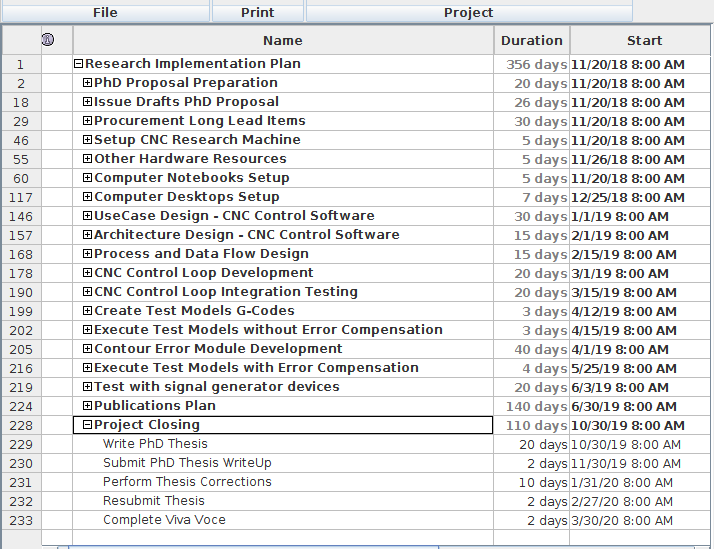
\includegraphics[width=0.95\textwidth]{./07-images/img-Ch5/00-Research-Implementation-Plan.png}}
		\caption{Main Tasks in Research Implementation Plan}
		\label{fig:00-Research-Implementation=Plan.png}
	\end{center}
\end{figure}

The Work Breakdown Structure (WBS) or subtasks with details for the Research Implementation Plan are provided in the appendix at the link Fig [~\ref{sec:App5-Research-Implementation-Plan}].

%%\vspace{0.5cm}
%%\vspace{0.5cm}

%% =================================================
\clearpage
\pagebreak
\begin{landscape}

\section{Overview of Research Implementation Schedule}

\begin{figure}[htbp]
	\begin{center}
		\frame{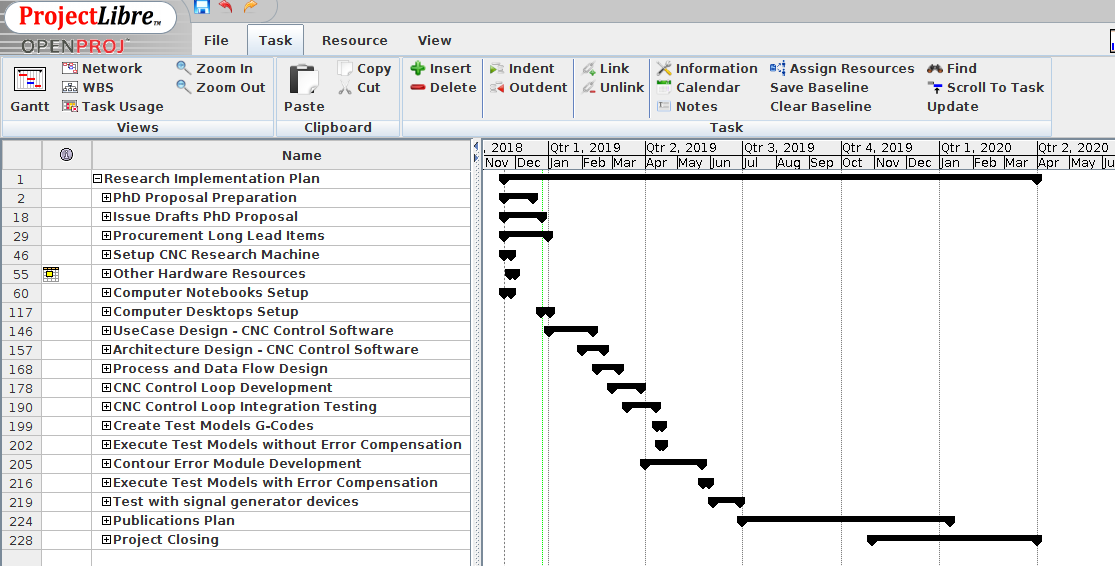
\includegraphics[width=1.35\textwidth]{./07-images/img-Ch5/Overview-Research-Implementation-Plan.png}}
		\caption{Overview of Research Implementation Schedule}
		\label{fig:Overview-Research-Implementation-Plan.png}
	\end{center}
\end{figure}

\end{landscape}

%% =================================================

\section{Critical Project Tasks} 
The identified critical tasks are the UseCase Design, Architecture Design, Process and Data Flow Design, and the Control Loop Design.
\vspace{0.5cm}

The UseCase design must be correct and complete covering all possibilities of system usage, link at [~\ref{sec:App5-UseCase Design}]. UseCases are the blueprint for software design. Incomplete UseCases may cause missing features and functions in the software. The software architecture, process flow, data flow and control loop designs, link at [~\ref{sec:App5-Process-Flow Design}], must ensure that the system will be built with flexible and upgradeable features. A design that is incomplete and rigid may require a complete design rework if certain new features need to be added or existing features need to be modified.	
\vspace{0.5cm}
	
Since software design is the blueprint for software construction, good design facilitates good software construction. In this project, we anticipate a few rounds of iterative designs since software construction will be conducted following the incremental and prototyping model. This software construction method saves time and eliminates complex logical design errors. In the incremental and prototyping model, the system is developed by starting from having small features, then incrementally built, tested, and then reworked as necessary until an acceptable complete system is achieved. This model works best where not all of the project requirements are known in detail ahead of time. This process development model is iterative, sort of, a trial-and-error process that repeats until the final design goals have been achieved. 
	
\section{Research Milestones}
The project milestones follow closely the project critical tasks. Successful completion of usecases, software architecture, process flow, data flow and control loop designs are the five primary milestones in this research project. Successful completion of control loop testing, integrated testing, hardware system testing and publication submissions are another four secondary milestones in this project.  
%% \vspace{0.5cm}
	
\section{Publications Plan}

We anticipate a total of three publications spread three months apart in this research project. The target is two conference publications and one journal publication. The first conference publication will be for the Pico Universal PWM hardware with LinuxCNC, and the second publication will be for the Microchip MCU Curiosity and 28-Pin LIN development boards and the CNC Control Software. The target journal publication will be for CNC Interpolation, which is the main thesis for this research.

% ======================================================	
\section{Implementation approach}
% ======================================================

The implementation approach is to focus on the utilization of modern software engineering technologies like efficient data structures, fast algorithms, realtime and parallel computations, tractable program executions, integrations of different programming language libraries and many more that will be explored during the software design stage. The final goal is to achieve an efficient implementation for a realtime and parallel look-ahead control and feedrate compensation strategy for CNC reference-pulse interpolation.

%% =====================================================	

%	\pagebreak
%% ===========================================
\begin{tcolorbox}
	
\section{zzAdvice-on-Chapter-5}

\textbf{RESEARCH IMPLEMENTATION}
\vspace*{1\baselineskip}

\textbf{Chapter 5 Guidelines - TO REMOVE LATER}	
\vspace*{1\baselineskip}	
	
\subsection{Implementation Schedule - Gantt Chart}

Depth of plans - Not all research proposals lend themselves easily to the creation of detailed work plans. In some cases, namely when the work fits the broader plans of a research group that is progressing steadily, it is possible do build a detailed description of 

what the researcher plans to do (literature to explore in depth, principles or theorems to formulate and prove, experiments to carry out, sub-systems to build, systems integrations to perform, tests to accomplish).

Define and List the tasks

\subsection{Critical Tasks} 

Identify Critical Tasks, why critical. Focus. Plan to tackle problems. The plan should anticipate the problems likely to be found along the way and describe the approaches to be followed in solving them.

\subsection{Research Milestones}

Plan the tasks - In these cases, it is possible, and desirable, to establish specific milestones and time lines and a Gantt diagram. Identify critical tasks.

\subsection{Publications Plan}

Plan for publications - It should also anticipate the conferences and journals to which the work in progress is expected to be submitted along the way, and schedule it in a Goals for Publication section of the work plan.

Focus - In spite of its contingency, this list may work marvels in keeping the researcher focused, motivated and beneficially under pressure.

\section{Expected Results}

\textbf{Result oriented} - Whatever its nature, comprehensive or sketchy, your work plan should be able to put in perspective the implications of the successive steps of your work, reinforcing, in the mind of the reader, the conviction that your approach is solidly oriented toward results, that the topic is timely and relevant, and that the outcomes of the project will contribute significantly to the enhancement of the field.

	
	
\end{tcolorbox}



\titleformat {\chapter} {\normalfont\huge\bfseries\color{black}}   {\thechapter}{10pt}{\huge} 
\chapter {Conclusion}

%% Bismillah Hirrahma Nirrahim

The focus of this research is CNC interpolation. Technically, CNC interpolation is about the task of generating and sending signal pulses to the respective electric motors at the machine's axis-of-motions, in a coordinated and timely manner, such that the machine tool accurately tracks the desired contour path in the move from the current position to the next position. 
\vspace{0.5cm}

To achieve the task, the interpolator must generate the right number of signal pulses that achieves the desired distance for the move, and drive the correct pulse feedrate (frequency) that achieves the desired velocity for the move.	
\vspace{0.5cm}

This research emphasizes the adoption of effective and efficient software engineering technologies in the implementation details of CNC interpolation. The adoption includes sophisticated data structures, efficient process and data flow algorithms, high resolution realtime monitoring, true parallel executions, thread-safe process designs, high speed data dumps (captures), signal/slot programming mechanism and many more deployment techniques that can be creatively developed with modern software compilers available today. 
\vspace{0.5cm}

Software program control paradigms considered for the CNC Control Loop include process-driven, interrupt-driven, target-driven and optimal-driven methods. Software integration strategies considered include the utilization of back end packages and libraries like Scilab-NURBS, Octave-NURBS, Rust low-level thread safe constructs, Julia and Python parallel libraries over and above the C/C++ base program codes. This program control is the core activity for this research. 
\vspace{0.5cm}

All software implemented in this research are open source, cost-free, and actively supported by the software community. This facilitates sharing of knowledge, software solutions, programming tricks and passionate lifelong learning.
\vspace{0.5cm}

For performance comparisons, hardware architectures comprising both 64bit and 32bit systems with different configurations will be used. In addition, three different pulse generator devices will be deployed in this research project. 
\vspace{0.5cm}

The ultimate goal is to suitably implement selected software technologies that achieves our primary research target, that is, a realtime and parallel look-ahead control and feedrate compensation for the CNC reference-pulse interpolation task. For this research, the other target is to produce two conference papers and a journal paper.
\vspace{0.5cm}

This proposal is an exciting and exhilarating research project, especially for a software engineer. However, success can be elusive. On that note, it is our firm belief that the eventual success of this research rests on the help and inspiration from Allah, the All Mighty, the Most Gracious and Most Merciful. In this endeavor, we pray to Allah for his continuous blessings.
\vspace{0.5cm}

%% ==============================================	
%	\pagebreak
%% ===========================================
\begin{tcolorbox}
	
\section{zzAdvice-on-Chapter-6}

\textbf{CONCLUSION}
\vspace*{1\baselineskip}

\textbf{Chapter 6 Guidelines - TO REMOVE LATER}	
\vspace*{1\baselineskip}
	
The Conclusions should 
	
	\begin{enumerate}
		\item briefly restate the objectives of your research project, 
		\item recap the research approach you plan to follow, 
		\item clarify in a few words what you expect to find out, 
		\item explain why it is scientifically valuable to find it out, 
		\item describe on what basis you expect to evaluate the validity of your results.
	\end{enumerate}
	
\end{tcolorbox}



%% =======================================
% THE BIBLIOGRAPHY (REFERENCES)
% IN TEXSTUDIO file:///usr/share/doc/texstudio/html/latex2e.html#Using-BibTeX

% STYLESHEET /usr/share/texlive/texmf-dist/bibtex/bst/base/acm.bst
% \bibliographystyle{acm}  
% \bibliography{./03-bib-files/Bibliography-List-ACM} %% Using FILE Bibliography-List-ACM

% STYLESHEET /usr/share/texlive/texmf-dist/bibtex/bst/base/ieeetr.bst
\bibliographystyle{ieeetr}  %% Using STYLE ieeetr.bst
\bibliography{./03-bib-files/References}   %% Using FILE References.bib FOR ENTRIES

% FOR APPENDIX FOR EACH = IMPORTANT
\appendix
\renewcommand{\thechapter}{\arabic{chapter}}
\chapter{Appendices}

The contents of the appendices are organized according to chapters presented in the main text. The appendices are as listed as follows: The link to directly jump to each appendix is also provided.

\begin{enumerate}[start=1,label={(\bfseries \arabic*):}]
	\item Chapter-1 Appendices (Introduction) [\ref{sec:App1-Introduction}] 
	\item Chapter-2 Appendices (Literature Survey)[\ref{sec:App2-Literature-Survey}] 
	\item Chapter-3 Appendices (Research Methodology)[\ref{sec:App3-Research-Methodology}] 
	\item Chapter-4 Appendices (Related Research Work)[\ref{sec:App4-Related-Research-Work}] 
	\item Chapter-5 Appendices (Research Implementation Plan)[\ref{sec:App5-Research-Implementation-Plan}] 
\end{enumerate}

\clearpage
\pagebreak

%% SEPARATE FILES AS INPUT
% ==========================================================
\clearpage
\pagebreak
\justifying
\renewcommand{\thesection}{A \arabic{section}}

\titleformat{\section}{\normalfont\LARGE\bfseries\color{black}}{\thesection}{10pt}{\LARGE}
\section{Appendix-A1 Introduction}\label{sec:App1-Introduction}

% ==========================================================	
\subsection{App1-CNC Milling Machine}
\begin{figure}[htbp]
	\begin{center}
		\frame{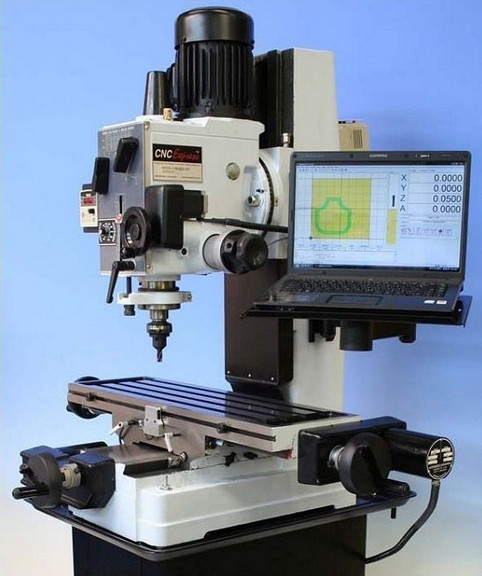
\includegraphics[width=0.5\textwidth]{./07-images/img-Ch1App/CNC-Milling-Machine.jpg}}
		\caption{App1-CNC Milling Machine}
		\label{fig:App1-CNC-Milling-Machine.jpg}
	\end{center}
\end{figure}

% ==========================================================
\subsection{App1-CNC Lathe Machine}
\begin{figure}[htbp]
	\begin{center}
		\frame{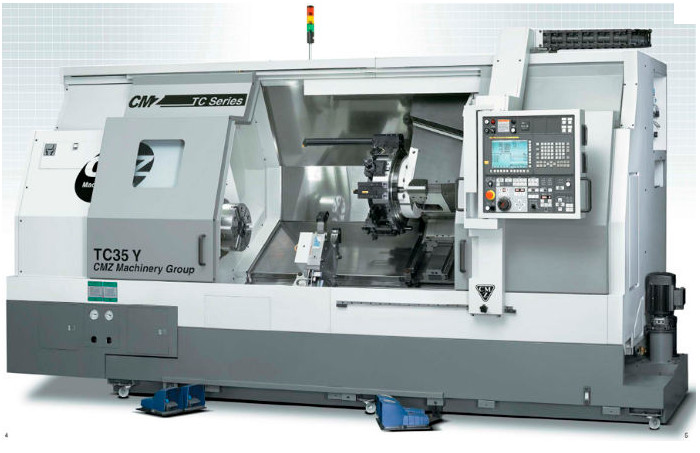
\includegraphics[width=0.5\textwidth]{./07-images/img-Ch1App/CNC-Lathe-Machine.jpg}}
		\caption{App1-CNC Lathe Machine}
		\label{fig:App1-CNC-Lathe-Machine.jpg}
	\end{center}
\end{figure}

% ==========================================================
\clearpage
\pagebreak
\subsection{App1-CNC Routing Machine}
\begin{figure}[htbp]
	\begin{center}
		\frame{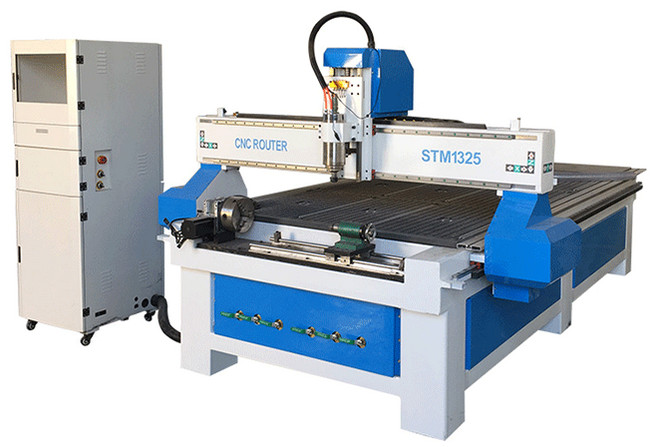
\includegraphics[width=0.50\textwidth]{./07-images/img-Ch1App/CNC-Routing-Machine.jpg}}
		\caption{App1-CNC Routing Machine}
		\label{fig:App1-CNC-Routing-Machine.jpg}
	\end{center}
\end{figure}

% ===========================================================
\subsection{App1-CNC 3D Printing Machine}
\begin{figure}[htbp]
	\begin{center}
		\frame{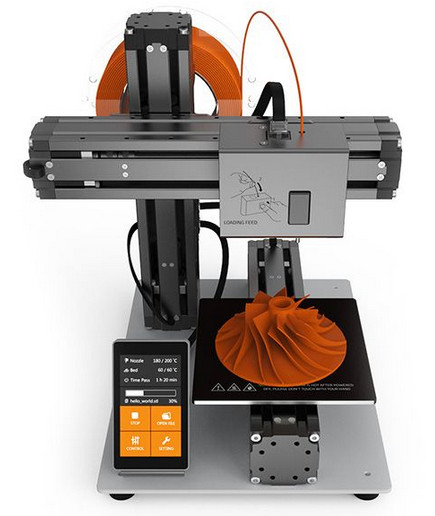
\includegraphics[width=0.5\textwidth]{./07-images/img-Ch1App/CNC-3D-Printing-Machine.jpg}}
		\caption{App1-CNC 3D Printing Machine}
		\label{fig:App1-CNC-3D-Printing-Machine.jpg}
	\end{center}
\end{figure}

% ==========================================================
 %% Introduction
% ==========================================================
\clearpage
\pagebreak
\justifying
\renewcommand{\thesection}{B \arabic{section}}

\titleformat{\section}{\normalfont\LARGE\bfseries\color{black}}{\thesection}{10pt}{\LARGE}
\section{Appendix-B2 Literature Survey}\label{sec:App2-Literature-Survey}

% ==========================================================
\clearpage
\begin{landscape}
\subsection{App2-Ha Scilab NURBS versus Octave NURBS}
	
	\begin{table}[ht]
		\begin{center}
			\caption{App2-Scilab NURBS versus Octave NURBS}		
			\label{table:App2-Scilab NURBS versus Octave NURBS}	
			
			\begin{tabular}{ |p{0.5cm}|p{5.0cm}|p{9.0cm}|p{9.0cm}|}
				\rowcolor{gray!10}			
				\hline \multicolumn{4}{|c|}{\textbf{Scilab NURBS versus Octave NURBS}} \\ [1.0ex]
				\rowcolor{gray!10}
				\hline \textbf{No} & \textbf{Specifications}    & \textbf{Hewlett Packard EliteBook 8470p} & \textbf{Hewlett Packard ProBook 440G}\\ 
				
				\hline 1 & Name of Student    & Wan Ruslan bin W Yusoff & hello\\ 
				\hline 2 & Student ID         &  aaa & Hello\\ 
				\hline 3 & National Reg. ID   & bbb  & Hello\\ 
				\hline 4 & Faculty            & ccc  & Hello\\ 
				
				\hline
			\end{tabular}
		\end{center}
	\end{table}  
	
	
\end{landscape}
% ==========================================================
% ==========================================================
\clearpage
\begin{landscape}
	\subsection{App2-Scilab NURBS versus Octave NURBS}
	
	\begin{table}[ht]
		\begin{center}
			\caption{App2-Computer Notebook Specifications}		
			\label{tabl2:App2-Computer Notebook Specifications}	
			
			\begin{tabular}{ |p{0.5cm}|p{5.0cm}|p{9.0cm}|p{9.0cm}|}
				\rowcolor{gray!10}			
				\hline \multicolumn{4}{|c|}{\textbf{Computer Notebook Specifications}} \\ [1.0ex]
				\rowcolor{gray!10}
				\hline \textbf{No} & \textbf{Specifications}    & \textbf{Hewlett Packard EliteBook 8470p} & \textbf{Hewlett Packard ProBook 440G}\\ 
				
				\hline 1 & Name of Student    & Wan Ruslan bin W Yusoff & hello\\ 
				\hline 2 & Student ID         &  aaa & Hello\\ 
				\hline 3 & National Reg. ID   & bbb  & Hello\\ 
				\hline 4 & Faculty            & ccc  & Hello\\ 
				
				\hline
			\end{tabular}
		\end{center}
	\end{table}  
	
	
\end{landscape}
% ==========================================================
% ==========================================================

\clearpage
\begin{landscape}
	\subsection{App2-Bla bla bla}
	
	\begin{table}[ht]
		\begin{center}
			\caption{App2-Computer Notebook Specifications}		
			\label{table:App2-Computer Notebook Specifications}	
			
			\begin{tabular}{ |p{0.5cm}|p{5.0cm}|p{9.0cm}|p{9.0cm}|}
				\rowcolor{gray!10}			
				\hline \multicolumn{4}{|c|}{\textbf{Computer Notebook Specifications}} \\ [1.0ex]
				\rowcolor{gray!10}
				\hline \textbf{No} & \textbf{Specifications}    & \textbf{Hewlett Packard EliteBook 8470p} & \textbf{Hewlett Packard ProBook 440G}\\ 
				
				\hline 1 & Name of Student    & Wan Ruslan bin W Yusoff & hello\\ 
				\hline 2 & Student ID         &  aaa & Hello\\ 
				\hline 3 & National Reg. ID   & bbb  & Hello\\ 
				\hline 4 & Faculty            & ccc  & Hello\\ 
				
				\hline
			\end{tabular}
		\end{center}
	\end{table}  
	
	
\end{landscape}
% ==========================================================
% ========================================================== %% Literature Survey
% ==========================================================
\clearpage
\pagebreak
\justifying
\renewcommand{\thesection}{C \arabic{section}}

\titleformat{\section}{\normalfont\LARGE\bfseries\color{black}}{\thesection}{10pt}{\LARGE}
\section{Appendix-C3 Research Methodology}\label{sec:App3-Research-Methodology}

% ==========================================================
\subsection{App3-Pico Universal PWM Servo Controller}\label{sec:C-3.1-Universal PWM Servo Controller Board}
				
\begin{figure}[htbp]
	\begin{center}
		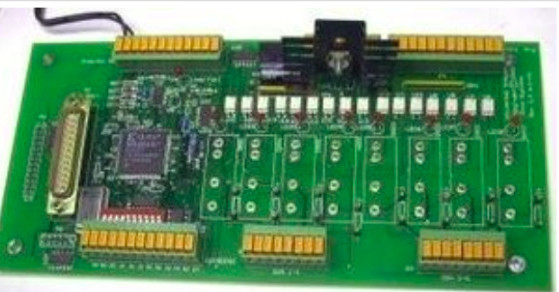
\includegraphics[width=0.85\textwidth]{./07-images/img-Ch3App/Universal-PWM-Servo-Controller.jpg}
		\caption{App3-Universal PWM Servo Controller Parallel Port Interface Board}
		\label{fig:App3-Universal-PWM-Servo-Controller.jpg}
	\end{center}
\end{figure}

\subsection{App3-Specifications Pico Universal PWM Servo Controller}

Reference: \url{http://www.pico-systems.com/motion.html}
\vspace{0.5cm}

The Universal PWM Servo Controller is a small board with everything needed to control a 2-axis, 3-axis or 4-axis machine tool with PWM-driven servo amplifiers. It contains 4 PWM generators with variable PWM drive frequency, 4 digital encoder counters to follow the machine position, 16 channels of opto-isolated digital inputs, and 8 positions for Solid State Relays of your choice to be mounted. It is connected to a computer by the parallel port. The parallel port must be at least capable of bi-directional exchange of data, but EPP or ECP modes give the best data transfer rate. The digital I/O section also implements emergency stop logic. There is an on board watchdog timer, which can be set to cause an emergency stop in case the computer fails to update the PWM generators in a timely fashion. This could shut off the servo amps, spindle motor, coolant, etc. For machines with more than 4 axes, 2 or more boards can be used together.
\vspace{0.5cm}

The computer reads the position from the encoder counters and computes a new PWM duty cycle to send to the PWM generators. This takes only about 50 uS on a 333 MHz Pentium II, so that reasonable servo update rates of 10 KHz could be made on such a machine. I usually use 1 KHz, because that is all that seems needed for machine-tool type applications.
\vspace{0.5cm}

The PWM generators divide a 10 MHz crystal clock by a minimum of 2 up to 216-1, which comes out to 5 MHz down to 153 Hz. A PWM frequency of 1 to 100 KHz is practical, and can be selected to suit the servo amplifiers. The duty cycle of the PWM waveform can be programmed in 100 nS steps, which is 1 percent at 100 KHz, but 0.2 percent at 20 KHz. The PWM and direction outputs can source or sink 12 mA to drive opto-coupled amplifier inputs.
\vspace{0.5cm}

The encoder counters keep a continuous watch over the encoder signals and can count up to 300,000 encoder counts/second, per channel. (The rev 5.x and later boards have an adjustable digital filter so that counting above 5 MHz can be performed.) They can also sense the index pulse from an encoder which has this feature. This can be used to more precisely locate the home position. If the encoder has no index channel, connect the index input (Z) to A.
\vspace{0.5cm}

The digital input section has 16 opto-isolators which can sense the condition of switches, relays, pressure switches, float sensors, etc. to allow the machine to be stopped if a fault condition occurs, sense when an axis is close to the travel limit or home position, etc. The board provides isolated 5V power to power the switches and/or sensors.
\vspace{0.5cm}

The digital output section provides sockets for up to 8 Opto-22 compatible Solid State Relays to be mounted directly onto the board. These sites are left unpopulated to allow the user to select SSRs with the output configuration and current capacity needed. A terminal strip is provided for connection to the outputs of the SSRs. LEDs monitor the command signal to each of the SSRs.
\vspace{0.5cm}

The last digital input is configured to monitor an emergency stop chain. A series circuit of normally-closed switches breaks the continuity of the circuit when an unsafe condition or problem develops (ie. spindle motor stall, servo amp overheat, lube level low, manual E-stop switch activated, etc.) An analog timer circuit can also monitor the flow of commands from the computer, and if the computer ceases updating the rate generators, then an E-stop can be caused. The E-stop condition turns off all signals to the solid state relays, as well as stopping the PWM generators, to bring the machine to a safe stop.
\vspace{0.5cm}

This boards contains a power regulator that produces all power needed by it from a provided 'wall-wart' type plug-in power supply.
\vspace{0.5cm}

The Universal PWM Controller takes advantage of the IEEE-1284 hardware signalling protocol, allowing multiple register addresses to be selected and transfers accomplished with minimum CPU overhead, and maximum data transfer rate. This requires a parallel port that can operate in the ECP or EPP mode. A male-female DB-25 cable specifically designed for IEEE-1284 compatability is required. Note: You MUST use a cable marked "IEEE-1284 compliant" for this system to work reliably.

% ==========================================================
\pagebreak
\subsection{App3-MCU Microchip 28-Pin LIN Development Board}\label{sec:C-3.3-MCU Microchip 28-Pin LIN Development Board}
				
\begin{figure}[htbp]
	\begin{center}
		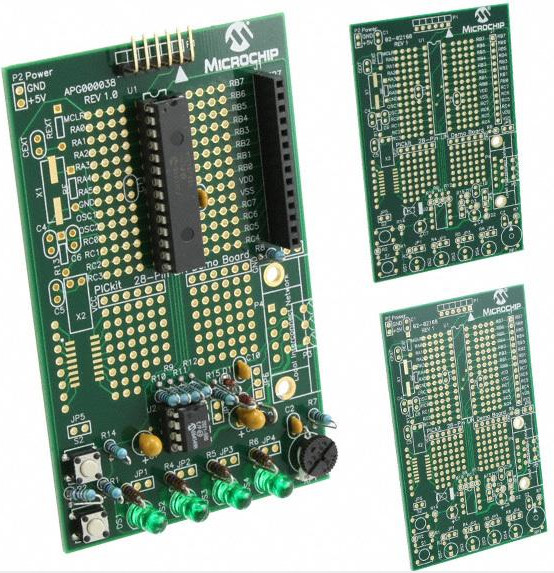
\includegraphics[width=0.95\textwidth]{./07-images/img-Ch3App/MCU-Microchip-Dev-Demo-Board.jpg}
		\caption{App3-MCU Microchip 28-Pin LIN Development Demo Interface Board}
		\label{fig:App3-MCU-Microchip-Dev-Demo-Board.jpg}
	\end{center}
\end{figure}

\subsection{App3-Specifications MCU Microchip 28-Pin LIN Development Board}

Reference: \url{https://www.digikey.my/products/en?keywords=DM164130-3-ND\%20\%20}\\
28-Pin LIN DEMO BOARD USER'S GUIDE\\
2009 Microchip Technology Inc.DSxxxxx\\
\vspace{0.5cm}

The 28-Pin LIN (Local Interconnect Network) Demo Board is a small and simple demonstration PCB for Microchip's 28-pin Dual Inline Package (DIP) PIC Microcontroller Units (MCU). It is populated with a PIC16F886 MCU, a MCP2021 LIN Transceiver with voltage regulator, four LEDs, 2 push buttons and a potentiometer. The demo board has several test points to access the I/O pins of the MCU and a generous prototyping area. The MCU can be programmed with the PICkit 2 Microcontroller Programmer or the MPLAB ICD 2 using the RJ-11 to 6-pin inline adapter (AC164110).
\vspace{0.5cm}

LIN (Local Interconnect Network) is an automotive networking technology, a sub-bus system based on a serial communications protocol. The bus is a single master/multiple slave bus that uses a single wire to transmit data.
\vspace{0.5cm}

The 28-Pin LIN Demo Board can be used with virtually any 28-pin Dual Inline Package (DIP) PIC MCU. The assembled 28-Pin LIN Demo Board is populated with a PIC16F886-I/P microcontroller. Additional 28-Pin LIN Demo Boards can be ordered from Microchip technology and distributors. Part number, DM164120-3, comes with one assembled and two blank 28-Pin LIN Demo Boards. 
\vspace{0.5cm}

The blank demo board can be used for evaluating or prototyping circuits using any of the 28-pin devices listed below.

\begin{figure}[htbp]
	\begin{center}
		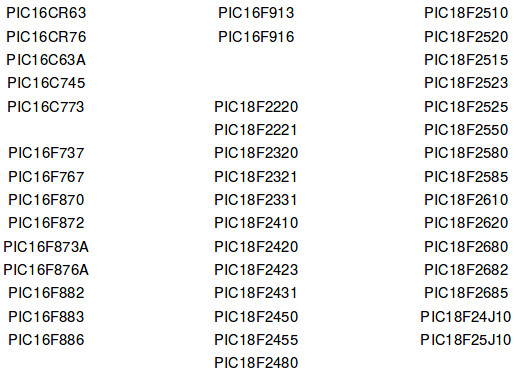
\includegraphics[width=0.85\textwidth]{./07-images/img-Ch3App/MCU-Chips-Supported-for-Dev-Demo-Board.jpg}
		\caption{App3-MCU Chips Supported-for Dev Demo Interface Board}
		\label{fig:App3-MCU-Chips-Supported-for-Dev-Demo-Board.jpg}
	\end{center}
\end{figure}

The 28-Pin LIN Demo Board is populated with a PIC16F886 MCU (U1), a MCP2021 LIN Transceiver with Voltage Regulator (U2), four LEDs (DS1-DS4), Two push buttons (SW1 and SW2), 32 KHz crystal (X2) and potentiometer (RP1). The board layout is shown in the figure below. The demo board has several test points to access the I/O pins of the MCU and a generous prototyping area. The MCU can be programmed with the PICkit 2 Microcontroller Programmer from header P1.
\vspace{0.5cm}

\pagebreak
\begin{figure}[htbp]
	\begin{center}
		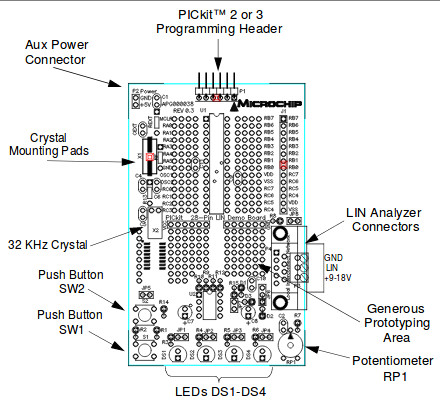
\includegraphics[width=0.95\textwidth]{./07-images/img-Ch3App/MCU-Microchip-28-Pin-LIN-Dev-Demo-Board.jpg}
		\caption{App3-MCU Microchip 28-Pin LIN Dev Demo Board Layout Diagram}
		\label{fig:App3-MCU-Microchip-28-Pin-LIN-Dev-Demo-Board.jpg}
	\end{center}
\end{figure}



% ==========================================================
\pagebreak
\subsection{App3-MCU Microchip Curiosity Development Board}\label{sec:C-3.5-Curiosity-Development-Board}

\begin{figure}[htbp]
	\begin{center}
		\includegraphics[width=0.85\textwidth]{./07-images/img-Ch3App/MCU-Curiosity-Dev-Board-Layout.jpg}
		\caption{App3-MCU Microchip Curiosity Demo Board Layout Diagram}
		\label{fig:App3-MCU-Curiosity-Dev-Board-Layout.jpg}
	\end{center}
\end{figure}
\begin{figure}[htbp]
	\begin{center}
		\includegraphics[width=0.65\textwidth]{./07-images/img-Ch3App/MCU-Curiosity-Dev-Board-Layout-Legend.jpg}
		\caption{App3-MCU Microchip Curiosity Demo Board Layout Legend}
		\label{fig:App3-MCU-Curiosity-Dev-Board-Layout-Legend.jpg}
	\end{center}
\end{figure}

\pagebreak
\subsection{App3-Specifications MCU Microchip Curiosity Development Board}
Reference: Curiosity Development Board User's Guide\\
2015-2016 Microchip Technology Inc. DS40001804B\\
\vspace{0.5cm}

The Curiosity Development Board supports Microchip's 8-pin, 14-pin and 20-pin 8-bit PIC MCUs. Dual-row expansion headers on either side of the socket offer flexibility of connectivity to all pins on the PIC MCUs. This board provides flexibility for 
experimentation through an application header with ground (GND) and supply voltage (VDD) connections. It also includes
a set of indication LEDs, mTouch button and push-button switches, and a variable potentiometer. Additionally, it features a 
Bluetooth low-energy footprint and a mikroBUS footprint to accommodate a variety of plug-in Click Board sensors that can be used in application development.
\vspace{0.5cm}

The Curiosity Development Board can be powered in one of three ways, depending on its usage.
\vspace{0.5cm}

\textbf{Power1 via USB Connector (J2)}\\

The USB connector (J2) will power the entire Curiosity Development Board. A shunt jumper must be placed onto jumper J12. The right two pins of J12 will connect +5V from the USB connector J2. The left two pins of J12 will connect +3.3V from the USB voltage regulator on the back side of the development board. With USB power connected to J2, power LED D1 will always be ON to indicate that +3.3V is available on the board. 
\vspace{0.5cm}

\textbf{Power2 via 9V External Power Supply (J15)}\\
%\vspace{0.5cm}

The 9V external power supply (J15) will also power the entire Curiosity Development Board. A shunt jumper must be placed onto jumper J12. The right two pins of J12 will connect +5V from the on-board voltage regulator circuitry connected to connector J15. The left two pins of J12 will connect +3.3V from the on-board voltage regulator circuitry. With 9V external power connected to J15, power LED D1 will always be ON to indicate that +3.3V is available on the board. Power LED D2 will only be ON when power (+3.3V or +5V) is applied to VDD via a shunt jumper placed on J12.
\vspace{0.5cm}

\textbf{Power3 via Variable External Power Supply (TP3, TP4)}\\
%\vspace{0.5cm}

A variable external power supply connected to TP3 and TP4 will power the entire Curiosity Development Board. A shunt jumper is not needed on J12, thus either +3.3V or +5V can be directly applied via a variable external power supply to VDD.
\vspace{0.5cm}


\textbf{Getting Started on Curiosity Board}\\
%\vspace{0.5cm}

The Curiosity Development Board must be used with MPLAB X Integrated Development Environment (IDE), available free on Microchip's web site, www.microchip.com. Use version v3.05 or later. The Curiosity Development Board, through MPLAB X, is a low-voltage in-circuit debugger, as well as a low-voltage programmer, for all supported devices. In-circuit debugging allows the user to run, examine and modify programs for the supported device embedded in the Curiosity hardware. This facilitates
the debugging of firmware and hardware concurrently. Use the Curiosity Development Board with MPLAB X IDE to run, stop and single-step through programs breakpoints can be set and the processor can be reset. When the processor stops, the contents of the register are available for examination and modification.
\vspace{0.5cm}

\textbf{Programming the Curiosity Board}\\
%\vspace{0.5cm}

After connecting the Curiosity Development Board to the computer using the on-board USB connector (J2 on the back of the board), open the MPLAB X IDE. Then create a new project or open an existing project. Click on the Project Properties icon located in the project's Dashboard window.
\vspace{0.5cm}

Alternatively, the Project Properties window can be opened by clicking on File, Project Properties, or by right-clicking on 
the project name in the Projects window and clicking Properties.
\vspace{0.5cm}

And it goes on.

% ==========================================================
 %% Research Methodology
% ==========================================================
\clearpage
\pagebreak
\justifying
\renewcommand{\thesection}{D \arabic{section}}

\titleformat{\section}{\normalfont\LARGE\bfseries\color{black}}{\thesection}{10pt}{\LARGE}
\section{Appendix-D4 Related Research Work}\label{sec:App4-Related-Research-Work}

%% PORTRAIT
%\pagebreak
%\clearpage
% ==========================================================
\clearpage
\pagebreak
\section{Some Results on Previous Projects}

Bismillah



%% PORTRAIT
\pagebreak
\clearpage
% ==========================================================
\clearpage
\pagebreak
%% \section{Images of Devices for Previous Projects}

\subsection{App4-Parallel Port Devices}. 
				
		\begin{figure}[htbp]
			\begin{center}
				\includegraphics[width=0.700\textwidth]{./07-images/img-Ch4/Captured-Parallel-Port-Built-in-Motherboard.jpg}
				\caption{App4-Parallel Port device built-in on Motherboard (purple)}
				\label{fig:App4-Captured-Parallel-Port-Built-in-Motherboard.jpg}
			\end{center}
		 \end{figure}
		 
		
		\begin{figure}[htbp]
			\begin{center}
\frame{\includegraphics[width=0.65\textwidth]{./07-images/img-Ch4/Captured-Parallel-Port-PCI-Adapter-Card.jpg}}
				\caption{App4-Parallel Port PCI Adapter Card}
				\label{fig:App4-Captured-Parallel-Port-PCI-Adapter-Card.jpg}
			\end{center}
		\end{figure}
The Netmos Nm9805 is a IEEE 1284 parallel port controller with PCI bus interface. Nm9805 fully supports the existing Centronics printer interface as well as PS/2, EPP, and ECP modes. Single 5V operation. Low power. PCI compatible 1284 printer port. Multi-mode compatible controller (SPP, PS2, EPP, ECP). Fast data rates up to 1.5 Mbytes/s (parallel port). Microsoft and Linux compatible. 

% ==================
\clearpage
\pagebreak
		\begin{figure}[htbp]
			\begin{center}
\frame{\includegraphics[width=0.65\textwidth]{./07-images/img-Ch4/Captured-USB-to-Parallel-Port-PL2305-Converter.jpg}}
				\caption{App4-USB to Parallel Port PL2305 Converter Cable}
				\label{fig:App4-Captured-USB-to-Parallel-Port-PL2305-Converter.jpg}
			\end{center}
		\end{figure}

		\begin{figure}[htbp]
			\begin{center}
\frame{\includegraphics[width=0.75\textwidth]{./07-images/img-Ch4/USB-to-Serial-Parallel-Idle-and-Writing-Modes.jpg}}
				\caption{App4-USB to-Serial and to-Parallel Idle(Left) and Writing(Right) Modes}
				\label{fig:App4-USB-to-Serial-Parallel-Idle-and Writing-Modes.jpg}
			\end{center}
		\end{figure}
		
LEFT PICTURE: The blue color LED status is for cable device idle and ready.\\
RIGHT PICTURE: The red color LED status is for cable device busy during active reading and writing modes.  
	
\lstset{basicstyle=\ttfamily\small}
%% \lstset{basicstyle=\ttfamily\tiny}
\begin{lstlisting}[breaklines, frame=single, caption={App4-Detection of USB-to-Parallel Cable}, label=App4-usb-to-paralle-PL2305-cable-detected]
Bus 001 Device 021: ID 067b:2305 Prolific Technology, Inc. 
PL2305 Parallel Port  <=== FOUND 
[ 3978.848284] usb 1-1.6: Manufacturer: Prolific Technology Inc.
[ 3978.855271] usblp 1-1.6:1.0: usblp0: USB Bidirectional 
printer dev 21 if 0 alt 1 proto 2 vid 0x067B pid 0x2305
\end{lstlisting}

		
% ==================
\clearpage
\pagebreak
		
\subsection{App4-Velleman K8000 Parallel Interface Board}

	\begin{figure}[htbp]
		\begin{center}
\frame{\includegraphics[width=0.85\textwidth]{./07-images/img-Ch4/Captured-Velleman-K8000-Parallel-Port-Extension-Board.jpg}}
			\caption{App4-Velleman K8000 Parallel Port Extension Board}
			\label{fig:App4-Captured-Velleman-K8000 Parallel-Port-Extension-Board.jpg}
		\end{center}
	\end{figure}
	
\lstset{basicstyle=\ttfamily\small}
%% \lstset{basicstyle=\ttfamily\tiny}
\begin{lstlisting}[breaklines, frame=single, caption={App4-Specifications of Velleman K8000 Parallel Interface Board}, label=App4-Specifications-Velleman-K8000-Interface-Board]
DIGITAL OUTPUTS:
    optocoupler, open collector output: 50mA - max. 30VDC
DIGITAL INPUTS:
    optocoupler input: 5V/5mA, max. 20V/40mA
ANALOG OUTPUTS:
    8 outputs DAC1 to DAC8, resolution: 64 steps
    minimum output voltage: 0.1V at 2mA
    maximum output voltage: 11.5V adjustable at 2mA
    resolution per step from 0.1 to 11.5V: 160mV +/- 90mV
    1 precision output DA1, resolution: 256 steps
    minimum output voltage: 0V
    maximum output voltage: 4.5V adjustable at 0.5mA
    resolution per step from 0 to 4.5V: 17.5mV
ANALOG INPUTS:
    4 analogue inputs AD1 to AD4, resolution: 256 steps
    minimum input voltage: 0V
    maximum input voltage: 5V
    input impedance: 50Mohm
    resolution: 19.5mV
    communication protocol: I2Cbus
    LED indication for each I/O
BOARD:
    25 pin D series connector for computer
    25 pin D series connector for printer
    supply voltage: 230Vac
    PCB dimensions: 237 x 133mm (9.3" x 5.2")
\end{lstlisting}			
			
%================================================		
\clearpage
\pagebreak		
		
\subsection{App4-Velleman K8055 USB Interface Board}
	
\begin{figure}[htbp]
	\begin{center}
\frame{\includegraphics[width=0.85\textwidth]{./07-images/img-Ch4/Captured-Velleman-K8055-USB-Extension-Board.jpg}}
\caption{App4-Velleman K8055 USB Port Extension Board}
\label{fig:App4-Captured-Velleman-K8055-USB-Extension-Board.jpg}
	\end{center}
\end{figure}

\lstset{basicstyle=\ttfamily\small}
%% \lstset{basicstyle=\ttfamily\tiny}
\begin{lstlisting}[breaklines, frame=single, caption={App4-Specifications of Velleman K8055 USB Interface Board}, label=App4-Specifications-Velleman-K8055-USB-Interface-Board]
DIGITAL INPUTS:
    5 digital inputs (0 = ground, 1 = open) 
    (on board test buttons provided)
ANALOG INPUTS:
    2 analogue inputs with attenuation and amplification 
    option (internal test +5V provided)
DIGITAL OUTPUTS:
    8 digital open collector output switches 
    (max. 50V/100mA) (on board LED indication)
ANALOG OUTPUTS:
    2 analogue outputs:
    0 to 5V, output resistance 1K5
    PWM 0 to 100% open collector outputs 
    max 100mA / 40V (on board LED indication)
    general conversion time: 20ms per command
BOARD:    
    power supply through USB: approx. 70mA
    dimensions: 145 x 88 x 20mm / 5.7 x 3 x 0.8"
\end{lstlisting}


%================================================		
\clearpage
\pagebreak

\subsection{App4-Heber X10i USB Board}.

\begin{figure}[htbp]
	\begin{center}
		\frame{\includegraphics[width=0.85\textwidth]{./07-images/img-Ch4/Captured-Heber-X10i-USB-Extension-Board.jpg}}
		\caption{App4-Heber X10i USB Port Extension Board}
		\label{fig:App4-Captured-Heber-X10i-USB-Extension-Board.jpg}
	\end{center}
\end{figure}


\lstset{basicstyle=\ttfamily\small}
%% \lstset{basicstyle=\ttfamily\tiny}
\begin{lstlisting}[breaklines, frame=single, caption={App4-Specifications of Heber-X10i USB Interface Board}, label=App4-Specifications-Heber-X10i-USB-Interface-Board]
Heber X10i = USB real-time PC I/O controller
HARDWARE:
	64 Switched Inputs / Outputs
	Real-time I/O processor
	Battery backed SRAM
	Secure data retention
	DALLAS unique identifier
	Audio amp 5W RMS, Stereo audio amplifier
	Serial I/O
	SEC meter
	ccTalk
	LED control
	EEPROM 32KB
	Real time clock
	Current sensing 12v supply
	Open drain outputs for lamps and meters
	High current outputs
SOFTWARE:
	Serial I/O: RS232, TTL, ccTalk
	On-board security device
	Program in C, C+, C# or BlitzMax
	Microsoft Windows XPe / Linux / Raspberry Pi drivers
\end{lstlisting}

%================================================		
\clearpage
\pagebreak		
		
\subsection{App4-Arduino Due USB Board}. 

\begin{figure}[htbp]
	\begin{center}
		\frame{\includegraphics[width=0.85\textwidth]{./07-images/img-Ch4/Captured-Arduino-Due-USB-Extension-Board.jpg}}
		\caption{App4-Arduino Due USB Port Extension Board}
		\label{fig:App4-Captured-Arduino-Due-USB-Extension-Board.jpg}
	\end{center}
\end{figure}

Unlike most Arduino boards, the Arduino Due board runs at 3.3V. The maximum voltage that the I/O pins can tolerate is 3.3V. Applying voltages higher than 3.3V to any I/O pin could damage the board. 
\vspace*{1\baselineskip}

The SAM3X provides one hardware UART and three hardware USARTs for TTL (3.3V) serial communication.

\lstset{basicstyle=\ttfamily\small}
%% \lstset{basicstyle=\ttfamily\tiny}
\begin{lstlisting}[breaklines, frame=single, caption={App4-Specifications of Arduino Due USB Interface Board}, label=App4-Specifications-Arduino-Due-USB-Interface-Board]
Microcontroller 	AT91SAM3X8E
Operating Voltage 	3.3V
Input Voltage (recommended) 7-12V
Input Voltage (limits) 	6-16V
Digital I/O Pins 	54 (of which 12 provide PWM output)
Analog Input Pins 	12
Analog Output Pins 	2 (DAC)
Total DC Output Current on all I/O lines 	130 mA
DC Current for 3.3V Pin 	800 mA
DC Current for 5V Pin 	800 mA
Flash Memory 	512 KB all available for the user applications
SRAM 	96 KB (two banks: 64KB and 32KB)
Clock Speed 	84 MHz
Length 	101.52 mm
Width 	53.3 mm
Weight 	36 g
\end{lstlisting}

%================================================		
\clearpage
\pagebreak
		
\subsection{App4-Nexys-3 Spartan-6 FPGA USB Board}. 


\begin{figure}[htbp]
	\begin{center}
\frame{\includegraphics[width=0.80\textwidth]{./07-images/img-Ch4/Captured-Nexys3-Spartan6-FPGA-USB-Extension-Board.jpg}}
		\caption{App4-Nexys-3 Spartan-6 FPGA USB Port Extension Board}
		\label{fig:App4-Captured-Nexys3-Spartan6-FPGA-USB-Extension-Board.jpg}
	\end{center}
\end{figure}

Nexys 3 is compatible with all Xilinx CAD tools, including ChipScope, EDK, and the free WebPack. The Nexys 3 uses Digilent's newest Adept USB2 system that offers FPGA and ROM programming, automated board tests, virtual I/O, and simplified user data transfer facilities. In our project we used the Adept USB2 system.

\lstset{basicstyle=\ttfamily\small}
%% \lstset{basicstyle=\ttfamily\tiny}
\begin{lstlisting}[breaklines, frame=single, caption={App4-Specifications of Nexys-3 Spartan-6 FPGA USB Interface Board}, label=App4-Specifications-Nexys-3-Spartan-6-FPGA-USB-Interface-Board]
Xilinx Spartan-6 LX16 FPGA in a 324 pin BGA package
16 Mbyte Cellular RAM (x16)
16Mbytes SPI (quad mode) PCM non volatile memory
16Mbytes parallel PCM non volatile memory
10/100 Ethernet PHY
On board USB2 port for programming and data xfer
USB UART and USB
HID port (for mouse/keyboard)
8 bit VGA port
100 MHz CMOS oscillator
72 I/Os routed to expansion connectors
GPIO includes 8 LEDs, 5 buttons, 8 slide switches and 
4-digit seven segment display
USB v2 - programming cable included
\end{lstlisting}


%================================================		
\clearpage
\pagebreak

\subsection{App4-Raspberry Pi-3 Model-B Single Board Computer}. 

\begin{figure}[htbp]
	\begin{center}
		\frame{\includegraphics[width=0.85\textwidth]{./07-images/img-Ch4/Captured-Raspberry-Pi3-ModelB-SBC.jpg}}
		\caption{App4-Raspberry Pi-3 Model-B Single Board Computer}
		\label{fig:App4-Captured-Raspberry-Pi3-ModelB-SBC.jpg}
	\end{center}
\end{figure}

\subsection{App4-Raspberry Pi-2 Model-B Single Board Computer}.

\begin{figure}[htbp]
	\begin{center}
		\frame{\includegraphics[width=0.85\textwidth]{./07-images/img-Ch4/Captured-Raspberry-Pi2-ModelB-SBC.jpg}}
		\caption{App4-Raspberry Pi-2 Model-B Single Board Computer}
		\label{fig:App4-Captured-Raspberry-Pi2-ModelB-SBC.jpg}
	\end{center}
\end{figure}

%================================================		
\clearpage
\pagebreak

\lstset{basicstyle=\ttfamily\small}
%% \lstset{basicstyle=\ttfamily\tiny}
\begin{lstlisting}[breaklines, frame=single, caption={App4-Specifications of Raspberry Pi 3 SBC Board}, label=App4-Specifications-of -Raspberry-Pi-3-SBC-Board]
SoC: Broadcom BCM2837
CPU: 4 x ARM Cortex-A53, 1.2GHz
GPU: Broadcom VideoCore IV
RAM: 1GB LPDDR2 (900 MHz)
Networking: 10/100 Ethernet, 2.4GHz 802.11n wireless
Bluetooth: Bluetooth 4.1 Classic, Bluetooth Low Energy
Storage: microSD
GPIO: 40-pin header, populated
Ports: HDMI, 3.5mm analogue audio-video jack, 
4 x USB 2.0, Ethernet, Camera Serial Interface (CSI), 
Display Serial Interface (DSI)
And more ....
\end{lstlisting}

\lstset{basicstyle=\ttfamily\small}
%% \lstset{basicstyle=\ttfamily\tiny}
\begin{lstlisting}[breaklines, frame=single, caption={App4-Specifications of Raspberry Pi 2 SBC Board}, label=App4-Specifications-of -Raspberry-Pi-2-SBC-Board]
SoC: Broadcom BCM2836 (CPU, GPU, DSP, SDRAM)
CPU: 900 MHz quad-core ARM Cortex A7 (ARMv7 instruction set)
GPU: Broadcom VideoCore IV @ 250 MHz
More GPU info: OpenGL ES 2.0 (24 GFLOPS); 1080p30 MPEG-2 
and VC-1 decoder (with license), h.264/MPEG-4 AVC 
high-profile decoder and encoder
Memory: 1 GB (shared with GPU)
USB ports: 4
Video input: 15-pin MIPI camera interface (CSI) connector
Video outputs: HDMI, composite video (PAL and NTSC)
via 3.5 mm jack
Audio input: I2S
Audio outputs: Analog via 3.5 mm jack; digital 
via HDMI and I2S
Storage: MicroSD
Network: 10/100Mbps Ethernet
Peripherals: 17 GPIO plus specific functions, and HAT ID bus
Power rating: 800 mA (4.0 W)
Power source: 5 V via MicroUSB or GPIO header
Size: 85.60mm x 56.5mm
Weight: 45g (1.6 oz)
\end{lstlisting}


%================================================		
\clearpage
\pagebreak

\subsection{App4-Banana Pi M2U Single Board Computer}.

\begin{figure}[htbp]
	\begin{center}
		\frame{\includegraphics[width=0.85\textwidth]{./07-images/img-Ch4/Banana-PI-M2U-SBC.jpg}}
		\caption{App4-Banana Pi M2U Single Board Computer}
		\label{fig:App4-Banana-PI-M2U-SBC.jpg}
	\end{center}
\end{figure}

\lstset{basicstyle=\ttfamily\small}
%% \lstset{basicstyle=\ttfamily\tiny}
\begin{lstlisting}[breaklines, frame=single, caption={App4-Specifications of Banana Pi M2U SBC Board}, label=App4-Specifications-of -Banana-Pi-M2U-SBC-Board]
Soc 	Allwinner R40/V40
CPU 	quad-core cortex-A7,the most power efficient CPU core 
GPU 	dual-core MALI-400 MP2 and runs at 500MHz, 
GPU provides OpenGL ES 2.0, hardware-accelerated OpenVG, 
1080p45 H.264 high-profile encode and decode.
SDRAM 	2 GB DDR3 with 733MHz\(shared with GPU\)
SATA 	suppoort SATA interface
GPIO 40 Pins Header, 28 x GPIO, for UART, I2C, SPI, PWM, I2S.
On board Network 10/100/1000Mbps Ethernet\(Realtek RTL8211E)
Wifi Module 	WiFi 802.11 b/g/n \(AP 6212 module on board\)
Bluetooth 	BT4.0, Storage MicroSD\(TF\) card, 8GB eMMC 
Display 4-lane MIPI DSI display,or RGB panel, LVDS panel,
Video 	Multi-format FHD video decoding, including Mpeg1/2, 
Mpeg4, H.263, H.264, etc H.264 decode up to 1080P60,support 
Audio outputs 	HDMI, analog audio \(via 3.5 mm TRRS jack\)
Camera 	A CSI input connector Camera:Supports 8-bit YUV422 
CMOS sensor interface,Supports CCIR656 protocol for NTSC, PAL,
Supports 5M pixel camera sensor,Supports video capture 
solution up to 1080p at 30fps
Audio 	input On board microphone
USB 	2 USB 2.0 host, 1 USB 2.0 OTG
Buttons Reset button, Power button, U-boot button
Leds 	Power status Led and RJ45 Led
IR	onboard IR receiver
DC Power 5V/2A with micro USB port
battery	3.7V lithium battery power support
Sizes	85mmX56mm,same size as raspberry pi 3, Weight 40g 
\end{lstlisting}

%================================================		
\clearpage
\pagebreak

\subsection{App4-Beagle-Board xM Single Board Computer}.

\begin{figure}[htbp]
	\begin{center}
		\frame{\includegraphics[width=0.85\textwidth]{./07-images/img-Ch4/Beagle-Board-xM-SBC.jpg}}
		\caption{App4-Beagle-Board xM Single Board Computer}
		\label{fig:App4-Beagle-Board-xM-SBC.jpg}
	\end{center}
\end{figure}

\lstset{basicstyle=\ttfamily\small}
%% \lstset{basicstyle=\ttfamily\tiny}
\begin{lstlisting}[breaklines, frame=single, caption={App4-Specifications of Beagle Board xM SBC Board}, label=App4-Specifications-of-Beagle-Board-xM-SBC-Board]
    Processor TI DM3730 Processor 1 GHz ARM Cortex-A8 core
    HD capable TMS320C64x+ core (800 MHz - 720p 30 fps)
    Imagination Technologies PowerVR SGX 2D/3D 
    graphics processor supporting dual independent displays
    512 MB LPDDR RAM, MicroSD/MMC card
    4 GB microSD card supplied with the BeagleBoard-xM 
    and loaded with The Angstrom Distribution
    DVI-D (HDMI connector chosen for size - maximum 
    resolution is 1400x1050)  S-Video
    USB OTG (mini AB), 4 USB ports, Ethernet
    Stereo in and out jacks
    RS-232 port  JTAG connector
    Power socket (5 V barrel connector type)
    Camera port, Expansion port
    Boot code stored on the uSD card, Boot from uSD/MMC only
    Alternative Boot source button.
    Has been demonstrated using Android,[18] 
    Angstrom Linux,[19] Fedora, Ubuntu, Gentoo,
    Arch Linux ARM and Maemo Linux distributions,
    FreeBSD, the Windows CE operating system, and RISC OS.
\end{lstlisting}

%% ===============================================

\begin{flushleft}
\begin{landscape}
%% BEGIN LANDSCAPE ENTIRELY
\pagebreak
\clearpage
%===========================================================
%%% LANDSCAPE BEGINS =======================================
%% \pagebreak
%% \clearpage
%%\begin{flushleft}
%%\begin{landscape}
	
% =========================================================
\subsection{App4-Summary main() function C-Code listing for RTAI}

% ==========================================================
\lstset{basicstyle=\footnotesize, numberstyle=\tiny\color{blue}, frame=single, numbers=left, firstnumber=1, stepnumber=1, numbersep=1pt, xleftmargin=2.0em, framexleftmargin=1.5em, xrightmargin=0.0em, breaklines=true, breakatwhitespace=false, breakindent=5pt, prebreak=\space, postbreak=\space }
% ==========================================================

\begin{lstlisting}[caption={App4-Summary main() function C-Code listing for RTAI}, label=App4-Summary main() function C-Code listing for RTAI]

// File: rtai-CNC14.c
// Date: May 05, 2018 10:04
// Author: WRY
// =========================================================
int main(int argc, char* argv[]) {
// =========================================================
WRY00_Print_DateTime_Usec(); 
printf("Bismillah from WRY executed in main().\n\n");
	
// FOR KEYBOARD INTERRUPT TO STOP (e.g. <Ctrl-C>) EXECUTION
	signal(SIGTERM, WRYcleanup);
	signal(SIGINT,  WRYcleanup);
	signal(SIGKILL, WRYcleanup);
// INVOKE FUNCTIONS SEQUENTIALLY TO RUN RTAI
	system("./load-rtai-modules.sh"); // LOAD RTAI KERNEL MODULES
	WRY01_Create_and_Initialize_Real_Time_Task_LXRT();
	WRY02_Get_Address_and_Name_of_Real_Time_Task_LXRT();
	WRY31_Make_Hard_Real_Timer_Run(); 
	WRY32_Check_Selected_Hard_Real_Time_Run_Mode(); 
	WRY33_Execute_Selected_Hard_Real_Time_Run_Mode();
	WRY04_Allow_NonRoot_Users_For_Hard_Real_Time();
	WRY05_Lock_Memory_Swapping_For_Hard_Real_Time();
	WRY06_ParallelPort_Request_StartUp_and_Enable_IRQ(); 
	WRY07_ParallelPort_Check_RT_Task_Running_Mode();
	WRY08_Start_Run_CNC_Machine();
	WRY09_Stop_Run_CNC_Machine();
	system("./unload-rtai-modules.sh"); // UNLOAD RTAI KERNEL MODULES

WRY00_Print_DateTime_Usec(); 
printf("Alhamdulillah from WRY executed in main().\n"); 
return (0);
}
\end{lstlisting}

\pagebreak
%% =========================================================
\subsection{App4-Full C-Code listing for Real Time (RTAI)}
% ==========================================================
\lstset{basicstyle=\footnotesize, numberstyle=\tiny\color{blue}, frame=single, numbers=left, firstnumber=1, stepnumber=1, numbersep=1pt, xleftmargin=2.0em, framexleftmargin=1.5em, xrightmargin=0.0em, breaklines=true, breakatwhitespace=false, breakindent=5pt, prebreak=\space, postbreak=\space }
% ==========================================================
%% \begin{lstlisting}[caption={Putting listing codes in landscape format}, label=how-to-display-in-landscape]
\begin{lstlisting}[caption={App4-Full C-Code listing for Real Time (RTAI)}, label=App4-Full C-Code listing for Real Time (RTAI)]
// File: rtai-CNC14.c
// Date: May 05, 2018 10:04
// Author: WRY
// 
// =========================================================
// (1) The prefixes WRY and TASK were used extensively in
// order to differentiate our own defined variables and functions 
// from standard C/C++ and RTAI libraries defined variables and functions.
// 
// (2) We must either link our C/C++ program against liblxrt or we 
// have to configure RTAI with "CONFIG_RTAI_LXRT_STATIC_INLINE=y".
// during linux kernel compilation.
//
// =========================================================
// STANDARD C/C++ HEADER FILES USED
// ========================================================= 

	#include <sched.h>	// Scheduler
	#include <stdio.h>	// Standard Input/Output 
	#include <stdlib.h> 	// Standard Library
	#include <time.h>	// For local date-time with usec
	#include <signal.h> 	// Signal for user interrupts, <Ctrl>-C to stop 
	#include <fcntl.h>  	// For file control
	#include <math.h>	// Mathematical functions
	#include <unistd.h> 	// Low level constants, types, function declarations
	#include <errno.h>	// Printing C errors
	#include <string.h>	// Handling strlen IN gcode . h
	#include <curses.h>	// Handling getch () , wgetch ()
	#include <sys/ioctl.h>	// System Input/Output control
	#include <sys/io.h>	// System Input/Output
	#include <sys/mman.h>	// System Memory Manager
	#include <sys/time.h>	// For system local date-time with usec




// ========================================================
// REALTIME HEADER FILES (RTAI)
// ========================================================
	#include <rtai.h>		// RTAI configuration switches (User space and Kernel space)
	#include <rtai_lxrt.h>  	// RTAI User Space libraries

// =========================================================
// RTAI VER. 5.1 DOCUMENTATION REFERENCES
// =========================================================
/*
	For full RTAI Ver 5.1 LOCAL DOCUMENTATION
		file:///usr/realtime/share/doc/rtai-5.1/html/api/files.html
	For <rtai.h>
		file:///usr/realtime/share/doc/rtai-5.1/html/api/rtai_8h_source.html
	For <rtai_lxrt.h>
		file:///usr/realtime/share/doc/rtai-5.1/html/api/rtai__lxrt_8h.html
	For <rtai_sem.h>
		file:///usr/realtime/share/doc/rtai-5.1/html/api/rtai__sem_8h.html
	For <rtai_sched.h>
		file:///usr/realtime/share/doc/rtai-5.1/html/api/rtai__sched_8h_source.html
	For <rtai_usi.h>
		file:///usr/realtime/share/doc/rtai-5.1/html/api/rtai__usi_8h_source.html
*/
// =========================================================
// EXAMPLE USAGE OF RTAI FUNCTIONS (INTERRUPT-BASED)
// ========================================================= 
/*	rt_set_oneshot_mode();
	rt_set_periodic_mode();
	start_rt_timer();
	rt_request_irq_task(PARPORT_IRQ, WRY_RT_task, RT_IRQ_TASK, 1)
	rt_task_init(); 
	rt_task_make_periodic(); 
	rt_make_hard_real_time();
	rt_make_soft_real_time();
	rt_allow_nonroot_hrt();
	rt_task_delete(WRY_RT_task);
	stop_rt_timer();
*/

// ========================================================-
// RTAI DEFINED FUNCTIONS
// =========================================================
/*
	static void * 		rt_get_adr (unsigned long name);
		Get an object address by its name. 
		Returns the address associated to name on success, 0 on failure 
	
	static unsigned long 	rt_get_name (void *adr);
		Get an object name by its address. 
		Returns the address associated to name on success, 0 on failure 
	
	static RT_TASK * 	rt_task_init (unsigned long name, int priority, int stack_size, int max_msg_size);
		Create an RTAI task extension for a Linux process/task in user space.
	
	static void 		rt_make_soft_real_time (void);
		Return a hard real time Linux process, or pthread to the standard Linux behavior.
	
	static void 		rt_make_hard_real_time (void);
		Give a Linux process, or pthread, hard real time execution capabilities allowing full kernel preemption
	
	static void 	rt_allow_nonroot_hrt (void);
		Allows a non root user to use the Linux POSIX soft real time process management and memory lock functions, and allows it to do any input-output operation from user space.
*/
// ========================================================
// GLOBAL DEFINITIONS
// ========================================================
	#define PERIOD		500000		// nanoseconds
	#define TICK_TIME	1000000		// nanoseconds
	// #define CPUMAP 	0xF  		// 16-cpus
	#define CPUMAP		0x4		// 4-cpus
	
	// BUILT_IN PARALLEL PORT ON MOTHERBOARD
	// #define PARPORT_IRQ	7
	// #define BASEPORT	0x378
	
	// HARDWARE 1 = parport0: PC-style at 0xd010 (0xd000), irq 18
	#define BASEPORT	0xd010
	#define PARPORT_IRQ	18

	// HARDWARE 2 = parport1: PC-style at 0xe100, irq 17
	// #define BASEPORT	0xe100
	// #define PARPORT_IRQ	17

	static volatile int ovr, intcnt, retval, maxcnt;

// =========================================================
// HARDWARE DEVICES PARALLEL PORT SEARCH
// =========================================================
/* EXECUTE SYSTEM FUNCTION
root@dell-ub1604-64b:/home/wruslan# dmesg | grep parp

KERNEL MESSAGE - FOUND PARALLEL PORT NO. 1
	[    8.989048] parport0: PC-style at 0xd010 (0xd000), irq 18, using FIFO [PCSPP,TRISTATE,COMPAT,EPP,ECP]
	[    9.089563] lp0: using parport0 (interrupt-driven).
	
KERNEL MESSAGE - FOUND PARALLEL PORT NO. 2
	[   11.972056] parport1: PC-style at 0xe100, irq 17 [PCSPP,TRISTATE]
	[   12.073309] lp1: using parport1 (interrupt-driven).

root@dell-ub1604-64b:/home/wruslan# lspci -v

LIST PCI DEVICE - FOUND PARALLEL PORT NO. 1
	03:00.0 Parallel controller: Oxford Semiconductor Ltd Device c110 (prog-if 02 [ECP])
	Subsystem: Oxford Semiconductor Ltd Device c110
	Flags: bus master, fast devsel, latency 0, IRQ 18
	I/O ports at d010 [size=8]
	I/O ports at d000 [size=4]
	Capabilities: [40] Power Management version 3
	Capabilities: [50] MSI: Enable- Count=1/1 Maskable- 64bit+
	Capabilities: [70] Express Legacy Endpoint, MSI 00
	Capabilities: [100] Device Serial Number 00-30-e0-11-11-00-01-10
	Capabilities: [110] Power Budgeting <?>
	Kernel driver in use: parport_pc
	Kernel modules: parport_pc

	
LIST PCI DEVICE - FOUND PARALLEL PORT NO. 2
	02:00.0 Serial controller: Device 1c00:3250 (rev 10) (prog-if 05 [16850])
	Subsystem: Device 1c00:3250
	Flags: fast devsel, IRQ 17
	I/O ports at e000 [size=256]
	Memory at f0100000 (32-bit, prefetchable) [size=32K]
	I/O ports at e100 [size=4]
	Expansion ROM at f7c00000 [disabled] [size=32K]
	Capabilities: [60] Power Management version 3
	Capabilities: [68] MSI: Enable- Count=1/32 Maskable+ 64bit+
	Capabilities: [80] Express Legacy Endpoint, MSI 00
	Capabilities: [100] Advanced Error Reporting
	Kernel driver in use: parport_serial
	Kernel modules: parport_serial

*/
// ========================================================
// REAL TIME OBJECTS
// ========================================================
	static RT_TASK* 	WRYtask;
	static RT_TASK*     	WRY_RT_task;
	struct sched_param 	WRYsched;
	struct timeval 		WRYstart, WRYfinish;
	unsigned long 		WRY_RT_task_name; 

// ========================================================
// TIMING FOR GENERAL CNC EXECUTION
// ========================================================
	static RTIME 		CNCunixtime1, CNCunixtime2;
	static RTIME		CNCstart_time_ns, CNCcurrent_time_ns;
	static RTIME		CNCend_time_ns, CNCrun_duration_ns;
	static RTIME 		CNCtimer_period_ns; // timer period, in nanoseconds
	RTIME 			CNCtimer_period_count; //actual timer period, in counts




// ========================================================
// TIMING FOR INDIVIDUAL TASK EXECUTION
// ========================================================
	struct timeval 		TASKstart, TASKfinish;
	long int		TASKusec_duration;
	double			TASKsec_duration;

// ========================================================
// GLOBAL VARIABLES (With KEYBOARD Interrupt)
// ========================================================
	int 			WRYpriority     = 0; // Highest
	int 			WRYstack_size   = 0; // Using default (512)
	int 			WRYmax_msg_size = 0; // Using default (256)
	int 			WRYpolicy 	= SCHED_FIFO;
	int 			WRYcpus_allowed	= CPUMAP;
	long int 		WRYusec_duration;
	double 			WRYsec_duration ;
	int			WRYsig;  // Keyboard interrupt signal <Ctrl>-C
	static volatile int 	ovr, intcnt, retval, maxcnt;

// =======================================================
// DEFINE REALTIME TASK STATUS AND SETTINGS
// =======================================================
// REFERNCE: Initially task status set to non-periodic (value non-zero)
// Later on in program we make task periodic (change value to 0)

	int 		WRY_RT_task_status = 1;  
	static RTIME 	WRYexpected;
	static RTIME 	WRYsampling_interval;	

// SELECT REAL TIME TIMER PERIOD
	static RTIME 	CNCtimer_period_ns = 1000*1000*1000; // means (1 sec) period

// SET REAL TIME RUN MODE (BOTH CANNOT BE TRUE)
	int 		WRY_set_periodic_mode = 1; // TRUE  = 1 
	int		WRY_set_one_shot_mode = 0; // FALSE = 0

// SELECTED RUN MODE VALUES (PERIODIC == 1, ONE-SHOT == 2)
	int 		WRY_selected_run_mode; 

// TASK PERIODIC STATUS VALUES (PERIODIC == 0, NON-PERIODIC != 0)
	int 		WRY_task_periodic_status;

// TASK ONE-SHOT STATUS VALUES (ONE-SHOT ???, NON-ONE-SHOT ???)
	int 		WRY_task_one_shot_status;




// =======================================================
// GLOBAL DATA STRUCTURES 
// =======================================================
// Used for WRY00_Print_DateTime_Usec(void) ONLY in order 
// to avoid repetitive declarations (reused) 

	time_t 		WRYtimer;
	char 		WRYbuffer[26];
	struct tm*	WRYtm_info;
	struct timeval	WRYtval_now;




// ========================================================
void WRY00_Print_DateTime_Usec(void) {
// ========================================================
// EXECUTIONS
	time(&WRYtimer);
	WRYtm_info = localtime(&WRYtimer);
	strftime(WRYbuffer, 26, "%Y-%m-%d %H:%M:%S", WRYtm_info);
	gettimeofday(&WRYtval_now, NULL);
	printf("%s", WRYbuffer);
	printf(".%09ld \t", (long int)WRYtval_now.tv_usec);
}




// =======================================================
void WRY01_Create_and_Initialize_Real_Time_Task_LXRT(void) {
// =======================================================
WRY00_Print_DateTime_Usec(); 
printf("STARTED  WRY01_Create_and_Initialize_Real_Time_Task-LXRT(void).\n");

// Create an RTAI task extension for a Linux process/task in user space.

	if (!(WRY_RT_task = rt_task_init(nam2num("CNC06"), WRYpriority, WRYstack_size, WRYmax_msg_size))) {
		WRY00_Print_DateTime_Usec();
		printf("ERROR : Cannot initialize real time task LXRT.\n");
		WRY00_Print_DateTime_Usec();
		printf("ERROR DESCRIPTION : %s\n", strerror(errno));
		exit(1);
	} else {
		WRY00_Print_DateTime_Usec();
		printf("SUCCESS: Completed real time task LXRT initialization.\n");
	}

WRY00_Print_DateTime_Usec(); 
printf("FINISHED WRY01_Create_and_Initialize_Real_Time_Task-LXRT(void).\n\n");
}

// =======================================================
void WRY02_Get_Address_and_Name_of_Real_Time_Task_LXRT(void) {
// =======================================================
WRY00_Print_DateTime_Usec(); 
printf("STARTED  WRY02_Get_Address_and_Name_of_Real_Time_Task_LXRT(void).\n");

	// GET RT_TASK NAME BY ADDRESS
	if (rt_get_name(WRY_RT_task) == 0) {
		WRY00_Print_DateTime_Usec();
		printf("ERROR : Cannot get name of real time task LXRT.\n");
		WRY00_Print_DateTime_Usec();
		printf("ERROR DESCRIPTION : %s\n", strerror(errno));
	//	exit(1);
	} else {
		WRY00_Print_DateTime_Usec();
		printf("SUCCESS: NAME of real time task LXRT = %p\n", (void *)WRY_RT_task);
		WRY_RT_task_name = (unsigned long)WRY_RT_task;
	}

WRY00_Print_DateTime_Usec(); 
printf("FINISHED WRY02_Get_Address_and_Name_of_Real_Time_Task_LXRT(void).\n\n");
}

// ========================================================
void WRY31_Make_Hard_Real_Timer_Run(void) {
// ========================================================
WRY00_Print_DateTime_Usec(); 
printf("STARTED  WRY31_Make_Hard_Real_Timer_Run(void).\n");

	// EXECUTE HARD REAL TIMER CLOCK
	rt_make_hard_real_time();
	
	// IF HARD REAL TIME ALREADY RUNNING, NOTIFY STATUS
	if (rt_is_hard_timer_running()) {
		WRY00_Print_DateTime_Usec();
		printf("SUCCESS: Hard real timer is already running.\n");
	} else {
		// IF NOT RUNNING, START WHILE LOOP
		while (!(rt_is_hard_timer_running())) {
	
			// EXECUTE HARD REAL TIMER CLOCK
			rt_make_hard_real_time();
			// IF HARD REAL TIMER IS NOT RUNNING, THEN RUN IT BY LOOPING.
			if (rt_is_hard_timer_running()) {
				WRY00_Print_DateTime_Usec();
				printf("SUCCESS: Hard real timer is NOW running.\n");
			} else {
				WRY00_Print_DateTime_Usec();
				printf("FAILED : Hard real timer is NOT YET running.\n");
				WRY00_Print_DateTime_Usec();
				printf("ERROR DESCRIPTION : %s\n", strerror(errno));
				// exit(1); // DISABLED TO KEEP ON TRYING
			} END if else    
		} // END while loop
	} // END if else

WRY00_Print_DateTime_Usec(); 
printf("FINISHED WRY31_Make_Hard_Real_Timer_Run(void).\n\n");
}

// ========================================================
void WRY32_Check_Selected_Hard_Real_Time_Run_Mode(void) {
// ========================================================
WRY00_Print_DateTime_Usec(); 
printf("STARTED  WRY32_Check_Selected_Hard_Real_Time_Run_Mode(void).\n");

	// BOTH RUN MODES SELECTED
	if ((WRY_set_periodic_mode == 1) && (WRY_set_one_shot_mode == 1)) {
		WRY00_Print_DateTime_Usec();
		printf("ERROR : Cannot select both periodic_mode and one-shot mode.\n");
		exit(1); 	
		} 
	// NO RUN MODE SELECTED
	if ((WRY_set_periodic_mode == 0) && (WRY_set_one_shot_mode == 0)) {
		WRY00_Print_DateTime_Usec();
		printf("ERROR : No hard realtime run mode selected.\n");
		exit(1); 	
		} 
	// PERIODIC MODE SELECTED
	if ((WRY_set_periodic_mode == 1) && (WRY_set_one_shot_mode == 0)) {
		WRY00_Print_DateTime_Usec();
		printf("SUCCESS: PERIODIC hard realtime run mode selected.\n");
		WRY_selected_run_mode = 1; 	
		} 
	// ONE-SHOT MODE SELECTED
	if ((WRY_set_periodic_mode == 0) && (WRY_set_one_shot_mode == 1)) {
		WRY00_Print_DateTime_Usec();
		printf("SUCCESS: ONE-SHOT hard realtime run mode selected.\n");
		WRY_selected_run_mode = 2;	
		}
WRY00_Print_DateTime_Usec(); 
printf("FINISHED WRY32_Check_Selected_Hard_Real_Time_Run_Mode(void).\n\n");
}

// ========================================================
void WRY33_Execute_Selected_Hard_Real_Time_Run_Mode(void) {
// ========================================================
WRY00_Print_DateTime_Usec(); 
printf("STARTED  WRY33_Execute_Selected_Hard_Real_Time_Run_Mode(void).\n");

	// FOR PERIODIC-MODE REAL TIME RUN
	if (WRY_selected_run_mode == 1) {
	
		WRY00_Print_DateTime_Usec();
		printf("SUCCESS: PERIODIC Set CNCtimer_period_ns \t= %lld \n", CNCtimer_period_ns);
	
		rt_set_periodic_mode();
		WRY00_Print_DateTime_Usec();
		printf("SUCCESS: PERIODIC Execute rt_set_periodic_mode().\n");

		CNCtimer_period_count=nano2count(CNCtimer_period_ns);
		WRY00_Print_DateTime_Usec();
		printf("SUCCESS: PERIODIC Execute nano2count(CNCtimer_period_ns).\n");

		WRY00_Print_DateTime_Usec();
		printf("SUCCESS: PERIODIC CNCtimer_period_count \t= %lld \n", CNCtimer_period_count);

		start_rt_timer(CNCtimer_period_count);
		WRY00_Print_DateTime_Usec();
		printf("SUCCESS: PERIODIC Execute start_rt_timer(CNCtimer_period_count).\n");

		rt_task_make_periodic(WRY_RT_task, WRYexpected, WRYsampling_interval);
		WRY00_Print_DateTime_Usec();
		printf("SUCCESS: PERIODIC Execute rt_task_make_periodic(WRY_RT_task, x, x).\n");

	} // END if PERIODIC-MODE

	// FOR ONE-SHOT MODE REAL TIME RUN
	if (WRY_selected_run_mode == 2) {
	
		rt_set_oneshot_mode();
		WRY00_Print_DateTime_Usec();
		printf("SUCCESS: ONE-SHOT Execute rt_set_oneshot_mode().\n");
		
		start_rt_timer(0);
		WRY00_Print_DateTime_Usec();
		printf("SUCCESS: ONE-SHOT Execute start_rt_timer(0).\n");
	
	} // END if ONE-SHOT MODE

WRY00_Print_DateTime_Usec(); 
printf("FINISHED WRY33_Execute_Selected_Hard_Real_Time_Run_Mode(void).\n\n");
}

// ========================================================
void WRY04_Allow_NonRoot_Users_For_Hard_Real_Time(void) {
// ========================================================
WRY00_Print_DateTime_Usec(); 
printf("STARTED  WRY04_Allow_NonRoot_Users_For_Hard_Real_Time(void).\n");

	// ALLOW NON-ROOT USERS TO HARD REAL TIME
	rt_allow_nonroot_hrt();
	WRY00_Print_DateTime_Usec();
	printf("SUCCESS: Execute Allow hard realtime for non-root users.\n");

WRY00_Print_DateTime_Usec(); 
printf("FINISHED WRY04_Allow_NonRoot_Users_For_Hard_Real_Time(void).\n\n");
}
// ========================================================
void WRY05_Lock_Memory_Swapping_For_Hard_Real_Time(void) {
// ========================================================
WRY00_Print_DateTime_Usec(); 
printf("STARTED  WRY05_Lock_Memory_Swapping_For_Hard_Real_Time(void).\n");

	// LOCK RAM MEMORY FROM MEMORY SWAPPING
	mlockall(MCL_CURRENT | MCL_FUTURE);
	WRY00_Print_DateTime_Usec();
	printf ("SUCCESS: Execute Lock memory and now no memory swapping for hard realtime.\n") ;

WRY00_Print_DateTime_Usec(); 
printf("FINISHED WRY05_Lock_Memory_Swapping_For_Hard_Real_Time(void).\n\n");
}

// ========================================================
void WRY06_ParallelPort_Request_StartUp_and_Enable_IRQ(void) {
// ========================================================
WRY00_Print_DateTime_Usec(); 
printf("STARTED  WRY06_ParallelPort_Request_StartUp_and_Enable_IRQ(void).\n");

	// The name says it, IRQs managed in user space
	// REQUEST IRQ FOR PARALLEL PORT TASK (WRY_RT_task)
		rt_request_irq_task(PARPORT_IRQ, WRY_RT_task, RT_IRQ_TASK, 1);
	
		if(!(rt_request_irq_task(PARPORT_IRQ, WRY_RT_task, RT_IRQ_TASK, 1))) {
			WRY00_Print_DateTime_Usec();
			printf("ERROR  : rt_request_irq_task(PARPORT_IRQ, WRY_RT_task, RT_IRQ_TASK, 1).\n");
			WRY00_Print_DateTime_Usec();
			printf("ERROR DESCRIPTION : %s\n", strerror(errno));
			exit(1); // Commented during testing only
		} else {
			WRY00_Print_DateTime_Usec();
			printf("SUCCESS: Display PARPORT_IRQ \t= %d\n", PARPORT_IRQ);
			
			WRY00_Print_DateTime_Usec();
			printf("SUCCESS: Display RT_IRQ_TASK \t= %d\n", RT_IRQ_TASK);
			
			WRY00_Print_DateTime_Usec();
			printf("SUCCESS: Display BASEPORT \t= 0x%02X\n", BASEPORT);
			
			WRY00_Print_DateTime_Usec();
			printf("SUCCESS: Display CPUMAP \t= 0x%02X\n", CPUMAP);
			
			WRY00_Print_DateTime_Usec();
			printf("SUCCESS: Display PERIOD \t= %d (ns)\n", PERIOD);
			
			WRY00_Print_DateTime_Usec();
			printf("SUCCESS: Display TICK_TIME \t= %d (ns)\n", TICK_TIME);
			
			WRY00_Print_DateTime_Usec();
			printf("SUCCESS: Execute rt_request_irq_task(PARPORT_IRQ, WRY_RT_task, RT_IRQ_TASK, 1).\n");
		} // END if else (rt_request)			


/* REFERENCE NOTES: ===============
		https://www.rtai.org/userfiles/documentation/magma/html/api/group__hal.html#ga74
		
		Often some of the above functions do equivalent things. Once more there is no way of doing it right except by knowing the hardware you are manipulating. Furthermore you must also remember that when you install a hard real time handler the related interrupt is usually disabled, unless you are overtaking one already owned by Linux which has been enabled by it. Recall that if have done it right, and interrupts do not show up, it is likely you have just to rt_enable_irq() your irq. 
		
	TO SOLVE PROBLEM FOR RTAI VER 5.1 = BOTH LINES BELOW ARE NOT NEEDED
		rt_startup_irq(PARPORT_IRQ);
		rt_enable_irq(PARPORT_IRQ);
============== END REFERENCE NOTES */

WRY00_Print_DateTime_Usec(); 
printf("FINISHED WRY06_ParallelPort_Request_StartUp_and_Enable_IRQ(void).\n\n");
}

// ========================================================
void  WRY07_ParallelPort_Check_RT_Task_Running_Mode(void) {
// ========================================================
WRY00_Print_DateTime_Usec(); 
printf("STARTED  WRY07_ParallelPort_Check_RT_Task_Running_Mode(void).\n");

	WRY00_Print_DateTime_Usec();
	printf("SUCCESS: Display WRY_selected_run_mode = %d\n", WRY_selected_run_mode);

	// FOR RUN PERIODIC MODE SELECTED
	if (WRY_selected_run_mode == 1) {
	
		WRY_task_periodic_status = rt_task_make_periodic(WRY_RT_task, WRYexpected, WRYsampling_interval);
	
		// IF TASK RUNNING IN PERIODIC MODE
		if (WRY_task_periodic_status == 0) {  
			WRY00_Print_DateTime_Usec();
			printf("SUCCESS: Display WRY_RT_task is ALREADY running in periodic mode.\n");
		} else {
			// LOOP WHILE NOT RUNNING IN PERIODIC MODE
			// MAKE RT_TASK RUN IN PERIODIC MODE
			while (WRY_task_periodic_status != 0) {  
	
				WRY_task_periodic_status = rt_task_make_periodic(WRY_RT_task, WRYexpected, WRYsampling_interval);
				WRY00_Print_DateTime_Usec();
				printf("SUCCESS: Execute rt_task_make_periodic(WRY_RT_task, WRYexpected, WRYsampling_interval).\n");

				if (WRY_task_periodic_status == 0) {  
					WRY00_Print_DateTime_Usec();
					printf("SUCCESS: Display WRY_RT_task is NOW running in periodic mode.\n");
				} // END if
				
			} // END while loop MAKE TASK PERIODIC
		} // END if..else TASK RUNNING
	} END if SELECTED MODE

/* REFERENCE NOTES: ================

	int rt_task_make_periodic(RT_TASK* task, RTIME start_time, RTIME period) 
		Make a task run periodically.
	
	rt_task_make_periodic mark the task task, previously created with rt_task_init(), as suitable for a periodic execution, with period period, when rt_task_wait_period() is called.
	The time of first execution is defined through start_time or start_delay. start_time is an absolute value measured in clock ticks. start_delay is relative to the current time and measured in nanoseconds.
	
	Parameters:
		task 	is a pointer to the task you want to make periodic.
		start_time 	is the absolute time to wait before the task start running, in clock ticks.
		period 	corresponds to the period of the task, in clock ticks.

	Return values:
		0 	on success. A negative value on failure as described below:
		EINVAL: task does not refer to a valid task.
================== END REFERENCE NOTES  */

WRY00_Print_DateTime_Usec(); 
printf("FINISHED WRY07_ParallelPort_Check_RT_Task_Running_Mode(void).\n\n");
}

// ========================================================
void WRY08_Start_Run_CNC_Machine(void) {
// ========================================================
WRY00_Print_DateTime_Usec(); 
printf("STARTED  WRY08_Start_Run_CNC_Machine(void).\n");

	// MAP START CNC RUNTIME IN NANO SECONDS
	CNCstart_time_ns = rt_get_time_ns();
	WRY00_Print_DateTime_Usec(); 
	printf("SUCCESS: Start CNC run at time \t= %lld (ns)\n", CNCstart_time_ns);

	// EXAMPLE EXECUTE OF CNC Signals File RUN HERE 
	int x; 
	
	// START FOR ... CONTROL LOOP THAT READS CNC SIGNALS FILE AND WRITE LINE-BY-LINE
	// THIS FOR LOOP IS A TEST FOR 10 LINES TO WRITE
	for (x = 0; x < 10; x++) {
		
		// START TIMER
		gettimeofday(&TASKstart, NULL); CNCunixtime1 = rt_get_time_ns();
		
		// EXECUTE TEST RUN IMPORTANT
		// NOTE: rt_sleep suspends execution of the caller task for  a time of delay internal count units. During this time  the CPU is used by other tasks. TIME: 1000000000 (ns) = 2893422000 (internal counts)

		// FOR COMPILATION TESTING ONLY
		// DIFFERENT HARDWARE DEVICES WILL WRITE DIFFERENTLY
		outb_p(25, BASEPORT);   // THIS IS WRITING FOR PARALLEL PORT ON LINUX

		WRY00_Print_DateTime_Usec(); 
		printf("TEST WRITING outb_p(25, BASEPORT) \n");

		// THIS SLEEP TIME IS FOR PUSLE FEEDRATE
		// rt_sleep(1000000000);
		rt_sleep(2893422000);

		WRY00_Print_DateTime_Usec(); 
		printf("run rt_sleep(2893422000) internal counts for x = %d ", x);

		// END TIMER
		CNCunixtime2 = rt_get_time_ns(); gettimeofday(&TASKfinish,NULL);
		printf("run duration = %lld (ns)\n", (CNCunixtime2 - CNCunixtime1));
		
	} // END FOR ... CONTROL LOOP (MEANS G-CODE PROCESSING ENDED)

	CNCend_time_ns = rt_get_time_ns();
	WRY00_Print_DateTime_Usec(); 
	printf("SUCCESS: End CNC run at time \t= %lld (ns)\n", CNCend_time_ns);
	
	CNCrun_duration_ns = (CNCend_time_ns - CNCstart_time_ns);
	WRY00_Print_DateTime_Usec(); 
	printf("SUCCESS: CNC total run duration\t= %lld (ns)\n", CNCrun_duration_ns);


/* REFERENCE NOTES ================= 

	CONSIDER RTAI SLEEP AND 
		rt_get_time_ns();   Nanoseconds timing in RTAI
		rt_sleep(1000000);  Equivalent to 1 second (rt_sleep is defined in micro seconds).
		rt_task_wait_period();
	
	REALTIME DRIVER FOR PARALLEL PORT OUTPUTS, MODIFIED FOR LINUX BY WRY
	REFER: Phase1D-CNC-RTOS - Report Page 161 of 204.
	
	outb_p(valout_pulse + on , BASEPORT);
	usleep(700);
	outb_p(valout_dir + on , BASEPORT);
	usleep(700);
	
	OUTB(2)              Linux Programmer's Manual                OUTB(2)	
	
	NAME
	
	outb, outw, outl, outsb, outsw, outsl, inb, inw, inl, insb, 
	insw, insl, outb_p, outw_p, outl_p, inb_p, inw_p, inl_p - port I/O

	SYNOPSIS
	#include <sys/io.h>

	unsigned char inb(unsigned short int port);
	unsigned char inb_p(unsigned short int port);
	unsigned short int inw(unsigned short int port);
	unsigned short int inw_p(unsigned short int port);
	unsigned int inl(unsigned short int port);
	unsigned int inl_p(unsigned short int port);

	void outb(unsigned char value, unsigned short int port);
	void outb_p(unsigned char value, unsigned short int port);
	void outw(unsigned short int value, unsigned short int port);
	void outw_p(unsigned short int value, unsigned short int port);
	void outl(unsigned int value, unsigned short int port);
	void outl_p(unsigned int value, unsigned short int port);

	void insb(unsigned short int port, void *addr,
	unsigned long int count);
	void insw(unsigned short int port, void *addr,
	unsigned long int count);
	void insl(unsigned short int port, void *addr,
	unsigned long int count);
	void outsb(unsigned short int port, const void *addr,
	unsigned long int count);
	void outsw(unsigned short int port, const void *addr,
	unsigned long int count);
	void outsl(unsigned short int port, const void *addr,
	unsigned long int count);

================== END REFERENCE NOTES */

WRY00_Print_DateTime_Usec(); 
printf("FINISHED WRY08_Start_Run_CNC_Machine(void).\n\n");
}

// =======================================================
void WRY09_Stop_Run_CNC_Machine(void) {
// ========================================================
WRY00_Print_DateTime_Usec(); 
printf("STARTED  WRY09_Stop_Run_CNC_Machine(void).\n");

	// RELEASE PARALLEL PORT 
	rt_release_irq_task(PARPORT_IRQ);
	WRY00_Print_DateTime_Usec(); 
	printf("SUCCESS: Execute rt_release_irq_task(PARPORT_IRQ).\n");
	
	// STOP REALTIME TIMER
	stop_rt_timer();
	WRY00_Print_DateTime_Usec(); 
	printf("SUCCESS: Execute stop_rt_timer().\n");
	
	// REVERT TO SOFT REALTIME
	rt_make_soft_real_time();
	WRY00_Print_DateTime_Usec(); 
	printf("SUCCESS: Execute rt_make_soft_real_time().\n");
	
	// DELETE REALTIME TASK
	rt_task_delete(WRY_RT_task);
	WRY00_Print_DateTime_Usec(); 
	printf("SUCCESS: Execute rt_task_delete(WRY_RT_task).\n");
	
	// NORMAL PROGRAM TERMINATION
	WRY00_Print_DateTime_Usec(); 
	printf("SUCCESS: Finished cleanup. Exiting program normally.\n");

WRY00_Print_DateTime_Usec(); 
printf("FINISHED WRY09_Stop_Run_CNC_Machine(void).\n\n");
}

// ========================================================
void WRYcleanup(int WRYsig) {
// ========================================================
printf("\n\n");
WRY00_Print_DateTime_Usec(); 
printf("STARTED  USER INTERRUPT RESPONSE TO STOP.\n");

	WRY00_Print_DateTime_Usec(); 
	printf("SUCCESS: Activate stop on User <Ctrl>-C Interrupt.\n");
	WRY00_Print_DateTime_Usec(); 
	printf("SUCCESS: Start cleanup sequence to exit program.\n");
	
	// RELEASE PARALLEL PORT 
	rt_release_irq_task(PARPORT_IRQ);
	WRY00_Print_DateTime_Usec(); 
	printf("SUCCESS: Execute rt_release_irq_task(PARPORT_IRQ).\n");
	
	// STOP REALTIME TIMER
	stop_rt_timer();
	WRY00_Print_DateTime_Usec(); 
	printf("SUCCESS: Execute stop_rt_timer().\n");
	
	// REVERT TO SOFT REALTIME
	rt_make_soft_real_time();
	WRY00_Print_DateTime_Usec(); 
	printf("SUCCESS: Execute rt_make_soft_real_time().\n");
	
	// ABNORMAL TERMINATION
	WRY00_Print_DateTime_Usec(); 
	printf("SUCCESS: Abnormal termination. Finished cleanup. Exiting program.\n");
	WRY00_Print_DateTime_Usec(); 
	printf("FINISHED USER INTERRUPT RESPONSE TO STOP.\n");
	
	// DELETE REALTIME TASK
	WRY00_Print_DateTime_Usec(); 
	printf("SUCCESS: Execute rt_task_delete(WRY_RT_task).\n\n");
	rt_task_delete(WRY_RT_task);

exit(1); // QUIT BASED ON KEYBOARD <Ctrl-C>
}




// ======================================================== 
int main(int argc, char* argv[]) {
// ========================================================
WRY00_Print_DateTime_Usec(); 
printf("Bismillah from WRY executed in main().\n\n");

// TO DO: TO INCLUDE AUTOMATIC RTAI MODULES load/unload

	// system("./load-rtai-modules.sh");
	
// FOR KEYBOARD INTERRUPT TO STOP (e.g. <Ctrl-C>)
	signal(SIGTERM, WRYcleanup);
	signal(SIGINT,  WRYcleanup);
	signal(SIGKILL, WRYcleanup);
	
// INVOKE FUNCTIONS SEQUENTIALLY TO RUN RTAI
	WRY01_Create_and_Initialize_Real_Time_Task_LXRT();
	WRY02_Get_Address_and_Name_of_Real_Time_Task_LXRT();
	WRY31_Make_Hard_Real_Timer_Run(); 
	WRY32_Check_Selected_Hard_Real_Time_Run_Mode(); 
	WRY33_Execute_Selected_Hard_Real_Time_Run_Mode();
	WRY04_Allow_NonRoot_Users_For_Hard_Real_Time();
	WRY05_Lock_Memory_Swapping_For_Hard_Real_Time();
	WRY06_ParallelPort_Request_StartUp_and_Enable_IRQ(); 
	WRY07_ParallelPort_Check_RT_Task_Running_Mode();
	WRY08_Start_Run_CNC_Machine();
	WRY09_Stop_Run_CNC_Machine();
	
	//system("./unload-rtai-modules.sh");

WRY00_Print_DateTime_Usec(); 
printf("Alhamdulillah from WRY executed in main().\n"); 
return (0);
}

// ======================================================
\end{lstlisting}

% =========================================================
% ============== BELOW IMPT TO MATCH \begin with \end ===== 
% \end{landscape}
% \end{flushleft}
% \clearpage
\pagebreak
% ==================== END OF PAGE ========================

% ==================== START OF PAGE ======================
% \pagebreak
% \clearpage
% \begin{flushleft}
%% \begin{landscape}
% =========================================================
\subsection{App4-Full execution C/C++ code for Real Time (RTAI)}
% ==========================================================
\lstset{basicstyle=\footnotesize, numberstyle=\tiny\color{blue}, frame=single, numbers=left, firstnumber=1, stepnumber=1, numbersep=1pt, xleftmargin=2.0em, framexleftmargin=1.5em, xrightmargin=0.0em, breaklines=true, breakatwhitespace=false, breakindent=5pt, prebreak=\space, postbreak=\space }
% ==========================================================
%% \begin{lstlisting}[caption={Putting listing codes in landscape format}, label=how-to-display-in-landscape]
\begin{lstlisting}[caption={App4-Full execution C/C++ code for Real Time (RTAI)}, label=App4-Full execution C/C++ code for Real Time (RTAI)]
/* COMPILATION AND EXECUTION RESULTS

(1) COMPILATION
wruslan@dell-ub1604-64b:~/ump-project2/test14$ gcc -I./ -I/usr/realtime/include -O2 -pipe -L/usr/realtime/lib -lpthread -llxrt -lm -o rtai-CNC14.x rtai-CNC14.c
wruslan@dell-ub1604-64b:~/ump-project2/test14$

(2) DISPLAY COMPILED EXECUTABLE 
wruslan@dell-ub1604-64b:~/ump-project2/test14$ ls -al
total 72
drwxrwxr-x  2 wruslan wruslan  4096 May  2 19:59 .
drwxrwxr-x 19 wruslan wruslan  4096 May  2 19:42 ..
-rwxrwxrwx  1 wruslan wruslan  4096 Apr 28 09:23 load-rtai-modules.sh
-rw-rw-r--  1 wruslan wruslan 31513 May  2 19:59 rtai-CNC14.c
-rwxrwxr-x  1 wruslan wruslan 24064 May  2 19:59 rtai-CNC14.x           <==== FOUND COMPILED EXECUTABLE
-rwxrwxrwx  1 wruslan wruslan  4063 Apr 28 09:28 unload-rtai-modules.sh
wruslan@dell-ub1604-64b:~/ump-project2/test14$

(3) EXECUTE COMPILED EXECUTABLE AS ROOT USER
wruslan@dell-ub1604-64b:~/ump-project2/test14$ sudo ./rtai-CNC14.x 
[sudo] password for wruslan: 
2018-05-02 19:59:42.000944348 	Bismillah from WRY executed in main().

2018-05-02 19:59:42.000945009 	SUCCESS: Completed real time task LXRT initialization.
2018-05-02 19:59:42.000945019 	SUCCESS: NAME of real time task LXRT = 0xffffa08f43997230
2018-05-02 19:59:42.000945038 	SUCCESS: Hard real timer is already running.
2018-05-02 19:59:42.000945045 	SUCCESS: PERIODIC hard realtime run mode selected.
2018-05-02 19:59:42.000945051 	SUCCESS: PERIODIC Set CNCtimer_period_ns 	= 1000000000 
2018-05-02 19:59:42.000945064 	SUCCESS: PERIODIC Execute rt_set_periodic_mode().
2018-05-02 19:59:42.000945076 	SUCCESS: PERIODIC Execute nano2count(CNCtimer_period_ns).
2018-05-02 19:59:42.000945083 	SUCCESS: PERIODIC CNCtimer_period_count 	= 3292519000 
2018-05-02 19:59:42.000945102 	SUCCESS: PERIODIC Execute start_rt_timer(CNCtimer_period_count).
2018-05-02 19:59:42.000945115 	SUCCESS: PERIODIC Execute rt_task_make_periodic(WRY_RT_task, x, x).
2018-05-02 19:59:42.000945128 	SUCCESS: Execute Allow hard realtime for non-root users.
2018-05-02 19:59:42.000945274 	SUCCESS: Execute Lock memory and now no memory swapping for hard realtime.
2018-05-02 19:59:42.000945281 	FINISHED WRY05_Lock_Memory_Swapping_For_Hard_Real_Time(void).

2018-05-02 19:59:42.000945288 	STARTED  WRY06_ParallelPort_Request_StartUp_and_Enable_IRQ(void).
2018-05-02 19:59:42.000945301 	SUCCESS: Display PARPORT_IRQ 	= 18
2018-05-02 19:59:42.000945308 	SUCCESS: Display RT_IRQ_TASK 	= 0
2018-05-02 19:59:42.000945315 	SUCCESS: Display BASEPORT 	= 0xD010
2018-05-02 19:59:42.000945322 	SUCCESS: Display CPUMAP 	= 0x04
2018-05-02 19:59:42.000945329 	SUCCESS: Display PERIOD 	= 500000 (ns)
2018-05-02 19:59:42.000945335 	SUCCESS: Display TICK_TIME 	= 1000000 (ns)
2018-05-02 19:59:42.000945342 	SUCCESS: Execute rt_request_irq_task(PARPORT_IRQ, WRY_RT_task, RT_IRQ_TASK, 1).
2018-05-02 19:59:42.000945348 	FINISHED WRY06_ParallelPort_Request_StartUp_and_Enable_IRQ(void).

2018-05-02 19:59:42.000945355 	STARTED  WRY07_ParallelPort_Check_RT_Task_Running_Mode(void).
2018-05-02 19:59:42.000945362 	SUCCESS: Display WRY_selected_run_mode = 1
2018-05-02 19:59:42.000945374 	SUCCESS: Display WRY_RT_task is ALREADY running in periodic mode.
2018-05-02 19:59:42.000945381 	FINISHED WRY07_ParallelPort_Check_RT_Task_Running_Mode(void).

2018-05-02 19:59:42.000945388 	STARTED  WRY08_Start_Run_CNC_Machine(void).
2018-05-02 19:59:42.000945400 	SUCCESS: Start CNC run at time 	= 1528453940458 (ns)
2018-05-02 19:59:42.000945418 	TEST WRITING outb_p(25, BASEPORT) 
2018-05-02 19:59:43.000824252 	run rt_sleep(2893422000) internal counts for x = 0 run duration = 878838671 (ns)
2018-05-02 19:59:43.000824285 	TEST WRITING outb_p(25, BASEPORT) 
2018-05-02 19:59:44.000703121 	run rt_sleep(2893422000) internal counts for x = 1 run duration = 878841400 (ns)
2018-05-02 19:59:44.000703155 	TEST WRITING outb_p(25, BASEPORT) 
2018-05-02 19:59:45.000581988 	run rt_sleep(2893422000) internal counts for x = 2 run duration = 878838807 (ns)
2018-05-02 19:59:45.000582021 	TEST WRITING outb_p(25, BASEPORT) 
2018-05-02 19:59:46.000460855 	run rt_sleep(2893422000) internal counts for x = 3 run duration = 878839578 (ns)
2018-05-02 19:59:46.000460888 	TEST WRITING outb_p(25, BASEPORT) 
2018-05-02 19:59:47.000339721 	run rt_sleep(2893422000) internal counts for x = 4 run duration = 878838160 (ns)
2018-05-02 19:59:47.000339753 	TEST WRITING outb_p(25, BASEPORT) 
2018-05-02 19:59:48.000218585 	run rt_sleep(2893422000) internal counts for x = 5 run duration = 878836793 (ns)
2018-05-02 19:59:48.000218617 	TEST WRITING outb_p(25, BASEPORT) 
2018-05-02 19:59:49.000097453 	run rt_sleep(2893422000) internal counts for x = 6 run duration = 878841787 (ns)
2018-05-02 19:59:49.000097487 	TEST WRITING outb_p(25, BASEPORT) 
2018-05-02 19:59:49.000976322 	run rt_sleep(2893422000) internal counts for x = 7 run duration = 878839913 (ns)
2018-05-02 19:59:49.000976355 	TEST WRITING outb_p(25, BASEPORT) 
2018-05-02 19:59:50.000855191 	run rt_sleep(2893422000) internal counts for x = 8 run duration = 878840543 (ns)
2018-05-02 19:59:50.000855223 	TEST WRITING outb_p(25, BASEPORT) 
2018-05-02 19:59:51.000734055 	run rt_sleep(2893422000) internal counts for x = 9 run duration = 878835850 (ns)
2018-05-02 19:59:51.000734082 	SUCCESS: End CNC run at time 	= 1537242485990 (ns)
2018-05-02 19:59:51.000734090 	SUCCESS: CNC total run duration	= 8788545532 (ns)
2018-05-02 19:59:51.000734097 	FINISHED WRY08_Start_Run_CNC_Machine(void).

2018-05-02 19:59:51.000734104 	STARTED  WRY09_Stop_Run_CNC_Machine(void).
2018-05-02 19:59:51.000734116 	SUCCESS: Execute rt_release_irq_task(PARPORT_IRQ).
2018-05-02 19:59:51.000734131 	SUCCESS: Execute stop_rt_timer().
2018-05-02 19:59:51.000734141 	SUCCESS: Execute rt_make_soft_real_time().
2018-05-02 19:59:51.000734150 	SUCCESS: Execute rt_task_delete(WRY_RT_task).
2018-05-02 19:59:51.000734156 	SUCCESS: Finished cleanup. Exiting program normally.
2018-05-02 19:59:51.000734162 	FINISHED WRY09_Stop_Run_CNC_Machine(void).

2018-05-02 19:59:51.000734171 	Alhamdulillah from WRY executed in main().
wruslan@dell-ub1604-64b:~/ump-project2/test14$ 
*/
\end{lstlisting}

% =========================================================
%\end{landscape}
%\end{flushleft}



\pagebreak
\clearpage
% ==========================================================
%%% LANDSCAPE BEGINS =======================================
% \pagebreak
% \clearpage
%\begin{flushleft}
%\begin{landscape}

% =========================================================
\subsection{App4-C++2011 Example Parallel Multithreading}
% =========================================================

\begin{enumerate}
	\item The C++ language offers for the first time support in implementing applications that require concurrent programming, regardless of the development platform. 
	
	\item Before the C++11 standard the multi-threaded applications were based on platform-specific extensions, like Intel TBB, OpenMP, Pthreads, etc. Portable applications are the major advantage brought by this new feature (i.e. Windows multi-threaded applications are easily ported to iPhone or Android platforms). 
	
	\item An advantage for those familiariazed with the Boost thread library is that many concepts from the standard C++11 library keep the same name and structure as the boost threads library classes.
	
	\item The C++ Standard Library includes classes for thread manipulation and synchronization, common protected data and low-level atomic operations. We will next exemplify and provide a general description of how these concepts occur in the C++11 Standard.
	
	\item REFERENCE: http://en.cppreference.com/w/cpp/thread
	
	\item COMPILATION \\
	Terminal\$ g++ -o multi-threaded.xx multi-threaded.cpp -std=c++11 -pthread -D\_GLIBCXX\_USE\_NANOSLEEP 
	
	\item EXECUTION\\
	Terminal\$ ./multi-threaded.xx 
	
\end{enumerate}
The 01-multi-threaded C++ program operations are described as follows: 
\begin{enumerate}
	
	\item The main C++ program spawn three threads.
	
	\item Thread-1 sleeps for 10 seconds.
	\item Thread-2 sleeps for  5 seconds.
	\item Thread-3 sleeps for  7 seconds.
	
	\item Thread-1, Thread-2 and Thread-3 are made to run some arbitrary computations to show that individual threads can do some actual useful work. For demonstration, we created three simple functions, one for each thread.  
	
	\item The sleep times were assigned to the threads to actually simulate real conditions where actual threads spent times equal to their sleep times when running actual computations. This is used to prove the time parallel nature in executions of threads.   
	
\end{enumerate}

% ==========================================================
\lstset{basicstyle=\footnotesize, numberstyle=\tiny\color{blue}, frame=single, numbers=left, firstnumber=1, stepnumber=1, numbersep=1pt, xleftmargin=2.0em, framexleftmargin=1.5em, xrightmargin=0.0em, breaklines=true, breakatwhitespace=false, breakindent=5pt, prebreak=\space, postbreak=\space }
% ==========================================================

\begin{lstlisting}[caption={App4-C++2011 Example Parallel Multithreading}, label=App4-C++2011 Example Parallel Multithreading]

// File: independent-parallel-threads-06.cpp
// Date : Sun Mar  8 12:15:41 MYT 2015 
// Author: WRY

// http://en.cppreference.com/w/cpp/thread

// COMPILATION
// THIS DOES NOT WORK
// g++  -o independent-parallel-threads-06.xx independent-parallel-threads-06.cpp -std=c++11 -pthread 

// THE FOLLOWING WORKS
// g++  -o independent-parallel-threads-06.xx independent-parallel-threads-06.cpp -std=c++11 -pthread -D_GLIBCXX_USE_NANOSLEEP 
// g++  -o independent-parallel-threads-06.xx independent-parallel-threads-06.cpp -std=gnu++11 -pthread -D_GLIBCXX_USE_NANOSLEEP 

// =========================================================

	#include <stdio.h>       // To use printf()
	#include <iostream>      // std::cout
	#include <thread>        // std::thread
	#include <ctime>	 // To use the C++ timer function
	#include <chrono>	 // To use the system_clock
	#include <mutex>	 // To run mutual exclusion (mutex) locking thread
	
	using namespace std;

// Global variables (shared among all threads for Read/Write)
	double result_wry_thread_01 = 0.0;
	double result_wry_thread_02 = 0.0;
	double result_wry_thread_03 = 0.0;
	double result_total = 0.0;

// ======================================================== 
void calculate_norm1(double x, double y, double z) {
// ========================================================
// OPENING THREAD
	std::thread::id this_id = std::this_thread::get_id();
	auto threadstart_time = std::chrono::high_resolution_clock::now();
	printf(" %lld Start wry_thread_01. Thread_ID = %x Hex. \n", threadstart_time, this_id);

// PROCESSING THREAD - DELAY (SLEEP) 10 SECONDS
	int sleep_seconds = 10;
	printf(" %lld PROCESSING wry_thread_01. Will sleep for %d seconds ... \n", threadstart_time, sleep_seconds);
	
	std::mutex g_display_mutex;
	g_display_mutex.lock();
	std::this_thread::sleep_for(std::chrono::seconds(sleep_seconds));
	g_display_mutex.unlock();
	
	result_wry_thread_01 = (x + y + z);

// CLOSING THREAD
	auto threadend_time = std::chrono::high_resolution_clock::now();
	auto duration_time = (threadend_time - threadstart_time);
	typedef std::chrono::duration<double> double_seconds;
	double process_seconds = std::chrono::duration_cast<double_seconds>(duration_time).count();
	printf(" %lld Ended wry_thread_01. Thread_ID = %x Hex. Thread processing time = %lf seconds = %lld ticks \n", threadend_time, this_id, process_seconds, duration_time);
}
// ======================================================== 
void calculate_norm2(double x, double y, double z) {
// ========================================================
// OPENING THREAD
	std::thread::id this_id = std::this_thread::get_id();
	auto threadstart_time = std::chrono::high_resolution_clock::now();
	printf(" %lld Start wry_thread_02. Thread_ID = %x Hex. \n", threadstart_time, this_id);

// PROCESSING THREAD - DELAY (SLEEP) 5 SECONDS
	int sleep_seconds = 5;
	printf(" %lld PROCESSING wry_thread_02. Will sleep for %d seconds ... \n", threadstart_time, sleep_seconds);
	
	std::mutex g_display_mutex;
	g_display_mutex.lock();
	std::this_thread::sleep_for(std::chrono::seconds(sleep_seconds));
	g_display_mutex.unlock();
	
	result_wry_thread_02 = (x/0.675 + 15.198*y + 0.005*z);    

// CLOSING THREAD
	auto threadend_time = std::chrono::high_resolution_clock::now();
	auto duration_time = (threadend_time - threadstart_time);
	typedef std::chrono::duration<double> double_seconds;
	double process_seconds = std::chrono::duration_cast<double_seconds>(duration_time).count();
	printf(" %lld Ended wry_thread_02. Thread_ID = %x Hex. Thread processing time = %lf seconds = %lld ticks \n", threadend_time, this_id, process_seconds, duration_time);
}
// ======================================================== 
void calculate_norm3(double x, double y, double z) {
// ========================================================
// OPENING THREAD
	std::thread::id this_id = std::this_thread::get_id();
	auto threadstart_time = std::chrono::high_resolution_clock::now();
	printf(" %lld Start wry_thread_03. Thread_ID = %x Hex. \n", threadstart_time, this_id);

// PROCESSING THREAD - DELAY (SLEEP) 7 SECONDS
	int sleep_seconds = 7;
	printf(" %lld PROCESSING wry_thread_03. Will sleep for %d seconds ... \n", threadstart_time, sleep_seconds);
	
	std::mutex g_display_mutex;
	g_display_mutex.lock();
	std::this_thread::sleep_for(std::chrono::seconds(sleep_seconds));
	g_display_mutex.unlock();
	
	result_wry_thread_03 = (2.56*x + y/1.56 + z*0.017); 

// CLOSING THREAD
	auto threadend_time = std::chrono::high_resolution_clock::now();
	auto duration_time = (threadend_time - threadstart_time);
	typedef std::chrono::duration<double> double_seconds;
	double process_seconds = std::chrono::duration_cast<double_seconds>(duration_time).count();
	printf(" %lld Ended wry_thread_03. Thread_ID = %x Hex. Thread processing time = %lf seconds = %lld ticks \n", threadend_time, this_id, process_seconds, duration_time);
}

// ========================================================
void print_current_date_time() {
// ========================================================
	time_t the_time;
	auto now = std::chrono::system_clock::now();
	the_time = std::chrono::system_clock::to_time_t(now);
	// std::cout << "Now : " << ctime(&tt) << std::endl;
	printf("Date Time: %s", ctime(&the_time));
}

// ========================================================
void time_ticks() {
// ========================================================
	auto ticks_wry = std::chrono::high_resolution_clock::now();
	printf(" %lld ", ticks_wry);
}

// ========================================================
int main(int argc, char *argv[]) {
// ========================================================

// OPENING MAIN PROGRAM MESSAGE
	auto start_time = std::chrono::high_resolution_clock::now();
	time_ticks(); print_current_date_time();
	time_ticks(); printf("Bismillah. Main thread started. \n");

// Threads are started by defining an object std::thread
// Spawn and launch three different threads runnung the same function
	std::thread 	wry_thread_01(calculate_norm1, 1.0, 2.0, 3.0);     
	std::thread 	wry_thread_02(calculate_norm2, 4.0, 5.0, 6.0);        
	std::thread 	wry_thread_03(calculate_norm3, 2.2, 3.2, 6.2);    

// join() - The function returns when the thread execution has completed.
// Synchronize all threads, pause until all threads finish execution.
	wry_thread_01.join();
	wry_thread_02.join();
	wry_thread_03.join();

// DISPLAY RESULTS OF INDIVIDUAL THREADS
	time_ticks(); printf("result_wry_thread_01 = %f \n", result_wry_thread_01);
	time_ticks(); printf("result_wry_thread_02 = %f \n", result_wry_thread_02);
	time_ticks(); printf("result_wry_thread_03 = %f \n", result_wry_thread_03);
	
	time_ticks(); printf("result_total = %f \n", result_wry_thread_01 + result_wry_thread_02 + result_wry_thread_03);

// CALCULATE TOTAL PROCESSING TIME
	auto end_time = std::chrono::high_resolution_clock::now();
	auto duration_time = (end_time - start_time);
	typedef std::chrono::duration<double> double_seconds;
	double process_seconds = std::chrono::duration_cast<double_seconds>(duration_time).count();
	time_ticks(); printf("TOTAL PROGRAM MULTI-THREADED PROCESSING TIME = %lf seconds = %lld ticks. \n", process_seconds, duration_time);

// CLOSING MAIN PROGRAM MESSAGE
	time_ticks(); print_current_date_time();
	time_ticks(); printf("Alhamdulillah. Main thread ended. \n");

return 0;
}
// ========================================================
\end{lstlisting}

\pagebreak
% =========================================================
\subsection{App4-C++2011 Execution Parallel Multithreading}

% ==========================================================
\lstset{basicstyle=\footnotesize, numberstyle=\tiny\color{blue}, frame=single, numbers=left, firstnumber=1, stepnumber=1, numbersep=1pt, xleftmargin=2.0em, framexleftmargin=1.5em, xrightmargin=0.0em, breaklines=true, breakatwhitespace=false, breakindent=5pt, prebreak=\space, postbreak=\space }
% ==========================================================

\begin{lstlisting}[caption={App4-C++2011 Execution Parallel Multithreading}, label=App4-C++2011 Execution Parallel Multithreading]

COMPILATION
===============
root@hpcompaqdk-ub1004-rtai:~/Documents/Multithreaded-C++11/test2.6# g++  -o independent-parallel-threads-06.xx independent-parallel-threads-06.cpp -std=c++11 -pthread -D_GLIBCXX_USE_NANOSLEEP 

EXECUTION
===============
root@hpcompaqdk-ub1004-rtai:~/Documents/Multithreaded-C++11/test2.6# ./independent-parallel-threads-06.xx 
1425871390235109 Date Time: Mon Mar  9 11:23:10 2015
1425871390235280 Bismillah. Main thread started. 
1425871390235345 Start wry_thread_02. Thread_ID = b6f28b70 Hex. 
1425871390235345 PROCESSING wry_thread_02. Will sleep for 5 seconds ... 
1425871390235340 Start wry_thread_01. Thread_ID = b7729b70 Hex. 
1425871390235340 PROCESSING wry_thread_01. Will sleep for 10 seconds ... 
1425871390235398 Start wry_thread_03. Thread_ID = b6727b70 Hex. 
1425871390235398 PROCESSING wry_thread_03. Will sleep for 7 seconds ... 
1425871395235469 Ended wry_thread_02. Thread_ID = b6f28b70 Hex. Thread processing time = 5.000124 seconds = 5000124 ticks 
1425871397235500 Ended wry_thread_03. Thread_ID = b6727b70 Hex. Thread processing time = 7.000102 seconds = 7000102 ticks 
1425871400235832 Ended wry_thread_01. Thread_ID = b7729b70 Hex. Thread processing time = 10.000492 seconds = 10000492 ticks 
1425871400235899 result_wry_thread_01 = 6.000000 
1425871400235922 result_wry_thread_02 = 81.945926 
1425871400235932 result_wry_thread_03 = 7.788682 
1425871400235939 result_total = 95.734608 
1425871400235963 TOTAL PROGRAM MULTI-THREADED PROCESSING TIME = 10.000849 seconds = 10000849 ticks. 
1425871400235969 Date Time: Mon Mar  9 11:23:20 2015
1425871400235995 Alhamdulillah. Main thread ended. 
root@hpcompaqdk-ub1004-rtai:~/Documents/Multithreaded-C++11/test2.6# 
*/
\end{lstlisting}

\pagebreak
% =========================================================
\subsection{App4-C++-MPI Example Parallel Multiprocessing}

\begin{enumerate}
	\item The 03-multi-processing.cpp C++ program is a program based on the OpenMPI library for multi-processing.
	
	\item It requires the installation of this OpenMPI libraries and executables on the particular platform.
	
	\begin{enumerate}
		
		\item COMPILATION:\\ 
		/usr/bin/mpic++ -o 03-multi-processing.xx 03-multi-processing.cpp -lpthread
		
		\item EXECUTION:\\
		/usr/bin/mpirun -np 10 03-multi-processing.xx | sort
		
		\item The number of processes to execute np above is 10. It can be changed by the user to any number preferred.
		
	\end{enumerate}
	
	\item Stage 1 : The program calculates the function kuntakinte(x), where x is an integer put as a very large number like 1000000 (one million).
	
	\item Stage 2 : The program calculates the function kamikamu(x), which is the cumulative sum of kuntakinta(x) which is the sum of kuntakinte(1) + kuntakinte(2) + kuntakinte(3) + .... + kuntakinte(x)
	
	\item The calculation of the function kuntakinta(x) itself is very CPU intensive. Study the program code for kuntakinte() function.
	
	\item The computation strategy for this OpenMPI program is "divide and conquer". Break the execution into np individual processes (multi-processing) to handle the large computation. Split the data regions for x into (x/np) individual tasks. This task is then assign to a process.
	
	\item For example, if x = 1,000,000 (one million), and np = 10, then each process will handle (1,000,000)/10 = 100,000 (one hundred thousand).
	
	\item The final result for kamikamu(1,000,000), as an example, must be the same whether we run with np=5, np=10, np=20 or any integer number because np is just the number of processes we choose to split the computation work.
	
	\item Yes. We have proven that it gave the same results for different values of np.
	
	\item The concept is similar to counting a very large pile (mountain) of oranges. The total count must be the same whether we hire 10 people, 50 people or 100 people to do the counting. The total sum cannot change. 
	
	\item This is what the current OpenMPI code 03-multi-processing.cpp does. The number of people (processes) to do the counting (computation) is np. Ha ha ha. Ya ya ya. Kah kah kah.
	
\end{enumerate}

% ==========================================================
\lstset{basicstyle=\footnotesize, numberstyle=\tiny\color{blue}, frame=single, numbers=left, firstnumber=1, stepnumber=1, numbersep=1pt, xleftmargin=2.0em, framexleftmargin=1.5em, xrightmargin=0.0em, breaklines=true, breakatwhitespace=false, breakindent=5pt, prebreak=\space, postbreak=\space }
% ==========================================================

\begin{lstlisting}[caption={App4-C++-MPI Example Parallel Multiprocessing}, label=App4-C++-MPI Example Parallel Multiprocessing]

// File: kamikamu-parallel.c
// Date: Thu Jan  3 21:53:17 MYT 2013
// Rev1: Mon Nov 18 03:45:54 MYT 2013
//
// This is a kamikamu() and kuntakinte() C-program for running parallel OpenMPI routines 
// that run on a local multicore computer or distributed on a computing cluster. 
//
// COMPILATION 
// /opt/openmpi/bin/mpicc -o kamikamu-parallel.x kamikamu-parallel.c 
// /usr/bin/mpicc -o kamikamu-parallel.x kamikamu-parallel.c 

// EXECUTION ON LOCAL MACHINE
// /opt/openmpi/bin/mpirun -np 10 kamikamu-parallel.x | sort
// /usr/bin/mpirun -np 10 kamikamu-parallel.x | sort

// EXECUTION ON CLUSTER MACHINE
// /opt/openmpi/bin/mpirun -np 10 -hostfile machines kamikamu-parallel.x | sort

// ========================================================
#include <math.h>     // For mathematical functions
#include <stdio.h>    // For function printf()
#include <stdlib.h>   // For function calloc()
#include <string.h>   // For function %s (printf string)
#include <time.h>     // For datetimestamp() function

// SET THE PATH FOR THIS HEADER FILE TO SUIT ITS LOCATION ON YOUR COMPUTER

// #include "/opt/openmpi/include/mpi.h"
#include "/usr/lib/openmpi/include/mpi.h"

// ========================================================
void datetimestamp() {
// ========================================================
	time_t ltime; 		/* calendar time */
	ltime=time(NULL); 	/* get current cal time */
	printf("%s",asctime(localtime(&ltime)));
}
// =========================================================
// DEFINE FUNCTION kuntakinte(n) THE FUNNY FUNCTION
// =========================================================
	unsigned long int kuntakinte(unsigned long int n) {
	unsigned long int m = 0;
	while (n != 1) {

		if ((n%2) == 0) {
			n = (n/2);        // FOR EVEN n
		} else { 
			n = (3*n) + 1 ;   // FOR ODD  n
		} 
		m = m + 1;

	// TRACE PRINT
	// printf("r = %d \tm = %d ", n, m);
	}

return (m);
}
// =========================================================
// DEFINE FUNCTION kamikamu(x) THE SUM ACCUMULATION FUNCTION
// =========================================================
	unsigned long int kamikamu(unsigned long int xstart, unsigned long int xend) {
	
	unsigned long int n; 
	unsigned long int kamikamu_sum = 0;

	for (n = xstart; n <= xend; n++) {
		kamikamu_sum = kamikamu_sum + kuntakinte(n);

		//TRACE PRINT
		//printf("kuntakinte(%d) = %d \t kamikamu(%d) = %d \n", n, kuntakinte(n), n, kamikamu_sum); 
	}    
	return (kamikamu_sum);
}
// ========================================================
int main(int argc, char **argv) {
// ========================================================
// VARIABLES FOR CALCULATION
	int intv_start, intv_end;
	unsigned long int interval_start, interval_end;
	unsigned long int sum, result;
	sum = 0;
	result = 0;
	
	double tStart, tEnd, tExecution;
	double tNow1, tNow2, tNow3;
	double step;
	char* cpu_name;
	int num_steps = 1000000;
	step = 1.0 / (double)num_steps;

// VARIABLES FOR OPENMPI ENVIRONMENT
	int procID, totProcesses;

// INITIALIZE OPENMPI ENVIRONMENT
	MPI_Init(&argc, &argv);
	MPI_Comm_size(MPI_COMM_WORLD, &totProcesses);
	MPI_Comm_rank(MPI_COMM_WORLD, &procID);
	cpu_name = (char *)calloc(80,sizeof(char));
	gethostname(cpu_name,80);

	if (procID == 0) {
		printf("(Q2.1B) Calculate kamikamu(1000000) using C-code with OpenMPI on local machine.\n");
		printf("PROGRAM STARTING: "); datetimestamp(); printf("\n");
	}

	// CALCULATE THE START AND END INTERVAL VALUES TO BE ASSIGNED TO EACH PROCESS
	intv_start = procID * (num_steps/totProcesses) +1;
	intv_end   = intv_start + (num_steps/totProcesses) -1;
	
	// THIS IS FOR THE LAST INTERVAL ONLY
	if (procID == (totProcesses-1)) {
		intv_end = num_steps;
	}

	interval_start = (unsigned long int)intv_start;
	interval_end   = (unsigned long int)intv_end;

	// DISPLAY START TIME FROM ALL PROCESSES
	tStart = MPI_Wtime();
	printf("%.16lf \tProcess-%d on %s. STARTED. Assigned range = (%d,%d) \n", MPI_Wtime()-tStart, procID, cpu_name, interval_start, interval_end);

	// EACH PROCESS WILL RUN THE AREA COMPUTATION FOR ITS OWN ASSIGNED INTERVAL (START AND END VALUES)
	tNow2 = MPI_Wtime();
	sum = kamikamu(interval_start, interval_end);
	tNow3 = MPI_Wtime();

	// DISPLAY COMPUTING TIME EXECUTED FOR EACH PROCESS
	printf("%.16lf \tProcess-%d on %s. Execution time = %.16lf \n", MPI_Wtime()-tStart, procID, cpu_name, (tNow3-tNow2));

	// DISPLAY COLLECTED PARTIAL SUM FROM EACH PROCESS
	printf("%.16lf \tProcess-%d on %s. PARTIAL SUM = %ld \n", MPI_Wtime()-tStart, procID, cpu_name, sum);

	// ACCUMULATE SUM FROM EACH PROCESS
	MPI_Reduce(&sum, &result, 1, MPI_INTEGER, MPI_SUM, 0, MPI_COMM_WORLD);

	// DISPLAY ONLY ON HEADNODE (OTHERWISE WILL RUN ON ALL NODES)
	if (procID == 0) {
		printf("%.16lf \tProcess-%d on %s. Effective Execution Time: %.16lf \n",  MPI_Wtime()-tStart, procID, cpu_name, MPI_Wtime()-tStart);
		printf("%.16lf \tProcess-%d on %s. kamikamu(1000000) = %ld \n", MPI_Wtime()-tStart, procID, cpu_name, result);
		printf("\n"); printf("PROGRAM FINISHED: "); datetimestamp();
	}
	MPI_Finalize();
return (0);
}
// ========================================================
\end{lstlisting}

\pagebreak
% =========================================================
\subsection{App4-C++-MPI Execution Parallel Multiprocessing}

% ==========================================================
\lstset{basicstyle=\footnotesize, numberstyle=\tiny\color{blue}, frame=single, numbers=left, firstnumber=1, stepnumber=1, numbersep=1pt, xleftmargin=2.0em, framexleftmargin=1.5em, xrightmargin=0.0em, breaklines=true, breakatwhitespace=false, breakindent=5pt, prebreak=\space, postbreak=\space }
% ==========================================================

\begin{lstlisting}[caption={App4-C++-MPI Execution Parallel Multiprocessing}, label=App4-C++-MPI Execution Parallel Multiprocessing]

COMPILE THE SPMD kamikamu-parallel.c C-PROGRAM
[clab50@clusterlab tutorial04]$ /opt/openmpi/bin/mpicc -o kamikamu-parallel.x kamikamu-parallel.c 

EXECUTE THE SPMD kamikamu-parallel.x EXECUTABLE (MUST HAVE -np 10) WITH sort OUTPUT 
[clab50@clusterlab tutorial04]$ /opt/openmpi/bin/mpirun -np 10 -hostfile machines ./kamikamu-parallel.x | sort

0.0000008846400306 	Process-7 on compute-3-2.local. STARTED. Assigned range = (700001,800000) 
0.0000009156065062 	Process-3 on compute-3-3.local. STARTED. Assigned range = (300001,400000) 
0.0000009223585948 	Process-8 on compute-3-3.local. STARTED. Assigned range = (800001,900000) 
0.0000009536743164 	Process-0 on compute-3-0.local. STARTED. Assigned range = (1,100000) 
0.0000009541399777 	Process-1 on compute-3-1.local. STARTED. Assigned range = (100001,200000) 
0.0000018946593627 	Process-9 on compute-3-4.local. STARTED. Assigned range = (900001,1000000) 
0.0000019473955035 	Process-6 on compute-3-1.local. STARTED. Assigned range = (600001,700000) 
0.0000019873259589 	Process-4 on compute-3-4.local. STARTED. Assigned range = (400001,500000) 
0.0000020727748051 	Process-5 on compute-3-0.local. STARTED. Assigned range = (500001,600000) 
0.0000021163141355 	Process-2 on compute-3-2.local. STARTED. Assigned range = (200001,300000) 
0.0973579536657780 	Process-0 on compute-3-0.local. Execution time = 0.0973269939422607 
0.0973799537168816 	Process-0 on compute-3-0.local. PARTIAL SUM = 10753840 
0.1112939541926607 	Process-1 on compute-3-1.local. Execution time = 0.1111660003662109 
0.1113159541273490 	Process-1 on compute-3-1.local. PARTIAL SUM = 12184824 
0.1144861163338646 	Process-2 on compute-3-2.local. Execution time = 0.1144130229949951 
0.1145081162685528 	Process-2 on compute-3-2.local. PARTIAL SUM = 12731265 
0.1205389156239107 	Process-3 on compute-3-3.local. Execution time = 0.1204419136047363 
0.1205629155738279 	Process-3 on compute-3-3.local. PARTIAL SUM = 13092861 
0.1223229473689571 	Process-6 on compute-3-1.local. Execution time = 0.1222000122070312 
0.1223449473036453 	Process-6 on compute-3-1.local. PARTIAL SUM = 13721423 
0.1263560727238655 	Process-5 on compute-3-0.local. Execution time = 0.1262848377227783 
0.1263840727042407 	Process-5 on compute-3-0.local. PARTIAL SUM = 13534059 
0.1266208846354857 	Process-7 on compute-3-2.local. Execution time = 0.1265420913696289 
0.1266438846942037 	Process-7 on compute-3-2.local. PARTIAL SUM = 13884901 
0.1267469873419032 	Process-4 on compute-3-4.local. Execution time = 0.1266419887542725 
0.1267699872842059 	Process-4 on compute-3-4.local. PARTIAL SUM = 13372761 
0.1284559223568067 	Process-8 on compute-3-3.local. Execution time = 0.1283540725708008 
0.1284809224307537 	Process-8 on compute-3-3.local. PARTIAL SUM = 14000042 
0.1290498946327716 	Process-9 on compute-3-4.local. Execution time = 0.1289429664611816 
0.1290728946914896 	Process-9 on compute-3-4.local. PARTIAL SUM = 14159263 
0.1308339537354186 	Process-0 on compute-3-0.local. Effective Execution Time: 0.1308329537278041 
0.1308569536777213 	Process-0 on compute-3-0.local. kamikamu(1000000) = 131435239 
PROGRAM FINISHED: Mon Nov 18 05:32:27 2013
PROGRAM STARTING: Mon Nov 18 05:32:27 2013
(Q2.1B) Calculate kamikamu(1000000) using C-code with OpenMPI on local machine.
[clab50@clusterlab tutorial04]$ 
*/
// ========================================================
\end{lstlisting}

% =========================================================
% \end{landscape}
% \end{flushleft}


\pagebreak
\clearpage
%===========================================================
%%% LANDSCAPE BEGINS =======================================
%\pagebreak
%\clearpage
%\begin{flushleft}
%\begin{landscape}

% =========================================================
\subsection{App4-Rust Parallel Multithreading Codes}
% =========================================================
\begin{enumerate}
	\item We provided the Rust program source code: rust-multi-threaded.rs
	
	\item The file suffix (.rs) is for Rust program code. We compile this Rust code using the Rust compiler (rustc)
	
	\item Rust Compiler:\\
	
	wruslan\@HP-ELBook8470p-ub1604-64b: \$ which rustc\\
		/home/wruslan/.cargo/bin/rustc\\
	
	wruslan\@HP-ELBook8470p-ub1604-64b: \$ rustc -version\\
		rustc 1.28.0 (9634041f0 2018-07-30)\\
	
	\item The resulting compiled Rust code does not have a suffix, just rust-multi-threaded.
	
	\item Child threads: In this multi-threaded Rust program, the main thread spawned three(3) child threads: thread01(x), thread02(y) and thread03(z), where x, y and z, are random integers between 1 and 20 (seconds), to simulate the sleep times of each individual child thread.
	
	\item Main thread: The main thread is made to run beyond the longest time for any one of the three(3) child threads to finish. Since each child thread will have a maximum assigned finished time of 20 seconds (sleep), we made the main thread sleep for 21 seconds. This is to ensure that all child threads will finish early and join the main thread.
	
	\item If we reduce the main thread sleep to less than 20 seconds, then some child threads would not have finished by this time. This means when the main thread dies, all the child threads get pulled and die together (whether finished or not yet finished). This is multi-threading.
	
	\item Note that the total execution time is the time the main thread runs active, which is set at 21 seconds. You can reduce this setting, to prove that it is multi-threading (as explained above).
	
	\item Proof : This total time is not the sum of the sleep times of the child threads. If it is the sum, then we have sequential-in-time execution not parallel-in-time execution. This is the proof that all child threads run independently and parallel-in-time.
	
	\item Note that the codes for Rust is much more compact than C/C++ codes. Rust was designed from the ground up with Safety, Security and Concurrency (SSC) built-into the Rust engine, not many separate software libraries, unlike C/C++ language. 
	
\end{enumerate}

\pagebreak

% ==========================================================
\lstset{basicstyle=\footnotesize, numberstyle=\tiny\color{blue}, frame=single, numbers=left, firstnumber=1, stepnumber=1, numbersep=1pt, xleftmargin=2.0em, framexleftmargin=1.5em, xrightmargin=0.0em, breaklines=true, breakatwhitespace=false, breakindent=5pt, prebreak=\space, postbreak=\space }
% ==========================================================

\begin{lstlisting}[caption={App4-Rust Parallel Multithreading Codes}, label=App4-Rust Parallel Multithreading Codes]
// File: rust-multi-threaded.rs
// Date: Sat Aug 25 15:42:16 +08 2018
// Author: WRY
// =======================================================

	use std::thread;
	use std::time::{Duration, SystemTime, UNIX_EPOCH};

// ========================================================
// SEE SOLUTION (1) BY WRY HOW TO SOLVE THIS PROBLEM
// https://crates.io/crates/rand
// About generating random numbers in Rust

	extern crate rand;
	use rand::prelude::*;
	
// ========================================================
// SEE SOLUTION (2) BY WRY HOW TO SOLVE THIS PROBLEM
// https://crates.io/crates/chrono
// About getting current date and time in Rust

	extern crate chrono;
	use chrono::prelude::*;

// ======================
// HIGH RESOLUTION TIME
// ======================

fn hires_time() {
	let start = SystemTime::now();
	let since_the_epoch = start.duration_since(UNIX_EPOCH).expect("Time went backwards");
	print!("{:?} ", since_the_epoch);
}

// SIMPLE THREAD 1
// ===========================
fn my_thread01(x: u64) {
// ===========================
	hires_time(); print!("\tStarting child thread01({:?}).\n", x);
	thread::sleep(Duration::from_millis(1000*x)); 
	hires_time(); print!("\tFinished child thread01({:?}).\n", x);	
}

// SIMPLE THREAD 2
// ===========================
fn my_thread02(y: u64) {
// ===========================
	hires_time(); print!("\tStarting child thread02({:?}).\n", y);
	thread::sleep(Duration::from_millis(1000*y)); 
	hires_time(); print!("\tFinished child thread02({:?}).\n", y);	
}

// SIMPLE THREAD 3
// ===========================
fn my_thread03(z: u64) {
// ===========================
	hires_time(); print!("\tStarting child thread03({:?}).\n", z);
	thread::sleep(Duration::from_millis(1000*z)); 
	hires_time(); print!("\tFinished child thread03({:?}).\n", z);	
}

// ========================================================
fn main() {
// ========================================================

//  TESTED GOOD RANDOM NUMBERS BASED ON SOLUTION(1) ABOVE
// 
	//  let x: u8 = random();
	//  println!("random u8 = {}", x);
	
	//  let y = random::<f64>();
	//  println!("random::<f64> = {}", y);
	
	//  let sleep_time: u8 = thread_rng().gen_range(1, 21);
	//  println!("sleep_time u8 value = {:?}", sleep_time); 

// TESTED GOOD DATE RUN TODAY NOW BASED ON SOLUTION(2) ABOVE
	// let utc: DateTime<Utc> = Utc::now();       
	// println!("DateTime<Utc> value = {}", utc);
	
	// let local: DateTime<Local> = Local::now(); 
	// println!("DateTime<Local> value = {:?}", local);

// ========================================================
// IMPLEMENTATION

	let local: DateTime<Local> = Local::now();
	hires_time(); print!("\tBismillah from WRY. DateTime now = {:?} \n", local);
	
	let sleep_time01: u64 = thread_rng().gen_range(1, 21);
	
	println!("Assigned sleep_time01 u64 value = {:?}", sleep_time01);
	thread::spawn(move || {
		hires_time();
		print!("\tMain thread spawning child thread01({:?})\n", sleep_time01);
		my_thread01(sleep_time01);
	});
	
	let sleep_time02: u64 = thread_rng().gen_range(1, 21);
	println!("Assigned sleep_time02 u64 value = {:?}", sleep_time02);

	thread::spawn(move || {
		hires_time(); 
		print!("\tMain thread spawning child thread02({:?})\n", sleep_time02);
		my_thread02(sleep_time02);
	});

	let sleep_time03: u64 = thread_rng().gen_range(1, 21);
	println!("Assigned sleep_time03 u64 value = {:?}", sleep_time03);

	thread::spawn(move || {
		hires_time(); 
		print!("\tMain thread spawning child thread03({:?})\n", sleep_time03);
		my_thread03(sleep_time03);
	});

// IMPT: Main to sleep longer than all child threads, otherwise the remaining
// child threads die together when main thread dies.
// Try reducing this sleep time and see. Ha ha ha.

	hires_time();
	print!("\tMain thread starting to sleep for max XXX seconds.\n");

	thread::sleep(Duration::from_millis(21000)); // Wait for 21 seconds.
	hires_time();print!("\tMain thread finished sleep time max for 21 seconds.\n");

	hires_time(); print!("\tAlhamdulillah from WRY.\n");
	
} // END main()

// ========================================================
/* COMPILATION 

wruslan@HP-ELBook8470p-ub1604-64b:~/Downloads/temp3$ rustc rust-multi-threaded.rs 

EXECUTION NO. 1
====================
wruslan@HP-ELBook8470p-ub1604-64b:~/Downloads/temp3$ ./rust-multi-threaded 
1535187474.12119863s 	Bismillah from WRY. DateTime now = 2018-08-25T16:57:54.121130393+08:00 
1535187474.123016112s 	Main thread spawning child thread01(4)
1535187474.12304328s 	Starting child thread01(4).
1535187474.123467714s 	Main thread starting to sleep for max 21 seconds.
1535187474.123703762s 	Main thread spawning child thread02(2)
1535187474.123724902s 	Starting child thread02(2).
1535187474.123972992s 	Main thread spawning child thread03(18)
1535187474.123986326s 	Starting child thread03(18).
1535187476.123839552s 	Finished child thread02(2).
1535187478.123198653s 	Finished child thread01(4).
1535187492.124127672s 	Finished child thread03(18).
1535187495.123586666s 	Main thread finished sleep time max for 21 seconds.
1535187495.123627182s 	Alhamdulillah from WRY.
wruslan@HP-ELBook8470p-ub1604-64b:~/Downloads/temp3$ 

ANALYSIS
1535187492.124127672s 	Finished child thread03(18).
-1535187474.123986326s 	Starting child thread03(18).
=======================
18.001  seconds HA HA HA Time for longest thread to finish.

EXECUTION No. 2
======================
wruslan@HP-ELBook8470p-ub1604-64b:~/Downloads/temp3$ ./rust-multi-threaded 
1535187502.325989233s 	Bismillah from WRY. DateTime now = 2018-08-25T16:58:22.325920986+08:00 
1535187502.32760476s 	Main thread starting to sleep for max 21 seconds.
1535187502.32786682s 	Main thread spawning child thread01(20)
1535187502.327892862s 	Starting child thread01(20).
1535187502.328241946s 	Main thread spawning child thread02(10)
1535187502.328266967s 	Starting child thread02(10).
1535187502.328634609s 	Main thread spawning child thread03(17)
1535187502.328649296s 	Starting child thread03(17).
1535187512.328427258s 	Finished child thread02(10).
1535187519.328750721s 	Finished child thread03(17).
1535187522.328023394s 	Finished child thread01(20).
1535187523.327788422s 	Main thread finished sleep time max for 21 seconds.
1535187523.32783525s 	Alhamdulillah from WRY.
wruslan@HP-ELBook8470p-ub1604-64b:~/Downloads/temp3$ 

ANALYSIS
1535187522.328023394s 	Finished child thread01(20).
-1535187502.327892862s 	Starting child thread01(20).
=======================
20.001  seconds HA HA HA Time for longest thread to finish. 

ALHAMDULILLAH 3 TIMES.
*/
// ========================================================
\end{lstlisting}

% =========================================================
%\clearpage
%\end{landscape}
%\end{flushleft}


\pagebreak
\clearpage
% ==========================================================
%%% LANDSCAPE BEGINS =======================================
\pagebreak
\clearpage
%\begin{flushleft}
%\begin{landscape}

% =========================================================
\subsection{App4-Julia Parallel Programming Codes}
% =========================================================

\begin{enumerate}

	\item \textbf{Parallel computing in Julia}
	
	\item \url{https://github.com/JuliaLang/julia/blob/master/doc/src/manual/parallel-computing.md}
	
	\item For newcomers to multi-threading and parallel computing it can be useful to first appreciate the different levels of parallelism offered by Julia. We can divide them in three main categories :
	
	\begin{enumerate}
		\item Julia Coroutines (Green Threading)
		\item Multi-Threading
		\item Multi-Core or Distributed Processing
	\end{enumerate}
	
	\item We will first consider Julia [Tasks (aka Coroutines)](@ref man-tasks) and other modules that rely on the Julia runtime library, that allow to suspend and resume computations with full control of inter-Tasks communication without having to manually interface with the operative system's scheduler. 
	
	\item Julia also allows to communicate between Tasks through operations like wait and fetch. Communication and data synchronization is managed through Channels, which are the conduit that allows inter-Tasks communication.
	
	\item Julia also supports experimental multi-threading, where execution is forked and an anonymous function is run across all threads. Described as a fork-join approach, parallel threads are branched off and they all have to join the Julia main thread to make serial execution continue. 
	
	\item Multi-threading is supported using the Base.Threads module that is still considered experimental, as Julia is not fully thread-safe yet. In particular segfaults seem to emerge for I\O operations and task switching. As an un up-to-date reference, keep an eye on the issue tracker. Multi-Threading should only be used if you take into consideration global variables, locks and atomics, so we will explain it later.
	
	\item In the end we will present Julia's way to distributed and parallel computing. With scientific computing in mind, Julia natively implements interfaces to distribute a process through multiple cores or machines. Also we will mention useful external packages for distributed programming like MPI.jl and DistributedArrays.jl.
	
	\item \textbf{Coroutines and Channels in Julia}

	\item Julia's parallel programming platform uses [Tasks (aka Coroutines)](@ref man-tasks) to switch among multiple computations. 
	
	\item To express an order of execution between lightweight threads communication primitives are necessary. 
	
	\item Julia offers Channel(func::Function, ctype=Any, csize=0, taskref=nothing) that creates a new task from func, binds it to a new channel of type ctype and size csize and schedule the task. 
	
	\item Channels can serve as a way to communicate between tasks, as Channel{T}(sz::Int) creates a buffered channel of type T and size sz. 
	
	\item Whenever code performs a communication operation like fetch or wait, the current task is suspended and a scheduler picks another task to run. A task is restarted when the event it is waiting for completes.
	
	\item For many problems, it is not necessary to think about tasks directly. However, they can be used to wait for multiple events at the same time, which provides for dynamic scheduling. In dynamic scheduling, a program decides what to compute or where to compute it based on when other jobs finish. This is needed for unpredictable or unbalanced workloads, where we want to assign more work to processes only when they finish their current tasks.
	
	\item The section on Tasks in Control Flow discussed the execution of multiple functions in a co-operative manner. Channels can be quite useful to pass data between running tasks, particularly those involving I/O operations.
	
	\item Examples of operations involving I/O include reading/writing to files, accessing web services, executing external programs, etc. In all these cases, overall execution time can be improved if other tasks can be run while a file is being read, or while waiting for an external service/program to complete.
	
	\item A channel can be visualized as a pipe, i.e., it has a write end and a read end :
	\begin{enumerate}
		\item Multiple writers in different tasks can write to the same channel concurrently via put! calls.
		
		\item Multiple readers in different tasks can read data concurrently via take! calls.
	\end{enumerate}
	
	
	\item Channels are created via the Channel{T}(sz) constructor. The channel will only hold objects of type T. If the type is not specified, the channel can hold objects of any type. sz refers to the maximum number of elements that can be held in the channel at any time. For example, Channel(32) creates a channel that can hold a maximum of 32 objects of any type. A Channel{MyType}(64) can hold up to 64 objects of MyType at any time.
	
	\item If a Channel is empty, readers (on a take! call) will block until data is available.
	
	\item If a Channel is full, writers (on a put! call) will block until space becomes available.
	
	\item isready tests for the presence of any object in the channel, while wait waits for an object to become available.
	
	\item A Channel is in an open state initially. This means that it can be read from and written to freely via take! and put! calls. close closes a Channel. On a closed Channel, put! will fail.
	
	\item The current version of Julia multiplexes all tasks onto a single OS thread. Thus, while tasks involving I/O operations benefit from parallel execution, compute bound tasks are effectively executed sequentially on a single OS thread. 
	
	\item Future versions of Julia may support scheduling of tasks on multiple threads, in which case compute bound tasks will see benefits of parallel execution too.
	

	
\end{enumerate}

% ==========================================================
\lstset{basicstyle=\footnotesize, numberstyle=\tiny\color{blue}, frame=single, numbers=left, firstnumber=1, stepnumber=1, numbersep=1pt, xleftmargin=2.0em, framexleftmargin=1.5em, xrightmargin=0.0em, breaklines=true, breakatwhitespace=false, breakindent=5pt, prebreak=\space, postbreak=\space }
% ==========================================================

\begin{lstlisting}[caption={App4-Julia Parallel Programming Codes}, label=App4-Julia Parallel Programming Codes]
# File: julia-script-04.jl
# Date: Fri Aug 31 16:02:56 +08 2018
# Author: WRY
# ==========================================================
# Comparing sequential and parallel code execution.
# PARALLEL COMPUTING IN JULIA LANGUAGE, developed at MIT, USA.
# ==========================================================

	using Dates 
	print(Dates.time(), " Current date today() = ", Dates.today(), "\n")
	print(Dates.time(), " Current date time now: ", Dates.now(), "\n")
	print(Dates.time(), " Bismillah from WRY in Julia script. \n") 
	
	using PyCall
	@pyimport psutil
	nCPU = psutil.cpu_count()
	print(Dates.time(), " PyCall: Value of psutil.cpu_count() = $nCPU \n")

	using Hwloc
	topology = Hwloc.topology_load()
	counts = Hwloc.histmap(topology)
	ncores = counts[:Core]
	npus = counts[:PU]
	
	print(Dates.time(), " Hwloc: This machine has $ncores cores and $npus PUs (processing units). \n")
	nphysicalcores = Hwloc.num_physical_cores()
	print(Dates.time(), " Hwloc: This machine has $nphysicalcores physical cores. \n")

# ==========================================================
# PARALLEL COMPUTING IN JULIA
# ==========================================================
# Create n workers at start of Julia session
# MUST RUN "julia -p n" TO GET nprocs(), IF NOT ERROR

# View number of workers + master process
	my_nprocs = nprocs();
	print(Dates.time(), " Number of workers + master process = $my_nprocs \n")

# Create n workers during a session if required
	# addprocs(n);

# workers are addressed by numbers (PIDs)
# master process had PID =1, the rest are PID of workers
	my_wpid = workers();
	print(Dates.time(), " List of workers PIDs = $my_wpid \n")

# ==========================================================
function fxn02(input02, sleeprand02)
# ==========================================================
	print(Dates.time(), " Started  running fxn02 \n")
	print(Dates.time(), " Value input02 = $input02 \n")
	print(Dates.time(), " Value sleeprand02 = $sleeprand02 \n")
	sleep(sleeprand02)
	str02 = " Result $input02 returned from fxn02"  
	print(Dates.time(), " Finished running fxn02 \n")
	return (str02)	
end 

# ==========================================================
function fxn03(input03, sleeprand03)
# ==========================================================
	print(Dates.time(), " Started  running fxn03 \n")
	print(Dates.time(), " Value input03 = $input03 \n")
	print(Dates.time(), " Value sleeprand03 = $sleeprand03 \n")
	sleep(sleeprand03)
	str03 = " Result $input03 returned from fxn03"  
	print(Dates.time(), " Finished running fxn03 \n")
	return (str03)	
end 

% ==========================================================
function fxn04(input04, sleeprand04)
# ==========================================================
	print(Dates.time(), " Started  running fxn04 \n")
	print(Dates.time(), " Value input04 = $input04 \n")
	print(Dates.time(), " Value sleeprand04 = $sleeprand04 \n")
	sleep(sleeprand04)
	str04 = " Result $input04 returned from fxn04"  
	print(Dates.time(), " Finished running fxn04 \n")
	return (str04)	
end 

# ==========================================================
function fxn05(input05, sleeprand05)
# ==========================================================
	print(Dates.time(), " Started  running fxn05 \n")
	print(Dates.time(), " Value input05 = $input05 \n")
	print(Dates.time(), " Value sleeprand05 = $sleeprand05 \n")
	sleep(sleeprand05)
	str05 = " Result $input05 returned from fxn05"  
	print(Dates.time(), " Finished running fxn05 \n")
	return (str05)	
end 

# ==========================================================
# DATA ASSIGNED TO FUNCTIONS
	input02 = 2.2222; sleeprand02 = rand(1:10)
	input03 = 3.3333; sleeprand03 = rand(1:10)
	input04 = 4.4444; sleeprand04 = rand(1:10)
	input05 = 5.5555; sleeprand05 = rand(1:10)
	
# ==========================================================
# SEQUENTIAL FUNCTIONS EXECUTION
# ==========================================================

	print(Dates.time(), " ====== START SEQUENTIAL FUNCTIONS EXECUTION ====== \n")
	runfxn02 = fxn02(input02, sleeprand02)
	runfxn03 = fxn03(input03, sleeprand03)
	runfxn04 = fxn04(input04, sleeprand04)
	runfxn05 = fxn05(input05, sleeprand05)

# DISPLAY RESULTS OF EXECUTIONS
	print(Dates.time(), " In Main runfxn02 = $runfxn02 \n")
	print(Dates.time(), " In Main runfxn03 = $runfxn03 \n")
	print(Dates.time(), " In Main runfxn04 = $runfxn04 \n")
	print(Dates.time(), " In Main runfxn05 = $runfxn05 \n")

# =========================================================
# PARALLEL FUNCTIONS EXECUTIONS (ASYNCHRONOUSLY, OR NON BLOCKING)
# =========================================================

	print(Dates.time(), " ====== START PARALLEL FUNCTIONS EXECUTION ====== \n")
	const jobs = Channel{Int}(32);
	const results = Channel{Tuple}(32);

# ==========================================================
# DO WORK
# ==========================================================
	function do_work()
		for job_id in jobs
			print(Dates.time(), " job_id $job_id started do_work().\n")
			exec_time = rand(1:10)
			
			# DO SOMETHING USEFUL HERE
			sleep(exec_time)    # SIMULATION FOR ELAPSED TIME DOING REAL WORK
			
			print(Dates.time(), " job_id $job_id set to finish in $exec_time seconds. \n")
			put!(results, (job_id, exec_time))
			print(Dates.time(), " job_id $job_id finished do_work(). \n")
		end
	end;

============================================================
# MAKE JOBS
# ==========================================================
	function make_jobs(n)
		for i in 1:n
			put!(jobs, i)
		end
	end;

# ==========================================================
# FEED THE JOBS CHANNELS WITH "n" JOBS
# ==========================================================
	n = 4;
	@async make_jobs(n); 

# ==========================================================
# START 4 TASKS TO PROCESS REQUESTS IN PARALLEL
# ==========================================================
	for i in 1:4 
		@async do_work()
	end

# ==========================================================
# print out results
# ==========================================================
	@elapsed while n > 0 
		job_id, exec_time = take!(results)
		print(Dates.time(), " job_id $job_id actually finished in $(round(exec_time; digits=4)) seconds \n")
		global n = n - 1
	end

# =========================================================
print(Dates.time(), " Alhamdulillah from WRY in Julia script. \n")
# =========================================================

ALHAMDULILLAH 3 TIMES. WRY.
"""
EXECUTION 1

wruslan@HP-ELBook8470p-ub1604-64b:~/Downloads/temp julia -p 4 julia-script04.jl
1.535760901044821e9 Current date today() = 2018-09-01
1.535760901176391e9 Current date time now: 2018-09-01T08:15:01.176
1.535760901266606e9 Bismillah from WRY in Julia script. 
1.535760910499787e9 PyCall: Value of psutil.cpu_count() = 4 
1.535760918305807e9 Hwloc: This machine has 2 cores and 4 PUs (processing units). 
1.535760918463921e9 Hwloc: This machine has 2 physical cores. 
1.535760918464832e9 Number of workers + master process = 5 
1.535760918473897e9 List of workers PIDs = [2, 3, 4, 5] 
1.535760918762892e9 ====== START SEQUENTIAL FUNCTIONS EXECUTION ====== 
1.5357609187739e9 Started  running fxn02 
1.535760918774005e9 Value input02 = 2.2222 
1.535760918774057e9 Value sleeprand02 = 1 
1.535760919776272e9 Finished running fxn02 
1.535760919798129e9 Started  running fxn03 
1.535760919798278e9 Value input03 = 3.3333 
1.535760919798374e9 Value sleeprand03 = 2 
1.535760921801578e9 Finished running fxn03 
1.535760921820814e9 Started  running fxn04 
1.535760921820915e9 Value input04 = 4.4444 
1.535760921820977e9 Value sleeprand04 = 1 
1.535760922823194e9 Finished running fxn04 
1.535760922847947e9 Started  running fxn05 
1.535760922848116e9 Value input05 = 5.5555 
1.535760922848213e9 Value sleeprand05 = 3 
1.535760925852463e9 Finished running fxn05 
1.53576092585304e9 In Main runfxn02 =  Result 2.2222 returned from fxn02 
1.535760925853588e9 In Main runfxn03 =  Result 3.3333 returned from fxn03 
1.535760925854025e9 In Main runfxn04 =  Result 4.4444 returned from fxn04 
1.535760925854435e9 In Main runfxn05 =  Result 5.5555 returned from fxn05 
1.535760925854789e9 ====== START PARALLEL FUNCTIONS EXECUTION ====== 
1.535760926140693e9 job_id 1 started 
1.535760926140750e9 job_id 2 started 
1.535760926140759e9 job_id 3 started 
1.535760926140762e9 job_id 4 started 
1.535760930146089e9 job_id 2 set to finish in 4 seconds. 
1.535760930146177e9 job_id 4 set to finish in 4 seconds. 
1.535760930146448e9 job_id 2 actually finished in 4.0 seconds 
1.535760930178436e9 job_id 4 actually finished in 4.0 seconds 
1.535760932143593e9 job_id 3 set to finish in 6 seconds. 
1.535760932143825e9 job_id 3 actually finished in 6.0 seconds 
1.535760935145178e9 job_id 1 set to finish in 9 seconds. 
1.535760935145356e9 job_id 1 actually finished in 9.0 seconds 
1.535760935145937e9 Alhamdulillah from WRY in Julia script. 
wruslan@HP-ELBook8470p-ub1604-64b:~/Downloads/temp

ANALYSIS 1.1
1.535760,935,145,356e9  job_id 1 actually finished in 9.0 seconds 
-1.535760,926,140,693e9 job_id 1 started 
========================
9,004,663e9 CONFIRMED 9 seconds, 

ANALYSIS 1.2

1.535760932,143,825e9  job_id 3 actually finished in 6.0 seconds 
-1.535760926,140,759e9 job_id 3 started 
========================
6,003,066e9 CONFIRMED 6 seconds.

EXECUTION 2

wruslan@HP-ELBook8470p-ub1604-64b:~/Downloads/temp julia -p 4 julia-script04.jl
1.535761821515869e9 Current date today() = 2018-09-01
1.535761821656556e9 Current date time now: 2018-09-01T08:30:21.656
1.535761821745387e9 Bismillah from WRY in Julia script. 
1.535761830903611e9 PyCall: Value of psutil.cpu_count() = 4 
1.535761838714373e9 Hwloc: This machine has 2 cores and 4 PUs (processing units). 
1.535761838876378e9 Hwloc: This machine has 2 physical cores. 
1.535761838876955e9 Number of workers + master process = 5 
1.535761838901269e9 List of workers PIDs = [2, 3, 4, 5] 
1.535761839174190e9 ====== START SEQUENTIAL FUNCTIONS EXECUTION ====== 
1.535761839185062e9 Started  running fxn02 
1.535761839185163e9 Value input02 = 2.2222 
1.535761839185216e9 Value sleeprand02 = 7 
1.535761846192202e9 Finished running fxn02 
1.535761846214519e9 Started  running fxn03 
1.535761846214672e9 Value input03 = 3.3333 
1.535761846214757e9 Value sleeprand03 = 4 
1.535761850219946e9 Finished running fxn03 
1.535761850239776e9 Started  running fxn04 
1.535761850239921e9 Value input04 = 4.4444 
1.535761850240005e9 Value sleeprand04 = 10 
1.535761860247521e9 Finished running fxn04 
1.535761860269229e9 Started  running fxn05 
1.535761860269385e9 Value input05 = 5.5555 
1.535761860269468e9 Value sleeprand05 = 9 
1.535761869279662e9 Finished running fxn05 
1.535761869280255e9 In Main runfxn02 =  Result 2.2222 returned from fxn02 
1.535761869280763e9 In Main runfxn03 =  Result 3.3333 returned from fxn03 
1.535761869281252e9 In Main runfxn04 =  Result 4.4444 returned from fxn04 
1.535761869281725e9 In Main runfxn05 =  Result 5.5555 returned from fxn05 
1.535761869282145e9 ====== START PARALLEL FUNCTIONS EXECUTION ====== 
1.535761869574609e9 job_id 1 started do_work().
1.535761869574664e9 job_id 2 started do_work().
1.535761869574676e9 job_id 3 started do_work().
1.535761869574683e9 job_id 4 started do_work().
1.535761872579027e9 job_id 4 set to finish in 3 seconds. 
1.535761872579328e9 job_id 4 finished do_work(). 
1.535761872579457e9 job_id 4 actually finished in 3.0 seconds 
1.535761873576851e9 job_id 2 set to finish in 4 seconds. 
1.535761873577079e9 job_id 2 finished do_work(). 
1.535761873577144e9 job_id 2 actually finished in 4.0 seconds 
1.535761875577793e9 job_id 1 set to finish in 6 seconds. 
1.535761875578067e9 job_id 1 finished do_work(). 
1.535761875578148e9 job_id 1 actually finished in 6.0 seconds 
1.535761876576700e9 job_id 3 set to finish in 7 seconds. 
1.535761876576916e9 job_id 3 finished do_work(). 
1.535761876576973e9 job_id 3 actually finished in 7.0 seconds 
1.535761876577773e9 Alhamdulillah from WRY in Julia script. 
wruslan@HP-ELBook8470p-ub1604-64b:~/Downloads/temp 

ANALYSIS 2.1

1.535761,876,576,973e9 	job_id 3 actually finished in 7.0 seconds 
1.535761,876,576,916e9 	job_id 3 finished do_work(). 
-1.535761,869,574,676e9 job_id 3 started do_work().  
=======================
7,002,240e9 CONFIRMED 7 seconds.

"""
ALHAMDULILLAH 3 TIMES.
# ==========================================================
\end{lstlisting}

% =========================================================
%\end{landscape}
%\end{flushleft}


\pagebreak
\clearpage
%===========================================================
%%% LANDSCAPE BEGINS =======================================
% \pagebreak
% \clearpage
%\begin{flushleft}
%\begin{landscape}

% =========================================================
\subsection{App4-Python Parallel Multithreading Codes}\label{sec:App4-Python-Multithreading}
% =========================================================


% ==========================================================
\lstset{basicstyle=\footnotesize, numberstyle=\tiny\color{blue}, frame=single, numbers=left, firstnumber=1, stepnumber=1, numbersep=1pt, xleftmargin=2.0em, framexleftmargin=1.5em, xrightmargin=0.0em, breaklines=true, breakatwhitespace=false, breakindent=5pt, prebreak=\space, postbreak=\space }
% ==========================================================

\begin{lstlisting}[caption={App4-Python Parallel Multithreading Codes}, label=App4-Python Parallel Multithreading]

#! /usr/bin/env python

# File: 03_simple_python_multi_threading.py
# Date: Thu Nov 29 12:23:16 MYT 2012
# Author: WRY
# Envn: Linux wruslan-ubuntu1004-rtai 2.6.32-122-rtai #rtai SMP Tue Jul 27 12:44:07 CDT 2010 i686 GNU/Linux

"""
NOTES ABOUT THIS PYTHON CODE: 
This program is about multi-threading implemented using the python programming language. Multi-threaded programs "share everything" in its environment. This is how simple and short the code looks like. For more information go to : http://www.doughellmann.com/PyMOTW/threading/
"""
import threading
import datetime
import time
import logging
import random

logging.basicConfig(level=logging.DEBUG, format='(%(threadName)-10s) %(message)s', )

def worker():
"""thread worker function"""
	t = threading.currentThread()
	maxworktime = 30
	pause = random.randint(1, maxworktime)
	time.sleep(pause)
	
	print "%18.12f" %(time.time() - globalStartTime), "\t", t.getName(), \
	"worker already finished its assigned work(",pause,") time."
	
	return

# =========================================================
# MAIN PROGRAM
# =========================================================
globalStartTime = time.time() 
print "PROGRAM STARTING:", datetime.datetime.now(), "at %s " %(time.time() - globalStartTime), "\n"

main_thread = threading.currentThread()
numThreads = 10

print "Number of worker threads to create = ", numThreads
print "For mock execution each worker thread is assigned a random duration (1 to 30) seconds.\n"

for i in range(numThreads):
	t = threading.Thread(target=worker)
	t.setDaemon(True)
	t.start()

for t in threading.enumerate():
	if t is main_thread:
		continue

	t.join()

print "\nThe last thread will never finish later than 30 seconds. This is multi-threading." 
print "PROGRAM FINISHED:", datetime.datetime.now(), "at %s " %(time.time() - globalStartTime), "\n"

# =========================================================
# EXECUTION 
# =========================================================
"""
wruslan@HP-ELBook8470p-ub1604-64b:~/Documents/temp1$ python
Python 2.7.12 (default, Dec  4 2017, 14:50:18) 
[GCC 5.4.0 20160609] on linux2
Type "help", "copyright", "credits" or "license" for more information.
>>> 
>>> import threading
>>> quit()

===========================================================-
wruslan@HP-ELBook8470p-ub1604-64b:~/Documents/temp1$ python 02-multi-thread.py 
PROGRAM STARTING: 2018-08-05 17:37:45.672530 at 7.91549682617e-05  

Number of worker threads to create =  10
For mock execution each worker thread is assigned a random duration (1 to 30) seconds.

1.002974033356 	Thread-8 worker already finished its assigned work( 1 ) time.
2.002993106842 	Thread-6 worker already finished its assigned work( 2 ) time.
4.003006935120 	Thread-1 worker already finished its assigned work( 4 ) time.
6.003776073456 	Thread-2 worker already finished its assigned work( 6 ) time.
17.006188154221 	Thread-10 worker already finished its assigned work( 17 ) time.
21.007598161697 	Thread-3 worker already finished its assigned work( 21 ) time.
25.009006023407 	Thread-7 worker already finished its assigned work( 25 ) time.
26.027007102966 	Thread-4 worker already finished its assigned work( 26 ) time.
28.031121969223 	Thread-9 worker already finished its assigned work( 28 ) time.
29.027016162872 	Thread-5 worker already finished its assigned work( 29 ) time.

The last thread will never finish later than 30 seconds. This is multi-threading.
PROGRAM FINISHED: 2018-08-05 17:38:14.699948 at 29.0275480747  

wruslan@HP-ELBook8470p-ub1604-64b:~/Documents/temp1$ 
"""
# =========================================================
\end{lstlisting}

% =========================================================
%%\end{landscape}
%%\end{flushleft}


\pagebreak
\clearpage
%===========================================================
%%% LANDSCAPE BEGINS =======================================
%\pagebreak
%\clearpage
%\begin{flushleft}
%\begin{landscape}

% =========================================================
\subsection{App4-Python Parallel Multiprocessing Codes}\label{sec:App4-Python-Multiprocessing}
% =========================================================

% ==========================================================
\lstset{basicstyle=\footnotesize, numberstyle=\tiny\color{blue}, frame=single, numbers=left, firstnumber=1, stepnumber=1, numbersep=1pt, xleftmargin=2.0em, framexleftmargin=1.5em, xrightmargin=0.0em, breaklines=true, breakatwhitespace=false, breakindent=5pt, prebreak=\space, postbreak=\space }
% ==========================================================

\begin{lstlisting}[caption={App4-Python Parallel Multiprocessing Codes}, label=App4-Python Parallel Multiprocessing Codes]

#! /usr/bin/env python

# File: 02_simple_python_multi_processing.py
# Date: Thu Nov 29 16:38:40 MYT 2012
# Author: WRY
# Envn: Linux wruslan-ubuntu1004-rtai 2.6.32-122-rtai #rtai SMP Tue Jul 27 12:44:07 CDT 2010 i686 GNU/Linux

"""
NOTES ABOUT THIS PYTHON CODE: 

(1) This program is about multi-processing implemented using the python programming language. It is an example showing how to use queues to feed tasks to a collection of worker processes running in parallel and then collect the results.

(2) Multi-processing programs "share nothing" in its environment. This means we must have mechanisms to exchange data, read and write data, etc, among the many simultaneously running processes. In this multi-processing program, we will use a "queue".

(3) We are now talking about "creating processes" in multi-processing, instead of "creating threads" in multi-threading.

(4) In this program, a "worker" means a child process. The "MainProcess" means the parent process. Both child and parent processes have a process ID. For example, a "pid" (for a child) and a "ppid" (for the parent). On the Linux terminal, run the command "ps -ef", and look for the ppid and the pid.

(5) To execute this program, the command is: "python 01_simple_python_multi_processing.py | sort ". It is important to put in the sort command. Try without it. This will give a time ordered display of results.

(6) What happens if you purposely omit the "sort" command? Do it and see for yourselves. Is there any order? Do this for all three programs given here.

(7) Can you explain why "FINISHED:  bla bla bla" and "ALHAMDULILLAH WRY." are not the last two(2) statements to be displayed in the results, even though they are the last two(2) closing statements sent to the computer?

(8) In this program, we have purposely "commented many print lines" to avoid confusion. In the next program we open them all. Go and run it, i.e.  02_simple_python_multi_processing.py.

(9) In the third program, we cut away all the comments, i.e. 03_simple_python_multi_processing.py, and you should see how short the actual program really is (may not be clear). Ha ha ha. Now, you will recall about SE documentation and SE coding standards. 

For more information go to : 
http://docs.python.org/2/library/multiprocessing.html#multiprocessing-examples

"""
# =========================================================
# IMPORT THE REQUIRED PYTHON MODULES
# =========================================================
import multiprocessing
import datetime
import time
import random
import os
from   multiprocessing import Process, Queue, current_process, freeze_support

# =========================================================
def worker(input, output):

	for func, args in iter(input.get, 'STOP'):
		worker_result = calculate(func, args)
		output.put(worker_result)

def calculate(func, args):
	result = func(*args)

	# Note that this calculate_result is NOT a print statement (think)
	calculate_result = "%18.12f %11s pid=%s," %(time.time() - globalStartTime, current_process().name,\	
						current_process().pid), \
						"Child %s%s=%s" %((func.__name__), args, result)

	return calculate_result

def mult(a, b):
	time.sleep(0.5*random.random())
	return a * b

def plus(a, b):
	time.sleep(0.5*random.random())
	return a + b

def run_test():

	TASKS1 = [(mult, (i, 7)) for i in range(10)]
	TASKS2 = [(plus, (i, 8)) for i in range(5)]
	
	task_queue = multiprocessing.Queue()
	done_queue = multiprocessing.Queue()

	for task in TASKS1:
		task_queue.put(task)
	
	procs = []
	for i in range(numProcesses):
	
		# Create processes by calling the python library
		p = multiprocessing.Process(target=worker, args=(task_queue, done_queue))
		p.start()
		procs.append(p)
	
	for i in range(len(TASKS1)):
		print "%18.12f %11s pid=%s," %(time.time() - globalStartTime, current_process().name,\
		current_process().pid), \
		"done_queue = ", done_queue.get()
	
	for task in TASKS2:
		task_queue.put(task)
	
	for i in range(len(TASKS2)):
		print "%18.12f %11s pid=%s," %(time.time() - globalStartTime, current_process().name,\
		current_process().pid), \
		"done_queue = ", done_queue.get()
	
	# Tell child processes to stop
	for i in range(numProcesses):
		task_queue.put('STOP')

# =========================================================
# MAIN PROGRAM ENTRY
# =========================================================
if __name__ == '__main__':

	globalStartTime = time.time() 
	print "%18.12f %11s pid=%s," %(time.time() - globalStartTime, current_process().name, current_process().pid), \
	"BISMILLAH WRY"
	print "%18.12f %11s pid=%s," %(time.time() - globalStartTime, current_process().name, current_process().pid), \
	"STARTING:", datetime.datetime.now(), "at program run time %s " %(time.time() - globalStartTime), "seconds."
	
	print "%18.12f %11s pid=%s," %(time.time() - globalStartTime, current_process().name, current_process().pid), \
	"Actual computer cpu_count()  = %d " % multiprocessing.cpu_count()
	
	# TRY 4, 6, 20, 25 or 3
	numProcesses = 15
	print "%18.12f %11s pid=%s," %(time.time() - globalStartTime, current_process().name, current_process().pid), \
	"Number of processes to create:", numProcesses
	
	print "%18.12f %11s pid=%s," %(time.time() - globalStartTime, current_process().name, current_process().pid), \
	"Begin multi-processing to run concurrent processes not concurrent threads."

	# The freeze_support() line can be omitted if the program is not going 
	# to be frozen to produce a Windows executable.
	
	# COMMENT THE NEXT LINE. USED ONLY FOR WINDOWS.
	# freeze_support()
	
	# THE RUN_TEST() ACTIVATES MULTI-PROCESSING
	run_test()
	
	print "%18.12f %11s pid=%s," %(time.time() - globalStartTime, current_process().name, current_process().pid), \
	"FINISHED:", datetime.datetime.now(), "at program run time %s " %(time.time() - globalStartTime), "seconds."
	print "%18.12f %11s pid=%s," %(time.time() - globalStartTime, current_process().name, current_process().pid), \
	"ALHAMDULILLAH WRY."

# =========================================================
"""
EXECUTION
===========================================================
wruslan@HP-ELBook8470p-ub1604-64b:~/Documents/temp1$ python
Python 2.7.12 (default, Dec  4 2017, 14:50:18) 
[GCC 5.4.0 20160609] on linux2
Type "help", "copyright", "credits" or "license" for more information.
>>> 
>>> import multiprocessing
>>> quit()

EXECUTION 1
===========================================================
wruslan@HP-ELBook8470p-ub1604-64b:~/Documents/temp1$ python 04-multi-processing.py 
0.000000953674 MainProcess pid=16602, BISMILLAH WRY
0.000068902969 MainProcess pid=16602, STARTING: 2018-08-05 19:15:59.476303 at program run time 0.000150918960571  seconds.
0.000164031982 MainProcess pid=16602, Actual computer cpu_count()  = 4 
0.000237941742 MainProcess pid=16602, Number of processes to create: 15
0.000259876251 MainProcess pid=16602, Begin multi-processing to run concurrent processes not concurrent threads.
0.026196002960 MainProcess pid=16602, Print from done_queue  =  ('0.245332956314   Process-7 pid=16610,', 'Finish child with result mult(7, 7) = 49')
0.246630907059 MainProcess pid=16602, Print from done_queue  =  ('0.261003971100   Process-3 pid=16606,', 'Finish child with result mult(1, 7) = 7')
0.261963844299 MainProcess pid=16602, Print from done_queue  =  ('0.282203912735   Process-2 pid=16605,', 'Finish child with result mult(2, 7) = 14')
0.283308029175 MainProcess pid=16602, Print from done_queue  =  ('0.290824890137   Process-4 pid=16607,', 'Finish child with result mult(3, 7) = 21')
0.291895866394 MainProcess pid=16602, Print from done_queue  =  ('0.378902912140   Process-6 pid=16609,', 'Finish child with result mult(4, 7) = 28')
0.380208015442 MainProcess pid=16602, Print from done_queue  =  ('0.403285026550   Process-5 pid=16608,', 'Finish child with result mult(5, 7) = 35')
0.404357910156 MainProcess pid=16602, Print from done_queue  =  ('0.487457036972   Process-9 pid=16612,', 'Finish child with result mult(9, 7) = 63')
0.488544940948 MainProcess pid=16602, Print from done_queue  =  ('0.494517803192  Process-10 pid=16613,', 'Finish child with result mult(6, 7) = 42')
0.495476961136 MainProcess pid=16602, Print from done_queue  =  ('0.508390903473   Process-1 pid=16604,', 'Finish child with result mult(0, 7) = 0')
0.509133815765 MainProcess pid=16602, Print from done_queue  =  ('0.521643877029  Process-13 pid=16616,', 'Finish child with result mult(8, 7) = 56')
0.523227930069 MainProcess pid=16602, Print from done_queue  =  ('0.587677001953  Process-14 pid=16617,', 'Finish child with result plus(3, 8) = 11')
0.588639020920 MainProcess pid=16602, Print from done_queue  =  ('0.634513854980  Process-11 pid=16614,', 'Finish child with result plus(2, 8) = 10')
0.635685920715 MainProcess pid=16602, Print from done_queue  =  ('0.718482971191   Process-8 pid=16611,', 'Finish child with result plus(1, 8) = 9')
0.719624996185 MainProcess pid=16602, Print from done_queue  =  ('0.930598974228  Process-15 pid=16618,', 'Finish child with result plus(4, 8) = 12')
0.931499004364 MainProcess pid=16602, Print from done_queue  =  ('0.957461833954  Process-12 pid=16615,', 'Finish child with result plus(0, 8) = 8')
0.958902835846 MainProcess pid=16602, FINISHED: 2018-08-05 19:16:00.435185 at program run time 0.959066867828  seconds.
0.959134817123 MainProcess pid=16602, ALHAMDULILLAH WRY.
wruslan@HP-ELBook8470p-ub1604-64b:~/Documents/temp1$ 

EXECUTION 2
===========================================================
wruslan@HP-ELBook8470p-ub1604-64b:~/Documents/temp1$ python 04-multi-processing.py  | sort
0.000000953674 MainProcess pid=17070, BISMILLAH WRY
0.000041961670 MainProcess pid=17070, STARTING: 2018-08-05 20:17:56.402341 at program run time 0.000102043151855  seconds.
0.000107049942 MainProcess pid=17070, Actual computer cpu_count()  = 4 
0.000159025192 MainProcess pid=17070, Number of processes to create: 15
0.000170946121 MainProcess pid=17070, Begin multi-processing to run concurrent processes not concurrent threads.
0.024323940277 MainProcess pid=17070, Print from done_queue  =  ('0.042391061783   Process-5 pid=17077,', 'Finish child with result mult(5, 7) = 35')
0.043257951736 MainProcess pid=17070, Print from done_queue  =  ('0.103610992432   Process-8 pid=17080,', 'Finish child with result mult(7, 7) = 49')
0.104824066162 MainProcess pid=17070, Print from done_queue  =  ('0.140308856964   Process-4 pid=17076,', 'Finish child with result mult(3, 7) = 21')
0.141304969788 MainProcess pid=17070, Print from done_queue  =  ('0.254593849182   Process-2 pid=17074,', 'Finish child with result mult(1, 7) = 7')
0.255899906158 MainProcess pid=17070, Print from done_queue  =  ('0.265964031219   Process-3 pid=17075,', 'Finish child with result mult(2, 7) = 14')
0.267159938812 MainProcess pid=17070, Print from done_queue  =  ('0.321465015411   Process-6 pid=17078,', 'Finish child with result mult(4, 7) = 28')
0.322818994522 MainProcess pid=17070, Print from done_queue  =  ('0.378835916519   Process-9 pid=17081,', 'Finish child with result mult(8, 7) = 56')
0.380008935928 MainProcess pid=17070, Print from done_queue  =  ('0.379969835281   Process-7 pid=17079,', 'Finish child with result mult(6, 7) = 42')
0.380954980850 MainProcess pid=17070, Print from done_queue  =  ('0.478909969330   Process-1 pid=17073,', 'Finish child with result mult(0, 7) = 0')
0.479954004288 MainProcess pid=17070, Print from done_queue  =  ('0.513936042786  Process-13 pid=17085,', 'Finish child with result mult(9, 7) = 63')
0.515058040619 MainProcess pid=17070, Print from done_queue  =  ('0.721731901169  Process-10 pid=17082,', 'Finish child with result plus(2, 8) = 10')
0.722784042358 MainProcess pid=17070, Print from done_queue  =  ('0.736804962158  Process-11 pid=17083,', 'Finish child with result plus(3, 8) = 11')
0.738076925278 MainProcess pid=17070, Print from done_queue  =  ('0.776344060898  Process-14 pid=17086,', 'Finish child with result plus(0, 8) = 8')
0.777623891830 MainProcess pid=17070, Print from done_queue  =  ('0.782939910889  Process-15 pid=17087,', 'Finish child with result plus(1, 8) = 9')
0.784394979477 MainProcess pid=17070, Print from done_queue  =  ('0.818614006042  Process-12 pid=17084,', 'Finish child with result plus(4, 8) = 12')
0.820370912552 MainProcess pid=17070, FINISHED: 2018-08-05 20:17:57.222743 at program run time 0.820557832718  seconds.
0.820574998856 MainProcess pid=17070, ALHAMDULILLAH WRY.
wruslan@HP-ELBook8470p-ub1604-64b:~/Documents/temp1$ 
"""
# =========================================================
\end{lstlisting}



\pagebreak
\clearpage
%===========================================================
% =========================================================
\subsection{App4-Concurrent Writes to Parallel and Serial Ports}\label{sec:App4-Write-Parallel-Serial-Ports}
% =========================================================

% ==========================================================
\lstset{basicstyle=\footnotesize, numberstyle=\tiny\color{blue}, frame=single, numbers=left, firstnumber=1, stepnumber=1, numbersep=1pt, xleftmargin=2.0em, framexleftmargin=1.5em, xrightmargin=0.0em, breaklines=true, breakatwhitespace=false, breakindent=5pt, prebreak=\space, postbreak=\space }
% ==========================================================

\begin{lstlisting}[caption={App4-Concurrent Writes to Parallel and Serial Ports}, label=App4-Concurrent Writes to Parallel and Serial Ports]

// File: Serial_Parallel_Write.c
// Date: Tue Nov 27 10:17:36 +08 2018
// Author: WRY
// ========================================================
/* Description

This C-program drives ASCII characters (8-bit integer numbers, 0 .. 255),
and generates TTL electrical pulses through two(2) USB ports on the personal
computer or notebook running Ubuntu Linux. The two USB attached devices 
basically extend the Linux computer system by: 

(1) USB-to-Serial PL2303 cable, making it a RS-232 serial port device.
(2) USB-to-Parallel PL2305 cable, making it a IEEE-1284 parallel port device.

Both cables are USB version 1.1 specification compliant.

In this C-code, as each character from a predefined character array, TheChar[],
is read, we write the character to the serial port and parallel port, 
sequentially, that is, one after another. 

Later on, depending on design, we may consider writing the character to the
two devices (serial and parallel ports) simultaneously, meaning, execution
parallel in time. 

The TTL electrical pulses are essentially the "8 bit" binary representation
of each character sent to the respective devices. We can observe these bits
using an oscilloscope. The more USB ports we extend on our computer (USB hosts), 
the more we can attach serial and parallel port devices. 

The PL2303 chip on the Prolific Technology USB-to-Serial cable device, 
is a full-duplex transmitter and receiver (TXD and RXD) for read and 
write serial communications.

The PL2305 chip on the USB-to-Parallel cable emulates a Bidirectional
printer device so can also be used for read and write communications. 

Later on, depending on design, we may consider both read and write 
communications using these devices. 

===========================================================
COMPUTING ENVIRONMENT
===========================================================
wruslan@HP-ELBook8470p-ub1604-64b:~$ date
Tue Nov 27 10:17:36 +08 2018

wruslan@HP-ELBook8470p-ub1604-64b:~$ uname -a
Linux HP-ELBook8470p-ub1604-64b 4.9.80rtai-5.1 #1 SMP Mon Apr 16 02:36:19 +08 2018 x86_64 x86_64 x86_64 GNU/Linux

wruslan@HP-ELBook8470p-ub1604-64b:~$ lsb_release -a
LSB Version:	core-9.20160110ubuntu0.2-amd64:core-9.20160110ubuntu0.2-noarch:security-9.20160110ubuntu0.2-amd64:security-9.20160110ubuntu0.2-noarch
Distributor ID:	Ubuntu
Description:	Ubuntu 16.04.5 LTS
Release:	16.04
Codename:	xenial

============================================================
SERIAL PORT SOFTWARE DRIVER (Cable USB-to-Serial PL2303)
============================================================
wruslan@HP-ELBook8470p-ub1604-64b:~$ ls -al /dev/ | grep ttyU
crw-rw----   1 root    dialout   188,   0 Nov 27 10:19 ttyUSB0
wruslan@HP-ELBook8470p-ub1604-64b:~$ 

wruslan@HP-ELBook8470p-ub1604-64b:~$ lsmod | grep pl
pl2303                 20480  0
usbserial              53248  1 pl2303

wruslan@HP-ELBook8470p-ub1604-64b:~$ dmesg
....
[ 6428.591444] usb 1-1.6: new full-speed USB device number 24 using ehci-pci
[ 6428.702458] usb 1-1.6: New USB device found, idVendor=067b, idProduct=2303
[ 6428.702464] usb 1-1.6: New USB device strings: Mfr=1, Product=2, SerialNumber=0
[ 6428.702467] usb 1-1.6: Product: USB-Serial Controller
[ 6428.702470] usb 1-1.6: Manufacturer: Prolific Technology Inc.
[ 6428.703108] pl2303 1-1.6:1.0: pl2303 converter detected
[ 6428.705060] usb 1-1.6: pl2303 converter now attached to ttyUSB0
....
============================================================
PARALLEL PORT SOFTWARE DRIVER (Cable USB-to-Parallel PL2305)
============================================================
wruslan@HP-ELBook8470p-ub1604-64b:~$ ls -al /dev/usb/lp0
crw-rw---- 1 root lp 180, 0 Nov 26 22:43 /dev/usb/lp0

wruslan@HP-ELBook8470p-ub1604-64b:~$ lsmod | grep usbl
usblp                  20480  0

wruslan@HP-ELBook8470p-ub1604-64b:~$ dmesg
....
[ 6451.118420] usb 1-1.2: new full-speed USB device number 26 using ehci-pci
[ 6451.228661] usb 1-1.2: New USB device found, idVendor=067b, idProduct=2305
[ 6451.228667] usb 1-1.2: New USB device strings: Mfr=1, Product=2, SerialNumber=0
[ 6451.228670] usb 1-1.2: Product: IEEE-1284 Controller
[ 6451.228673] usb 1-1.2: Manufacturer: Prolific Technology Inc.
[ 6451.235287] usblp 1-1.2:1.0: usblp0: USB Bidirectional printer dev 26 if 0 alt 1 proto 2 vid 0x067B pid 0x2305
....

// REFERENCES: LINUX SERIAL PORT:
// https://stackoverflow.com/questions/13474923/read-dev-ttyusb0-with-a-c-program-on-linux
// https://stackoverflow.com/questions/10710083/serial-programming-on-linux-in-c
// https://www.codeproject.com/Questions/718340/C-program-to-Linux-Serial-port-read-write
// http://xanthium.in/Serial-Port-Programming-on-Linux
// https://github.com/xanthium-enterprises/Serial-Port-Programming-on-Linux/blob/master/USB2SERIAL_Write/Transmitter%20(PC%20Side)/SerialPort_write.c

*/
// ===========================================
// C-PROGRAM HEADER FILES
#include <stdio.h>
#include<string.h>
#include <unistd.h>
#include <stdlib.h>
#include <fcntl.h>
#include <sys/fcntl.h>
#include <termios.h>

// DEVICE: For-Cable-USB-to-Serial-PL2303.
#define DEVICE_PORT_SER	"/dev/ttyUSB0"

// DEVICE: For-Cable-USB-to-Parallel-PL2305.
#define DEVICE_PORT_PAR	"/dev/usb/lp0"

// PROTOTYPE FUNCTION DEFINITIONS
void convert_integer_to_binary8 (int input_int, char *output_bin);
void display_SERIAL_write_to_screen(int intIndex, int intWrite) ;
void display_PARALLEL_write_to_screen(int intIndex, int intWrite); 

// GLOBAL VARIABLE DECLARATIONS
// FOLLOW THE ORDER OF USING int main(int argc, char *argv[])
char *TheChar = "Bismillah Alhamdulillah !";

// BINARY REPRESENTATION FOR PRINTING (DISPLAY) TO SCREEN
char bin8_output[33] = {0};	// LAST CHAR IS NULL "\0"

// ========================================================
void convert_integer_to_binary8(int input_int, char *output_bin8) {
// ========================================================
	unsigned int mask8;
	mask8  = 0b10000000; 
	// printf("INTEGER INPUT = %d \n", input_int);

	int bitposition = 0;    
	while (mask8)  {         		// Loop until MASK is empty

		bitposition++;
		if (input_int & mask8) {     	// Bitwise AND => test the masked bit
			*output_bin8 = '1';     // if true, binary value 1 is appended to output array

		} else {
			*output_bin8 = '0';     // if false, binary value 0 is appended to output array
		}

		output_bin8++;                	// next character
		mask8 >>= 1;                 	// shift the mask variable 1 bit to the right
	}
	*output_bin8 = 0;                 	// add the trailing null 
}

// ========================================================
void display_SERIAL_write_to_screen(int intIndex, int intWrite) {
// ========================================================

	if (intWrite >= 1 && intWrite <=255) {
		convert_integer_to_binary8(intWrite, bin8_output);	
		printf("SERIAL   write TheChar[%d] INT= %d \tHEX= 0x%x \tBIN= %s \tASCII= %c \n", intIndex, intWrite, intWrite, bin8_output, intWrite);
	} else {
		printf("ERROR: Integer to write is outside of range (0..255) \n"); 	
	}
	// usleep(100000); // 0.1 sec delay (usleep = microsecond)
}
// ========================================================
void display_PARALLEL_write_to_screen(int intIndex, int intWrite) {
// ========================================================

	if (intWrite >= 1 && intWrite <=255) {
		convert_integer_to_binary8(intWrite, bin8_output);	
		printf("PARALLEL write TheChar[%d] INT= %d \tHEX= 0x%x \tBIN= %s \tASCII= %c \n", intIndex, intWrite, intWrite, bin8_output, intWrite);
	} else {
		printf("ERROR: Integer to write is outside of range (0..255) \n"); 	
	}
	// usleep(100000); // 0.1 sec delay (usleep = microsecond)
}
// ========================================================
int main(int argc, char *argv[]) {
// ========================================================
printf("Bismillah from WRY executed in main().\n\n");

	// OPEN SERIAL PORT
	// ==========================
	// Set file descriptor device to write: Cable USB-to-Serial PL2303
	int intFD_SER = open(DEVICE_PORT_SER, O_WRONLY | O_NOCTTY | O_NDELAY); 
	if(intFD_SER < 0) {
		perror(DEVICE_PORT_SER);
		printf("FAILED: SERIAL PORT. Cannot open file descriptor %s in main().\n", DEVICE_PORT_SER);
		printf("Value int file descriptor (fd_SER = %d) \n\n", intFD_SER);
		// exit(1);
	} else {
		printf("SUCCESS: SERIAL PORT. Opened file descriptor %s in main().\n", DEVICE_PORT_SER);
		printf("Value int file descriptor (fd_SER = %d) \n\n", intFD_SER);
	}
	
	// OPEN PARALLEL PORT
	// ==========================
	// Set file descriptor device to write: Cable USB-to-Parallel PL2305
	int intFD_PAR = open(DEVICE_PORT_PAR, O_WRONLY | O_NOCTTY | O_NDELAY); 
	if(intFD_PAR < 0) {
		perror(DEVICE_PORT_PAR);
		printf("FAILED: PARALLEL PORT. Cannot open file descriptor %s in main().\n", DEVICE_PORT_PAR);
		printf("Value int file descriptor (fd_PAR = %d) \n\n", intFD_PAR);
		// exit(1);
	} else {
		printf("SUCCESS: PARALLEL PORT. Opened file descriptor %s in main().\n", DEVICE_PORT_PAR);
		printf("Value int file descriptor (fd_PAR = %d) \n\n", intFD_PAR);
	} 
	
	// PERFORM WRITE LOOP FOR ELECTRICAL PULSE OUTPUTS
	int intIndex;
	int intToWrite = 0;
	
	for (intIndex = 0; intIndex < strlen(TheChar); intIndex++) {
	
		// GRAB INTEGER TO WRITE (8-BITS) TO DEVICE
		intToWrite = TheChar[intIndex]; 
	
		// (1) EXECUTE DEVICE write() ELECTRICAL PULSES TO SERIAL PORT 
		if (intFD_SER != -1) {
			write(intFD_SER, (const void *)TheChar[intIndex], 1); 
			display_SERIAL_write_to_screen(intIndex, intToWrite);
		}

		// (2) EXECUTE DEVICE write() ELECTRICAL PULSES TO PARALLEL PORT
		if (intFD_PAR != -1) {
			write(intFD_PAR, (const void *)TheChar[intIndex], 1); 
			display_PARALLEL_write_to_screen(intIndex, intToWrite);
		}

	} // END FOR..LOOP

	// CLOSE SERIAL AND PARALLEL PORTS
	if (intFD_SER >= 0) { close(intFD_SER); }
	if (intFD_PAR >= 0) { close(intFD_PAR); }

printf("\nAlhamdulillah from WRY executed in main().\n\n");
return(0);
}
// ========================================================
/* COMPILATION 

wruslan@HP:~$ gcc -w -o Serial_Parallel_Write.x Serial_Parallel_Write.c 

-rw-rw-r-- 1 wruslan wruslan 14183 Nov 27 14:25 Serial_Parallel_Write.c
-rwxrwxr-x 1 wruslan wruslan 13264 Nov 27 14:27 Serial_Parallel_Write.x

EXECUTION
=============================================================
wruslan@HP:~$ sudo ./Serial_Parallel_Write.x 

[sudo] password for wruslan: 
Bismillah from WRY executed in main().

SUCCESS: SERIAL PORT. Opened file descriptor /dev/ttyUSB0 in main().
Value int file descriptor (fd_SER = 3) 

SUCCESS: PARALLEL PORT. Opened file descriptor /dev/usb/lp0 in main().
Value int file descriptor (fd_PAR = 4) 

SERIAL   write TheChar[0] INT= 66 	HEX= 0x42 	BIN= 01000010 	ASCII= B 
PARALLEL write TheChar[0] INT= 66 	HEX= 0x42 	BIN= 01000010 	ASCII= B 
SERIAL   write TheChar[1] INT= 105 	HEX= 0x69 	BIN= 01101001 	ASCII= i 
PARALLEL write TheChar[1] INT= 105 	HEX= 0x69 	BIN= 01101001 	ASCII= i 
SERIAL   write TheChar[2] INT= 115 	HEX= 0x73 	BIN= 01110011 	ASCII= s 
PARALLEL write TheChar[2] INT= 115 	HEX= 0x73 	BIN= 01110011 	ASCII= s 
SERIAL   write TheChar[3] INT= 109 	HEX= 0x6d 	BIN= 01101101 	ASCII= m 
PARALLEL write TheChar[3] INT= 109 	HEX= 0x6d 	BIN= 01101101 	ASCII= m 
SERIAL   write TheChar[4] INT= 105 	HEX= 0x69 	BIN= 01101001 	ASCII= i 
PARALLEL write TheChar[4] INT= 105 	HEX= 0x69 	BIN= 01101001 	ASCII= i 
SERIAL   write TheChar[5] INT= 108 	HEX= 0x6c 	BIN= 01101100 	ASCII= l 
PARALLEL write TheChar[5] INT= 108 	HEX= 0x6c 	BIN= 01101100 	ASCII= l 
SERIAL   write TheChar[6] INT= 108 	HEX= 0x6c 	BIN= 01101100 	ASCII= l 
PARALLEL write TheChar[6] INT= 108 	HEX= 0x6c 	BIN= 01101100 	ASCII= l 
SERIAL   write TheChar[7] INT= 97 	HEX= 0x61 	BIN= 01100001 	ASCII= a 
PARALLEL write TheChar[7] INT= 97 	HEX= 0x61 	BIN= 01100001 	ASCII= a 
SERIAL   write TheChar[8] INT= 104 	HEX= 0x68 	BIN= 01101000 	ASCII= h 
PARALLEL write TheChar[8] INT= 104 	HEX= 0x68 	BIN= 01101000 	ASCII= h 
SERIAL   write TheChar[9] INT= 32 	HEX= 0x20 	BIN= 00100000 	ASCII=   
PARALLEL write TheChar[9] INT= 32 	HEX= 0x20 	BIN= 00100000 	ASCII=   
SERIAL   write TheChar[10] INT= 65 	HEX= 0x41 	BIN= 01000001 	ASCII= A 
PARALLEL write TheChar[10] INT= 65 	HEX= 0x41 	BIN= 01000001 	ASCII= A 
SERIAL   write TheChar[11] INT= 108 	HEX= 0x6c 	BIN= 01101100 	ASCII= l 
PARALLEL write TheChar[11] INT= 108 	HEX= 0x6c 	BIN= 01101100 	ASCII= l 
SERIAL   write TheChar[12] INT= 104 	HEX= 0x68 	BIN= 01101000 	ASCII= h 
PARALLEL write TheChar[12] INT= 104 	HEX= 0x68 	BIN= 01101000 	ASCII= h 
SERIAL   write TheChar[13] INT= 97 	HEX= 0x61 	BIN= 01100001 	ASCII= a 
PARALLEL write TheChar[13] INT= 97 	HEX= 0x61 	BIN= 01100001 	ASCII= a 
SERIAL   write TheChar[14] INT= 109 	HEX= 0x6d 	BIN= 01101101 	ASCII= m 
PARALLEL write TheChar[14] INT= 109 	HEX= 0x6d 	BIN= 01101101 	ASCII= m 
SERIAL   write TheChar[15] INT= 100 	HEX= 0x64 	BIN= 01100100 	ASCII= d 
PARALLEL write TheChar[15] INT= 100 	HEX= 0x64 	BIN= 01100100 	ASCII= d 
SERIAL   write TheChar[16] INT= 117 	HEX= 0x75 	BIN= 01110101 	ASCII= u 
PARALLEL write TheChar[16] INT= 117 	HEX= 0x75 	BIN= 01110101 	ASCII= u 
SERIAL   write TheChar[17] INT= 108 	HEX= 0x6c 	BIN= 01101100 	ASCII= l 
PARALLEL write TheChar[17] INT= 108 	HEX= 0x6c 	BIN= 01101100 	ASCII= l 
SERIAL   write TheChar[18] INT= 105 	HEX= 0x69 	BIN= 01101001 	ASCII= i 
PARALLEL write TheChar[18] INT= 105 	HEX= 0x69 	BIN= 01101001 	ASCII= i 
SERIAL   write TheChar[19] INT= 108 	HEX= 0x6c 	BIN= 01101100 	ASCII= l 
PARALLEL write TheChar[19] INT= 108 	HEX= 0x6c 	BIN= 01101100 	ASCII= l 
SERIAL   write TheChar[20] INT= 108 	HEX= 0x6c 	BIN= 01101100 	ASCII= l 
PARALLEL write TheChar[20] INT= 108 	HEX= 0x6c 	BIN= 01101100 	ASCII= l 
SERIAL   write TheChar[21] INT= 97 	HEX= 0x61 	BIN= 01100001 	ASCII= a 
PARALLEL write TheChar[21] INT= 97 	HEX= 0x61 	BIN= 01100001 	ASCII= a 
SERIAL   write TheChar[22] INT= 104 	HEX= 0x68 	BIN= 01101000 	ASCII= h 
PARALLEL write TheChar[22] INT= 104 	HEX= 0x68 	BIN= 01101000 	ASCII= h 
SERIAL   write TheChar[23] INT= 32 	HEX= 0x20 	BIN= 00100000 	ASCII=   
PARALLEL write TheChar[23] INT= 32 	HEX= 0x20 	BIN= 00100000 	ASCII=   
SERIAL   write TheChar[24] INT= 33 	HEX= 0x21 	BIN= 00100001 	ASCII= ! 
PARALLEL write TheChar[24] INT= 33 	HEX= 0x21 	BIN= 00100001 	ASCII= ! 

Alhamdulillah from WRY executed in main().

wruslan@HP:~$ 
*/
\end{lstlisting}
%% =========== END LISTING =================================


\pagebreak
\clearpage
%===========================================================
% =========================================================
\subsection{App4-Converting software codes to binary bit pulses}\label{sec:Converting-software-codes-to-binary-bits-pulses}
% =========================================================

% ==========================================================
\lstset{basicstyle=\footnotesize, numberstyle=\tiny\color{blue}, frame=single, numbers=left, firstnumber=1, stepnumber=1, numbersep=1pt, xleftmargin=2.0em, framexleftmargin=1.5em, xrightmargin=0.0em, breaklines=true, breakatwhitespace=false, breakindent=5pt, prebreak=\space, postbreak=\space }
% ==========================================================

\begin{lstlisting}[caption={App4-Converting-software-codes-to-binary-bits-pulses}, label=App4-Converting-software-codes-to-binary-bits-pulses]

// File: Binary-data-string-representation.c
// Date: Wed May  1 04:07:15 MYT 2013/2018 WRY
// Author: WRY
// Envn: Linux wruslan-rtai-bismillah 2.6.32-122-rtai #rtai SMP Tue Jul 27 12:44:07 CDT 2010 i686 GNU/Linux
// Path: /home/wruslan/Documents/WRY-Hardware-ALL/aC-Programming
//
// ========================================================
/*
// http://tigcc.ticalc.org/doc/opers.html#assign
The C language offers these bitwise and logical operators:

&  (bitwise AND)
^  (bitwise exclusive OR)
|  (bitwise inclusive OR)

&& (logical AND)
|| (logical OR)

They use the following syntax:

expr1 & expr2
expr1 ^ expr2
expr1 | expr2
expr1 && expr2
expr1 || expr2

In first three expressions, both operands must be of integral type. 
In fourth and fifth expressions, both operands must be of scalar type. 

The usual arithmetical conversions are performed on expr1 and expr2.

// http://www.cprogramming.com/tutorial/bitwise_operators.html

Thinking about Bits

The byte is the lowest level at which we can access data; there's no "bit" 
type, and we can't ask for an individual bit. In fact, we can't even perform
operations on a single bit -- every bitwise operator will be applied to, at
a minimum, an entire byte at a time. This means we'll be considering the whole
representation of a number whenever we talk about applying a bitwise operator. 

(Note that this doesn't mean we can't ever change only one bit at a time; it
just means we have to be smart about how we do it.) 

Understanding what it means to apply a bitwise operator to an entire string 
of bits is probably easiest to see with the shifting operators. By convention, 
in C and C++ you can think about binary numbers as starting with the most 
significant bit to the left (i.e., 10000000 is 128, and 00000001 is 1). 

Regardless of underlying representation, you may treat this as true. As a 
consequence, the results of the left shift (<<) and right shift (>>) operators 
are not implementation dependent for unsigned numbers (for signed numbers, the 
right shift operator is implementation defined).

The leftshift operator is the equivalent of moving all the bits of a number
a specified number of places to the left:

[variable]<<[number of places]

*/
// ========================================================
#include <stdio.h>
#include <string.h>
#include <limits.h>

char x, z;
int y;

// BINARY REPRESENTATION FOR PRINTING (DISPLAY) TO TERMINAL
char bin8_output[33] = {0};	// LAST CHAR IS NULL "\0"
char bin16_output[33] = {0};	// LAST CHAR IS NULL "\0"
char bin32_output[33] = {0};	// LAST CHAR IS NULL "\0"

// FUNCTION PROTOTYPES
void convert_integer_to_binary8 (int input_int, char *output_bin);
void convert_integer_to_binary16(int input_int, char *output_bin);
void convert_integer_to_binary32(int input_int, char *output_bin);

// ========================================================
void convert_integer_to_binary8(int input_int, char *output_bin8) {
// ========================================================
unsigned int mask8;
unsigned int mask16;
unsigned int mask32;      
// 	used to check each individual bit, 
// 	unsigned to alleviate sign extension problems

// 	Set only the high-end bit, 4-bits/byte
// 	8-bit  = 2 bytes,  mask8  = 1000 0000
// 	16-bit = 4 bytes,  mask16 = 1000 0000 0000 0000
// 	32-bit = 8 bytes,  mask32 = 1000 0000 0000 0000 0000 0000 0000 0000

//    	mask8  = 0x80; 	  
	mask8  = 0b10000000 ; 
//  	mask16 = 0x8000; 
	mask16 = 0b1000000000000000;	    
//  	mask32 = 0x80000000;    
	mask32 = 0b10000000000000000000000000000000;

	char *masked8[9]={"", "10000000","01000000","00100000", "00010000", \
			      "00001000","00000100","00000010", "00000001"};

	printf("INTEGER INPUT = %d \n", input_int);
	int bitposition = 0;    
	while (mask8)  {         		 // Loop until MASK is empty

		bitposition++;
		if (input_int & mask8) {     	 // Bitwise AND => test the masked bit
			*output_bin8 = '1';      // if true, binary value 1 is appended to output array

			/*  DEBUGGING              
			printf("bitposition = %d \tTRUE \tmask8(BIN, DEC, HEX) = (%s, %d, %x) ", \
			bitposition, masked8[bitposition], mask8, mask8);
			printf("\toutput_bin8 = %s \n", output_bin8);
			*/
		} else {
			*output_bin8 = '0';     // if false, binary value 0 is appended to output array
	
			/* DEBUGGING	      	
				printf("bitposition = %d \tFALSE \tmask8(BIN, DEC, HEX) = (%s, %d, %x) ", \
				bitposition, masked8[bitposition], mask8, mask8);
				printf("\toutput_bin8 = %s \n", output_bin8);
			*/
		} END if .. else

		output_bin8++;               // next character
		mask8 >>= 1;                 // shift the mask variable 1 bit to the right
		
	} // END while loop
	
	*output_bin8 = 0;                 	// add the trailing null to return value 
	
} // END void function()

// ========================================================
void convert_integer_to_binary16(int input_int, char *output_bin16) {
// ========================================================
unsigned int mask16;
mask16 = 0x8000;

printf("INTEGER INPUT = %d \n", input_int);

char *masked16[17]={"", "1000000000000000", "0100000000000000", "0010000000000000", "0001000000000000", \
			"0000010000000000", "0000010000000000", "0000001000000000", "0000000100000000", \
			"0000000010000000", "0000000001000000", "0000000000100000", "0000000000010000", \
			"0000000000001000", "0000000000000100", "0000000000000010", "0000000000000001"};

	int bitposition = 0;    
	while (mask16)  {         // Loop until MASK is empty

		bitposition++;
		if (input_int & mask16) {     // Bitwise AND => test the masked bit

			*output_bin16 = '1';      // if true, binary value 1 is appended to output array
		
			/* DEBUG               
			printf("bitposition = %d \tTRUE \tmask16(BIN, DEC, HEX) = (%s, %d, %x) ", \
			bitposition, masked16[bitposition], mask16, mask16);
			printf("\toutput_bin16 = %s \n", output_bin16);
			*/
		} else {
			*output_bin16 = '0';     // if false, binary value 0 is appended to output array

			/* DEBUG	      	
			printf("bitposition = %d \tFALSE \tmask16(BIN, DEC, HEX) = (%s, %d, %x) ", \
			bitposition, masked16[bitposition], mask16, mask16);
			printf("\toutput_bin16 = %s \n", output_bin16);
			*/
		} END if ..else

		output_bin16++;               // next character
		mask16 >>= 1;                 // shift the mask variable 1 bit to the right
	} // END while .. loop

	*output_bin16 = 0;                 // add the trailing null to return
} 

// ========================================================
void convert_integer_to_binary32(int input_int, char *output_bin32) {
// ========================================================
unsigned int mask32;      
mask32 = 0x80000000;    

printf("INTEGER INPUT = %d \n", input_int);

char *masked32[33]={"", "1000000000000000", "0100000000000000", "0010000000000000", "0001000000000000", \
			"0000010000000000", "0000010000000000", "0000001000000000", "0000000100000000", \
			"0000000010000000", "0000000001000000", "0000000000100000", "0000000000010000", \
			"0000000000001000", "0000000000000100", "0000000000000010", "0000000000000001"};


	int bitposition = 0;    
	while (mask32)  {         // Loop until MASK is empty

		bitposition++;
		if (input_int & mask32) {     // Bitwise AND => test the masked bit
			*output_bin32 = '1';     // if true, binary value 1 is appended to output array

			/* DEBUG               
			printf("bitposition = %d \tTRUE \tmask32(DEC, HEX) = (%d, %x) ", \
			bitposition, mask32, mask32);
			printf("\toutput_bin32 = %s \n", output_bin32);
			*/
			
		} else {
			*output_bin32 = '0';     // if false, binary value 0 is appended to output array
			
			/* DEBUG
			printf("bitposition = %d \tFALSE \tmask32(DEC, HEX) = (%d, %x) ", \
			bitposition, mask32, mask32);
			printf("\toutput_bin32 = %s \n", output_bin32);
			*/
		} // END if .. else

		output_bin32++;                // next character
		mask32 >>= 1;                  // shift the mask variable 1 bit to the right
		
	} // END while .. loop
	
*output_bin32 = 0;                 // add the trailing null to return value
}
// ========================================================
void main(int argc, char* argv[]) {
// ========================================================
printf("\nBismillah.\n\n");

	// READ INTEGER FROM TERMINAL
	printf("Input a positive integer to convert to binary. Maximum = 2147483647: ");
	scanf("%d", &y);  	// store an int as y

	// y = 2147483647;  // MAXIMUM FOR SIGNED INTEGER
	printf("\nINT_MAX = %d \tINT_MIN = %d \n", INT_MAX, INT_MIN);
	printf("CHAR_MAX = %d \tCHAR_MIN = %d \n\n", CHAR_MAX, CHAR_MIN);

	if (y >= 1 && y <=255) {
			convert_integer_to_binary8(y, bin8_output);	// AN EXECUTION NOT AN ASSIGNMENT, 
			printf("BINARY OUTPUT = %s \n", bin8_output);  // CORRECT
			printf("\n");
		
	} else if (y >= 256 && y <=65535) {
			convert_integer_to_binary16(y, bin16_output);	// AN EXECUTION NOT AN ASSIGNMENT, 
			printf("BINARY OUTPUT = %s \n", bin16_output);  // CORRECT
			printf("\n");
	
	} else if (y >= 65536 && y <=2147483647) {
			convert_integer_to_binary32(y, bin32_output);	// AN EXECUTION NOT AN ASSIGNMENT, 
			printf("BINARY OUTPUT = %s \n", bin32_output);  // CORRECT
			printf("\n");
	
	} else  if (y > 2147483647) {
			printf("Invalid positive integer input. Maximum = 2147483647\n");
	
	} else  {
			printf("Invalid positive integer input. Maximum = 2147483647\n");
	}

printf("\nAlhamdulillah.\n\n");
return(0);
}
// =========================================================
// COMPILATION AND EXECUTION
// =========================================================
/*
COMPILATION
================
wruslan@HP-ELBook8470p-ub1604-64b:~/Downloads/Temp/temp1$ gcc -o test1-convert-binary.x test1-convert-binary.c 
wruslan@HP-ELBook8470p-ub1604-64b:~/Downloads/Temp/temp1$ ls -al
....
-rw-rw-r-- 1 wruslan wruslan   6928 Dec 13 00:01 test1-convert-binary.c
-rwxrwxr-x 1 wruslan wruslan  13280 Dec 13 00:02 test1-convert-binary.x
wruslan@HP-ELBook8470p-ub1604-64b:~/Downloads/Temp/temp1$ 

EXECUTION
================
wruslan@HP-ELBook8470p-ub1604-64b:~/Downloads/Temp/temp1$ ./test1-convert-binary.x 
Bismillah.

Input a positive integer to convert to binary. Maximum = 2147483647: 255

INT_MAX = 2147483647 	INT_MIN = -2147483648 
CHAR_MAX = 127 	CHAR_MIN = -128 

INTEGER INPUT = 255 
BINARY OUTPUT = 11111111 

Alhamdulillah.
wruslan@HP-ELBook8470p-ub1604-64b:~/Downloads/Temp/temp1$ 

===============================================
COLLECTING RESULTS ONLY

INTEGER INPUT = 14 BINARY OUTPUT = 00001110 
INTEGER INPUT = 15 BINARY OUTPUT = 00001111 
INTEGER INPUT = 16 BINARY OUTPUT = 00010000 

INTEGER INPUT = 254 BINARY OUTPUT = 11111110 
INTEGER INPUT = 255 BINARY OUTPUT = 11111111 
INTEGER INPUT = 256 BINARY OUTPUT = 0000000100000000 

INTEGER INPUT = 510 BINARY OUTPUT = 0000000111111110 
INTEGER INPUT = 511 BINARY OUTPUT = 0000000111111111 
INTEGER INPUT = 512 BINARY OUTPUT = 0000001000000000 

INTEGER INPUT = 1022 BINARY OUTPUT = 0000001111111110 
INTEGER INPUT = 1023 BINARY OUTPUT = 0000001111111111 
INTEGER INPUT = 1024 BINARY OUTPUT = 0000010000000000

INTEGER INPUT = 2147483646 BINARY OUTPUT = 01111111111111111111111111111110 
INTEGER INPUT = 2147483647 BINARY OUTPUT = 01111111111111111111111111111111 

INTEGER INPUT = 2147483648
Invalid positive integer input. Maximum = 2147483647
*/
// ========================================================
\end{lstlisting}
%% =========== END LISTING =================================


\pagebreak
\clearpage
%===========================================================
% =========================================================
\subsection{App4-Creation of 2D Model}\label{sec:App4-Creation of 2D Model}
% =========================================================

\begin{enumerate}
%%\vspace{0.2cm}
	
\item \textbf{About 2D/3D model drawings and G-Code files}

In summary, we say that a 2D or 3D model drawing file is about providing information on what we want to produce, meaning. the visual look of the model, whereas a G-Code command file for the 2D or 3D model drawing is about providing information on specific machine instructions on how to produce, meaning, the required machining steps to produce the model.
% \vspace{0.3cm}

Similarly, we say that CAD applications generate 2D or 3D model drawings as outputs while CAM applications generate G-Code file outputs from the 2D or 3D model drawings as inputs.

The inputs to the CAD application are essentially, virtual and non-tangible ideas formed inside the human mind, that the designer wants to translate into models and drawings in software terms. 
% \vspace{0.2cm}

\item \textbf{Creation of a drawing 2D or 3D model}

Many software applications can create 2D or 3D model drawings as described at the list of  \href{https://www.pannam.com/blog/best-3d-cad-modeling-software/}{best 3D CAD modeling software}. 

Some examples of commercial and high end applications are [\href{http://www.autodesk.com/products/autocad/overview}{AutoCAD}],
[\href{http://www.solidworks.com/sw/products/3d-cad/packages.htm}{Solid Works}],
[\href{http://www.autodesk.com/products/fusion-360/overview}{Fusion 360}] and
[\href{https://www.bricsys.com/en\_INTL/bricscad/D}{BrisCAD}]. Some examples of cost-free and open source applications are [\href{https://inkscape.org/}{Inkscape}],
[\href{http://www.openscad.org/}{OpenSCAD}], 
[\href{https://www.freecadweb.org/}{FreeCAD}],
[\href{https://brlcad.org/}{BRL-CAD}] and 
[\href{https://www.blender.org/}{Blender}].


The 2D or 3D model files are normally represented as standardized \href{https://vectormagic.com/support/file_formats}{graphic vector files}. A graphic vector file is a software file that represents its graphical elements in terms of text, and this text is editable manually with a text editor application. Some examples of graphic vector files are SVG, STL, PDF (Tikz), DXF, EPS, AI, and so on. 

On the other hand, graphical images that are saved as non-graphic files (scalar bitmap) are not represented in text and so cannot be edited using a text editor. Some examples of graphic bitmap files are BMP, JPEG/JPG, PNG, GIF, TIFF/TIF and so on. Non graphic files can only be edited using special GUI applications for example, Inkscape, Adobe Illustrator, Graphic Image Manipulation Program (GIMP), PaintBrush, OpenSCAD, Blender and so on.  

\item \textbf{Example of a 2D model drawing using Inkscape}

As an example in our CNC research work, a \textbf{2D KSG drawing} was created using the open source Inkscape graphic software application. This drawing was saved in SVG/XML textual vector format. 

A visual display image of the 2D KSG drawing is provided in the next figure at the link [\ref{fig:App4-Inkscape-Display-of-2D-KSG.jpg}]. A textual(SVG/XML) listing display of the same 2D KSG drawing is provided in the next figure at the link \ref{sec:Display-KSG-SVG-XML}.

This 2D KSG drawing was selected for illustration purposes because the drawing requires both linear (straight line) and circular arc (curve) movements. The character K is made up of totally linear movements, while the characters S and G require both linear and curve movements.

\end{enumerate}

% =======================================================
\pagebreak
\textbf{Example of a 2D model KSG drawing using Inkscape}

\begin{figure}[htbp]
	\begin{center}
		\frame{\includegraphics[width=1.3\textwidth]{./07-images/img-Ch4App/Inkscape-Display-of-2D-KSG.jpg}}
		\caption{App4-Inkscape display of 2D KSG jpg file.}
		\label{fig:App4-Inkscape-Display-of-2D-KSG.jpg}
	\end{center}
\end{figure}

% ========================================================
\pagebreak
\textbf{Display Text for 2D KSG model SVG/XML (Clipped text from 671 lines total)}

% ==========================================================
\lstset{basicstyle=\footnotesize, numberstyle=\tiny\color{blue}, frame=single, numbers=left, firstnumber=1, stepnumber=1, numbersep=1pt, xleftmargin=2.0em, framexleftmargin=1.5em, xrightmargin=0.0em, breaklines=true, breakatwhitespace=false, breakindent=5pt, prebreak=\space, postbreak=\space }
% ==========================================================

\begin{lstlisting}[caption={App4-Display Text for 2D KSG model SVG/XML}, label=App4-Display Text for 2D KSG model SVG/XML]
<?xml version="1.0" encoding="UTF-8" standalone="no"?>
<!-- Created with Inkscape (http://www.inkscape.org/) -->

<svg
xmlns:dc="http://purl.org/dc/elements/1.1/"
xmlns:cc="http://creativecommons.org/ns#"
xmlns:rdf="http://www.w3.org/1999/02/22-rdf-syntax-ns#"
xmlns:svg="http://www.w3.org/2000/svg"
xmlns="http://www.w3.org/2000/svg"
xmlns:sodipodi="http://sodipodi.sourceforge.net/DTD/sodipodi-0.dtd"
xmlns:inkscape="http://www.inkscape.org/namespaces/inkscape"
	width="210mm"
	height="297mm"
	viewBox="0 0 744.09448819 1052.3622047"
	id="svg4749"
	version="1.1"
	inkscape:version="0.91 r13725"
	sodipodi:docname="just-KSG.svg">
	<sodipodi:namedview
	id="base"
	pagecolor="#ffffff"
	bordercolor="#666666"
	borderopacity="1.0"
	inkscape:pageopacity="0.0"
	inkscape:pageshadow="2"
	inkscape:zoom="0.35"
	inkscape:cx="375"
	inkscape:cy="520"
	inkscape:document-units="px"
	inkscape:current-layer="layer1"
	showgrid="false"
	inkscape:window-width="1366"
	inkscape:window-height="689"
	inkscape:window-x="0"
	inkscape:window-y="24"
	inkscape:window-maximized="1" />
	<defs
	id="defs4751" />
	<metadata
	id="metadata4754">
	<rdf:RDF>
	<cc:Work
	rdf:about="">
	<dc:format>image/svg+xml</dc:format>
	<dc:type
	rdf:resource="http://purl.org/dc/dcmitype/StillImage" />
	<dc:title></dc:title>
	</cc:Work>
	</rdf:RDF>
	</metadata>
	<g
	id="layer1"
	inkscape:groupmode="layer"
	inkscape:label="Layer 1">
	<text
	transform="scale(0.76565133,1.3060775)"
	sodipodi:linespacing="125%"
	id="text4757"
	y="554.98346"
	x="81.874046"
	style="font-style:normal;font-weight:normal;font-size:389.44628906px;line-height:125%;font-family:sans-serif;letter-spacing:0px;word-spacing:0px;fill:#000000;fill-opacity:1;stroke:none;stroke-width:1px;stroke-linecap:butt;stroke-linejoin:miter;stroke-opacity:1"
	xml:space="preserve"><tspan
	y="554.98346"
	x="81.874046"
	id="tspan4759"
	sodipodi:role="line">KSG</tspan></text>
	<g
	id="g4787"
	gcodetools="Gcodetools orientation group">
	<g
	id="g4789"
	gcodetools="Gcodetools orientation point (2 points)">
	<path
	id="path4791"
	style="stroke:none;fill:#000000;"
	gcodetools="Gcodetools orientation point arrow"
	d="m 0.0,1052.36220472 2.9375,-6.343750000001 0.8125,1.90625 6.843748640396,-6.84374864039 0,0 0.6875,0.6875 -6.84375,6.84375 1.90625,0.812500000001 z z" />
	<text
	id="text4793"
	xml:space="preserve"
	y="1042.36220472"
	x="10.0"
	style="font-family:DejaVu Sans;font-style:normal;font-variant:normal;font-weight:normal;font-stretch:normal;font-family:DejaVu Sans;fill:#000000;fill-opacity:1;stroke:none;font-size:10.000000px;"
	gcodetools="Gcodetools orientation point text"><tspan
	id="tspan4795"
	sodipodi:role="line"
	y="1042.36220472"
	x="10.0">(0.0; 0.0; 0.0)</tspan></text>
	</g>

.... BEGIN CLIPPED TEXT
....
.... END CLIPPED TEXT
        x="150"
       style="font-style:normal;font-variant:normal;font-weight:normal;font-stretch:normal;font-size:10px;font-family:'DejaVu Sans';fill:#000000;fill-opacity:1;stroke:none"
       gcodetools="Gcodetools tool definition field value"><tspan
       id="tspan5017"
       sodipodi:role="line"
       y="305"
       x="150">800</tspan></text>
       </g>
       </g>
       </g>
       <g
       id="g5019" />
</svg>
THE END AT LINE 671      
\end{lstlisting}
% ===========================================================


\pagebreak
\clearpage
%===========================================================

% =========================================================
\subsection{App4-Creation of G-Code for 2D Model}\label{sec:App4-Creation of G-Code for 2D Model}
% =========================================================

\begin{enumerate}
	%%\vspace{0.2cm}
	
\item \textbf{CAM software tracing 2D model KSG drawing}

To convert the model into G-Code, some software tool, like CAM, must trace the 2D model drawing (SVG or STL) for lines, curves and surfaces, then capture and save those point traces as numerical data into a file. These points saved into the file are only geometrical points. There are no instruction commands for a CNC machine to follow inside this file.

\item \textbf{CAM software added machining instructions to make G-Code}

The next step for CAM, is to read the numerical data file, determine how a machine should trace the geometrical codes, and add these machine instructions into the data file. Now the file becomes a G-code file. 

This CAM file trace includes not only captures of the points as numerical path data (G series), but also CNC tool movements like speeds (F series) to move along the data points as well as associated CNC tool jumps from point-to-point. In addition, CNC service commands are also added into the G-Code file, like (M series) to start and stop the tool, to start and stop lubrication fluids, to pause and change tool cutters, and so on. 
 
Typically, the (G00, G01. G02 and G03) are the primary movement commands generated in conversion from models to G-Code files.

Note that, a CAD model drawing file only contains path data and geometric elements. It does not contain CNC machine movements and other machine service instructions.
 
% \vspace{0.2cm}
\item \textbf{Intensive CAM software computations to produce G-Code}

% \vspace{0.2cm}
Just consider a simple 2D model of the letters "KSG" as we have shown in the previous section. For that, the CAM engine must process about 700 lines of SVG text codes to produce the G-Code file. Imagine, for very large and complex 2D and 3D model drawings, for example, large SVG, STL files. The conversion of these model drawings to G-Code can be very time consuming, like hours to complete. And the resulting G-Code files can run into thousands of G-Code command lines. 
vspace{0.2cm}

A single command instruction in G-Code file is usually written as a one line entry. This varies depending on the G-Codes standard in practice. Because of efficient curve interpolation, NURBS entries in G-Code like G06 series, make the overall G-Code file size smaller. However, NURBS G-Code entries are generally more complicated to interpret and execute by the CNC Interpreter and CNC Interpolator software, compared to common G01, G02 and G03 codes. High end FANUC CNC machines implement NURBS interpolation and they have their own software (proprietary) to accomplish that.
\vspace{0.2cm}

In our illustration example, the KSG 2D drawing is simple, and only contains linear and arc elements with an SVG file consisting of about 700 lines. This number varies depending on software graphic applications and their vector format. For this drawing, we generated a G-Code file in RS274D NGC format with just 200 lines. This file does not contain NURBS G-Codes.
\vspace{0.2cm}

An excerpt showing typical motion commands like G00, G01, G02 and G03 in G-Code for the KSG 2D model can be seen following that at Listing \ref{App4-Display excerpt listing for 2D KSG G-Code} .

The full textual contents of the G-Code generated file for our KSG 2D model drawing can be seen in the next section at Listing \ref{App4-Display full listing for 2D KSG G-Code} . 

\end{enumerate}

\textbf{Display excerpt listing for 2D KSG G-Code}
\vspace{0.3cm}

Notice that from lines no. 27 until line no. 51 in this excerpt, we can see typical motion commands like G00, G01, G02 and G03 in G-Code. 

% ==========================================================
\lstset{basicstyle=\footnotesize, numberstyle=\tiny\color{blue}, frame=single, numbers=left, firstnumber=1, stepnumber=1, numbersep=1pt, xleftmargin=2.0em, framexleftmargin=1.5em, xrightmargin=0.0em, breaklines=true, breakatwhitespace=false, breakindent=5pt, prebreak=\space, postbreak=\space }
% ==========================================================

\begin{lstlisting}[caption={App4-Display excerpt listing for 2D KSG G-Code}, label=App4-Display excerpt listing for 2D KSG G-Code]
%
(Header)
(Generated by gcodetools from Inkscape.)
(Using default header. To add your own header create file "header" in the output dir.)
M3
(Header end.)
G21 (All units in mm)
#8  = 0 (Z axis offset)
#6  = 0 (X axis offset)
#7  = 0 (Y axis offset)
#10 = 1 (XY Scale factor)
#11 = 1 (Z Scale factor)
#21 = 400.000000 (Feed definition)
#20 = 100.000000 (Feed definition)

(Start cutting path id: path5167)
(Change tool to Default tool)

.... CLIPPED SECTION ----

(Start cutting path id: path5165)
(Change tool to Default tool)

G00 Z[5.000000*#11+#8]
G00 X[117.952117*#10+#6] Y[193.645846*#10+#7]

G01 Z[1.000000*#11+#8] F [#20](Penetrate)
G01 X[117.952117*#10+#6] Y[179.837424*#10+#7] Z[1.000000*#11+#8] F [#21]
G03 X[113.046989*#10+#6] Y[183.402174*#10+#7] Z[1.000000*#11+#8] I[-34.318323*#10] J[-42.065200*#10]
G03 X[109.035511*#10+#6] Y[185.585093*#10+#7] Z[1.000000*#11+#8] I[-16.685118*#10] J[-25.884338*#10]
G03 X[104.749703*#10+#6] Y[187.038280*#10+#7] Z[1.000000*#11+#8] I[-9.591941*#10] J[-21.242475*#10]
G03 X[100.940711*#10+#6] Y[187.477618*#10+#7] Z[1.000000*#11+#8] I[-3.808992*#10] J[-16.292016*#10]
G03 X[94.758678*#10+#6] Y[186.209903*#10+#7] Z[1.000000*#11+#8] I[-0.000000*#10] J[-15.707261*#10]
G03 X[90.462671*#10+#6] Y[182.991632*#10+#7] Z[1.000000*#11+#8] I[4.472674*#10] J[-10.446948*#10]
G03 X[87.912396*#10+#6] Y[178.111685*#10+#7] Z[1.000000*#11+#8] I[10.615970*#10] J[-8.654302*#10]
G03 X[86.805629*#10+#6] Y[170.234616*#10+#7] Z[1.000000*#11+#8] I[27.477917*#10] J[-7.877068*#10]
G03 X[87.568633*#10+#6] Y[163.529681*#10+#7] Z[1.000000*#11+#8] I[29.841487*#10] J[0.000000*#10]
G03 X[89.229960*#10+#6] Y[159.720590*#10+#7] Z[1.000000*#11+#8] I[11.027232*#10] J[2.542666*#10]
G03 X[92.213942*#10+#6] Y[156.922563*#10+#7] Z[1.000000*#11+#8] I[8.237512*#10] J[5.794811*#10]
G03 X[98.516380*#10+#6] Y[154.043014*#10+#7] Z[1.000000*#11+#8] I[15.074024*#10] J[24.655545*#10]
G01 X[103.529404*#10+#6] Y[152.290678*#10+#7] Z[1.000000*#11+#8]
G02 X[111.731935*#10+#6] Y[147.939660*#10+#7] Z[1.000000*#11+#8] I[-8.284484*#10] J[-25.525105*#10]
G02 X[117.212491*#10+#6] Y[141.636464*#10+#7] Z[1.000000*#11+#8] I[-13.341928*#10] J[-17.134888*#10]
G02 X[120.313088*#10+#6] Y[133.703323*#10+#7] Z[1.000000*#11+#8] I[-23.402927*#10] J[-13.719316*#10]
G02 X[121.650249*#10+#6] Y[121.309349*#10+#7] Z[1.000000*#11+#8] I[-56.770488*#10] J[-12.393974*#10]
G02 X[119.784929*#10+#6] Y[106.730189*#10+#7] Z[1.000000*#11+#8] I[-57.907303*#10] J[-0.000000*#10]
G02 X[115.651058*#10+#6] Y[98.248584*#10+#7] Z[1.000000*#11+#8] I[-23.094899*#10] J[6.008071*#10]
G02 X[108.584210*#10+#6] Y[92.631505*#10+#7] Z[1.000000*#11+#8] I[-14.532534*#10] J[11.029440*#10]
G02 X[98.146568*#10+#6] Y[90.398113*#10+#7] Z[1.000000*#11+#8] I[-10.437642*#10] J[23.273202*#10]
G02 X[93.854953*#10+#6] Y[90.783690*#10+#7] Z[1.000000*#11+#8] I[-0.000000*#10] J[24.076414*#10]
G02 X[88.860148*#10+#6] Y[92.080356*#10+#7] Z[1.000000*#11+#8] I[6.155305*#10] J[33.978893*#10]

--- CLIPPED SECTION ----

(Footer)
M5
G00 X0.0000 Y0.0000
M2
(Using default footer. To add your own footer create file "footer" in the output dir.)
(end)
%
\end{lstlisting}

% ==========================================================
\pagebreak
\textbf{Display full listing for 2D KSG G-Code}
\vspace{0.3cm}

% ==========================================================
\lstset{basicstyle=\footnotesize, numberstyle=\tiny\color{blue}, frame=single, numbers=left, firstnumber=1, stepnumber=1, numbersep=1pt, xleftmargin=2.0em, framexleftmargin=1.5em, xrightmargin=0.0em, breaklines=true, breakatwhitespace=false, breakindent=5pt, prebreak=\space, postbreak=\space }
% ==========================================================

\begin{lstlisting}[caption={App4-Display full listing for 2D KSG G-Code}, label=App4-Display full listing for 2D KSG G-Code]
%
(Header)
(Generated by gcodetools from Inkscape.)
(Using default header. To add your own header create file "header" in the output dir.)
M3
(Header end.)
G21 (All units in mm)
#8  = 0 (Z axis offset)
#6  = 0 (X axis offset)
#7  = 0 (Y axis offset)
#10 = 1 (XY Scale factor)
#11 = 1 (Z Scale factor)
#21 = 400.000000 (Feed definition)
#20 = 100.000000 (Feed definition)

(Start cutting path id: path5167)
(Change tool to Default tool)

G00 Z[5.000000*#11+#8]
G00 X[176.423691*#10+#6] Y[107.360743*#10+#7]

G01 Z[1.000000*#11+#8] F [#20](Penetrate)
G01 X[176.423691*#10+#6] Y[135.468236*#10+#7] Z[1.000000*#11+#8] F [#21]
G01 X[162.863873*#10+#6] Y[135.468236*#10+#7] Z[1.000000*#11+#8]
G01 X[162.863873*#10+#6] Y[147.103758*#10+#7] Z[1.000000*#11+#8]
G01 X[184.641760*#10+#6] Y[147.103758*#10+#7] Z[1.000000*#11+#8]
G01 X[184.641760*#10+#6] Y[102.173824*#10+#7] Z[1.000000*#11+#8]
G02 X[179.391923*#10+#6] Y[96.903039*#10+#7] Z[1.000000*#11+#8] I[-30.942596*#10] J[25.569747*#10]
G02 X[174.040450*#10+#6] Y[93.342040*#10+#7] Z[1.000000*#11+#8] I[-19.182522*#10] J[23.025911*#10]
G02 X[168.066958*#10+#6] Y[91.148675*#10+#7] Z[1.000000*#11+#8] I[-12.219785*#10] J[24.048923*#10]
G02 X[161.672253*#10+#6] Y[90.398113*#10+#7] Z[1.000000*#11+#8] I[-6.394705*#10] J[26.865808*#10]
G02 X[149.370262*#10+#6] Y[93.974078*#10+#7] Z[1.000000*#11+#8] I[-0.000000*#10] J[22.948566*#10]
G02 X[139.154740*#10+#6] Y[104.697188*#10+#7] Z[1.000000*#11+#8] I[16.440628*#10] J[25.889933*#10]
G02 X[133.559873*#10+#6] Y[119.722073*#10+#7] Z[1.000000*#11+#8] I[44.792682*#10] J[25.233731*#10]
G02 X[131.059941*#10+#6] Y[144.650484*#10+#7] Z[1.000000*#11+#8] I[123.038549*#10] J[24.928411*#10]
G02 X[133.566449*#10+#6] Y[169.644463*#10+#7] Z[1.000000*#11+#8] I[125.868687*#10] J[0.000000*#10]
G02 X[139.154740*#10+#6] Y[184.603785*#10+#7] Z[1.000000*#11+#8] I[49.856648*#10] J[-10.101281*#10]
G02 X[149.381921*#10+#6] Y[195.385610*#10+#7] Z[1.000000*#11+#8] I[26.785332*#10] J[-15.165982*#10]
G02 X[161.672253*#10+#6] Y[198.972953*#10+#7] Z[1.000000*#11+#8] I[12.290332*#10] J[-19.259830*#10]
G02 X[167.528571*#10+#6] Y[198.331573*#10+#7] Z[1.000000*#11+#8] I[0.000000*#10] J[-27.057176*#10]
G02 X[173.054281*#10+#6] Y[196.449585*#10+#7] Z[1.000000*#11+#8] I[-5.749598*#10] J[-25.934418*#10]
G02 X[178.118029*#10+#6] Y[193.430835*#10+#7] Z[1.000000*#11+#8] I[-12.194513*#10] J[-26.211890*#10]
G02 X[183.039237*#10+#6] Y[189.019673*#10+#7] Z[1.000000*#11+#8] I[-21.688851*#10] J[-29.147349*#10]
G01 X[183.039237*#10+#6] Y[173.949571*#10+#7] Z[1.000000*#11+#8]
G03 X[177.959907*#10+#6] Y[180.117456*#10+#7] Z[1.000000*#11+#8] I[-39.092615*#10] J[-27.017866*#10]
G03 X[173.259733*#10+#6] Y[183.972941*#10+#7] Z[1.000000*#11+#8] I[-19.689245*#10] J[-19.210212*#10]
G03 X[167.837734*#10+#6] Y[186.512086*#10+#7] Z[1.000000*#11+#8] I[-11.832629*#10] J[-18.208427*#10]
G03 X[162.370790*#10+#6] Y[187.337430*#10+#7] Z[1.000000*#11+#8] I[-5.466944*#10] J[-17.693398*#10]
G03 X[152.786893*#10+#6] Y[184.557277*#10+#7] Z[1.000000*#11+#8] I[0.000000*#10] J[-17.909143*#10]
G03 X[145.441564*#10+#6] Y[176.613122*#10+#7] Z[1.000000*#11+#8] I[11.266522*#10] J[-17.785156*#10]
G03 X[141.629050*#10+#6] Y[165.440943*#10+#7] Z[1.000000*#11+#8] I[33.955998*#10] J[-17.824110*#10]
G03 X[139.812185*#10+#6] Y[144.650484*#10+#7] Z[1.000000*#11+#8] I[118.044621*#10] J[-20.790459*#10]
G03 X[141.626890*#10+#6] Y[123.929590*#10+#7] Z[1.000000*#11+#8] I[119.206343*#10] J[-0.000000*#10]
G03 X[145.441564*#10+#6] Y[112.757940*#10+#7] Z[1.000000*#11+#8] I[37.812227*#10] J[6.674267*#10]
G03 X[152.786892*#10+#6] Y[104.813789*#10+#7] Z[1.000000*#11+#8] I[18.611844*#10] J[9.841002*#10]
G03 X[162.370790*#10+#6] Y[102.033636*#10+#7] Z[1.000000*#11+#8] I[9.583897*#10] J[15.128996*#10]
G03 X[166.706157*#10+#6] Y[102.379890*#10+#7] Z[1.000000*#11+#8] I[0.000000*#10] J[27.314245*#10]
G03 X[170.219047*#10+#6] Y[103.295320*#10+#7] Z[1.000000*#11+#8] I[-3.020477*#10] J[18.788763*#10]
G03 X[173.456867*#10+#6] Y[104.956924*#10+#7] Z[1.000000*#11+#8] I[-6.197101*#10] J[16.061169*#10]
G03 X[176.423691*#10+#6] Y[107.360743*#10+#7] Z[1.000000*#11+#8] I[-10.386640*#10] J[15.852077*#10]
G01 X[176.423691*#10+#6] Y[107.360743*#10+#7] Z[1.000000*#11+#8]
G00 Z[5.000000*#11+#8]

(End cutting path id: path5167)

(Start cutting path id: path5165)
(Change tool to Default tool)

G00 Z[5.000000*#11+#8]
G00 X[117.952117*#10+#6] Y[193.645846*#10+#7]

G01 Z[1.000000*#11+#8] F [#20](Penetrate)
G01 X[117.952117*#10+#6] Y[179.837424*#10+#7] Z[1.000000*#11+#8] F [#21]
G03 X[113.046989*#10+#6] Y[183.402174*#10+#7] Z[1.000000*#11+#8] I[-34.318323*#10] J[-42.065200*#10]
G03 X[109.035511*#10+#6] Y[185.585093*#10+#7] Z[1.000000*#11+#8] I[-16.685118*#10] J[-25.884338*#10]
G03 X[104.749703*#10+#6] Y[187.038280*#10+#7] Z[1.000000*#11+#8] I[-9.591941*#10] J[-21.242475*#10]
G03 X[100.940711*#10+#6] Y[187.477618*#10+#7] Z[1.000000*#11+#8] I[-3.808992*#10] J[-16.292016*#10]
G03 X[94.758678*#10+#6] Y[186.209903*#10+#7] Z[1.000000*#11+#8] I[-0.000000*#10] J[-15.707261*#10]
G03 X[90.462671*#10+#6] Y[182.991632*#10+#7] Z[1.000000*#11+#8] I[4.472674*#10] J[-10.446948*#10]
G03 X[87.912396*#10+#6] Y[178.111685*#10+#7] Z[1.000000*#11+#8] I[10.615970*#10] J[-8.654302*#10]
G03 X[86.805629*#10+#6] Y[170.234616*#10+#7] Z[1.000000*#11+#8] I[27.477917*#10] J[-7.877068*#10]
G03 X[87.568633*#10+#6] Y[163.529681*#10+#7] Z[1.000000*#11+#8] I[29.841487*#10] J[0.000000*#10]
G03 X[89.229960*#10+#6] Y[159.720590*#10+#7] Z[1.000000*#11+#8] I[11.027232*#10] J[2.542666*#10]
G03 X[92.213942*#10+#6] Y[156.922563*#10+#7] Z[1.000000*#11+#8] I[8.237512*#10] J[5.794811*#10]
G03 X[98.516380*#10+#6] Y[154.043014*#10+#7] Z[1.000000*#11+#8] I[15.074024*#10] J[24.655545*#10]
G01 X[103.529404*#10+#6] Y[152.290678*#10+#7] Z[1.000000*#11+#8]
G02 X[111.731935*#10+#6] Y[147.939660*#10+#7] Z[1.000000*#11+#8] I[-8.284484*#10] J[-25.525105*#10]
G02 X[117.212491*#10+#6] Y[141.636464*#10+#7] Z[1.000000*#11+#8] I[-13.341928*#10] J[-17.134888*#10]
G02 X[120.313088*#10+#6] Y[133.703323*#10+#7] Z[1.000000*#11+#8] I[-23.402927*#10] J[-13.719316*#10]
G02 X[121.650249*#10+#6] Y[121.309349*#10+#7] Z[1.000000*#11+#8] I[-56.770488*#10] J[-12.393974*#10]
G02 X[119.784929*#10+#6] Y[106.730189*#10+#7] Z[1.000000*#11+#8] I[-57.907303*#10] J[-0.000000*#10]
G02 X[115.651058*#10+#6] Y[98.248584*#10+#7] Z[1.000000*#11+#8] I[-23.094899*#10] J[6.008071*#10]
G02 X[108.584210*#10+#6] Y[92.631505*#10+#7] Z[1.000000*#11+#8] I[-14.532534*#10] J[11.029440*#10]
G02 X[98.146568*#10+#6] Y[90.398113*#10+#7] Z[1.000000*#11+#8] I[-10.437642*#10] J[23.273202*#10]
G02 X[93.854953*#10+#6] Y[90.783690*#10+#7] Z[1.000000*#11+#8] I[-0.000000*#10] J[24.076414*#10]
G02 X[88.860148*#10+#6] Y[92.080356*#10+#7] Z[1.000000*#11+#8] I[6.155305*#10] J[33.978893*#10]
G02 X[84.109236*#10+#6] Y[94.053384*#10+#7] Z[1.000000*#11+#8] I[13.446482*#10] J[39.084622*#10]
G02 X[78.710831*#10+#6] Y[97.056998*#10+#7] Z[1.000000*#11+#8] I[26.242970*#10] J[53.519667*#10]
G01 X[78.710831*#10+#6] Y[111.636444*#10+#7] Z[1.000000*#11+#8]
G03 X[84.025978*#10+#6] Y[107.168820*#10+#7] Z[1.000000*#11+#8] I[37.287981*#10] J[38.966103*#10]
G03 X[88.613605*#10+#6] Y[104.346723*#10+#7] Z[1.000000*#11+#8] I[19.239604*#10] J[26.136178*#10]
G03 X[93.599617*#10+#6] Y[102.469141*#10+#7] Z[1.000000*#11+#8] I[11.130303*#10] J[21.997980*#10]
G03 X[98.146568*#10+#6] Y[101.893449*#10+#7] Z[1.000000*#11+#8] I[4.546951*#10] J[17.668599*#10]
G03 X[104.614313*#10+#6] Y[103.237701*#10+#7] Z[1.000000*#11+#8] I[-0.000000*#10] J[16.231605*#10]
G03 X[109.117692*#10+#6] Y[106.659805*#10+#7] Z[1.000000*#11+#8] I[-4.741455*#10] J[10.913805*#10]
G03 X[111.808038*#10+#6] Y[111.841476*#10+#7] Z[1.000000*#11+#8] I[-11.297040*#10] J[9.154726*#10]
G03 X[112.980184*#10+#6] Y[120.257946*#10+#7] Z[1.000000*#11+#8] I[-29.630701*#10] J[8.416470*#10]
G03 X[112.127054*#10+#6] Y[127.717636*#10+#7] Z[1.000000*#11+#8] I[-33.039967*#10] J[0.000000*#10]
G03 X[110.186041*#10+#6] Y[132.314028*#10+#7] Z[1.000000*#11+#8] I[-14.213271*#10] J[-3.294098*#10]
G03 X[106.818823*#10+#6] Y[135.882125*#10+#7] Z[1.000000*#11+#8] I[-10.873106*#10] J[-6.888092*#10]
G03 X[101.105073*#10+#6] Y[138.832725*#10+#7] Z[1.000000*#11+#8] I[-12.895623*#10] J[-17.964440*#10]
G01 X[96.050959*#10+#6] Y[140.514968*#10+#7] Z[1.000000*#11+#8]
G02 X[87.715741*#10+#6] Y[144.862945*#10+#7] Z[1.000000*#11+#8] I[9.895237*#10] J[29.132934*#10]
G02 X[82.614413*#10+#6] Y[150.398154*#10+#7] Z[1.000000*#11+#8] I[11.687787*#10] J[15.889965*#10]
G02 X[79.737752*#10+#6] Y[157.488256*#10+#7] Z[1.000000*#11+#8] I[19.564586*#10] J[12.066546*#10]
G02 X[78.464288*#10+#6] Y[169.113120*#10+#7] Z[1.000000*#11+#8] I[52.422259*#10] J[11.624864*#10]
G02 X[80.176218*#10+#6] Y[182.442710*#10+#7] Z[1.000000*#11+#8] I[52.750021*#10] J[0.000000*#10]
G02 X[84.175848*#10+#6] Y[190.982294*#10+#7] Z[1.000000*#11+#8] I[25.128284*#10] J[-6.562740*#10]
G02 X[91.023399*#10+#6] Y[196.835582*#10+#7] Z[1.000000*#11+#8] I[15.406407*#10] J[-11.091406*#10]
G02 X[99.995634*#10+#6] Y[198.972953*#10+#7] Z[1.000000*#11+#8] I[8.972235*#10] J[-17.763096*#10]
G02 X[104.263355*#10+#6] Y[198.651605*#10+#7] Z[1.000000*#11+#8] I[-0.000000*#10] J[-28.499848*#10]
G02 X[108.788968*#10+#6] Y[197.641175*#10+#7] Z[1.000000*#11+#8] I[-5.009916*#10] J[-33.078997*#10]
G02 X[113.155807*#10+#6] Y[196.046682*#10+#7] Z[1.000000*#11+#8] I[-10.854275*#10] J[-36.503587*#10]
G02 X[117.952117*#10+#6] Y[193.645846*#10+#7] Z[1.000000*#11+#8] I[-20.261739*#10] J[-46.469596*#10]
G01 X[117.952117*#10+#6] Y[193.645846*#10+#7] Z[1.000000*#11+#8]
G00 Z[5.000000*#11+#8]

(End cutting path id: path5165)

(Start cutting path id: path5163)
(Change tool to Default tool)

G00 Z[5.000000*#11+#8]
G00 X[25.950818*#10+#6] Y[197.080429*#10+#7]

G01 Z[1.000000*#11+#8] F [#20](Penetrate)
G01 X[34.251068*#10+#6] Y[197.080429*#10+#7] Z[1.000000*#11+#8] F [#21]
G01 X[34.251068*#10+#6] Y[152.851428*#10+#7] Z[1.000000*#11+#8]
G01 X[61.781606*#10+#6] Y[197.080429*#10+#7] Z[1.000000*#11+#8]
G01 X[72.465097*#10+#6] Y[197.080429*#10+#7] Z[1.000000*#11+#8]
G01 X[42.017145*#10+#6] Y[148.295349*#10+#7] Z[1.000000*#11+#8]
G01 X[74.642884*#10+#6] Y[92.430825*#10+#7] Z[1.000000*#11+#8]
G01 X[63.712853*#10+#6] Y[92.430825*#10+#7] Z[1.000000*#11+#8]
G01 X[34.251068*#10+#6] Y[142.828054*#10+#7] Z[1.000000*#11+#8]
G01 X[34.251068*#10+#6] Y[92.430825*#10+#7] Z[1.000000*#11+#8]
G01 X[25.950818*#10+#6] Y[92.430825*#10+#7] Z[1.000000*#11+#8]
G01 X[25.950818*#10+#6] Y[197.080429*#10+#7] Z[1.000000*#11+#8]
G01 X[25.950818*#10+#6] Y[197.080429*#10+#7] Z[1.000000*#11+#8]
G00 Z[5.000000*#11+#8]

(End cutting path id: path5163)

(Footer)
M5
G00 X0.0000 Y0.0000
M2

(Using default footer. To add your own footer create file "footer" in the output dir.)
(end)
%
\end{lstlisting}

%% =========================================================



\pagebreak
\clearpage
%% END LANDSCAPE ENTIRELY
\end{landscape}
\end{flushleft}
%% ========= END Chapter-4 Appendices ===================== %% Related Research Work
% ==========================================================
\clearpage
\pagebreak
\justifying
\renewcommand{\thesection}{E \arabic{section}}

\titleformat{\section}{\normalfont\LARGE\bfseries\color{black}}{\thesection}{10pt}{\LARGE}
\section{Appendix-E5 Research Implementation Plan}\label{sec:App5-Research-Implementation-Plan}

%============================================================
\subsection{App5-PhD Proposal Document Preparation}
\begin{figure}[htbp]
	\begin{center}
		\frame{\includegraphics[width=1.00\textwidth]{./07-images/img-Ch5App/01-Research-Implementation-Plan.png}}
		\caption{App5-PhD Proposal Document Preparation}
		\label{fig:App5-01-Research-Implementation-Plan.png}
	\end{center}
\end{figure}

Note that the contents of a proposal document do not include the chapter on implementation design and the chapter on results and discussion, which are both required for a thesis document.

	
\pagebreak	
\subsection{App5-Procurement of Long Lead Items and Project Setup}
\begin{figure}[htbp]
	\begin{center}
		\frame{\includegraphics[width=1.00\textwidth]{./07-images/img-Ch5App/02-Research-Implementation-Plan.png}}
		\caption{App5-Procurement of Long Lead Items and Project Setup}
		\label{fig:App5-02-Research-Implementation-Plan.png}
	\end{center}
\end{figure}

The long lead items above are hardware resources that must be procured for the project.

\pagebreak
\subsection{App5-Computer 64bit Resources and Software Installations}
\begin{figure}[htbp]
	\begin{center}
		\frame{\includegraphics[width=1.00\textwidth]{./07-images/img-Ch5App/03-Research-Implementation-Plan.png}}
		\caption{App5-Computer 64bit Resources and Software Installations}
		\label{fig:App5-03-Research-Implementation-Plan.png}
	\end{center}
\end{figure}

We will be implementing the CNC Control software on both 64bit and 32bit systems. The Linux kernel for the 64bit system is of version 4.X, while that for the 32bit system is of version 3.X. The Realtime RTAI library for the 64bit system is of version 5.1, while that for the 32bit system is version 2.7.  
\vspace{0.5cm}

The above tasks in the figure identify the 64bit hardware resources and their associated software that are required for the project.

\pagebreak
\subsection{App5-Computer 32bit Resources and Software Installations}
\begin{figure}[htbp]
	\begin{center}
		\frame{\includegraphics[width=1.00\textwidth]{./07-images/img-Ch5App/04-Research-Implementation-Plan.png}}
		\caption{App5-Computer 32bit Resources and Software Installations}
		\label{fig:App5-04-Research-Implementation-Plan.png}
	\end{center}
\end{figure}

We will be implementing the CNC Control software on four(4) different computer hardware configurations (number of CPU cores, memory speeds, hard disk speeds, etc) for the purposes of performance comparisons. The multi-core feature of the computers is for true parallel computation design. The different computers are as follows:

\begin{enumerate}
	\item Notebook HP EliteBook 8470p, 4-cores, installed with both 64bit and 32bit Linux operating systems.   
	
	\item Notebook HP ProBook 440G, 4-cores, installed with both 64bit and 32bit Linux operating systems.
	
	\item Desktop SGI, 8-cores, installed with only 64bit Linux operating system. Does not accept 32bit OS.
	
	\item Desktop Intel, 4-cores, installed with both 64bit and 32bit Linux operating systems.
\end{enumerate}

The above tasks in the figure identify the 32bit hardware resources and their associated software that are required for the project.

\pagebreak
\subsection{App5-UseCase Design and Software Architecture Design}\label{sec:App5-UseCase Design}
\begin{figure}[htbp]
	\begin{center}
		\frame{\includegraphics[width=1.00\textwidth]{./07-images/img-Ch5App/05-Research-Implementation-Plan.png}}
		\caption{App5-UseCase Design and Software Architecture Design}
		\label{fig:App5-05-Research-Implementation-Plan.png}
	\end{center}
\end{figure}


\pagebreak	
\subsection{App5-Process and Data Flow Design for the Control Loop}\label{sec:App5-Process-Flow Design}
\begin{figure}[htbp]
	\begin{center}
		\frame{\includegraphics[width=1.00\textwidth]{./07-images/img-Ch5App/06-Research-Implementation-Plan.png}}
		\caption{App5-Process and Data Flow Design for the Control Loop}
		\label{fig:App5-06-Research-Implementation-Plan.png}
	\end{center}
\end{figure}

\pagebreak
\subsection{App5-Test-Case Based Design in Software Construction}
\begin{figure}[htbp]
	\begin{center}
		\frame{\includegraphics[width=1.00\textwidth]{./07-images/img-Ch5App/07-Research-Implementation-Plan.png}}
		\caption{App5-Test-Case Based Design in Software Construction}
		\label{fig:App5-07-Research-Implementation-Plan.png}
	\end{center}
\end{figure}

\pagebreak
\subsection{App5-Completion Testing, Publication Plan and Project Closing}
\begin{figure}[htbp]
	\begin{center}
		\frame{\includegraphics[width=1.00\textwidth]{./07-images/img-Ch5App/08-Research-Implementation-Plan.png}}
		\caption{App5-Completion Testing, Publication Plan and Project Closing}
		\label{fig:App5-08-Research-Implementation-Plan.png}
	\end{center}
\end{figure}

% ==========================================================
% ==========================================================
\clearpage
\begin{landscape}
\subsection{App5-Computer Notebook Specifications}
	
\begin{table}[ht]
\begin{center}
\caption{App5-Computer Notebook Specifications}		
\label{table:App5-Computer Notebook Specifications}	
	
\begin{tabular}{ |p{0.5cm}|p{5.0cm}|p{9.0cm}|p{9.0cm}|}
	\rowcolor{gray!10}			
	\hline \multicolumn{4}{|c|}{\textbf{Computer Notebook Specifications}} \\ [1.0ex]
	\rowcolor{gray!10}
	\hline \textbf{No} & \textbf{Specifications}    & \textbf{Hewlett Packard EliteBook 8470p} & \textbf{Hewlett Packard ProBook 440G}\\ 

	\hline 1 & Name of Student    & Wan Ruslan bin W Yusoff & hello\\ 
	\hline 2 & Student ID         &  aaa & Hello\\ 
	\hline 3 & National Reg. ID   & bbb  & Hello\\ 
	\hline 4 & Faculty            & ccc  & Hello\\ 

	\hline
\end{tabular}
\end{center}
\end{table}  
	
	
\end{landscape}
% ==========================================================
% ==========================================================
\clearpage
\begin{landscape}
\subsection{App5-Computer Desktop Specifications}
	
	\begin{table}[ht]
		\begin{center}
			\caption{App5-Computer Desktop Specifications}		
			\label{table:App5-Computer Desktop Specifications}	
			
			\begin{tabular}{ |p{0.5cm}|p{5.0cm}|p{9.0cm}|p{9.0cm}|}
				\rowcolor{gray!10}			
				\hline \multicolumn{4}{|c|}{\textbf{Computer Desktop Specifications}} \\ [1.0ex]
				\rowcolor{gray!10}
				\hline \textbf{No} & \textbf{Specifications}  & \textbf{WRY Intel Desktop} & \textbf{WRY SGI Desktop}\\ 
				
				\hline 1 & Name of Student    & Wan Ruslan bin W Yusoff & hello\\ 
				\hline 2 & Student ID         &  aaa & Hello\\ 
				\hline 3 & National Reg. ID   & bbb  & Hello\\ 
				\hline 4 & Faculty            & ccc  & Hello\\ 
				
				\hline
			\end{tabular}
		\end{center}
	\end{table}  
	
	
\end{landscape}
% ==========================================================
% ==========================================================
\clearpage
\begin{landscape}
\subsection{App5-Pulse Generator Interface Boards}
	
	\begin{table}[ht]
		\begin{center}
			\caption{App5-Pulse Generator Interface Boards}		
			\label{table:App5-Pulse Generator Interface Boards}	
			
			\begin{tabular}{ |p{0.5cm}|p{5.0cm}|p{6.0cm}|p{6.0cm}|p{6.0cm}|}
				\rowcolor{gray!10}			
				\hline \multicolumn{5}{|c|}{\textbf{Pulse Generator Interface Boards}} \\ [1.0ex]
				\rowcolor{gray!10}
				\hline \textbf{No} & \textbf{Specifications}    & \textbf{Pico Universal PWM Servo Controller Board} & \textbf{MCU Microchip 28-Pin LIN Development Board} & \textbf{MCU Microchip Curiosity Development Board}\\ 
				
				\hline 1 & Name of Student    & Wan Ruslan bin W Yusoff & hello & Hello\\ 
				\hline 2 & Student ID         &  aaa & Hello & hello\\ 
				\hline 3 & National Reg. ID   & bbb  & Hello & Hello \\ 
				\hline 4 & Faculty            & ccc  & Hello & Hello\\ 
				
				\hline
			\end{tabular}
		\end{center}
	\end{table}  
	
	
\end{landscape}
% ==========================================================
% ==========================================================
\clearpage
\begin{landscape}
\subsection{App5-Software Programming Language Features}

	
	\begin{table}[ht]
		\begin{center}
			\caption{App5-Software Programming Language Features}		
			\label{table:App5-Software Programming Language Features}	
			
			\begin{tabular}{ |p{0.5cm}|p{5.0cm}|p{9.0cm}|p{9.0cm}|}
				\rowcolor{gray!10}			
				\hline \multicolumn{4}{|c|}{\textbf{Software Programming Language Features}} \\ [1.0ex]
				\rowcolor{gray!10}
				\hline \textbf{No} & \textbf{Specifications}    & \textbf{Hewlett Packard EliteBook 8470p} & \textbf{Hewlett Packard ProBook 440G}\\ 
				
				\hline 1 & Name of Student    & Wan Ruslan bin W Yusoff & hello\\ 
				\hline 2 & Student ID         &  aaa & Hello\\ 
				\hline 3 & National Reg. ID   & bbb  & Hello\\ 
				\hline 4 & Faculty            & ccc  & Hello\\ 
				
				\hline
			\end{tabular}
		\end{center}
	\end{table}  
	
	
\end{landscape}
% ==========================================================
% ==========================================================
\clearpage
\begin{landscape}
\subsection{App5-Software Programming Paradigms}
	
	\begin{table}[ht]
		\begin{center}
			\caption{App5-Software Programming Paradigms}		
			\label{table:App5-Software Programming Paradigms}	
			
			\begin{tabular}{ |p{0.5cm}|p{5.0cm}|p{9.0cm}|p{9.0cm}|}
				\rowcolor{gray!10}			
				\hline \multicolumn{4}{|c|}{\textbf{Software Programming Paradigms}} \\ [1.0ex]
				\rowcolor{gray!10}
				\hline \textbf{No} & \textbf{Specifications}    & \textbf{Hewlett Packard EliteBook 8470p} & \textbf{Hewlett Packard ProBook 440G}\\ 
				
				\hline 1 & Name of Student    & Wan Ruslan bin W Yusoff & hello\\ 
				\hline 2 & Student ID         &  aaa & Hello\\ 
				\hline 3 & National Reg. ID   & bbb  & Hello\\ 
				\hline 4 & Faculty            & ccc  & Hello\\ 
				
				\hline
			\end{tabular}
		\end{center}
	\end{table}  
	
\end{landscape}	
% ==========================================================
% ==========================================================
\clearpage
\begin{landscape}
	\subsection{App5-Scilab NURBS versus Octave NURBS packages}
	
	\begin{table}[ht]
		\begin{center}
			\caption{App5-Scilab NURBS versus Octave NURBS packages}		
			\label{tabl2:App5-Scilab NURBS versus Octave NURBS packages}	
			
			\begin{tabular}{ |p{0.5cm}|p{5.0cm}|p{9.0cm}|p{9.0cm}|}
				\rowcolor{gray!10}			
				\hline \multicolumn{4}{|c|}{\textbf{Scilab NURBS versus Octave NURBS packages}} \\ [1.0ex]
				\rowcolor{gray!10}
				\hline \textbf{No} & \textbf{Specifications}    & \textbf{Hewlett Packard EliteBook 8470p} & \textbf{Hewlett Packard ProBook 440G}\\ 
				
				\hline 1 & Name of Student    & Wan Ruslan bin W Yusoff & hello\\ 
				\hline 2 & Student ID         &  aaa & Hello\\ 
				\hline 3 & National Reg. ID   & bbb  & Hello\\ 
				\hline 4 & Faculty            & ccc  & Hello\\ 
				
				\hline
			\end{tabular}
		\end{center}
	\end{table}  
	
\end{landscape}
% ==========================================================
% ==========================================================
\clearpage
\begin{landscape}
	\subsection{App5-Python versus Julia programming languages}
	
	\begin{table}[ht]
		\begin{center}
			\caption{App5-Python versus Julia programming languages}		
			\label{tabl2:App5-Python versus Julia programming languages}	
			
			\begin{tabular}{ |p{0.5cm}|p{5.0cm}|p{9.0cm}|p{9.0cm}|}
				\rowcolor{gray!10}			
				\hline \multicolumn{4}{|c|}{\textbf{Python versus Julia programming languages}} \\ [1.0ex]
				\rowcolor{gray!10}
				\hline \textbf{No} & \textbf{Specifications}    & \textbf{Hewlett Packard EliteBook 8470p} & \textbf{Hewlett Packard ProBook 440G}\\ 
				
				\hline 1 & Name of Student    & Wan Ruslan bin W Yusoff & hello\\ 
				\hline 2 & Student ID         &  aaa & Hello\\ 
				\hline 3 & National Reg. ID   & bbb  & Hello\\ 
				\hline 4 & Faculty            & ccc  & Hello\\ 
				
				\hline
			\end{tabular}
		\end{center}
	\end{table}  
	
\end{landscape}
% ==========================================================
% ==========================================================
\clearpage
\begin{landscape}
	\subsection{App5-C/C++ versus Rust system programming languages}
	
	\begin{table}[ht]
		\begin{center}
			\caption{App5-C/C++ versus Rust system programming languages}		
			\label{tabl2:App5-C/C++ versus Rust system programming languages}	
			
			\begin{tabular}{ |p{0.5cm}|p{5.0cm}|p{9.0cm}|p{9.0cm}|}
				\rowcolor{gray!10}			
				\hline \multicolumn{4}{|c|}{\textbf{C/C++ versus Rust system programming languages}} \\ [1.0ex]
				\rowcolor{gray!10}
				\hline \textbf{No} & \textbf{Specifications}    & \textbf{Hewlett Packard EliteBook 8470p} & \textbf{Hewlett Packard ProBook 440G}\\ 
				
				\hline 1 & Name of Student    & Wan Ruslan bin W Yusoff & hello\\ 
				\hline 2 & Student ID         &  aaa & Hello\\ 
				\hline 3 & National Reg. ID   & bbb  & Hello\\ 
				\hline 4 & Faculty            & ccc  & Hello\\ 
				
				\hline
			\end{tabular}
		\end{center}
	\end{table}  
	
\end{landscape}
% ==========================================================
% ==========================================================
 %% Research Implementation Plan
%\input{./02-appendix/Appendix-Chap-6} %% Conclusion ==> NOT APPLICABLE
%\input{./02-appendix/Appendix-Chap-7} %% Appendices ==> NOT APPLICABLE
%\titleformat {\chapter} {\normalfont\huge\bfseries\color{black}}   {\thechapter}{10pt}{\huge} 
\chapter{Index}


\begin{tcolorbox}
	
	\section{Index - TO DO}
	
	idx = index file\\
	ist = file\\
	acr = file\\
	acn = acronym file\\
	gls = glossary file\\
	glo = glossary file\\
	Command line shell script (/bin/bash). \\
	
	%% #!/bin/bash\\
	makeindex MainRoot-doc.idx\\
	makeindex -s MainRoot-doc.ist -o MainRoot-doc.acr MainRoot-doc.acn\\
	makeindex -s MainRoot-doc.ist -o MainRoot-doc.gls MainRoot-doc.glo\\
	pdflatex MainRoot-doc.tex\\
	pdflatex MainRoot-doc.tex\\
	%% echo "Alhamdulillah 3 times WRY. \n"
	
\end{tcolorbox}


  %% Index ADDED TEMPORARILY

% ======================================
% PLACED INSIDE DOCUMENT SECTION
%% FOR AUTO SORTED ABBREVIATION, THE SETTING IN GLOSSARIES 
%% FIRST MUST RUN PROVIDED BASH SCRIPT IN TERMINAL
%% HERE IS LOCATION IN DOCUMENT SECTION WHERE Acronym-List TEX WILL BE PRINTED

% SUCCESS FOR Acronym-List.TEX
\printglossary[type=acronym]
\glsaddall
\glsaddallunused

% SUCCESS FOR Glossary-List.TEX
\printglossary[type=main]
\glsaddall
\glsaddallunused

% THE INDEX = USE XINDY
%% xindy is a flexible program for sorting and formatting book indexes.
%% xindy is cited as one of the most widely used indexing programs for LaTeX. 
%% Unlike MakeIndex, xindy features strong support for many languages 
%% in addition to English, and many standard character encodings including Unicode.

% SUCCESS FOR PRINTING INDEX
% \printindex[] % WITH OPTIONS
\addcontentsline{toc}{chapter}{Index}
\printindex


% ENDED
\end{document}
%% =========================================
% END OF DOCUMENT SECTION
%% =========================================
